\bigskip

\bigskip

Dla prostoty i przejrzystości sprawozdania wykorzystane zostały oznaczenia pierwotnie wprowadzone w skrypcie z przedmiotu STP.

\bigskip

Zadane wartości:

\smallskip

W1=W2=50\%

\smallskip

$\mathrm{G1_{pp}}=30$

\smallskip

$\mathrm{G2_{pp}}=35$

\smallskip

$T=1s$ (okres próbkowania)

\bigskip

Ograniczenia:

\smallskip

$0 \le \mathrm{G1}(k) \le 100$

$0 \le \mathrm{G2}(k) \le 100$

\chapter{Podpunkt 1}
Sprawdzenie możliwości sterowania i pomiaru w komunikacji ze stanowiskiem odbyło się poprzez wysłanie do stanowiska kilku różnych wartości sterowania i zaobserwowanie odpowiedniej odpowiedzi stanowiska oraz zmian w napływających danych. Ponieważ w czasie drugiej części laboratorium zmienione zostało stanowisko do dyspozycji zespołu można zauważyć różnice w punkcie pracy między regulatorami DMC i PID. W czasie pierwszego spotkanie zebrane zostały odpowiedzi skokowe i dobrany został regulator DMC. Regulator PID był już dobierany na drugim spotkaniu i w związku z tym testowany na nieznacznie innym obiekcie. Tym samym wykresy dla regulatora PID dotyczą drugiego obiektu, zaś pozostałe pierwszego.

Pomiar wartości temperatur w punkcie pracy odbył się zgodnie z poleceniem poprzez zadanie wartości sygnałów W1, W2 oraz G1, G2, a następnie zarejestrowanie wartości sygnałów T1, T3 po ustabilizowaniu się układu. Otrzymane wartości to dla pierwszego obiektu $\mathrm{T1_{pp}}=\num{35,31}$ oraz $\mathrm{T3_{pp}}=\num{35,94}$, a dla drugiego $\mathrm{T1_{pp}}=\num{36,18}$ oraz $\mathrm{T3_{pp}}=\num{38,12}$.

\begin{figure}[ht]
\centering
% This file was created by matlab2tikz.
%
%The latest updates can be retrieved from
%  http://www.mathworks.com/matlabcentral/fileexchange/22022-matlab2tikz-matlab2tikz
%where you can also make suggestions and rate matlab2tikz.
%
\definecolor{mycolor1}{rgb}{0.00000,0.44700,0.74100}%
%
\begin{tikzpicture}

\begin{axis}[%
width=4.521in,
height=3.566in,
at={(0.758in,0.481in)},
scale only axis,
xmin=0,
xmax=350,
xtick={0,50,100,150,200,250,300,350},
xlabel style={font=\color{white!15!black}},
xlabel={k},
ymin=27,
ymax=36,
ytick={27,28,29,30,31,32,33,34,35,36},
ylabel style={font=\color{white!15!black}},
ylabel={T1},
axis background/.style={fill=white}
]
\addplot [color=mycolor1, forget plot]
  table[row sep=crcr]{%
1	27.25\\
2	27.25\\
3	27.25\\
4	27.25\\
5	27.25\\
6	27.31\\
7	27.31\\
8	27.31\\
9	27.37\\
10	27.43\\
11	27.43\\
12	27.5\\
13	27.5\\
14	27.56\\
15	27.62\\
16	27.62\\
17	27.68\\
18	27.75\\
19	27.81\\
20	27.87\\
21	27.93\\
22	28\\
23	28.06\\
24	28.12\\
25	28.18\\
26	28.25\\
27	28.31\\
28	28.37\\
29	28.43\\
30	28.5\\
31	28.56\\
32	28.62\\
33	28.75\\
34	28.75\\
35	28.87\\
36	28.93\\
37	29\\
38	29.06\\
39	29.12\\
40	29.25\\
41	29.31\\
42	29.31\\
43	29.43\\
44	29.5\\
45	29.56\\
46	29.62\\
47	29.68\\
48	29.75\\
49	29.81\\
50	29.87\\
51	29.93\\
52	30.06\\
53	30.12\\
54	30.18\\
55	30.25\\
56	30.31\\
57	30.43\\
58	30.5\\
59	30.56\\
60	30.68\\
61	30.75\\
62	30.81\\
63	30.87\\
64	30.93\\
65	31\\
66	31.06\\
67	31.12\\
68	31.18\\
69	31.25\\
70	31.25\\
71	31.31\\
72	31.37\\
73	31.43\\
74	31.5\\
75	31.5\\
76	31.56\\
77	31.62\\
78	31.68\\
79	31.68\\
80	31.75\\
81	31.81\\
82	31.87\\
83	31.93\\
84	31.93\\
85	32\\
86	32.06\\
87	32.06\\
88	32.12\\
89	32.18\\
90	32.18\\
91	32.25\\
92	32.31\\
93	32.31\\
94	32.37\\
95	32.37\\
96	32.43\\
97	32.5\\
98	32.5\\
99	32.56\\
100	32.62\\
101	32.62\\
102	32.68\\
103	32.75\\
104	32.75\\
105	32.75\\
106	32.81\\
107	32.87\\
108	32.87\\
109	32.87\\
110	32.93\\
111	33\\
112	33\\
113	33.06\\
114	33.12\\
115	33.12\\
116	33.12\\
117	33.18\\
118	33.18\\
119	33.25\\
120	33.25\\
121	33.31\\
122	33.31\\
123	33.31\\
124	33.37\\
125	33.37\\
126	33.43\\
127	33.43\\
128	33.43\\
129	33.5\\
130	33.5\\
131	33.56\\
132	33.56\\
133	33.56\\
134	33.62\\
135	33.62\\
136	33.62\\
137	33.62\\
138	33.68\\
139	33.68\\
140	33.68\\
141	33.75\\
142	33.75\\
143	33.81\\
144	33.81\\
145	33.87\\
146	33.87\\
147	33.93\\
148	33.87\\
149	33.93\\
150	34\\
151	34\\
152	34\\
153	34\\
154	34.06\\
155	34.06\\
156	34.06\\
157	34.12\\
158	34.12\\
159	34.12\\
160	34.18\\
161	34.18\\
162	34.18\\
163	34.25\\
164	34.25\\
165	34.25\\
166	34.31\\
167	34.31\\
168	34.31\\
169	34.31\\
170	34.37\\
171	34.37\\
172	34.37\\
173	34.37\\
174	34.37\\
175	34.43\\
176	34.43\\
177	34.43\\
178	34.5\\
179	34.43\\
180	34.5\\
181	34.5\\
182	34.5\\
183	34.5\\
184	34.56\\
185	34.56\\
186	34.56\\
187	34.56\\
188	34.56\\
189	34.56\\
190	34.62\\
191	34.62\\
192	34.62\\
193	34.62\\
194	34.62\\
195	34.62\\
196	34.68\\
197	34.68\\
198	34.68\\
199	34.68\\
200	34.68\\
201	34.68\\
202	34.68\\
203	34.68\\
204	34.68\\
205	34.68\\
206	34.68\\
207	34.68\\
208	34.68\\
209	34.68\\
210	34.75\\
211	34.75\\
212	34.75\\
213	34.75\\
214	34.75\\
215	34.81\\
216	34.81\\
217	34.81\\
218	34.81\\
219	34.81\\
220	34.81\\
221	34.81\\
222	34.87\\
223	34.87\\
224	34.87\\
225	34.87\\
226	34.87\\
227	34.87\\
228	34.87\\
229	34.87\\
230	34.93\\
231	34.93\\
232	34.93\\
233	34.93\\
234	34.93\\
235	34.93\\
236	34.93\\
237	34.93\\
238	34.93\\
239	34.93\\
240	34.93\\
241	34.93\\
242	34.93\\
243	34.93\\
244	35\\
245	35\\
246	35\\
247	35\\
248	35\\
249	35\\
250	35\\
251	35\\
252	35\\
253	35.06\\
254	35.06\\
255	35.06\\
256	35.06\\
257	35.06\\
258	35.06\\
259	35.06\\
260	35.06\\
261	35.06\\
262	35.06\\
263	35.06\\
264	35.06\\
265	35.06\\
266	35.12\\
267	35.06\\
268	35.12\\
269	35.12\\
270	35.06\\
271	35.06\\
272	35.12\\
273	35.12\\
274	35.12\\
275	35.12\\
276	35.12\\
277	35.12\\
278	35.12\\
279	35.12\\
280	35.12\\
281	35.12\\
282	35.12\\
283	35.12\\
284	35.12\\
285	35.12\\
286	35.12\\
287	35.12\\
288	35.12\\
289	35.12\\
290	35.12\\
291	35.12\\
292	35.12\\
293	35.12\\
294	35.12\\
295	35.12\\
296	35.12\\
297	35.12\\
298	35.12\\
299	35.12\\
300	35.12\\
301	35.12\\
302	35.12\\
303	35.12\\
304	35.12\\
305	35.12\\
306	35.12\\
307	35.18\\
308	35.18\\
309	35.18\\
310	35.18\\
311	35.18\\
312	35.12\\
313	35.12\\
314	35.12\\
315	35.12\\
316	35.12\\
317	35.12\\
318	35.18\\
319	35.12\\
320	35.18\\
321	35.18\\
322	35.12\\
323	35.18\\
324	35.18\\
325	35.18\\
326	35.18\\
327	35.18\\
328	35.18\\
329	35.25\\
330	35.25\\
331	35.25\\
332	35.25\\
333	35.25\\
334	35.25\\
335	35.25\\
336	35.25\\
337	35.25\\
338	35.25\\
339	35.25\\
340	35.25\\
341	35.31\\
342	35.31\\
343	35.31\\
344	35.31\\
345	35.31\\
346	35.31\\
347	35.31\\
348	35.31\\
349	35.31\\
350	35.31\\
};
\end{axis}
\end{tikzpicture}%
\caption{Pomiar T1 w punkcie pracy}
\label{Z1T1}
\end{figure}

\begin{figure}[ht]
\centering
% This file was created by matlab2tikz.
%
%The latest updates can be retrieved from
%  http://www.mathworks.com/matlabcentral/fileexchange/22022-matlab2tikz-matlab2tikz
%where you can also make suggestions and rate matlab2tikz.
%
\definecolor{mycolor1}{rgb}{0.00000,0.44700,0.74100}%
%
\begin{tikzpicture}

\begin{axis}[%
width=4.521in,
height=3.566in,
at={(0.758in,0.481in)},
scale only axis,
xmin=0,
xmax=350,
xtick={0,50,100,150,200,250,300,350},
xlabel style={font=\color{white!15!black}},
xlabel={$k$},
ymin=27,
ymax=36,
ytick={27,28,29,30,31,32,33,34,35,36},
ylabel style={font=\color{white!15!black}},
ylabel={T3},
axis background/.style={fill=white}
]
\addplot [color=mycolor1, forget plot]
  table[row sep=crcr]{%
1	27.5\\
2	27.5\\
3	27.43\\
4	27.43\\
5	27.5\\
6	27.5\\
7	27.5\\
8	27.5\\
9	27.5\\
10	27.5\\
11	27.56\\
12	27.62\\
13	27.62\\
14	27.68\\
15	27.68\\
16	27.75\\
17	27.81\\
18	27.81\\
19	27.93\\
20	27.93\\
21	28\\
22	28.06\\
23	28.12\\
24	28.18\\
25	28.25\\
26	28.31\\
27	28.37\\
28	28.43\\
29	28.5\\
30	28.62\\
31	28.68\\
32	28.75\\
33	28.81\\
34	28.87\\
35	28.93\\
36	29.06\\
37	29.12\\
38	29.18\\
39	29.25\\
40	29.37\\
41	29.43\\
42	29.5\\
43	29.56\\
44	29.68\\
45	29.75\\
46	29.81\\
47	29.87\\
48	30\\
49	30.06\\
50	30.12\\
51	30.18\\
52	30.25\\
53	30.31\\
54	30.43\\
55	30.43\\
56	30.56\\
57	30.62\\
58	30.68\\
59	30.75\\
60	30.81\\
61	30.87\\
62	30.93\\
63	31\\
64	31.06\\
65	31.12\\
66	31.18\\
67	31.25\\
68	31.31\\
69	31.37\\
70	31.43\\
71	31.5\\
72	31.56\\
73	31.62\\
74	31.68\\
75	31.68\\
76	31.75\\
77	31.81\\
78	31.87\\
79	31.93\\
80	31.93\\
81	32\\
82	32.06\\
83	32.12\\
84	32.18\\
85	32.18\\
86	32.25\\
87	32.31\\
88	32.37\\
89	32.37\\
90	32.43\\
91	32.5\\
92	32.56\\
93	32.56\\
94	32.62\\
95	32.68\\
96	32.75\\
97	32.81\\
98	32.87\\
99	32.87\\
100	32.93\\
101	33\\
102	33\\
103	33.06\\
104	33.06\\
105	33.12\\
106	33.18\\
107	33.18\\
108	33.18\\
109	33.25\\
110	33.25\\
111	33.31\\
112	33.31\\
113	33.37\\
114	33.37\\
115	33.43\\
116	33.43\\
117	33.5\\
118	33.5\\
119	33.56\\
120	33.56\\
121	33.62\\
122	33.62\\
123	33.68\\
124	33.68\\
125	33.68\\
126	33.75\\
127	33.75\\
128	33.81\\
129	33.81\\
130	33.81\\
131	33.87\\
132	33.93\\
133	33.93\\
134	33.93\\
135	34\\
136	34.06\\
137	34.06\\
138	34.06\\
139	34.12\\
140	34.12\\
141	34.12\\
142	34.18\\
143	34.18\\
144	34.25\\
145	34.25\\
146	34.25\\
147	34.31\\
148	34.31\\
149	34.31\\
150	34.37\\
151	34.37\\
152	34.43\\
153	34.43\\
154	34.43\\
155	34.5\\
156	34.5\\
157	34.5\\
158	34.56\\
159	34.56\\
160	34.56\\
161	34.56\\
162	34.62\\
163	34.62\\
164	34.68\\
165	34.62\\
166	34.68\\
167	34.68\\
168	34.75\\
169	34.75\\
170	34.75\\
171	34.75\\
172	34.75\\
173	34.75\\
174	34.81\\
175	34.81\\
176	34.81\\
177	34.81\\
178	34.81\\
179	34.87\\
180	34.87\\
181	34.87\\
182	34.87\\
183	34.87\\
184	34.93\\
185	34.93\\
186	34.93\\
187	34.93\\
188	34.93\\
189	35\\
190	34.93\\
191	35\\
192	35\\
193	35\\
194	35\\
195	35\\
196	35.06\\
197	35.06\\
198	35.06\\
199	35.06\\
200	35.06\\
201	35.12\\
202	35.12\\
203	35.12\\
204	35.12\\
205	35.12\\
206	35.12\\
207	35.12\\
208	35.12\\
209	35.12\\
210	35.12\\
211	35.18\\
212	35.18\\
213	35.18\\
214	35.18\\
215	35.18\\
216	35.18\\
217	35.18\\
218	35.25\\
219	35.25\\
220	35.25\\
221	35.25\\
222	35.25\\
223	35.25\\
224	35.25\\
225	35.25\\
226	35.31\\
227	35.31\\
228	35.31\\
229	35.31\\
230	35.37\\
231	35.37\\
232	35.37\\
233	35.37\\
234	35.43\\
235	35.37\\
236	35.43\\
237	35.43\\
238	35.43\\
239	35.43\\
240	35.5\\
241	35.5\\
242	35.5\\
243	35.5\\
244	35.5\\
245	35.5\\
246	35.5\\
247	35.5\\
248	35.5\\
249	35.5\\
250	35.5\\
251	35.5\\
252	35.5\\
253	35.5\\
254	35.5\\
255	35.5\\
256	35.56\\
257	35.56\\
258	35.5\\
259	35.56\\
260	35.56\\
261	35.56\\
262	35.56\\
263	35.56\\
264	35.56\\
265	35.56\\
266	35.56\\
267	35.56\\
268	35.56\\
269	35.56\\
270	35.56\\
271	35.56\\
272	35.56\\
273	35.56\\
274	35.56\\
275	35.56\\
276	35.56\\
277	35.56\\
278	35.56\\
279	35.56\\
280	35.56\\
281	35.62\\
282	35.56\\
283	35.62\\
284	35.62\\
285	35.56\\
286	35.62\\
287	35.62\\
288	35.56\\
289	35.62\\
290	35.62\\
291	35.62\\
292	35.62\\
293	35.62\\
294	35.62\\
295	35.62\\
296	35.62\\
297	35.62\\
298	35.68\\
299	35.68\\
300	35.68\\
301	35.68\\
302	35.68\\
303	35.68\\
304	35.68\\
305	35.68\\
306	35.75\\
307	35.75\\
308	35.75\\
309	35.75\\
310	35.75\\
311	35.75\\
312	35.75\\
313	35.75\\
314	35.75\\
315	35.75\\
316	35.75\\
317	35.75\\
318	35.75\\
319	35.75\\
320	35.75\\
321	35.75\\
322	35.81\\
323	35.81\\
324	35.81\\
325	35.81\\
326	35.81\\
327	35.81\\
328	35.81\\
329	35.87\\
330	35.81\\
331	35.87\\
332	35.87\\
333	35.87\\
334	35.87\\
335	35.87\\
336	35.87\\
337	35.87\\
338	35.87\\
339	35.87\\
340	35.87\\
341	35.87\\
342	35.87\\
343	35.87\\
344	35.87\\
345	35.87\\
346	35.87\\
347	35.87\\
348	35.87\\
349	35.87\\
350	35.87\\
};
\end{axis}
\end{tikzpicture}%

\caption{Pomiar T3 w punkcie pracy}
\label{Z1T3}
\end{figure}

\chapter{Podpunkt 2}
Skrośne odpowiedzi skokowe procesu zbadane zostały dla trzech wartości skoku sygnału sterującego G1 z pomiarem na T3. Zgodnie z zaleceniem wybrano wartości: $\triangle U = \{10, 20, 30\}$. Na rys. \ref{Z2steps} zamieszczono wyznaczone odpowiedzi dla skoku pojawiającego się w chwili $k=\num{0}$. Z kolei na rys. \ref{Z2T1} oraz \ref{Z2T3} zamieszczono charakterystyki statyczne procesu T1(G1, G2), T3(G1, G2).

\begin{figure}[ht]
\centering
% This file was created by matlab2tikz.
%
%The latest updates can be retrieved from
%  http://www.mathworks.com/matlabcentral/fileexchange/22022-matlab2tikz-matlab2tikz
%where you can also make suggestions and rate matlab2tikz.
%
\definecolor{mycolor1}{rgb}{0.00000,0.44700,0.74100}%
\definecolor{mycolor2}{rgb}{0.85000,0.32500,0.09800}%
\definecolor{mycolor3}{rgb}{0.92900,0.69400,0.12500}%
%
\begin{tikzpicture}

\begin{axis}[%
width=5.167in,
height=0.612in,
at={(0.646in,0.494in)},
scale only axis,
xmin=0,
xmax=400,
xtick={0,50,100,150,200,250,300,350,400},
xlabel style={font=\color{white!15!black}},
xlabel={k},
ymin=34,
ymax=36,
ytick={34,35,36},
ylabel style={font=\color{white!15!black}},
ylabel={$\text{G}_\text{2}$},
axis background/.style={fill=white}
]
\addplot[const plot, color=mycolor1, forget plot] table[row sep=crcr] {%
1	35\\
2	35\\
3	35\\
4	35\\
5	35\\
6	35\\
7	35\\
8	35\\
9	35\\
10	35\\
11	35\\
12	35\\
13	35\\
14	35\\
15	35\\
16	35\\
17	35\\
18	35\\
19	35\\
20	35\\
21	35\\
22	35\\
23	35\\
24	35\\
25	35\\
26	35\\
27	35\\
28	35\\
29	35\\
30	35\\
31	35\\
32	35\\
33	35\\
34	35\\
35	35\\
36	35\\
37	35\\
38	35\\
39	35\\
40	35\\
41	35\\
42	35\\
43	35\\
44	35\\
45	35\\
46	35\\
47	35\\
48	35\\
49	35\\
50	35\\
51	35\\
52	35\\
53	35\\
54	35\\
55	35\\
56	35\\
57	35\\
58	35\\
59	35\\
60	35\\
61	35\\
62	35\\
63	35\\
64	35\\
65	35\\
66	35\\
67	35\\
68	35\\
69	35\\
70	35\\
71	35\\
72	35\\
73	35\\
74	35\\
75	35\\
76	35\\
77	35\\
78	35\\
79	35\\
80	35\\
81	35\\
82	35\\
83	35\\
84	35\\
85	35\\
86	35\\
87	35\\
88	35\\
89	35\\
90	35\\
91	35\\
92	35\\
93	35\\
94	35\\
95	35\\
96	35\\
97	35\\
98	35\\
99	35\\
100	35\\
101	35\\
102	35\\
103	35\\
104	35\\
105	35\\
106	35\\
107	35\\
108	35\\
109	35\\
110	35\\
111	35\\
112	35\\
113	35\\
114	35\\
115	35\\
116	35\\
117	35\\
118	35\\
119	35\\
120	35\\
121	35\\
122	35\\
123	35\\
124	35\\
125	35\\
126	35\\
127	35\\
128	35\\
129	35\\
130	35\\
131	35\\
132	35\\
133	35\\
134	35\\
135	35\\
136	35\\
137	35\\
138	35\\
139	35\\
140	35\\
141	35\\
142	35\\
143	35\\
144	35\\
145	35\\
146	35\\
147	35\\
148	35\\
149	35\\
150	35\\
151	35\\
152	35\\
153	35\\
154	35\\
155	35\\
156	35\\
157	35\\
158	35\\
159	35\\
160	35\\
161	35\\
162	35\\
163	35\\
164	35\\
165	35\\
166	35\\
167	35\\
168	35\\
169	35\\
170	35\\
171	35\\
172	35\\
173	35\\
174	35\\
175	35\\
176	35\\
177	35\\
178	35\\
179	35\\
180	35\\
181	35\\
182	35\\
183	35\\
184	35\\
185	35\\
186	35\\
187	35\\
188	35\\
189	35\\
190	35\\
191	35\\
192	35\\
193	35\\
194	35\\
195	35\\
196	35\\
197	35\\
198	35\\
199	35\\
200	35\\
201	35\\
202	35\\
203	35\\
204	35\\
205	35\\
206	35\\
207	35\\
208	35\\
209	35\\
210	35\\
211	35\\
212	35\\
213	35\\
214	35\\
215	35\\
216	35\\
217	35\\
218	35\\
219	35\\
220	35\\
221	35\\
222	35\\
223	35\\
224	35\\
225	35\\
226	35\\
227	35\\
228	35\\
229	35\\
230	35\\
231	35\\
232	35\\
233	35\\
234	35\\
235	35\\
236	35\\
237	35\\
238	35\\
239	35\\
240	35\\
241	35\\
242	35\\
243	35\\
244	35\\
245	35\\
246	35\\
247	35\\
248	35\\
249	35\\
250	35\\
251	35\\
252	35\\
253	35\\
254	35\\
255	35\\
256	35\\
257	35\\
258	35\\
259	35\\
260	35\\
261	35\\
262	35\\
263	35\\
264	35\\
265	35\\
266	35\\
267	35\\
268	35\\
269	35\\
270	35\\
271	35\\
272	35\\
273	35\\
274	35\\
275	35\\
276	35\\
277	35\\
278	35\\
279	35\\
280	35\\
281	35\\
282	35\\
283	35\\
284	35\\
285	35\\
286	35\\
287	35\\
288	35\\
289	35\\
290	35\\
291	35\\
292	35\\
293	35\\
294	35\\
295	35\\
296	35\\
297	35\\
298	35\\
299	35\\
300	35\\
301	35\\
302	35\\
303	35\\
304	35\\
305	35\\
306	35\\
307	35\\
308	35\\
309	35\\
310	35\\
311	35\\
312	35\\
313	35\\
314	35\\
315	35\\
316	35\\
317	35\\
318	35\\
319	35\\
320	35\\
321	35\\
322	35\\
323	35\\
324	35\\
325	35\\
326	35\\
327	35\\
328	35\\
329	35\\
330	35\\
331	35\\
332	35\\
333	35\\
334	35\\
335	35\\
336	35\\
337	35\\
338	35\\
339	35\\
340	35\\
341	35\\
342	35\\
343	35\\
344	35\\
345	35\\
346	35\\
347	35\\
348	35\\
349	35\\
350	35\\
351	35\\
352	35\\
353	35\\
354	35\\
355	35\\
356	35\\
357	35\\
358	35\\
359	35\\
360	35\\
361	35\\
362	35\\
363	35\\
364	35\\
365	35\\
366	35\\
367	35\\
368	35\\
369	35\\
370	35\\
371	35\\
372	35\\
373	35\\
374	35\\
375	35\\
376	35\\
377	35\\
378	35\\
379	35\\
380	35\\
381	35\\
382	35\\
383	35\\
384	35\\
385	35\\
386	35\\
387	35\\
388	35\\
389	35\\
390	35\\
391	35\\
392	35\\
393	35\\
394	35\\
395	35\\
396	35\\
397	35\\
398	35\\
399	35\\
400	35\\
};
\end{axis}

\begin{axis}[%
width=5.167in,
height=0.612in,
at={(0.646in,1.53in)},
scale only axis,
xmin=0,
xmax=400,
xtick={0,50,100,150,200,250,300,350,400},
ymin=20,
ymax=60,
ytick={20,40,60},
ylabel style={font=\color{white!15!black}},
ylabel={$\text{G}_\text{1}$},
axis background/.style={fill=white}
]
\addplot[const plot, color=mycolor1, forget plot] table[row sep=crcr] {%
1	30\\
2	30\\
3	30\\
4	30\\
5	30\\
6	30\\
7	30\\
8	30\\
9	30\\
10	30\\
11	30\\
12	30\\
13	30\\
14	30\\
15	30\\
16	30\\
17	30\\
18	30\\
19	30\\
20	30\\
21	30\\
22	30\\
23	30\\
24	30\\
25	30\\
26	30\\
27	30\\
28	30\\
29	30\\
30	30\\
31	30\\
32	30\\
33	30\\
34	30\\
35	30\\
36	30\\
37	30\\
38	30\\
39	30\\
40	30\\
41	30\\
42	30\\
43	30\\
44	30\\
45	30\\
46	30\\
47	30\\
48	30\\
49	30\\
50	40\\
51	40\\
52	40\\
53	40\\
54	40\\
55	40\\
56	40\\
57	40\\
58	40\\
59	40\\
60	40\\
61	40\\
62	40\\
63	40\\
64	40\\
65	40\\
66	40\\
67	40\\
68	40\\
69	40\\
70	40\\
71	40\\
72	40\\
73	40\\
74	40\\
75	40\\
76	40\\
77	40\\
78	40\\
79	40\\
80	40\\
81	40\\
82	40\\
83	40\\
84	40\\
85	40\\
86	40\\
87	40\\
88	40\\
89	40\\
90	40\\
91	40\\
92	40\\
93	40\\
94	40\\
95	40\\
96	40\\
97	40\\
98	40\\
99	40\\
100	40\\
101	40\\
102	40\\
103	40\\
104	40\\
105	40\\
106	40\\
107	40\\
108	40\\
109	40\\
110	40\\
111	40\\
112	40\\
113	40\\
114	40\\
115	40\\
116	40\\
117	40\\
118	40\\
119	40\\
120	40\\
121	40\\
122	40\\
123	40\\
124	40\\
125	40\\
126	40\\
127	40\\
128	40\\
129	40\\
130	40\\
131	40\\
132	40\\
133	40\\
134	40\\
135	40\\
136	40\\
137	40\\
138	40\\
139	40\\
140	40\\
141	40\\
142	40\\
143	40\\
144	40\\
145	40\\
146	40\\
147	40\\
148	40\\
149	40\\
150	40\\
151	40\\
152	40\\
153	40\\
154	40\\
155	40\\
156	40\\
157	40\\
158	40\\
159	40\\
160	40\\
161	40\\
162	40\\
163	40\\
164	40\\
165	40\\
166	40\\
167	40\\
168	40\\
169	40\\
170	40\\
171	40\\
172	40\\
173	40\\
174	40\\
175	40\\
176	40\\
177	40\\
178	40\\
179	40\\
180	40\\
181	40\\
182	40\\
183	40\\
184	40\\
185	40\\
186	40\\
187	40\\
188	40\\
189	40\\
190	40\\
191	40\\
192	40\\
193	40\\
194	40\\
195	40\\
196	40\\
197	40\\
198	40\\
199	40\\
200	40\\
201	40\\
202	40\\
203	40\\
204	40\\
205	40\\
206	40\\
207	40\\
208	40\\
209	40\\
210	40\\
211	40\\
212	40\\
213	40\\
214	40\\
215	40\\
216	40\\
217	40\\
218	40\\
219	40\\
220	40\\
221	40\\
222	40\\
223	40\\
224	40\\
225	40\\
226	40\\
227	40\\
228	40\\
229	40\\
230	40\\
231	40\\
232	40\\
233	40\\
234	40\\
235	40\\
236	40\\
237	40\\
238	40\\
239	40\\
240	40\\
241	40\\
242	40\\
243	40\\
244	40\\
245	40\\
246	40\\
247	40\\
248	40\\
249	40\\
250	40\\
251	40\\
252	40\\
253	40\\
254	40\\
255	40\\
256	40\\
257	40\\
258	40\\
259	40\\
260	40\\
261	40\\
262	40\\
263	40\\
264	40\\
265	40\\
266	40\\
267	40\\
268	40\\
269	40\\
270	40\\
271	40\\
272	40\\
273	40\\
274	40\\
275	40\\
276	40\\
277	40\\
278	40\\
279	40\\
280	40\\
281	40\\
282	40\\
283	40\\
284	40\\
285	40\\
286	40\\
287	40\\
288	40\\
289	40\\
290	40\\
291	40\\
292	40\\
293	40\\
294	40\\
295	40\\
296	40\\
297	40\\
298	40\\
299	40\\
300	40\\
301	40\\
302	40\\
303	40\\
304	40\\
305	40\\
306	40\\
307	40\\
308	40\\
309	40\\
310	40\\
311	40\\
312	40\\
313	40\\
314	40\\
315	40\\
316	40\\
317	40\\
318	40\\
319	40\\
320	40\\
321	40\\
322	40\\
323	40\\
324	40\\
325	40\\
326	40\\
327	40\\
328	40\\
329	40\\
330	40\\
331	40\\
332	40\\
333	40\\
334	40\\
335	40\\
336	40\\
337	40\\
338	40\\
339	40\\
340	40\\
341	40\\
342	40\\
343	40\\
344	40\\
345	40\\
346	40\\
347	40\\
348	40\\
349	40\\
350	40\\
351	40\\
352	40\\
353	40\\
354	40\\
355	40\\
356	40\\
357	40\\
358	40\\
359	40\\
360	40\\
361	40\\
362	40\\
363	40\\
364	40\\
365	40\\
366	40\\
367	40\\
368	40\\
369	40\\
370	40\\
371	40\\
372	40\\
373	40\\
374	40\\
375	40\\
376	40\\
377	40\\
378	40\\
379	40\\
380	40\\
381	40\\
382	40\\
383	40\\
384	40\\
385	40\\
386	40\\
387	40\\
388	40\\
389	40\\
390	40\\
391	40\\
392	40\\
393	40\\
394	40\\
395	40\\
396	40\\
397	40\\
398	40\\
399	40\\
400	40\\
};
\addplot[const plot, color=mycolor2, forget plot] table[row sep=crcr] {%
1	30\\
2	30\\
3	30\\
4	30\\
5	30\\
6	30\\
7	30\\
8	30\\
9	30\\
10	30\\
11	30\\
12	30\\
13	30\\
14	30\\
15	30\\
16	30\\
17	30\\
18	30\\
19	30\\
20	30\\
21	30\\
22	30\\
23	30\\
24	30\\
25	30\\
26	30\\
27	30\\
28	30\\
29	30\\
30	30\\
31	30\\
32	30\\
33	30\\
34	30\\
35	30\\
36	30\\
37	30\\
38	30\\
39	30\\
40	30\\
41	30\\
42	30\\
43	30\\
44	30\\
45	30\\
46	30\\
47	30\\
48	30\\
49	30\\
50	50\\
51	50\\
52	50\\
53	50\\
54	50\\
55	50\\
56	50\\
57	50\\
58	50\\
59	50\\
60	50\\
61	50\\
62	50\\
63	50\\
64	50\\
65	50\\
66	50\\
67	50\\
68	50\\
69	50\\
70	50\\
71	50\\
72	50\\
73	50\\
74	50\\
75	50\\
76	50\\
77	50\\
78	50\\
79	50\\
80	50\\
81	50\\
82	50\\
83	50\\
84	50\\
85	50\\
86	50\\
87	50\\
88	50\\
89	50\\
90	50\\
91	50\\
92	50\\
93	50\\
94	50\\
95	50\\
96	50\\
97	50\\
98	50\\
99	50\\
100	50\\
101	50\\
102	50\\
103	50\\
104	50\\
105	50\\
106	50\\
107	50\\
108	50\\
109	50\\
110	50\\
111	50\\
112	50\\
113	50\\
114	50\\
115	50\\
116	50\\
117	50\\
118	50\\
119	50\\
120	50\\
121	50\\
122	50\\
123	50\\
124	50\\
125	50\\
126	50\\
127	50\\
128	50\\
129	50\\
130	50\\
131	50\\
132	50\\
133	50\\
134	50\\
135	50\\
136	50\\
137	50\\
138	50\\
139	50\\
140	50\\
141	50\\
142	50\\
143	50\\
144	50\\
145	50\\
146	50\\
147	50\\
148	50\\
149	50\\
150	50\\
151	50\\
152	50\\
153	50\\
154	50\\
155	50\\
156	50\\
157	50\\
158	50\\
159	50\\
160	50\\
161	50\\
162	50\\
163	50\\
164	50\\
165	50\\
166	50\\
167	50\\
168	50\\
169	50\\
170	50\\
171	50\\
172	50\\
173	50\\
174	50\\
175	50\\
176	50\\
177	50\\
178	50\\
179	50\\
180	50\\
181	50\\
182	50\\
183	50\\
184	50\\
185	50\\
186	50\\
187	50\\
188	50\\
189	50\\
190	50\\
191	50\\
192	50\\
193	50\\
194	50\\
195	50\\
196	50\\
197	50\\
198	50\\
199	50\\
200	50\\
201	50\\
202	50\\
203	50\\
204	50\\
205	50\\
206	50\\
207	50\\
208	50\\
209	50\\
210	50\\
211	50\\
212	50\\
213	50\\
214	50\\
215	50\\
216	50\\
217	50\\
218	50\\
219	50\\
220	50\\
221	50\\
222	50\\
223	50\\
224	50\\
225	50\\
226	50\\
227	50\\
228	50\\
229	50\\
230	50\\
231	50\\
232	50\\
233	50\\
234	50\\
235	50\\
236	50\\
237	50\\
238	50\\
239	50\\
240	50\\
241	50\\
242	50\\
243	50\\
244	50\\
245	50\\
246	50\\
247	50\\
248	50\\
249	50\\
250	50\\
251	50\\
252	50\\
253	50\\
254	50\\
255	50\\
256	50\\
257	50\\
258	50\\
259	50\\
260	50\\
261	50\\
262	50\\
263	50\\
264	50\\
265	50\\
266	50\\
267	50\\
268	50\\
269	50\\
270	50\\
271	50\\
272	50\\
273	50\\
274	50\\
275	50\\
276	50\\
277	50\\
278	50\\
279	50\\
280	50\\
281	50\\
282	50\\
283	50\\
284	50\\
285	50\\
286	50\\
287	50\\
288	50\\
289	50\\
290	50\\
291	50\\
292	50\\
293	50\\
294	50\\
295	50\\
296	50\\
297	50\\
298	50\\
299	50\\
300	50\\
301	50\\
302	50\\
303	50\\
304	50\\
305	50\\
306	50\\
307	50\\
308	50\\
309	50\\
310	50\\
311	50\\
312	50\\
313	50\\
314	50\\
315	50\\
316	50\\
317	50\\
318	50\\
319	50\\
320	50\\
321	50\\
322	50\\
323	50\\
324	50\\
325	50\\
326	50\\
327	50\\
328	50\\
329	50\\
330	50\\
331	50\\
332	50\\
333	50\\
334	50\\
335	50\\
336	50\\
337	50\\
338	50\\
339	50\\
340	50\\
341	50\\
342	50\\
343	50\\
344	50\\
345	50\\
346	50\\
347	50\\
348	50\\
349	50\\
350	50\\
351	50\\
352	50\\
353	50\\
354	50\\
355	50\\
356	50\\
357	50\\
358	50\\
359	50\\
360	50\\
361	50\\
362	50\\
363	50\\
364	50\\
365	50\\
366	50\\
367	50\\
368	50\\
369	50\\
370	50\\
371	50\\
372	50\\
373	50\\
374	50\\
375	50\\
376	50\\
377	50\\
378	50\\
379	50\\
380	50\\
381	50\\
382	50\\
383	50\\
384	50\\
385	50\\
386	50\\
387	50\\
388	50\\
389	50\\
390	50\\
391	50\\
392	50\\
393	50\\
394	50\\
395	50\\
396	50\\
397	50\\
398	50\\
399	50\\
400	50\\
};
\addplot[const plot, color=mycolor3, forget plot] table[row sep=crcr] {%
1	30\\
2	30\\
3	30\\
4	30\\
5	30\\
6	30\\
7	30\\
8	30\\
9	30\\
10	30\\
11	30\\
12	30\\
13	30\\
14	30\\
15	30\\
16	30\\
17	30\\
18	30\\
19	30\\
20	30\\
21	30\\
22	30\\
23	30\\
24	30\\
25	30\\
26	30\\
27	30\\
28	30\\
29	30\\
30	30\\
31	30\\
32	30\\
33	30\\
34	30\\
35	30\\
36	30\\
37	30\\
38	30\\
39	30\\
40	30\\
41	30\\
42	30\\
43	30\\
44	30\\
45	30\\
46	30\\
47	30\\
48	30\\
49	30\\
50	60\\
51	60\\
52	60\\
53	60\\
54	60\\
55	60\\
56	60\\
57	60\\
58	60\\
59	60\\
60	60\\
61	60\\
62	60\\
63	60\\
64	60\\
65	60\\
66	60\\
67	60\\
68	60\\
69	60\\
70	60\\
71	60\\
72	60\\
73	60\\
74	60\\
75	60\\
76	60\\
77	60\\
78	60\\
79	60\\
80	60\\
81	60\\
82	60\\
83	60\\
84	60\\
85	60\\
86	60\\
87	60\\
88	60\\
89	60\\
90	60\\
91	60\\
92	60\\
93	60\\
94	60\\
95	60\\
96	60\\
97	60\\
98	60\\
99	60\\
100	60\\
101	60\\
102	60\\
103	60\\
104	60\\
105	60\\
106	60\\
107	60\\
108	60\\
109	60\\
110	60\\
111	60\\
112	60\\
113	60\\
114	60\\
115	60\\
116	60\\
117	60\\
118	60\\
119	60\\
120	60\\
121	60\\
122	60\\
123	60\\
124	60\\
125	60\\
126	60\\
127	60\\
128	60\\
129	60\\
130	60\\
131	60\\
132	60\\
133	60\\
134	60\\
135	60\\
136	60\\
137	60\\
138	60\\
139	60\\
140	60\\
141	60\\
142	60\\
143	60\\
144	60\\
145	60\\
146	60\\
147	60\\
148	60\\
149	60\\
150	60\\
151	60\\
152	60\\
153	60\\
154	60\\
155	60\\
156	60\\
157	60\\
158	60\\
159	60\\
160	60\\
161	60\\
162	60\\
163	60\\
164	60\\
165	60\\
166	60\\
167	60\\
168	60\\
169	60\\
170	60\\
171	60\\
172	60\\
173	60\\
174	60\\
175	60\\
176	60\\
177	60\\
178	60\\
179	60\\
180	60\\
181	60\\
182	60\\
183	60\\
184	60\\
185	60\\
186	60\\
187	60\\
188	60\\
189	60\\
190	60\\
191	60\\
192	60\\
193	60\\
194	60\\
195	60\\
196	60\\
197	60\\
198	60\\
199	60\\
200	60\\
201	60\\
202	60\\
203	60\\
204	60\\
205	60\\
206	60\\
207	60\\
208	60\\
209	60\\
210	60\\
211	60\\
212	60\\
213	60\\
214	60\\
215	60\\
216	60\\
217	60\\
218	60\\
219	60\\
220	60\\
221	60\\
222	60\\
223	60\\
224	60\\
225	60\\
226	60\\
227	60\\
228	60\\
229	60\\
230	60\\
231	60\\
232	60\\
233	60\\
234	60\\
235	60\\
236	60\\
237	60\\
238	60\\
239	60\\
240	60\\
241	60\\
242	60\\
243	60\\
244	60\\
245	60\\
246	60\\
247	60\\
248	60\\
249	60\\
250	60\\
251	60\\
252	60\\
253	60\\
254	60\\
255	60\\
256	60\\
257	60\\
258	60\\
259	60\\
260	60\\
261	60\\
262	60\\
263	60\\
264	60\\
265	60\\
266	60\\
267	60\\
268	60\\
269	60\\
270	60\\
271	60\\
272	60\\
273	60\\
274	60\\
275	60\\
276	60\\
277	60\\
278	60\\
279	60\\
280	60\\
281	60\\
282	60\\
283	60\\
284	60\\
285	60\\
286	60\\
287	60\\
288	60\\
289	60\\
290	60\\
291	60\\
292	60\\
293	60\\
294	60\\
295	60\\
296	60\\
297	60\\
298	60\\
299	60\\
300	60\\
301	60\\
302	60\\
303	60\\
304	60\\
305	60\\
306	60\\
307	60\\
308	60\\
309	60\\
310	60\\
311	60\\
312	60\\
313	60\\
314	60\\
315	60\\
316	60\\
317	60\\
318	60\\
319	60\\
320	60\\
321	60\\
322	60\\
323	60\\
324	60\\
325	60\\
326	60\\
327	60\\
328	60\\
329	60\\
330	60\\
331	60\\
332	60\\
333	60\\
334	60\\
335	60\\
336	60\\
337	60\\
338	60\\
339	60\\
340	60\\
341	60\\
342	60\\
343	60\\
344	60\\
345	60\\
346	60\\
347	60\\
348	60\\
349	60\\
350	60\\
351	60\\
352	60\\
353	60\\
354	60\\
355	60\\
356	60\\
357	60\\
358	60\\
359	60\\
360	60\\
361	60\\
362	60\\
363	60\\
364	60\\
365	60\\
366	60\\
367	60\\
368	60\\
369	60\\
370	60\\
371	60\\
372	60\\
373	60\\
374	60\\
375	60\\
376	60\\
377	60\\
378	60\\
379	60\\
380	60\\
381	60\\
382	60\\
383	60\\
384	60\\
385	60\\
386	60\\
387	60\\
388	60\\
389	60\\
390	60\\
391	60\\
392	60\\
393	60\\
394	60\\
395	60\\
396	60\\
397	60\\
398	60\\
399	60\\
400	60\\
};
\end{axis}

\begin{axis}[%
width=5.167in,
height=1.974in,
at={(0.646in,2.566in)},
scale only axis,
xmin=0,
xmax=400,
xtick={0,50,100,150,200,250,300,350,400},
ymin=35.5,
ymax=38,
ytick={35.5,36,36.5,37,37.5,38},
yticklabels={{35,5},{36},{36,5},{37},{37,5},{38}},
ylabel style={font=\color{white!15!black}},
ylabel={$\text{T}_\text{3}$},
axis background/.style={fill=white}
]
\addplot [color=mycolor1, forget plot]
  table[row sep=crcr]{%
1	35.93\\
2	35.93\\
3	35.93\\
4	35.93\\
5	35.93\\
6	35.93\\
7	35.93\\
8	35.93\\
9	35.93\\
10	35.93\\
11	35.93\\
12	35.93\\
13	35.93\\
14	35.93\\
15	35.93\\
16	35.93\\
17	35.93\\
18	35.93\\
19	35.87\\
20	35.93\\
21	35.93\\
22	35.93\\
23	35.93\\
24	35.93\\
25	35.93\\
26	35.93\\
27	35.93\\
28	35.93\\
29	35.93\\
30	35.93\\
31	35.93\\
32	35.93\\
33	35.93\\
34	35.93\\
35	35.93\\
36	35.93\\
37	35.93\\
38	35.93\\
39	35.93\\
40	35.93\\
41	35.93\\
42	35.93\\
43	35.93\\
44	35.93\\
45	35.93\\
46	35.93\\
47	35.93\\
48	35.93\\
49	35.93\\
50	35.93\\
51	35.93\\
52	35.93\\
53	35.93\\
54	35.93\\
55	35.93\\
56	35.93\\
57	35.93\\
58	35.93\\
59	35.93\\
60	35.93\\
61	35.93\\
62	35.93\\
63	35.93\\
64	35.93\\
65	35.93\\
66	35.93\\
67	35.93\\
68	35.93\\
69	35.93\\
70	35.93\\
71	35.93\\
72	35.93\\
73	35.93\\
74	35.93\\
75	35.93\\
76	35.93\\
77	35.93\\
78	35.93\\
79	35.93\\
80	35.93\\
81	35.93\\
82	35.93\\
83	35.93\\
84	35.93\\
85	35.93\\
86	35.93\\
87	35.93\\
88	35.93\\
89	35.93\\
90	35.93\\
91	35.87\\
92	35.93\\
93	35.93\\
94	35.93\\
95	35.93\\
96	35.93\\
97	35.93\\
98	35.93\\
99	35.93\\
100	36\\
101	36\\
102	36\\
103	36\\
104	36\\
105	36\\
106	36\\
107	36\\
108	36\\
109	36\\
110	36\\
111	36\\
112	36\\
113	36\\
114	36\\
115	36\\
116	36\\
117	36\\
118	36\\
119	36\\
120	36\\
121	36\\
122	36\\
123	36\\
124	36\\
125	36\\
126	36\\
127	36\\
128	36.06\\
129	36.06\\
130	36\\
131	36.06\\
132	36.06\\
133	36.06\\
134	36.06\\
135	36.06\\
136	36.06\\
137	36.06\\
138	36.06\\
139	36.06\\
140	36.06\\
141	36.06\\
142	36.06\\
143	36.06\\
144	36.06\\
145	36.06\\
146	36.06\\
147	36.06\\
148	36.06\\
149	36.06\\
150	36.06\\
151	36.06\\
152	36.06\\
153	36.06\\
154	36.06\\
155	36.06\\
156	36.06\\
157	36.12\\
158	36.06\\
159	36.12\\
160	36.06\\
161	36.12\\
162	36.06\\
163	36.06\\
164	36.06\\
165	36.06\\
166	36.12\\
167	36.12\\
168	36.12\\
169	36.12\\
170	36.12\\
171	36.12\\
172	36.12\\
173	36.12\\
174	36.12\\
175	36.12\\
176	36.12\\
177	36.18\\
178	36.18\\
179	36.18\\
180	36.18\\
181	36.18\\
182	36.18\\
183	36.18\\
184	36.18\\
185	36.25\\
186	36.18\\
187	36.18\\
188	36.18\\
189	36.18\\
190	36.18\\
191	36.18\\
192	36.18\\
193	36.18\\
194	36.18\\
195	36.18\\
196	36.18\\
197	36.18\\
198	36.18\\
199	36.18\\
200	36.18\\
201	36.18\\
202	36.18\\
203	36.18\\
204	36.18\\
205	36.18\\
206	36.18\\
207	36.18\\
208	36.18\\
209	36.18\\
210	36.18\\
211	36.18\\
212	36.18\\
213	36.18\\
214	36.18\\
215	36.25\\
216	36.18\\
217	36.25\\
218	36.25\\
219	36.25\\
220	36.25\\
221	36.25\\
222	36.18\\
223	36.25\\
224	36.25\\
225	36.18\\
226	36.25\\
227	36.18\\
228	36.18\\
229	36.18\\
230	36.18\\
231	36.18\\
232	36.18\\
233	36.18\\
234	36.18\\
235	36.18\\
236	36.18\\
237	36.18\\
238	36.18\\
239	36.25\\
240	36.25\\
241	36.18\\
242	36.18\\
243	36.18\\
244	36.18\\
245	36.18\\
246	36.25\\
247	36.18\\
248	36.25\\
249	36.25\\
250	36.25\\
251	36.25\\
252	36.25\\
253	36.25\\
254	36.25\\
255	36.18\\
256	36.18\\
257	36.25\\
258	36.25\\
259	36.25\\
260	36.25\\
261	36.25\\
262	36.25\\
263	36.25\\
264	36.25\\
265	36.25\\
266	36.25\\
267	36.25\\
268	36.25\\
269	36.25\\
270	36.25\\
271	36.25\\
272	36.25\\
273	36.25\\
274	36.25\\
275	36.25\\
276	36.25\\
277	36.25\\
278	36.25\\
279	36.25\\
280	36.25\\
281	36.25\\
282	36.25\\
283	36.25\\
284	36.31\\
285	36.25\\
286	36.25\\
287	36.25\\
288	36.25\\
289	36.25\\
290	36.25\\
291	36.25\\
292	36.25\\
293	36.31\\
294	36.25\\
295	36.25\\
296	36.25\\
297	36.25\\
298	36.25\\
299	36.25\\
300	36.25\\
301	36.25\\
302	36.25\\
303	36.25\\
304	36.25\\
305	36.25\\
306	36.31\\
307	36.31\\
308	36.31\\
309	36.31\\
310	36.31\\
311	36.31\\
312	36.31\\
313	36.31\\
314	36.31\\
315	36.31\\
316	36.31\\
317	36.31\\
318	36.31\\
319	36.31\\
320	36.31\\
321	36.31\\
322	36.31\\
323	36.31\\
324	36.31\\
325	36.31\\
326	36.37\\
327	36.31\\
328	36.31\\
329	36.37\\
330	36.37\\
331	36.37\\
332	36.37\\
333	36.37\\
334	36.37\\
335	36.37\\
336	36.37\\
337	36.37\\
338	36.37\\
339	36.43\\
340	36.37\\
341	36.37\\
342	36.37\\
343	36.37\\
344	36.37\\
345	36.37\\
346	36.37\\
347	36.37\\
348	36.37\\
349	36.37\\
350	36.37\\
351	36.37\\
352	36.37\\
353	36.37\\
354	36.37\\
355	36.37\\
356	36.37\\
357	36.37\\
358	36.37\\
359	36.37\\
360	36.37\\
361	36.37\\
362	36.37\\
363	36.37\\
364	36.43\\
365	36.43\\
366	36.43\\
367	36.43\\
368	36.43\\
369	36.43\\
370	36.43\\
371	36.43\\
372	36.43\\
373	36.43\\
374	36.43\\
375	36.43\\
376	36.43\\
377	36.43\\
378	36.43\\
379	36.43\\
380	36.43\\
381	36.43\\
382	36.43\\
383	36.43\\
384	36.43\\
385	36.43\\
386	36.43\\
387	36.43\\
388	36.43\\
389	36.5\\
390	36.5\\
391	36.5\\
392	36.5\\
393	36.5\\
394	36.5\\
395	36.5\\
396	36.5\\
397	36.5\\
398	36.5\\
399	36.43\\
400	36.5\\
};
\addplot [color=mycolor2, forget plot]
  table[row sep=crcr]{%
1	35.93\\
2	36\\
3	35.93\\
4	35.93\\
5	35.93\\
6	35.93\\
7	36\\
8	35.93\\
9	35.93\\
10	35.93\\
11	35.93\\
12	35.93\\
13	35.93\\
14	35.93\\
15	35.93\\
16	35.93\\
17	35.93\\
18	35.93\\
19	35.93\\
20	35.93\\
21	35.93\\
22	36\\
23	35.93\\
24	36\\
25	36\\
26	36\\
27	35.93\\
28	35.93\\
29	35.93\\
30	35.93\\
31	36\\
32	36\\
33	35.93\\
34	35.93\\
35	36\\
36	36\\
37	36\\
38	36\\
39	36\\
40	36\\
41	36\\
42	36\\
43	36\\
44	36\\
45	36\\
46	36\\
47	36\\
48	36\\
49	36\\
50	36\\
51	36\\
52	36\\
53	36\\
54	36\\
55	36\\
56	36\\
57	36\\
58	36\\
59	36\\
60	36\\
61	36\\
62	36\\
63	36\\
64	36\\
65	36\\
66	36\\
67	36\\
68	36\\
69	36\\
70	36\\
71	36\\
72	36\\
73	36\\
74	36\\
75	36\\
76	36.06\\
77	36\\
78	36\\
79	36.06\\
80	36.06\\
81	36.06\\
82	36\\
83	36.06\\
84	36.06\\
85	36.06\\
86	36.06\\
87	36.06\\
88	36\\
89	36.06\\
90	36.06\\
91	36.06\\
92	36.12\\
93	36.06\\
94	36.06\\
95	36.06\\
96	36.06\\
97	36.06\\
98	36.06\\
99	36.06\\
100	36.06\\
101	36.06\\
102	36.06\\
103	36.12\\
104	36.06\\
105	36.06\\
106	36.06\\
107	36.06\\
108	36.06\\
109	36.06\\
110	36.12\\
111	36.12\\
112	36.12\\
113	36.12\\
114	36.12\\
115	36.12\\
116	36.12\\
117	36.12\\
118	36.12\\
119	36.12\\
120	36.12\\
121	36.12\\
122	36.18\\
123	36.18\\
124	36.18\\
125	36.18\\
126	36.18\\
127	36.25\\
128	36.25\\
129	36.25\\
130	36.25\\
131	36.25\\
132	36.25\\
133	36.25\\
134	36.31\\
135	36.25\\
136	36.25\\
137	36.25\\
138	36.25\\
139	36.25\\
140	36.25\\
141	36.25\\
142	36.25\\
143	36.25\\
144	36.25\\
145	36.25\\
146	36.31\\
147	36.31\\
148	36.31\\
149	36.31\\
150	36.31\\
151	36.31\\
152	36.31\\
153	36.31\\
154	36.37\\
155	36.37\\
156	36.37\\
157	36.37\\
158	36.43\\
159	36.43\\
160	36.43\\
161	36.43\\
162	36.43\\
163	36.5\\
164	36.5\\
165	36.5\\
166	36.5\\
167	36.5\\
168	36.5\\
169	36.5\\
170	36.5\\
171	36.5\\
172	36.5\\
173	36.5\\
174	36.56\\
175	36.5\\
176	36.5\\
177	36.56\\
178	36.5\\
179	36.5\\
180	36.5\\
181	36.56\\
182	36.56\\
183	36.56\\
184	36.5\\
185	36.56\\
186	36.56\\
187	36.56\\
188	36.56\\
189	36.56\\
190	36.56\\
191	36.56\\
192	36.56\\
193	36.56\\
194	36.62\\
195	36.56\\
196	36.62\\
197	36.62\\
198	36.62\\
199	36.62\\
200	36.62\\
201	36.62\\
202	36.62\\
203	36.62\\
204	36.62\\
205	36.68\\
206	36.62\\
207	36.68\\
208	36.68\\
209	36.68\\
210	36.68\\
211	36.68\\
212	36.68\\
213	36.68\\
214	36.68\\
215	36.68\\
216	36.68\\
217	36.68\\
218	36.75\\
219	36.68\\
220	36.75\\
221	36.75\\
222	36.75\\
223	36.75\\
224	36.75\\
225	36.75\\
226	36.75\\
227	36.75\\
228	36.75\\
229	36.75\\
230	36.75\\
231	36.75\\
232	36.75\\
233	36.75\\
234	36.75\\
235	36.75\\
236	36.75\\
237	36.75\\
238	36.75\\
239	36.75\\
240	36.75\\
241	36.75\\
242	36.75\\
243	36.75\\
244	36.75\\
245	36.75\\
246	36.75\\
247	36.75\\
248	36.81\\
249	36.75\\
250	36.75\\
251	36.75\\
252	36.81\\
253	36.81\\
254	36.81\\
255	36.75\\
256	36.81\\
257	36.75\\
258	36.75\\
259	36.81\\
260	36.81\\
261	36.81\\
262	36.81\\
263	36.81\\
264	36.81\\
265	36.81\\
266	36.81\\
267	36.81\\
268	36.81\\
269	36.81\\
270	36.81\\
271	36.87\\
272	36.81\\
273	36.87\\
274	36.87\\
275	36.81\\
276	36.81\\
277	36.81\\
278	36.87\\
279	36.87\\
280	36.87\\
281	36.87\\
282	36.87\\
283	36.87\\
284	36.87\\
285	36.87\\
286	36.87\\
287	36.87\\
288	36.87\\
289	36.87\\
290	36.87\\
291	36.93\\
292	36.87\\
293	36.93\\
294	36.87\\
295	36.93\\
296	36.93\\
297	36.93\\
298	36.93\\
299	36.87\\
300	36.93\\
301	36.87\\
302	36.87\\
303	36.87\\
304	36.87\\
305	36.87\\
306	36.87\\
307	36.87\\
308	36.87\\
309	36.87\\
310	36.87\\
311	36.87\\
312	36.87\\
313	36.87\\
314	36.87\\
315	36.87\\
316	36.87\\
317	36.87\\
318	36.87\\
319	36.87\\
320	36.87\\
321	36.87\\
322	36.87\\
323	36.87\\
324	36.87\\
325	36.87\\
326	36.93\\
327	36.93\\
328	36.93\\
329	36.93\\
330	36.93\\
331	37\\
332	36.93\\
333	36.93\\
334	36.93\\
335	36.93\\
336	36.93\\
337	36.93\\
338	36.93\\
339	36.93\\
340	36.93\\
341	36.93\\
342	36.93\\
343	36.93\\
344	36.93\\
345	36.93\\
346	36.93\\
347	36.93\\
348	36.93\\
349	36.93\\
350	36.93\\
351	36.93\\
352	36.93\\
353	36.93\\
354	37\\
355	37\\
356	37\\
357	36.93\\
358	37\\
359	37\\
360	37\\
361	37\\
362	37\\
363	37\\
364	37\\
365	37\\
366	37\\
367	37\\
368	37\\
369	37\\
370	37\\
371	37\\
372	37\\
373	37\\
374	37\\
375	37\\
376	37\\
377	37\\
378	36.93\\
379	36.93\\
380	36.93\\
381	36.93\\
382	36.93\\
383	36.93\\
384	36.93\\
385	36.93\\
386	36.93\\
387	36.93\\
388	37\\
389	36.93\\
390	36.93\\
391	37\\
392	37\\
393	37\\
394	37\\
395	37\\
396	37\\
397	37\\
398	37\\
399	37\\
400	37\\
};
\addplot [color=mycolor3, forget plot]
  table[row sep=crcr]{%
1	35.93\\
2	35.93\\
3	35.93\\
4	35.93\\
5	35.93\\
6	35.93\\
7	35.93\\
8	35.93\\
9	35.93\\
10	35.93\\
11	35.93\\
12	35.93\\
13	36\\
14	35.93\\
15	35.93\\
16	36\\
17	36\\
18	36\\
19	36\\
20	36\\
21	36\\
22	36\\
23	36\\
24	36\\
25	36\\
26	36\\
27	36\\
28	36\\
29	36\\
30	36\\
31	36\\
32	36\\
33	36\\
34	36.06\\
35	36.06\\
36	36.06\\
37	36.06\\
38	36.06\\
39	36.06\\
40	36.06\\
41	36.06\\
42	36.06\\
43	36.06\\
44	36.06\\
45	36.06\\
46	36.06\\
47	36.06\\
48	36.06\\
49	36.06\\
50	36.06\\
51	36.06\\
52	36.06\\
53	36.06\\
54	36.06\\
55	36.06\\
56	36.06\\
57	36.06\\
58	36.06\\
59	36.06\\
60	36.06\\
61	36.06\\
62	36.06\\
63	36.12\\
64	36.12\\
65	36.12\\
66	36.12\\
67	36.12\\
68	36.12\\
69	36.12\\
70	36.12\\
71	36.12\\
72	36.12\\
73	36.12\\
74	36.12\\
75	36.12\\
76	36.12\\
77	36.12\\
78	36.12\\
79	36.12\\
80	36.12\\
81	36.12\\
82	36.18\\
83	36.12\\
84	36.18\\
85	36.18\\
86	36.18\\
87	36.18\\
88	36.18\\
89	36.18\\
90	36.18\\
91	36.18\\
92	36.18\\
93	36.18\\
94	36.18\\
95	36.18\\
96	36.25\\
97	36.25\\
98	36.18\\
99	36.18\\
100	36.18\\
101	36.18\\
102	36.25\\
103	36.25\\
104	36.25\\
105	36.25\\
106	36.25\\
107	36.25\\
108	36.25\\
109	36.25\\
110	36.31\\
111	36.31\\
112	36.31\\
113	36.31\\
114	36.31\\
115	36.31\\
116	36.31\\
117	36.31\\
118	36.31\\
119	36.31\\
120	36.37\\
121	36.37\\
122	36.37\\
123	36.37\\
124	36.43\\
125	36.43\\
126	36.43\\
127	36.43\\
128	36.43\\
129	36.43\\
130	36.43\\
131	36.5\\
132	36.5\\
133	36.5\\
134	36.5\\
135	36.56\\
136	36.56\\
137	36.56\\
138	36.56\\
139	36.56\\
140	36.56\\
141	36.56\\
142	36.56\\
143	36.56\\
144	36.56\\
145	36.62\\
146	36.62\\
147	36.62\\
148	36.62\\
149	36.68\\
150	36.68\\
151	36.68\\
152	36.68\\
153	36.75\\
154	36.75\\
155	36.75\\
156	36.75\\
157	36.75\\
158	36.75\\
159	36.81\\
160	36.81\\
161	36.81\\
162	36.81\\
163	36.81\\
164	36.81\\
165	36.81\\
166	36.81\\
167	36.81\\
168	36.81\\
169	36.81\\
170	36.81\\
171	36.81\\
172	36.81\\
173	36.87\\
174	36.87\\
175	36.87\\
176	36.87\\
177	36.87\\
178	36.87\\
179	36.87\\
180	36.87\\
181	36.87\\
182	36.93\\
183	36.93\\
184	36.93\\
185	36.93\\
186	37\\
187	36.93\\
188	37\\
189	37\\
190	37\\
191	37\\
192	37\\
193	37\\
194	37\\
195	37.06\\
196	37.06\\
197	37.06\\
198	37.06\\
199	37.06\\
200	37\\
201	37.06\\
202	37.06\\
203	37.06\\
204	37.06\\
205	37.06\\
206	37.06\\
207	37.06\\
208	37.12\\
209	37.12\\
210	37.12\\
211	37.12\\
212	37.12\\
213	37.12\\
214	37.12\\
215	37.18\\
216	37.18\\
217	37.18\\
218	37.18\\
219	37.18\\
220	37.18\\
221	37.18\\
222	37.18\\
223	37.18\\
224	37.18\\
225	37.25\\
226	37.18\\
227	37.18\\
228	37.18\\
229	37.18\\
230	37.18\\
231	37.18\\
232	37.18\\
233	37.18\\
234	37.18\\
235	37.18\\
236	37.18\\
237	37.18\\
238	37.18\\
239	37.25\\
240	37.18\\
241	37.18\\
242	37.18\\
243	37.18\\
244	37.18\\
245	37.18\\
246	37.25\\
247	37.25\\
248	37.25\\
249	37.25\\
250	37.25\\
251	37.25\\
252	37.25\\
253	37.25\\
254	37.25\\
255	37.25\\
256	37.25\\
257	37.25\\
258	37.25\\
259	37.25\\
260	37.25\\
261	37.25\\
262	37.25\\
263	37.25\\
264	37.25\\
265	37.25\\
266	37.25\\
267	37.25\\
268	37.25\\
269	37.25\\
270	37.25\\
271	37.25\\
272	37.25\\
273	37.31\\
274	37.31\\
275	37.31\\
276	37.31\\
277	37.31\\
278	37.31\\
279	37.31\\
280	37.31\\
281	37.37\\
282	37.37\\
283	37.37\\
284	37.37\\
285	37.37\\
286	37.37\\
287	37.37\\
288	37.37\\
289	37.37\\
290	37.37\\
291	37.37\\
292	37.37\\
293	37.37\\
294	37.37\\
295	37.37\\
296	37.37\\
297	37.37\\
298	37.37\\
299	37.37\\
300	37.37\\
301	37.37\\
302	37.37\\
303	37.43\\
304	37.43\\
305	37.43\\
306	37.43\\
307	37.43\\
308	37.43\\
309	37.43\\
310	37.43\\
311	37.43\\
312	37.43\\
313	37.5\\
314	37.5\\
315	37.5\\
316	37.5\\
317	37.5\\
318	37.5\\
319	37.5\\
320	37.5\\
321	37.5\\
322	37.5\\
323	37.5\\
324	37.5\\
325	37.5\\
326	37.5\\
327	37.5\\
328	37.5\\
329	37.5\\
330	37.5\\
331	37.5\\
332	37.5\\
333	37.56\\
334	37.56\\
335	37.56\\
336	37.56\\
337	37.56\\
338	37.56\\
339	37.56\\
340	37.56\\
341	37.56\\
342	37.56\\
343	37.56\\
344	37.56\\
345	37.56\\
346	37.56\\
347	37.56\\
348	37.56\\
349	37.56\\
350	37.56\\
351	37.56\\
352	37.56\\
353	37.62\\
354	37.56\\
355	37.56\\
356	37.56\\
357	37.56\\
358	37.56\\
359	37.56\\
360	37.56\\
361	37.56\\
362	37.56\\
363	37.56\\
364	37.56\\
365	37.56\\
366	37.5\\
367	37.56\\
368	37.56\\
369	37.56\\
370	37.56\\
371	37.56\\
372	37.56\\
373	37.56\\
374	37.56\\
375	37.56\\
376	37.56\\
377	37.56\\
378	37.56\\
379	37.56\\
380	37.56\\
381	37.56\\
382	37.56\\
383	37.56\\
384	37.56\\
385	37.62\\
386	37.62\\
387	37.62\\
388	37.62\\
389	37.62\\
390	37.62\\
391	37.62\\
392	37.62\\
393	37.62\\
394	37.62\\
395	37.62\\
396	37.62\\
397	37.62\\
398	37.62\\
399	37.62\\
400	37.62\\
};
\end{axis}

\begin{axis}[%
width=5.167in,
height=1.974in,
at={(0.646in,4.936in)},
scale only axis,
xmin=0,
xmax=400,
xtick={0,50,100,150,200,250,300,350,400},
ymin=34,
ymax=44,
ytick={34,36,38,40,42,44},
ylabel style={font=\color{white!15!black}},
ylabel={$\text{T}_\text{1}$},
axis background/.style={fill=white}
]
\addplot [color=mycolor1, forget plot]
  table[row sep=crcr]{%
1	35.43\\
2	35.43\\
3	35.43\\
4	35.43\\
5	35.43\\
6	35.43\\
7	35.43\\
8	35.43\\
9	35.43\\
10	35.43\\
11	35.43\\
12	35.43\\
13	35.43\\
14	35.43\\
15	35.43\\
16	35.43\\
17	35.43\\
18	35.43\\
19	35.43\\
20	35.43\\
21	35.43\\
22	35.43\\
23	35.43\\
24	35.43\\
25	35.37\\
26	35.37\\
27	35.43\\
28	35.37\\
29	35.37\\
30	35.37\\
31	35.37\\
32	35.37\\
33	35.43\\
34	35.37\\
35	35.43\\
36	35.43\\
37	35.43\\
38	35.43\\
39	35.43\\
40	35.43\\
41	35.43\\
42	35.43\\
43	35.43\\
44	35.43\\
45	35.43\\
46	35.43\\
47	35.43\\
48	35.43\\
49	35.43\\
50	35.43\\
51	35.43\\
52	35.43\\
53	35.43\\
54	35.43\\
55	35.43\\
56	35.43\\
57	35.43\\
58	35.43\\
59	35.43\\
60	35.43\\
61	35.43\\
62	35.43\\
63	35.43\\
64	35.43\\
65	35.43\\
66	35.43\\
67	35.5\\
68	35.5\\
69	35.5\\
70	35.5\\
71	35.5\\
72	35.56\\
73	35.56\\
74	35.56\\
75	35.56\\
76	35.62\\
77	35.62\\
78	35.62\\
79	35.68\\
80	35.68\\
81	35.68\\
82	35.75\\
83	35.75\\
84	35.81\\
85	35.81\\
86	35.87\\
87	35.87\\
88	35.93\\
89	35.93\\
90	35.93\\
91	35.93\\
92	36\\
93	36.06\\
94	36.06\\
95	36.06\\
96	36.06\\
97	36.12\\
98	36.12\\
99	36.12\\
100	36.18\\
101	36.18\\
102	36.18\\
103	36.25\\
104	36.25\\
105	36.25\\
106	36.25\\
107	36.31\\
108	36.31\\
109	36.31\\
110	36.37\\
111	36.37\\
112	36.37\\
113	36.43\\
114	36.43\\
115	36.5\\
116	36.5\\
117	36.56\\
118	36.56\\
119	36.62\\
120	36.62\\
121	36.62\\
122	36.68\\
123	36.68\\
124	36.68\\
125	36.68\\
126	36.68\\
127	36.75\\
128	36.75\\
129	36.75\\
130	36.75\\
131	36.75\\
132	36.75\\
133	36.75\\
134	36.81\\
135	36.81\\
136	36.81\\
137	36.81\\
138	36.81\\
139	36.81\\
140	36.87\\
141	36.87\\
142	36.87\\
143	36.87\\
144	36.93\\
145	36.93\\
146	36.93\\
147	36.93\\
148	36.93\\
149	36.93\\
150	36.93\\
151	37\\
152	37\\
153	37\\
154	37.06\\
155	37.06\\
156	37.06\\
157	37.06\\
158	37.06\\
159	37.06\\
160	37.06\\
161	37.12\\
162	37.12\\
163	37.12\\
164	37.12\\
165	37.12\\
166	37.18\\
167	37.18\\
168	37.18\\
169	37.18\\
170	37.18\\
171	37.18\\
172	37.18\\
173	37.18\\
174	37.18\\
175	37.18\\
176	37.18\\
177	37.18\\
178	37.18\\
179	37.18\\
180	37.18\\
181	37.18\\
182	37.18\\
183	37.25\\
184	37.25\\
185	37.25\\
186	37.25\\
187	37.25\\
188	37.25\\
189	37.25\\
190	37.25\\
191	37.31\\
192	37.25\\
193	37.25\\
194	37.25\\
195	37.25\\
196	37.25\\
197	37.31\\
198	37.25\\
199	37.31\\
200	37.31\\
201	37.25\\
202	37.31\\
203	37.31\\
204	37.31\\
205	37.31\\
206	37.37\\
207	37.31\\
208	37.37\\
209	37.37\\
210	37.37\\
211	37.43\\
212	37.43\\
213	37.43\\
214	37.43\\
215	37.43\\
216	37.5\\
217	37.5\\
218	37.5\\
219	37.5\\
220	37.5\\
221	37.43\\
222	37.43\\
223	37.43\\
224	37.43\\
225	37.43\\
226	37.43\\
227	37.43\\
228	37.43\\
229	37.43\\
230	37.43\\
231	37.43\\
232	37.43\\
233	37.43\\
234	37.43\\
235	37.43\\
236	37.43\\
237	37.5\\
238	37.5\\
239	37.5\\
240	37.5\\
241	37.5\\
242	37.5\\
243	37.5\\
244	37.5\\
245	37.5\\
246	37.5\\
247	37.5\\
248	37.5\\
249	37.5\\
250	37.5\\
251	37.56\\
252	37.56\\
253	37.56\\
254	37.56\\
255	37.56\\
256	37.56\\
257	37.56\\
258	37.62\\
259	37.56\\
260	37.56\\
261	37.56\\
262	37.62\\
263	37.56\\
264	37.62\\
265	37.56\\
266	37.62\\
267	37.62\\
268	37.56\\
269	37.56\\
270	37.56\\
271	37.56\\
272	37.56\\
273	37.56\\
274	37.56\\
275	37.56\\
276	37.56\\
277	37.56\\
278	37.56\\
279	37.56\\
280	37.56\\
281	37.62\\
282	37.62\\
283	37.56\\
284	37.56\\
285	37.56\\
286	37.56\\
287	37.56\\
288	37.56\\
289	37.56\\
290	37.56\\
291	37.62\\
292	37.62\\
293	37.62\\
294	37.62\\
295	37.62\\
296	37.62\\
297	37.62\\
298	37.62\\
299	37.62\\
300	37.62\\
301	37.62\\
302	37.62\\
303	37.62\\
304	37.56\\
305	37.56\\
306	37.56\\
307	37.56\\
308	37.56\\
309	37.56\\
310	37.56\\
311	37.56\\
312	37.56\\
313	37.5\\
314	37.5\\
315	37.5\\
316	37.5\\
317	37.5\\
318	37.5\\
319	37.5\\
320	37.5\\
321	37.56\\
322	37.5\\
323	37.56\\
324	37.56\\
325	37.56\\
326	37.56\\
327	37.56\\
328	37.56\\
329	37.56\\
330	37.56\\
331	37.56\\
332	37.56\\
333	37.56\\
334	37.56\\
335	37.56\\
336	37.56\\
337	37.56\\
338	37.56\\
339	37.56\\
340	37.56\\
341	37.56\\
342	37.62\\
343	37.56\\
344	37.62\\
345	37.62\\
346	37.62\\
347	37.62\\
348	37.62\\
349	37.62\\
350	37.62\\
351	37.62\\
352	37.62\\
353	37.68\\
354	37.68\\
355	37.68\\
356	37.68\\
357	37.75\\
358	37.75\\
359	37.75\\
360	37.75\\
361	37.75\\
362	37.81\\
363	37.75\\
364	37.75\\
365	37.81\\
366	37.81\\
367	37.81\\
368	37.81\\
369	37.87\\
370	37.81\\
371	37.81\\
372	37.81\\
373	37.81\\
374	37.81\\
375	37.81\\
376	37.81\\
377	37.81\\
378	37.81\\
379	37.81\\
380	37.81\\
381	37.87\\
382	37.87\\
383	37.87\\
384	37.87\\
385	37.87\\
386	37.87\\
387	37.81\\
388	37.81\\
389	37.87\\
390	37.87\\
391	37.87\\
392	37.81\\
393	37.81\\
394	37.81\\
395	37.81\\
396	37.81\\
397	37.87\\
398	37.87\\
399	37.87\\
400	37.81\\
};
\addplot [color=mycolor2, forget plot]
  table[row sep=crcr]{%
1	35.31\\
2	35.31\\
3	35.31\\
4	35.31\\
5	35.37\\
6	35.31\\
7	35.31\\
8	35.31\\
9	35.31\\
10	35.31\\
11	35.31\\
12	35.31\\
13	35.31\\
14	35.31\\
15	35.31\\
16	35.31\\
17	35.31\\
18	35.31\\
19	35.31\\
20	35.37\\
21	35.37\\
22	35.31\\
23	35.31\\
24	35.37\\
25	35.37\\
26	35.37\\
27	35.31\\
28	35.37\\
29	35.31\\
30	35.31\\
31	35.31\\
32	35.31\\
33	35.31\\
34	35.31\\
35	35.31\\
36	35.31\\
37	35.31\\
38	35.31\\
39	35.31\\
40	35.31\\
41	35.31\\
42	35.31\\
43	35.31\\
44	35.25\\
45	35.25\\
46	35.25\\
47	35.25\\
48	35.25\\
49	35.25\\
50	35.25\\
51	35.25\\
52	35.25\\
53	35.25\\
54	35.25\\
55	35.25\\
56	35.25\\
57	35.25\\
58	35.25\\
59	35.25\\
60	35.31\\
61	35.31\\
62	35.31\\
63	35.31\\
64	35.37\\
65	35.37\\
66	35.37\\
67	35.37\\
68	35.43\\
69	35.43\\
70	35.43\\
71	35.5\\
72	35.5\\
73	35.56\\
74	35.62\\
75	35.62\\
76	35.68\\
77	35.68\\
78	35.75\\
79	35.75\\
80	35.81\\
81	35.87\\
82	35.87\\
83	35.93\\
84	35.93\\
85	36\\
86	36.06\\
87	36.06\\
88	36.12\\
89	36.18\\
90	36.25\\
91	36.31\\
92	36.37\\
93	36.37\\
94	36.43\\
95	36.5\\
96	36.56\\
97	36.56\\
98	36.68\\
99	36.68\\
100	36.75\\
101	36.75\\
102	36.81\\
103	36.87\\
104	36.87\\
105	36.93\\
106	37\\
107	37.06\\
108	37.06\\
109	37.12\\
110	37.18\\
111	37.18\\
112	37.25\\
113	37.31\\
114	37.37\\
115	37.37\\
116	37.43\\
117	37.43\\
118	37.5\\
119	37.56\\
120	37.56\\
121	37.62\\
122	37.62\\
123	37.68\\
124	37.68\\
125	37.75\\
126	37.75\\
127	37.81\\
128	37.81\\
129	37.87\\
130	37.87\\
131	37.93\\
132	38\\
133	38\\
134	38.06\\
135	38.12\\
136	38.18\\
137	38.18\\
138	38.25\\
139	38.31\\
140	38.37\\
141	38.37\\
142	38.43\\
143	38.43\\
144	38.5\\
145	38.5\\
146	38.56\\
147	38.56\\
148	38.56\\
149	38.62\\
150	38.62\\
151	38.62\\
152	38.62\\
153	38.68\\
154	38.68\\
155	38.75\\
156	38.75\\
157	38.75\\
158	38.81\\
159	38.81\\
160	38.81\\
161	38.87\\
162	38.87\\
163	38.87\\
164	38.87\\
165	38.93\\
166	38.93\\
167	39\\
168	39\\
169	39\\
170	39.06\\
171	39.06\\
172	39.06\\
173	39.06\\
174	39.12\\
175	39.12\\
176	39.12\\
177	39.12\\
178	39.12\\
179	39.12\\
180	39.18\\
181	39.18\\
182	39.18\\
183	39.18\\
184	39.18\\
185	39.25\\
186	39.25\\
187	39.31\\
188	39.31\\
189	39.31\\
190	39.37\\
191	39.37\\
192	39.37\\
193	39.37\\
194	39.37\\
195	39.43\\
196	39.43\\
197	39.43\\
198	39.43\\
199	39.5\\
200	39.5\\
201	39.5\\
202	39.5\\
203	39.5\\
204	39.5\\
205	39.56\\
206	39.56\\
207	39.56\\
208	39.56\\
209	39.56\\
210	39.56\\
211	39.56\\
212	39.56\\
213	39.56\\
214	39.56\\
215	39.62\\
216	39.62\\
217	39.62\\
218	39.62\\
219	39.68\\
220	39.68\\
221	39.68\\
222	39.68\\
223	39.75\\
224	39.75\\
225	39.75\\
226	39.75\\
227	39.75\\
228	39.81\\
229	39.75\\
230	39.75\\
231	39.81\\
232	39.81\\
233	39.81\\
234	39.81\\
235	39.81\\
236	39.81\\
237	39.81\\
238	39.87\\
239	39.81\\
240	39.87\\
241	39.87\\
242	39.87\\
243	39.87\\
244	39.87\\
245	39.87\\
246	39.87\\
247	39.87\\
248	39.93\\
249	39.93\\
250	39.93\\
251	39.87\\
252	39.87\\
253	39.87\\
254	39.93\\
255	39.93\\
256	39.93\\
257	39.93\\
258	39.93\\
259	39.93\\
260	40\\
261	40\\
262	40\\
263	40\\
264	40\\
265	40\\
266	40.06\\
267	40.06\\
268	40\\
269	40.06\\
270	40.06\\
271	40.06\\
272	40.06\\
273	40.06\\
274	40.06\\
275	40.06\\
276	40.06\\
277	40\\
278	40.06\\
279	40\\
280	40\\
281	40\\
282	40\\
283	40\\
284	40\\
285	40\\
286	40\\
287	40\\
288	40\\
289	40\\
290	40\\
291	40\\
292	40\\
293	40\\
294	40\\
295	40\\
296	40\\
297	39.93\\
298	40\\
299	40\\
300	40\\
301	40\\
302	40\\
303	40\\
304	40\\
305	40.06\\
306	40.06\\
307	40.06\\
308	40.06\\
309	40.06\\
310	40.06\\
311	40.06\\
312	40.12\\
313	40.12\\
314	40.12\\
315	40.12\\
316	40.12\\
317	40.12\\
318	40.12\\
319	40.12\\
320	40.12\\
321	40.18\\
322	40.18\\
323	40.18\\
324	40.18\\
325	40.25\\
326	40.25\\
327	40.25\\
328	40.25\\
329	40.25\\
330	40.18\\
331	40.25\\
332	40.25\\
333	40.25\\
334	40.18\\
335	40.18\\
336	40.18\\
337	40.18\\
338	40.12\\
339	40.12\\
340	40.12\\
341	40.12\\
342	40.12\\
343	40.12\\
344	40.18\\
345	40.18\\
346	40.18\\
347	40.25\\
348	40.25\\
349	40.25\\
350	40.25\\
351	40.31\\
352	40.31\\
353	40.31\\
354	40.31\\
355	40.31\\
356	40.31\\
357	40.31\\
358	40.31\\
359	40.31\\
360	40.31\\
361	40.31\\
362	40.31\\
363	40.31\\
364	40.31\\
365	40.31\\
366	40.31\\
367	40.31\\
368	40.31\\
369	40.25\\
370	40.31\\
371	40.31\\
372	40.31\\
373	40.25\\
374	40.25\\
375	40.25\\
376	40.25\\
377	40.25\\
378	40.25\\
379	40.25\\
380	40.18\\
381	40.18\\
382	40.18\\
383	40.18\\
384	40.18\\
385	40.18\\
386	40.18\\
387	40.18\\
388	40.25\\
389	40.25\\
390	40.25\\
391	40.25\\
392	40.31\\
393	40.31\\
394	40.31\\
395	40.31\\
396	40.31\\
397	40.31\\
398	40.31\\
399	40.31\\
400	40.31\\
};
\addplot [color=mycolor3, forget plot]
  table[row sep=crcr]{%
1	35.12\\
2	35.18\\
3	35.18\\
4	35.12\\
5	35.12\\
6	35.12\\
7	35.12\\
8	35.12\\
9	35.12\\
10	35.18\\
11	35.18\\
12	35.18\\
13	35.18\\
14	35.18\\
15	35.18\\
16	35.25\\
17	35.25\\
18	35.25\\
19	35.25\\
20	35.25\\
21	35.25\\
22	35.25\\
23	35.25\\
24	35.25\\
25	35.25\\
26	35.25\\
27	35.25\\
28	35.25\\
29	35.25\\
30	35.25\\
31	35.25\\
32	35.25\\
33	35.31\\
34	35.31\\
35	35.31\\
36	35.31\\
37	35.31\\
38	35.31\\
39	35.31\\
40	35.31\\
41	35.31\\
42	35.31\\
43	35.31\\
44	35.31\\
45	35.31\\
46	35.31\\
47	35.31\\
48	35.31\\
49	35.31\\
50	35.31\\
51	35.25\\
52	35.25\\
53	35.25\\
54	35.25\\
55	35.25\\
56	35.25\\
57	35.25\\
58	35.25\\
59	35.31\\
60	35.31\\
61	35.31\\
62	35.31\\
63	35.31\\
64	35.37\\
65	35.37\\
66	35.43\\
67	35.5\\
68	35.5\\
69	35.5\\
70	35.56\\
71	35.62\\
72	35.68\\
73	35.68\\
74	35.75\\
75	35.81\\
76	35.87\\
77	35.93\\
78	36\\
79	36.06\\
80	36.12\\
81	36.18\\
82	36.25\\
83	36.37\\
84	36.43\\
85	36.5\\
86	36.56\\
87	36.68\\
88	36.75\\
89	36.81\\
90	36.87\\
91	36.93\\
92	37.06\\
93	37.12\\
94	37.18\\
95	37.25\\
96	37.31\\
97	37.37\\
98	37.43\\
99	37.56\\
100	37.56\\
101	37.68\\
102	37.75\\
103	37.81\\
104	37.87\\
105	37.93\\
106	38\\
107	38.06\\
108	38.18\\
109	38.25\\
110	38.31\\
111	38.37\\
112	38.43\\
113	38.5\\
114	38.56\\
115	38.62\\
116	38.68\\
117	38.75\\
118	38.81\\
119	38.87\\
120	38.93\\
121	39\\
122	39.06\\
123	39.12\\
124	39.18\\
125	39.25\\
126	39.31\\
127	39.37\\
128	39.43\\
129	39.43\\
130	39.56\\
131	39.56\\
132	39.62\\
133	39.68\\
134	39.75\\
135	39.81\\
136	39.87\\
137	39.87\\
138	39.93\\
139	40\\
140	40.06\\
141	40.12\\
142	40.18\\
143	40.25\\
144	40.25\\
145	40.31\\
146	40.37\\
147	40.43\\
148	40.43\\
149	40.5\\
150	40.5\\
151	40.56\\
152	40.62\\
153	40.62\\
154	40.68\\
155	40.75\\
156	40.75\\
157	40.75\\
158	40.81\\
159	40.81\\
160	40.87\\
161	40.93\\
162	40.93\\
163	41\\
164	41\\
165	41.06\\
166	41.12\\
167	41.12\\
168	41.18\\
169	41.25\\
170	41.25\\
171	41.31\\
172	41.31\\
173	41.31\\
174	41.31\\
175	41.37\\
176	41.37\\
177	41.43\\
178	41.43\\
179	41.43\\
180	41.43\\
181	41.43\\
182	41.43\\
183	41.43\\
184	41.43\\
185	41.43\\
186	41.5\\
187	41.43\\
188	41.5\\
189	41.5\\
190	41.5\\
191	41.56\\
192	41.56\\
193	41.56\\
194	41.56\\
195	41.62\\
196	41.62\\
197	41.68\\
198	41.68\\
199	41.68\\
200	41.68\\
201	41.75\\
202	41.75\\
203	41.75\\
204	41.81\\
205	41.81\\
206	41.81\\
207	41.87\\
208	41.87\\
209	41.93\\
210	41.93\\
211	41.93\\
212	41.93\\
213	42\\
214	42\\
215	42\\
216	42\\
217	42.06\\
218	42.06\\
219	42.06\\
220	42.06\\
221	42.12\\
222	42.06\\
223	42.12\\
224	42.12\\
225	42.12\\
226	42.12\\
227	42.12\\
228	42.12\\
229	42.18\\
230	42.18\\
231	42.18\\
232	42.18\\
233	42.18\\
234	42.25\\
235	42.25\\
236	42.25\\
237	42.25\\
238	42.25\\
239	42.25\\
240	42.25\\
241	42.25\\
242	42.31\\
243	42.31\\
244	42.31\\
245	42.31\\
246	42.31\\
247	42.31\\
248	42.25\\
249	42.25\\
250	42.25\\
251	42.25\\
252	42.25\\
253	42.25\\
254	42.25\\
255	42.25\\
256	42.25\\
257	42.25\\
258	42.25\\
259	42.25\\
260	42.25\\
261	42.25\\
262	42.25\\
263	42.31\\
264	42.25\\
265	42.31\\
266	42.31\\
267	42.31\\
268	42.37\\
269	42.37\\
270	42.37\\
271	42.37\\
272	42.37\\
273	42.37\\
274	42.37\\
275	42.37\\
276	42.37\\
277	42.37\\
278	42.37\\
279	42.37\\
280	42.37\\
281	42.37\\
282	42.37\\
283	42.37\\
284	42.37\\
285	42.37\\
286	42.37\\
287	42.37\\
288	42.37\\
289	42.37\\
290	42.37\\
291	42.37\\
292	42.37\\
293	42.37\\
294	42.37\\
295	42.37\\
296	42.37\\
297	42.37\\
298	42.37\\
299	42.37\\
300	42.37\\
301	42.37\\
302	42.37\\
303	42.43\\
304	42.37\\
305	42.37\\
306	42.43\\
307	42.43\\
308	42.43\\
309	42.43\\
310	42.43\\
311	42.5\\
312	42.5\\
313	42.43\\
314	42.43\\
315	42.5\\
316	42.5\\
317	42.5\\
318	42.5\\
319	42.5\\
320	42.5\\
321	42.5\\
322	42.5\\
323	42.5\\
324	42.5\\
325	42.5\\
326	42.5\\
327	42.5\\
328	42.5\\
329	42.56\\
330	42.56\\
331	42.56\\
332	42.56\\
333	42.56\\
334	42.56\\
335	42.56\\
336	42.56\\
337	42.62\\
338	42.62\\
339	42.62\\
340	42.62\\
341	42.62\\
342	42.62\\
343	42.62\\
344	42.62\\
345	42.62\\
346	42.62\\
347	42.62\\
348	42.62\\
349	42.62\\
350	42.62\\
351	42.62\\
352	42.62\\
353	42.62\\
354	42.62\\
355	42.62\\
356	42.62\\
357	42.62\\
358	42.62\\
359	42.62\\
360	42.62\\
361	42.62\\
362	42.62\\
363	42.62\\
364	42.62\\
365	42.62\\
366	42.62\\
367	42.62\\
368	42.62\\
369	42.62\\
370	42.62\\
371	42.68\\
372	42.62\\
373	42.68\\
374	42.68\\
375	42.68\\
376	42.68\\
377	42.68\\
378	42.68\\
379	42.68\\
380	42.68\\
381	42.68\\
382	42.68\\
383	42.68\\
384	42.68\\
385	42.68\\
386	42.68\\
387	42.68\\
388	42.68\\
389	42.68\\
390	42.68\\
391	42.68\\
392	42.68\\
393	42.75\\
394	42.75\\
395	42.75\\
396	42.75\\
397	42.75\\
398	42.75\\
399	42.75\\
400	42.81\\
};
\end{axis}
\end{tikzpicture}%
\caption{Odpowiedź dla skoków sygnału sterującego G1 z punktu pracy o $\triangle U = \{10, 20, 30\}$}
\label{Z2steps}
\end{figure}

Obliczając wzmocnienie statyczne na podstawie wzoru:
\begin{equation}
K=\frac{Y_{\mathrm{konc}}-Y_{\mathrm{pp}}}{\triangle U}
\end{equation}
przy wykorzystaniu wartości ze skoku o $ \triangle U = 30 $ dostajemy $K_{\mathrm{G1 T3}} = \num{0.2414}$, z pomiaru na $T1$ dostajemy także $K_{\mathrm{G1 T1}} = \num{0.0519}$. Ponieważ obiekt jest z założenia symetryczny wzmocnienia $K_{\mathrm{G1 T1}}$, $K_{\mathrm{G2 T3}}$ oraz $K_{\mathrm{G1 T3}}$, $K_{\mathrm{G2 T1}}$ są odpowiednio parami równe.

\begin{figure}[ht]
\centering
% This file was created by matlab2tikz.
%
%The latest updates can be retrieved from
%  http://www.mathworks.com/matlabcentral/fileexchange/22022-matlab2tikz-matlab2tikz
%where you can also make suggestions and rate matlab2tikz.
%
%Z2 - statyczna T1, k1 = 0.24144, k2 = 0.051936
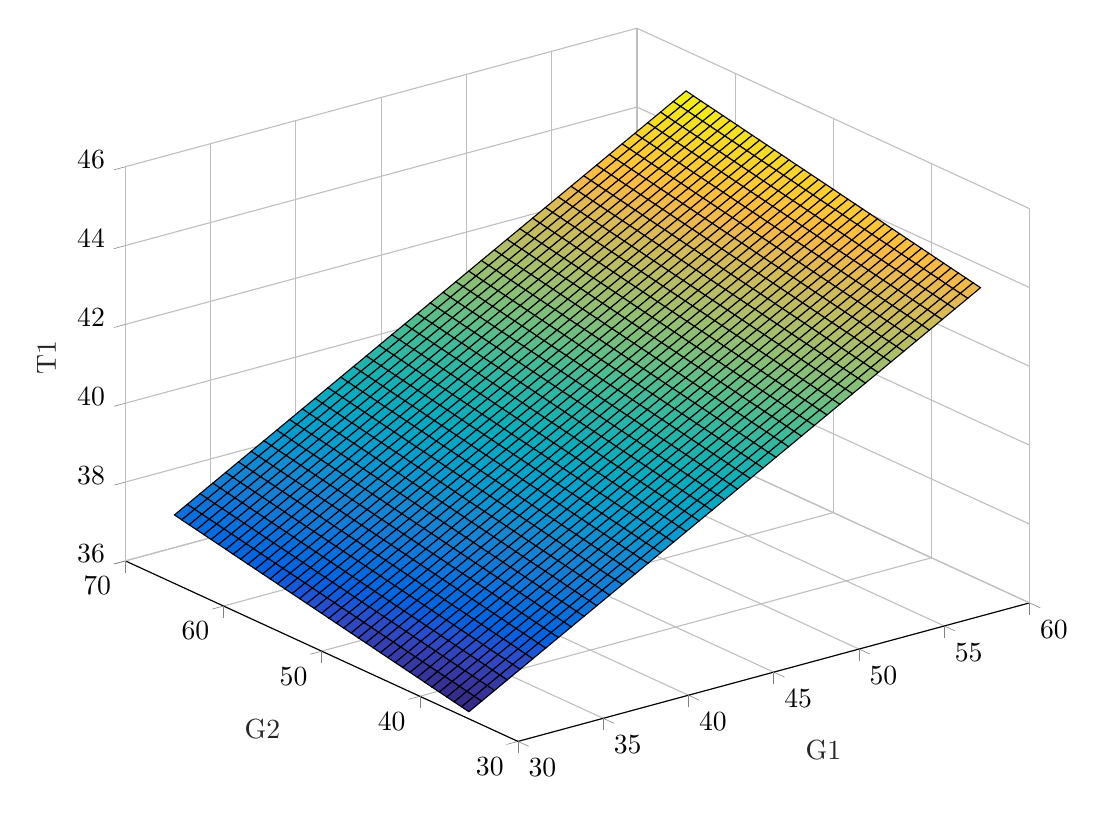
\begin{tikzpicture}

\begin{axis}[%
width=4.521in,
height=3.566in,
at={(0.758in,0.481in)},
scale only axis,
xmin=30,
xmax=60,
tick align=outside,
xlabel style={font=\color{white!15!black}},
xlabel={G1},
ymin=30,
ymax=70,
ylabel style={font=\color{white!15!black}},
ylabel={G2},
zmin=36,
zmax=46,
zlabel style={font=\color{white!15!black}},
zlabel={T1},
view={-37.5}{30},
axis background/.style={fill=white},
axis x line*=bottom,
axis y line*=left,
axis z line*=left,
xmajorgrids,
ymajorgrids,
zmajorgrids
]

\addplot3[%
surf,
shader=flat corner, draw=black, z buffer=sort, colormap={mymap}{[1pt] rgb(0pt)=(0.2081,0.1663,0.5292); rgb(1pt)=(0.211624,0.189781,0.577676); rgb(2pt)=(0.212252,0.213771,0.626971); rgb(3pt)=(0.2081,0.2386,0.677086); rgb(4pt)=(0.195905,0.264457,0.7279); rgb(5pt)=(0.170729,0.291938,0.779248); rgb(6pt)=(0.125271,0.324243,0.830271); rgb(7pt)=(0.0591333,0.359833,0.868333); rgb(8pt)=(0.0116952,0.38751,0.881957); rgb(9pt)=(0.00595714,0.408614,0.882843); rgb(10pt)=(0.0165143,0.4266,0.878633); rgb(11pt)=(0.0328524,0.443043,0.871957); rgb(12pt)=(0.0498143,0.458571,0.864057); rgb(13pt)=(0.0629333,0.47369,0.855438); rgb(14pt)=(0.0722667,0.488667,0.8467); rgb(15pt)=(0.0779429,0.503986,0.838371); rgb(16pt)=(0.0793476,0.520024,0.831181); rgb(17pt)=(0.0749429,0.537543,0.826271); rgb(18pt)=(0.0640571,0.556986,0.823957); rgb(19pt)=(0.0487714,0.577224,0.822829); rgb(20pt)=(0.0343429,0.596581,0.819852); rgb(21pt)=(0.0265,0.6137,0.8135); rgb(22pt)=(0.0238905,0.628662,0.803762); rgb(23pt)=(0.0230905,0.641786,0.791267); rgb(24pt)=(0.0227714,0.653486,0.776757); rgb(25pt)=(0.0266619,0.664195,0.760719); rgb(26pt)=(0.0383714,0.674271,0.743552); rgb(27pt)=(0.0589714,0.683757,0.725386); rgb(28pt)=(0.0843,0.692833,0.706167); rgb(29pt)=(0.113295,0.7015,0.685857); rgb(30pt)=(0.145271,0.709757,0.664629); rgb(31pt)=(0.180133,0.717657,0.642433); rgb(32pt)=(0.217829,0.725043,0.619262); rgb(33pt)=(0.258643,0.731714,0.595429); rgb(34pt)=(0.302171,0.737605,0.571186); rgb(35pt)=(0.348167,0.742433,0.547267); rgb(36pt)=(0.395257,0.7459,0.524443); rgb(37pt)=(0.44201,0.748081,0.503314); rgb(38pt)=(0.487124,0.749062,0.483976); rgb(39pt)=(0.530029,0.749114,0.466114); rgb(40pt)=(0.570857,0.748519,0.44939); rgb(41pt)=(0.609852,0.747314,0.433686); rgb(42pt)=(0.6473,0.7456,0.4188); rgb(43pt)=(0.683419,0.743476,0.404433); rgb(44pt)=(0.71841,0.741133,0.390476); rgb(45pt)=(0.752486,0.7384,0.376814); rgb(46pt)=(0.785843,0.735567,0.363271); rgb(47pt)=(0.818505,0.732733,0.34979); rgb(48pt)=(0.850657,0.7299,0.336029); rgb(49pt)=(0.882433,0.727433,0.3217); rgb(50pt)=(0.913933,0.725786,0.306276); rgb(51pt)=(0.944957,0.726114,0.288643); rgb(52pt)=(0.973895,0.731395,0.266648); rgb(53pt)=(0.993771,0.745457,0.240348); rgb(54pt)=(0.999043,0.765314,0.216414); rgb(55pt)=(0.995533,0.786057,0.196652); rgb(56pt)=(0.988,0.8066,0.179367); rgb(57pt)=(0.978857,0.827143,0.163314); rgb(58pt)=(0.9697,0.848138,0.147452); rgb(59pt)=(0.962586,0.870514,0.1309); rgb(60pt)=(0.958871,0.8949,0.113243); rgb(61pt)=(0.959824,0.921833,0.0948381); rgb(62pt)=(0.9661,0.951443,0.0755333); rgb(63pt)=(0.9763,0.9831,0.0538)}, mesh/rows=41]
table[row sep=crcr, point meta=\thisrow{c}] {%
%
x	y	z	c\\
30	35	36.18	36.18\\
30	35.75	36.218952	36.218952\\
30	36.5	36.257904	36.257904\\
30	37.25	36.296856	36.296856\\
30	38	36.335808	36.335808\\
30	38.75	36.37476	36.37476\\
30	39.5	36.413712	36.413712\\
30	40.25	36.452664	36.452664\\
30	41	36.491616	36.491616\\
30	41.75	36.530568	36.530568\\
30	42.5	36.56952	36.56952\\
30	43.25	36.608472	36.608472\\
30	44	36.647424	36.647424\\
30	44.75	36.686376	36.686376\\
30	45.5	36.725328	36.725328\\
30	46.25	36.76428	36.76428\\
30	47	36.803232	36.803232\\
30	47.75	36.842184	36.842184\\
30	48.5	36.881136	36.881136\\
30	49.25	36.920088	36.920088\\
30	50	36.95904	36.95904\\
30	50.75	36.997992	36.997992\\
30	51.5	37.036944	37.036944\\
30	52.25	37.075896	37.075896\\
30	53	37.114848	37.114848\\
30	53.75	37.1538	37.1538\\
30	54.5	37.192752	37.192752\\
30	55.25	37.231704	37.231704\\
30	56	37.270656	37.270656\\
30	56.75	37.309608	37.309608\\
30	57.5	37.34856	37.34856\\
30	58.25	37.387512	37.387512\\
30	59	37.426464	37.426464\\
30	59.75	37.465416	37.465416\\
30	60.5	37.504368	37.504368\\
30	61.25	37.54332	37.54332\\
30	62	37.582272	37.582272\\
30	62.75	37.621224	37.621224\\
30	63.5	37.660176	37.660176\\
30	64.25	37.699128	37.699128\\
30	65	37.73808	37.73808\\
30.75	35	36.36108	36.36108\\
30.75	35.75	36.400032	36.400032\\
30.75	36.5	36.438984	36.438984\\
30.75	37.25	36.477936	36.477936\\
30.75	38	36.516888	36.516888\\
30.75	38.75	36.55584	36.55584\\
30.75	39.5	36.594792	36.594792\\
30.75	40.25	36.633744	36.633744\\
30.75	41	36.672696	36.672696\\
30.75	41.75	36.711648	36.711648\\
30.75	42.5	36.7506	36.7506\\
30.75	43.25	36.789552	36.789552\\
30.75	44	36.828504	36.828504\\
30.75	44.75	36.867456	36.867456\\
30.75	45.5	36.906408	36.906408\\
30.75	46.25	36.94536	36.94536\\
30.75	47	36.984312	36.984312\\
30.75	47.75	37.023264	37.023264\\
30.75	48.5	37.062216	37.062216\\
30.75	49.25	37.101168	37.101168\\
30.75	50	37.14012	37.14012\\
30.75	50.75	37.179072	37.179072\\
30.75	51.5	37.218024	37.218024\\
30.75	52.25	37.256976	37.256976\\
30.75	53	37.295928	37.295928\\
30.75	53.75	37.33488	37.33488\\
30.75	54.5	37.373832	37.373832\\
30.75	55.25	37.412784	37.412784\\
30.75	56	37.451736	37.451736\\
30.75	56.75	37.490688	37.490688\\
30.75	57.5	37.52964	37.52964\\
30.75	58.25	37.568592	37.568592\\
30.75	59	37.607544	37.607544\\
30.75	59.75	37.646496	37.646496\\
30.75	60.5	37.685448	37.685448\\
30.75	61.25	37.7244	37.7244\\
30.75	62	37.763352	37.763352\\
30.75	62.75	37.802304	37.802304\\
30.75	63.5	37.841256	37.841256\\
30.75	64.25	37.880208	37.880208\\
30.75	65	37.91916	37.91916\\
31.5	35	36.54216	36.54216\\
31.5	35.75	36.581112	36.581112\\
31.5	36.5	36.620064	36.620064\\
31.5	37.25	36.659016	36.659016\\
31.5	38	36.697968	36.697968\\
31.5	38.75	36.73692	36.73692\\
31.5	39.5	36.775872	36.775872\\
31.5	40.25	36.814824	36.814824\\
31.5	41	36.853776	36.853776\\
31.5	41.75	36.892728	36.892728\\
31.5	42.5	36.93168	36.93168\\
31.5	43.25	36.970632	36.970632\\
31.5	44	37.009584	37.009584\\
31.5	44.75	37.048536	37.048536\\
31.5	45.5	37.087488	37.087488\\
31.5	46.25	37.12644	37.12644\\
31.5	47	37.165392	37.165392\\
31.5	47.75	37.204344	37.204344\\
31.5	48.5	37.243296	37.243296\\
31.5	49.25	37.282248	37.282248\\
31.5	50	37.3212	37.3212\\
31.5	50.75	37.360152	37.360152\\
31.5	51.5	37.399104	37.399104\\
31.5	52.25	37.438056	37.438056\\
31.5	53	37.477008	37.477008\\
31.5	53.75	37.51596	37.51596\\
31.5	54.5	37.554912	37.554912\\
31.5	55.25	37.593864	37.593864\\
31.5	56	37.632816	37.632816\\
31.5	56.75	37.671768	37.671768\\
31.5	57.5	37.71072	37.71072\\
31.5	58.25	37.749672	37.749672\\
31.5	59	37.788624	37.788624\\
31.5	59.75	37.827576	37.827576\\
31.5	60.5	37.866528	37.866528\\
31.5	61.25	37.90548	37.90548\\
31.5	62	37.944432	37.944432\\
31.5	62.75	37.983384	37.983384\\
31.5	63.5	38.022336	38.022336\\
31.5	64.25	38.061288	38.061288\\
31.5	65	38.10024	38.10024\\
32.25	35	36.72324	36.72324\\
32.25	35.75	36.762192	36.762192\\
32.25	36.5	36.801144	36.801144\\
32.25	37.25	36.840096	36.840096\\
32.25	38	36.879048	36.879048\\
32.25	38.75	36.918	36.918\\
32.25	39.5	36.956952	36.956952\\
32.25	40.25	36.995904	36.995904\\
32.25	41	37.034856	37.034856\\
32.25	41.75	37.073808	37.073808\\
32.25	42.5	37.11276	37.11276\\
32.25	43.25	37.151712	37.151712\\
32.25	44	37.190664	37.190664\\
32.25	44.75	37.229616	37.229616\\
32.25	45.5	37.268568	37.268568\\
32.25	46.25	37.30752	37.30752\\
32.25	47	37.346472	37.346472\\
32.25	47.75	37.385424	37.385424\\
32.25	48.5	37.424376	37.424376\\
32.25	49.25	37.463328	37.463328\\
32.25	50	37.50228	37.50228\\
32.25	50.75	37.541232	37.541232\\
32.25	51.5	37.580184	37.580184\\
32.25	52.25	37.619136	37.619136\\
32.25	53	37.658088	37.658088\\
32.25	53.75	37.69704	37.69704\\
32.25	54.5	37.735992	37.735992\\
32.25	55.25	37.774944	37.774944\\
32.25	56	37.813896	37.813896\\
32.25	56.75	37.852848	37.852848\\
32.25	57.5	37.8918	37.8918\\
32.25	58.25	37.930752	37.930752\\
32.25	59	37.969704	37.969704\\
32.25	59.75	38.008656	38.008656\\
32.25	60.5	38.047608	38.047608\\
32.25	61.25	38.08656	38.08656\\
32.25	62	38.125512	38.125512\\
32.25	62.75	38.164464	38.164464\\
32.25	63.5	38.203416	38.203416\\
32.25	64.25	38.242368	38.242368\\
32.25	65	38.28132	38.28132\\
33	35	36.90432	36.90432\\
33	35.75	36.943272	36.943272\\
33	36.5	36.982224	36.982224\\
33	37.25	37.021176	37.021176\\
33	38	37.060128	37.060128\\
33	38.75	37.09908	37.09908\\
33	39.5	37.138032	37.138032\\
33	40.25	37.176984	37.176984\\
33	41	37.215936	37.215936\\
33	41.75	37.254888	37.254888\\
33	42.5	37.29384	37.29384\\
33	43.25	37.332792	37.332792\\
33	44	37.371744	37.371744\\
33	44.75	37.410696	37.410696\\
33	45.5	37.449648	37.449648\\
33	46.25	37.4886	37.4886\\
33	47	37.527552	37.527552\\
33	47.75	37.566504	37.566504\\
33	48.5	37.605456	37.605456\\
33	49.25	37.644408	37.644408\\
33	50	37.68336	37.68336\\
33	50.75	37.722312	37.722312\\
33	51.5	37.761264	37.761264\\
33	52.25	37.800216	37.800216\\
33	53	37.839168	37.839168\\
33	53.75	37.87812	37.87812\\
33	54.5	37.917072	37.917072\\
33	55.25	37.956024	37.956024\\
33	56	37.994976	37.994976\\
33	56.75	38.033928	38.033928\\
33	57.5	38.07288	38.07288\\
33	58.25	38.111832	38.111832\\
33	59	38.150784	38.150784\\
33	59.75	38.189736	38.189736\\
33	60.5	38.228688	38.228688\\
33	61.25	38.26764	38.26764\\
33	62	38.306592	38.306592\\
33	62.75	38.345544	38.345544\\
33	63.5	38.384496	38.384496\\
33	64.25	38.423448	38.423448\\
33	65	38.4624	38.4624\\
33.75	35	37.0854	37.0854\\
33.75	35.75	37.124352	37.124352\\
33.75	36.5	37.163304	37.163304\\
33.75	37.25	37.202256	37.202256\\
33.75	38	37.241208	37.241208\\
33.75	38.75	37.28016	37.28016\\
33.75	39.5	37.319112	37.319112\\
33.75	40.25	37.358064	37.358064\\
33.75	41	37.397016	37.397016\\
33.75	41.75	37.435968	37.435968\\
33.75	42.5	37.47492	37.47492\\
33.75	43.25	37.513872	37.513872\\
33.75	44	37.552824	37.552824\\
33.75	44.75	37.591776	37.591776\\
33.75	45.5	37.630728	37.630728\\
33.75	46.25	37.66968	37.66968\\
33.75	47	37.708632	37.708632\\
33.75	47.75	37.747584	37.747584\\
33.75	48.5	37.786536	37.786536\\
33.75	49.25	37.825488	37.825488\\
33.75	50	37.86444	37.86444\\
33.75	50.75	37.903392	37.903392\\
33.75	51.5	37.942344	37.942344\\
33.75	52.25	37.981296	37.981296\\
33.75	53	38.020248	38.020248\\
33.75	53.75	38.0592	38.0592\\
33.75	54.5	38.098152	38.098152\\
33.75	55.25	38.137104	38.137104\\
33.75	56	38.176056	38.176056\\
33.75	56.75	38.215008	38.215008\\
33.75	57.5	38.25396	38.25396\\
33.75	58.25	38.292912	38.292912\\
33.75	59	38.331864	38.331864\\
33.75	59.75	38.370816	38.370816\\
33.75	60.5	38.409768	38.409768\\
33.75	61.25	38.44872	38.44872\\
33.75	62	38.487672	38.487672\\
33.75	62.75	38.526624	38.526624\\
33.75	63.5	38.565576	38.565576\\
33.75	64.25	38.604528	38.604528\\
33.75	65	38.64348	38.64348\\
34.5	35	37.26648	37.26648\\
34.5	35.75	37.305432	37.305432\\
34.5	36.5	37.344384	37.344384\\
34.5	37.25	37.383336	37.383336\\
34.5	38	37.422288	37.422288\\
34.5	38.75	37.46124	37.46124\\
34.5	39.5	37.500192	37.500192\\
34.5	40.25	37.539144	37.539144\\
34.5	41	37.578096	37.578096\\
34.5	41.75	37.617048	37.617048\\
34.5	42.5	37.656	37.656\\
34.5	43.25	37.694952	37.694952\\
34.5	44	37.733904	37.733904\\
34.5	44.75	37.772856	37.772856\\
34.5	45.5	37.811808	37.811808\\
34.5	46.25	37.85076	37.85076\\
34.5	47	37.889712	37.889712\\
34.5	47.75	37.928664	37.928664\\
34.5	48.5	37.967616	37.967616\\
34.5	49.25	38.006568	38.006568\\
34.5	50	38.04552	38.04552\\
34.5	50.75	38.084472	38.084472\\
34.5	51.5	38.123424	38.123424\\
34.5	52.25	38.162376	38.162376\\
34.5	53	38.201328	38.201328\\
34.5	53.75	38.24028	38.24028\\
34.5	54.5	38.279232	38.279232\\
34.5	55.25	38.318184	38.318184\\
34.5	56	38.357136	38.357136\\
34.5	56.75	38.396088	38.396088\\
34.5	57.5	38.43504	38.43504\\
34.5	58.25	38.473992	38.473992\\
34.5	59	38.512944	38.512944\\
34.5	59.75	38.551896	38.551896\\
34.5	60.5	38.590848	38.590848\\
34.5	61.25	38.6298	38.6298\\
34.5	62	38.668752	38.668752\\
34.5	62.75	38.707704	38.707704\\
34.5	63.5	38.746656	38.746656\\
34.5	64.25	38.785608	38.785608\\
34.5	65	38.82456	38.82456\\
35.25	35	37.44756	37.44756\\
35.25	35.75	37.486512	37.486512\\
35.25	36.5	37.525464	37.525464\\
35.25	37.25	37.564416	37.564416\\
35.25	38	37.603368	37.603368\\
35.25	38.75	37.64232	37.64232\\
35.25	39.5	37.681272	37.681272\\
35.25	40.25	37.720224	37.720224\\
35.25	41	37.759176	37.759176\\
35.25	41.75	37.798128	37.798128\\
35.25	42.5	37.83708	37.83708\\
35.25	43.25	37.876032	37.876032\\
35.25	44	37.914984	37.914984\\
35.25	44.75	37.953936	37.953936\\
35.25	45.5	37.992888	37.992888\\
35.25	46.25	38.03184	38.03184\\
35.25	47	38.070792	38.070792\\
35.25	47.75	38.109744	38.109744\\
35.25	48.5	38.148696	38.148696\\
35.25	49.25	38.187648	38.187648\\
35.25	50	38.2266	38.2266\\
35.25	50.75	38.265552	38.265552\\
35.25	51.5	38.304504	38.304504\\
35.25	52.25	38.343456	38.343456\\
35.25	53	38.382408	38.382408\\
35.25	53.75	38.42136	38.42136\\
35.25	54.5	38.460312	38.460312\\
35.25	55.25	38.499264	38.499264\\
35.25	56	38.538216	38.538216\\
35.25	56.75	38.577168	38.577168\\
35.25	57.5	38.61612	38.61612\\
35.25	58.25	38.655072	38.655072\\
35.25	59	38.694024	38.694024\\
35.25	59.75	38.732976	38.732976\\
35.25	60.5	38.771928	38.771928\\
35.25	61.25	38.81088	38.81088\\
35.25	62	38.849832	38.849832\\
35.25	62.75	38.888784	38.888784\\
35.25	63.5	38.927736	38.927736\\
35.25	64.25	38.966688	38.966688\\
35.25	65	39.00564	39.00564\\
36	35	37.62864	37.62864\\
36	35.75	37.667592	37.667592\\
36	36.5	37.706544	37.706544\\
36	37.25	37.745496	37.745496\\
36	38	37.784448	37.784448\\
36	38.75	37.8234	37.8234\\
36	39.5	37.862352	37.862352\\
36	40.25	37.901304	37.901304\\
36	41	37.940256	37.940256\\
36	41.75	37.979208	37.979208\\
36	42.5	38.01816	38.01816\\
36	43.25	38.057112	38.057112\\
36	44	38.096064	38.096064\\
36	44.75	38.135016	38.135016\\
36	45.5	38.173968	38.173968\\
36	46.25	38.21292	38.21292\\
36	47	38.251872	38.251872\\
36	47.75	38.290824	38.290824\\
36	48.5	38.329776	38.329776\\
36	49.25	38.368728	38.368728\\
36	50	38.40768	38.40768\\
36	50.75	38.446632	38.446632\\
36	51.5	38.485584	38.485584\\
36	52.25	38.524536	38.524536\\
36	53	38.563488	38.563488\\
36	53.75	38.60244	38.60244\\
36	54.5	38.641392	38.641392\\
36	55.25	38.680344	38.680344\\
36	56	38.719296	38.719296\\
36	56.75	38.758248	38.758248\\
36	57.5	38.7972	38.7972\\
36	58.25	38.836152	38.836152\\
36	59	38.875104	38.875104\\
36	59.75	38.914056	38.914056\\
36	60.5	38.953008	38.953008\\
36	61.25	38.99196	38.99196\\
36	62	39.030912	39.030912\\
36	62.75	39.069864	39.069864\\
36	63.5	39.108816	39.108816\\
36	64.25	39.147768	39.147768\\
36	65	39.18672	39.18672\\
36.75	35	37.80972	37.80972\\
36.75	35.75	37.848672	37.848672\\
36.75	36.5	37.887624	37.887624\\
36.75	37.25	37.926576	37.926576\\
36.75	38	37.965528	37.965528\\
36.75	38.75	38.00448	38.00448\\
36.75	39.5	38.043432	38.043432\\
36.75	40.25	38.082384	38.082384\\
36.75	41	38.121336	38.121336\\
36.75	41.75	38.160288	38.160288\\
36.75	42.5	38.19924	38.19924\\
36.75	43.25	38.238192	38.238192\\
36.75	44	38.277144	38.277144\\
36.75	44.75	38.316096	38.316096\\
36.75	45.5	38.355048	38.355048\\
36.75	46.25	38.394	38.394\\
36.75	47	38.432952	38.432952\\
36.75	47.75	38.471904	38.471904\\
36.75	48.5	38.510856	38.510856\\
36.75	49.25	38.549808	38.549808\\
36.75	50	38.58876	38.58876\\
36.75	50.75	38.627712	38.627712\\
36.75	51.5	38.666664	38.666664\\
36.75	52.25	38.705616	38.705616\\
36.75	53	38.744568	38.744568\\
36.75	53.75	38.78352	38.78352\\
36.75	54.5	38.822472	38.822472\\
36.75	55.25	38.861424	38.861424\\
36.75	56	38.900376	38.900376\\
36.75	56.75	38.939328	38.939328\\
36.75	57.5	38.97828	38.97828\\
36.75	58.25	39.017232	39.017232\\
36.75	59	39.056184	39.056184\\
36.75	59.75	39.095136	39.095136\\
36.75	60.5	39.134088	39.134088\\
36.75	61.25	39.17304	39.17304\\
36.75	62	39.211992	39.211992\\
36.75	62.75	39.250944	39.250944\\
36.75	63.5	39.289896	39.289896\\
36.75	64.25	39.328848	39.328848\\
36.75	65	39.3678	39.3678\\
37.5	35	37.9908	37.9908\\
37.5	35.75	38.029752	38.029752\\
37.5	36.5	38.068704	38.068704\\
37.5	37.25	38.107656	38.107656\\
37.5	38	38.146608	38.146608\\
37.5	38.75	38.18556	38.18556\\
37.5	39.5	38.224512	38.224512\\
37.5	40.25	38.263464	38.263464\\
37.5	41	38.302416	38.302416\\
37.5	41.75	38.341368	38.341368\\
37.5	42.5	38.38032	38.38032\\
37.5	43.25	38.419272	38.419272\\
37.5	44	38.458224	38.458224\\
37.5	44.75	38.497176	38.497176\\
37.5	45.5	38.536128	38.536128\\
37.5	46.25	38.57508	38.57508\\
37.5	47	38.614032	38.614032\\
37.5	47.75	38.652984	38.652984\\
37.5	48.5	38.691936	38.691936\\
37.5	49.25	38.730888	38.730888\\
37.5	50	38.76984	38.76984\\
37.5	50.75	38.808792	38.808792\\
37.5	51.5	38.847744	38.847744\\
37.5	52.25	38.886696	38.886696\\
37.5	53	38.925648	38.925648\\
37.5	53.75	38.9646	38.9646\\
37.5	54.5	39.003552	39.003552\\
37.5	55.25	39.042504	39.042504\\
37.5	56	39.081456	39.081456\\
37.5	56.75	39.120408	39.120408\\
37.5	57.5	39.15936	39.15936\\
37.5	58.25	39.198312	39.198312\\
37.5	59	39.237264	39.237264\\
37.5	59.75	39.276216	39.276216\\
37.5	60.5	39.315168	39.315168\\
37.5	61.25	39.35412	39.35412\\
37.5	62	39.393072	39.393072\\
37.5	62.75	39.432024	39.432024\\
37.5	63.5	39.470976	39.470976\\
37.5	64.25	39.509928	39.509928\\
37.5	65	39.54888	39.54888\\
38.25	35	38.17188	38.17188\\
38.25	35.75	38.210832	38.210832\\
38.25	36.5	38.249784	38.249784\\
38.25	37.25	38.288736	38.288736\\
38.25	38	38.327688	38.327688\\
38.25	38.75	38.36664	38.36664\\
38.25	39.5	38.405592	38.405592\\
38.25	40.25	38.444544	38.444544\\
38.25	41	38.483496	38.483496\\
38.25	41.75	38.522448	38.522448\\
38.25	42.5	38.5614	38.5614\\
38.25	43.25	38.600352	38.600352\\
38.25	44	38.639304	38.639304\\
38.25	44.75	38.678256	38.678256\\
38.25	45.5	38.717208	38.717208\\
38.25	46.25	38.75616	38.75616\\
38.25	47	38.795112	38.795112\\
38.25	47.75	38.834064	38.834064\\
38.25	48.5	38.873016	38.873016\\
38.25	49.25	38.911968	38.911968\\
38.25	50	38.95092	38.95092\\
38.25	50.75	38.989872	38.989872\\
38.25	51.5	39.028824	39.028824\\
38.25	52.25	39.067776	39.067776\\
38.25	53	39.106728	39.106728\\
38.25	53.75	39.14568	39.14568\\
38.25	54.5	39.184632	39.184632\\
38.25	55.25	39.223584	39.223584\\
38.25	56	39.262536	39.262536\\
38.25	56.75	39.301488	39.301488\\
38.25	57.5	39.34044	39.34044\\
38.25	58.25	39.379392	39.379392\\
38.25	59	39.418344	39.418344\\
38.25	59.75	39.457296	39.457296\\
38.25	60.5	39.496248	39.496248\\
38.25	61.25	39.5352	39.5352\\
38.25	62	39.574152	39.574152\\
38.25	62.75	39.613104	39.613104\\
38.25	63.5	39.652056	39.652056\\
38.25	64.25	39.691008	39.691008\\
38.25	65	39.72996	39.72996\\
39	35	38.35296	38.35296\\
39	35.75	38.391912	38.391912\\
39	36.5	38.430864	38.430864\\
39	37.25	38.469816	38.469816\\
39	38	38.508768	38.508768\\
39	38.75	38.54772	38.54772\\
39	39.5	38.586672	38.586672\\
39	40.25	38.625624	38.625624\\
39	41	38.664576	38.664576\\
39	41.75	38.703528	38.703528\\
39	42.5	38.74248	38.74248\\
39	43.25	38.781432	38.781432\\
39	44	38.820384	38.820384\\
39	44.75	38.859336	38.859336\\
39	45.5	38.898288	38.898288\\
39	46.25	38.93724	38.93724\\
39	47	38.976192	38.976192\\
39	47.75	39.015144	39.015144\\
39	48.5	39.054096	39.054096\\
39	49.25	39.093048	39.093048\\
39	50	39.132	39.132\\
39	50.75	39.170952	39.170952\\
39	51.5	39.209904	39.209904\\
39	52.25	39.248856	39.248856\\
39	53	39.287808	39.287808\\
39	53.75	39.32676	39.32676\\
39	54.5	39.365712	39.365712\\
39	55.25	39.404664	39.404664\\
39	56	39.443616	39.443616\\
39	56.75	39.482568	39.482568\\
39	57.5	39.52152	39.52152\\
39	58.25	39.560472	39.560472\\
39	59	39.599424	39.599424\\
39	59.75	39.638376	39.638376\\
39	60.5	39.677328	39.677328\\
39	61.25	39.71628	39.71628\\
39	62	39.755232	39.755232\\
39	62.75	39.794184	39.794184\\
39	63.5	39.833136	39.833136\\
39	64.25	39.872088	39.872088\\
39	65	39.91104	39.91104\\
39.75	35	38.53404	38.53404\\
39.75	35.75	38.572992	38.572992\\
39.75	36.5	38.611944	38.611944\\
39.75	37.25	38.650896	38.650896\\
39.75	38	38.689848	38.689848\\
39.75	38.75	38.7288	38.7288\\
39.75	39.5	38.767752	38.767752\\
39.75	40.25	38.806704	38.806704\\
39.75	41	38.845656	38.845656\\
39.75	41.75	38.884608	38.884608\\
39.75	42.5	38.92356	38.92356\\
39.75	43.25	38.962512	38.962512\\
39.75	44	39.001464	39.001464\\
39.75	44.75	39.040416	39.040416\\
39.75	45.5	39.079368	39.079368\\
39.75	46.25	39.11832	39.11832\\
39.75	47	39.157272	39.157272\\
39.75	47.75	39.196224	39.196224\\
39.75	48.5	39.235176	39.235176\\
39.75	49.25	39.274128	39.274128\\
39.75	50	39.31308	39.31308\\
39.75	50.75	39.352032	39.352032\\
39.75	51.5	39.390984	39.390984\\
39.75	52.25	39.429936	39.429936\\
39.75	53	39.468888	39.468888\\
39.75	53.75	39.50784	39.50784\\
39.75	54.5	39.546792	39.546792\\
39.75	55.25	39.585744	39.585744\\
39.75	56	39.624696	39.624696\\
39.75	56.75	39.663648	39.663648\\
39.75	57.5	39.7026	39.7026\\
39.75	58.25	39.741552	39.741552\\
39.75	59	39.780504	39.780504\\
39.75	59.75	39.819456	39.819456\\
39.75	60.5	39.858408	39.858408\\
39.75	61.25	39.89736	39.89736\\
39.75	62	39.936312	39.936312\\
39.75	62.75	39.975264	39.975264\\
39.75	63.5	40.014216	40.014216\\
39.75	64.25	40.053168	40.053168\\
39.75	65	40.09212	40.09212\\
40.5	35	38.71512	38.71512\\
40.5	35.75	38.754072	38.754072\\
40.5	36.5	38.793024	38.793024\\
40.5	37.25	38.831976	38.831976\\
40.5	38	38.870928	38.870928\\
40.5	38.75	38.90988	38.90988\\
40.5	39.5	38.948832	38.948832\\
40.5	40.25	38.987784	38.987784\\
40.5	41	39.026736	39.026736\\
40.5	41.75	39.065688	39.065688\\
40.5	42.5	39.10464	39.10464\\
40.5	43.25	39.143592	39.143592\\
40.5	44	39.182544	39.182544\\
40.5	44.75	39.221496	39.221496\\
40.5	45.5	39.260448	39.260448\\
40.5	46.25	39.2994	39.2994\\
40.5	47	39.338352	39.338352\\
40.5	47.75	39.377304	39.377304\\
40.5	48.5	39.416256	39.416256\\
40.5	49.25	39.455208	39.455208\\
40.5	50	39.49416	39.49416\\
40.5	50.75	39.533112	39.533112\\
40.5	51.5	39.572064	39.572064\\
40.5	52.25	39.611016	39.611016\\
40.5	53	39.649968	39.649968\\
40.5	53.75	39.68892	39.68892\\
40.5	54.5	39.727872	39.727872\\
40.5	55.25	39.766824	39.766824\\
40.5	56	39.805776	39.805776\\
40.5	56.75	39.844728	39.844728\\
40.5	57.5	39.88368	39.88368\\
40.5	58.25	39.922632	39.922632\\
40.5	59	39.961584	39.961584\\
40.5	59.75	40.000536	40.000536\\
40.5	60.5	40.039488	40.039488\\
40.5	61.25	40.07844	40.07844\\
40.5	62	40.117392	40.117392\\
40.5	62.75	40.156344	40.156344\\
40.5	63.5	40.195296	40.195296\\
40.5	64.25	40.234248	40.234248\\
40.5	65	40.2732	40.2732\\
41.25	35	38.8962	38.8962\\
41.25	35.75	38.935152	38.935152\\
41.25	36.5	38.974104	38.974104\\
41.25	37.25	39.013056	39.013056\\
41.25	38	39.052008	39.052008\\
41.25	38.75	39.09096	39.09096\\
41.25	39.5	39.129912	39.129912\\
41.25	40.25	39.168864	39.168864\\
41.25	41	39.207816	39.207816\\
41.25	41.75	39.246768	39.246768\\
41.25	42.5	39.28572	39.28572\\
41.25	43.25	39.324672	39.324672\\
41.25	44	39.363624	39.363624\\
41.25	44.75	39.402576	39.402576\\
41.25	45.5	39.441528	39.441528\\
41.25	46.25	39.48048	39.48048\\
41.25	47	39.519432	39.519432\\
41.25	47.75	39.558384	39.558384\\
41.25	48.5	39.597336	39.597336\\
41.25	49.25	39.636288	39.636288\\
41.25	50	39.67524	39.67524\\
41.25	50.75	39.714192	39.714192\\
41.25	51.5	39.753144	39.753144\\
41.25	52.25	39.792096	39.792096\\
41.25	53	39.831048	39.831048\\
41.25	53.75	39.87	39.87\\
41.25	54.5	39.908952	39.908952\\
41.25	55.25	39.947904	39.947904\\
41.25	56	39.986856	39.986856\\
41.25	56.75	40.025808	40.025808\\
41.25	57.5	40.06476	40.06476\\
41.25	58.25	40.103712	40.103712\\
41.25	59	40.142664	40.142664\\
41.25	59.75	40.181616	40.181616\\
41.25	60.5	40.220568	40.220568\\
41.25	61.25	40.25952	40.25952\\
41.25	62	40.298472	40.298472\\
41.25	62.75	40.337424	40.337424\\
41.25	63.5	40.376376	40.376376\\
41.25	64.25	40.415328	40.415328\\
41.25	65	40.45428	40.45428\\
42	35	39.07728	39.07728\\
42	35.75	39.116232	39.116232\\
42	36.5	39.155184	39.155184\\
42	37.25	39.194136	39.194136\\
42	38	39.233088	39.233088\\
42	38.75	39.27204	39.27204\\
42	39.5	39.310992	39.310992\\
42	40.25	39.349944	39.349944\\
42	41	39.388896	39.388896\\
42	41.75	39.427848	39.427848\\
42	42.5	39.4668	39.4668\\
42	43.25	39.505752	39.505752\\
42	44	39.544704	39.544704\\
42	44.75	39.583656	39.583656\\
42	45.5	39.622608	39.622608\\
42	46.25	39.66156	39.66156\\
42	47	39.700512	39.700512\\
42	47.75	39.739464	39.739464\\
42	48.5	39.778416	39.778416\\
42	49.25	39.817368	39.817368\\
42	50	39.85632	39.85632\\
42	50.75	39.895272	39.895272\\
42	51.5	39.934224	39.934224\\
42	52.25	39.973176	39.973176\\
42	53	40.012128	40.012128\\
42	53.75	40.05108	40.05108\\
42	54.5	40.090032	40.090032\\
42	55.25	40.128984	40.128984\\
42	56	40.167936	40.167936\\
42	56.75	40.206888	40.206888\\
42	57.5	40.24584	40.24584\\
42	58.25	40.284792	40.284792\\
42	59	40.323744	40.323744\\
42	59.75	40.362696	40.362696\\
42	60.5	40.401648	40.401648\\
42	61.25	40.4406	40.4406\\
42	62	40.479552	40.479552\\
42	62.75	40.518504	40.518504\\
42	63.5	40.557456	40.557456\\
42	64.25	40.596408	40.596408\\
42	65	40.63536	40.63536\\
42.75	35	39.25836	39.25836\\
42.75	35.75	39.297312	39.297312\\
42.75	36.5	39.336264	39.336264\\
42.75	37.25	39.375216	39.375216\\
42.75	38	39.414168	39.414168\\
42.75	38.75	39.45312	39.45312\\
42.75	39.5	39.492072	39.492072\\
42.75	40.25	39.531024	39.531024\\
42.75	41	39.569976	39.569976\\
42.75	41.75	39.608928	39.608928\\
42.75	42.5	39.64788	39.64788\\
42.75	43.25	39.686832	39.686832\\
42.75	44	39.725784	39.725784\\
42.75	44.75	39.764736	39.764736\\
42.75	45.5	39.803688	39.803688\\
42.75	46.25	39.84264	39.84264\\
42.75	47	39.881592	39.881592\\
42.75	47.75	39.920544	39.920544\\
42.75	48.5	39.959496	39.959496\\
42.75	49.25	39.998448	39.998448\\
42.75	50	40.0374	40.0374\\
42.75	50.75	40.076352	40.076352\\
42.75	51.5	40.115304	40.115304\\
42.75	52.25	40.154256	40.154256\\
42.75	53	40.193208	40.193208\\
42.75	53.75	40.23216	40.23216\\
42.75	54.5	40.271112	40.271112\\
42.75	55.25	40.310064	40.310064\\
42.75	56	40.349016	40.349016\\
42.75	56.75	40.387968	40.387968\\
42.75	57.5	40.42692	40.42692\\
42.75	58.25	40.465872	40.465872\\
42.75	59	40.504824	40.504824\\
42.75	59.75	40.543776	40.543776\\
42.75	60.5	40.582728	40.582728\\
42.75	61.25	40.62168	40.62168\\
42.75	62	40.660632	40.660632\\
42.75	62.75	40.699584	40.699584\\
42.75	63.5	40.738536	40.738536\\
42.75	64.25	40.777488	40.777488\\
42.75	65	40.81644	40.81644\\
43.5	35	39.43944	39.43944\\
43.5	35.75	39.478392	39.478392\\
43.5	36.5	39.517344	39.517344\\
43.5	37.25	39.556296	39.556296\\
43.5	38	39.595248	39.595248\\
43.5	38.75	39.6342	39.6342\\
43.5	39.5	39.673152	39.673152\\
43.5	40.25	39.712104	39.712104\\
43.5	41	39.751056	39.751056\\
43.5	41.75	39.790008	39.790008\\
43.5	42.5	39.82896	39.82896\\
43.5	43.25	39.867912	39.867912\\
43.5	44	39.906864	39.906864\\
43.5	44.75	39.945816	39.945816\\
43.5	45.5	39.984768	39.984768\\
43.5	46.25	40.02372	40.02372\\
43.5	47	40.062672	40.062672\\
43.5	47.75	40.101624	40.101624\\
43.5	48.5	40.140576	40.140576\\
43.5	49.25	40.179528	40.179528\\
43.5	50	40.21848	40.21848\\
43.5	50.75	40.257432	40.257432\\
43.5	51.5	40.296384	40.296384\\
43.5	52.25	40.335336	40.335336\\
43.5	53	40.374288	40.374288\\
43.5	53.75	40.41324	40.41324\\
43.5	54.5	40.452192	40.452192\\
43.5	55.25	40.491144	40.491144\\
43.5	56	40.530096	40.530096\\
43.5	56.75	40.569048	40.569048\\
43.5	57.5	40.608	40.608\\
43.5	58.25	40.646952	40.646952\\
43.5	59	40.685904	40.685904\\
43.5	59.75	40.724856	40.724856\\
43.5	60.5	40.763808	40.763808\\
43.5	61.25	40.80276	40.80276\\
43.5	62	40.841712	40.841712\\
43.5	62.75	40.880664	40.880664\\
43.5	63.5	40.919616	40.919616\\
43.5	64.25	40.958568	40.958568\\
43.5	65	40.99752	40.99752\\
44.25	35	39.62052	39.62052\\
44.25	35.75	39.659472	39.659472\\
44.25	36.5	39.698424	39.698424\\
44.25	37.25	39.737376	39.737376\\
44.25	38	39.776328	39.776328\\
44.25	38.75	39.81528	39.81528\\
44.25	39.5	39.854232	39.854232\\
44.25	40.25	39.893184	39.893184\\
44.25	41	39.932136	39.932136\\
44.25	41.75	39.971088	39.971088\\
44.25	42.5	40.01004	40.01004\\
44.25	43.25	40.048992	40.048992\\
44.25	44	40.087944	40.087944\\
44.25	44.75	40.126896	40.126896\\
44.25	45.5	40.165848	40.165848\\
44.25	46.25	40.2048	40.2048\\
44.25	47	40.243752	40.243752\\
44.25	47.75	40.282704	40.282704\\
44.25	48.5	40.321656	40.321656\\
44.25	49.25	40.360608	40.360608\\
44.25	50	40.39956	40.39956\\
44.25	50.75	40.438512	40.438512\\
44.25	51.5	40.477464	40.477464\\
44.25	52.25	40.516416	40.516416\\
44.25	53	40.555368	40.555368\\
44.25	53.75	40.59432	40.59432\\
44.25	54.5	40.633272	40.633272\\
44.25	55.25	40.672224	40.672224\\
44.25	56	40.711176	40.711176\\
44.25	56.75	40.750128	40.750128\\
44.25	57.5	40.78908	40.78908\\
44.25	58.25	40.828032	40.828032\\
44.25	59	40.866984	40.866984\\
44.25	59.75	40.905936	40.905936\\
44.25	60.5	40.944888	40.944888\\
44.25	61.25	40.98384	40.98384\\
44.25	62	41.022792	41.022792\\
44.25	62.75	41.061744	41.061744\\
44.25	63.5	41.100696	41.100696\\
44.25	64.25	41.139648	41.139648\\
44.25	65	41.1786	41.1786\\
45	35	39.8016	39.8016\\
45	35.75	39.840552	39.840552\\
45	36.5	39.879504	39.879504\\
45	37.25	39.918456	39.918456\\
45	38	39.957408	39.957408\\
45	38.75	39.99636	39.99636\\
45	39.5	40.035312	40.035312\\
45	40.25	40.074264	40.074264\\
45	41	40.113216	40.113216\\
45	41.75	40.152168	40.152168\\
45	42.5	40.19112	40.19112\\
45	43.25	40.230072	40.230072\\
45	44	40.269024	40.269024\\
45	44.75	40.307976	40.307976\\
45	45.5	40.346928	40.346928\\
45	46.25	40.38588	40.38588\\
45	47	40.424832	40.424832\\
45	47.75	40.463784	40.463784\\
45	48.5	40.502736	40.502736\\
45	49.25	40.541688	40.541688\\
45	50	40.58064	40.58064\\
45	50.75	40.619592	40.619592\\
45	51.5	40.658544	40.658544\\
45	52.25	40.697496	40.697496\\
45	53	40.736448	40.736448\\
45	53.75	40.7754	40.7754\\
45	54.5	40.814352	40.814352\\
45	55.25	40.853304	40.853304\\
45	56	40.892256	40.892256\\
45	56.75	40.931208	40.931208\\
45	57.5	40.97016	40.97016\\
45	58.25	41.009112	41.009112\\
45	59	41.048064	41.048064\\
45	59.75	41.087016	41.087016\\
45	60.5	41.125968	41.125968\\
45	61.25	41.16492	41.16492\\
45	62	41.203872	41.203872\\
45	62.75	41.242824	41.242824\\
45	63.5	41.281776	41.281776\\
45	64.25	41.320728	41.320728\\
45	65	41.35968	41.35968\\
45.75	35	39.98268	39.98268\\
45.75	35.75	40.021632	40.021632\\
45.75	36.5	40.060584	40.060584\\
45.75	37.25	40.099536	40.099536\\
45.75	38	40.138488	40.138488\\
45.75	38.75	40.17744	40.17744\\
45.75	39.5	40.216392	40.216392\\
45.75	40.25	40.255344	40.255344\\
45.75	41	40.294296	40.294296\\
45.75	41.75	40.333248	40.333248\\
45.75	42.5	40.3722	40.3722\\
45.75	43.25	40.411152	40.411152\\
45.75	44	40.450104	40.450104\\
45.75	44.75	40.489056	40.489056\\
45.75	45.5	40.528008	40.528008\\
45.75	46.25	40.56696	40.56696\\
45.75	47	40.605912	40.605912\\
45.75	47.75	40.644864	40.644864\\
45.75	48.5	40.683816	40.683816\\
45.75	49.25	40.722768	40.722768\\
45.75	50	40.76172	40.76172\\
45.75	50.75	40.800672	40.800672\\
45.75	51.5	40.839624	40.839624\\
45.75	52.25	40.878576	40.878576\\
45.75	53	40.917528	40.917528\\
45.75	53.75	40.95648	40.95648\\
45.75	54.5	40.995432	40.995432\\
45.75	55.25	41.034384	41.034384\\
45.75	56	41.073336	41.073336\\
45.75	56.75	41.112288	41.112288\\
45.75	57.5	41.15124	41.15124\\
45.75	58.25	41.190192	41.190192\\
45.75	59	41.229144	41.229144\\
45.75	59.75	41.268096	41.268096\\
45.75	60.5	41.307048	41.307048\\
45.75	61.25	41.346	41.346\\
45.75	62	41.384952	41.384952\\
45.75	62.75	41.423904	41.423904\\
45.75	63.5	41.462856	41.462856\\
45.75	64.25	41.501808	41.501808\\
45.75	65	41.54076	41.54076\\
46.5	35	40.16376	40.16376\\
46.5	35.75	40.202712	40.202712\\
46.5	36.5	40.241664	40.241664\\
46.5	37.25	40.280616	40.280616\\
46.5	38	40.319568	40.319568\\
46.5	38.75	40.35852	40.35852\\
46.5	39.5	40.397472	40.397472\\
46.5	40.25	40.436424	40.436424\\
46.5	41	40.475376	40.475376\\
46.5	41.75	40.514328	40.514328\\
46.5	42.5	40.55328	40.55328\\
46.5	43.25	40.592232	40.592232\\
46.5	44	40.631184	40.631184\\
46.5	44.75	40.670136	40.670136\\
46.5	45.5	40.709088	40.709088\\
46.5	46.25	40.74804	40.74804\\
46.5	47	40.786992	40.786992\\
46.5	47.75	40.825944	40.825944\\
46.5	48.5	40.864896	40.864896\\
46.5	49.25	40.903848	40.903848\\
46.5	50	40.9428	40.9428\\
46.5	50.75	40.981752	40.981752\\
46.5	51.5	41.020704	41.020704\\
46.5	52.25	41.059656	41.059656\\
46.5	53	41.098608	41.098608\\
46.5	53.75	41.13756	41.13756\\
46.5	54.5	41.176512	41.176512\\
46.5	55.25	41.215464	41.215464\\
46.5	56	41.254416	41.254416\\
46.5	56.75	41.293368	41.293368\\
46.5	57.5	41.33232	41.33232\\
46.5	58.25	41.371272	41.371272\\
46.5	59	41.410224	41.410224\\
46.5	59.75	41.449176	41.449176\\
46.5	60.5	41.488128	41.488128\\
46.5	61.25	41.52708	41.52708\\
46.5	62	41.566032	41.566032\\
46.5	62.75	41.604984	41.604984\\
46.5	63.5	41.643936	41.643936\\
46.5	64.25	41.682888	41.682888\\
46.5	65	41.72184	41.72184\\
47.25	35	40.34484	40.34484\\
47.25	35.75	40.383792	40.383792\\
47.25	36.5	40.422744	40.422744\\
47.25	37.25	40.461696	40.461696\\
47.25	38	40.500648	40.500648\\
47.25	38.75	40.5396	40.5396\\
47.25	39.5	40.578552	40.578552\\
47.25	40.25	40.617504	40.617504\\
47.25	41	40.656456	40.656456\\
47.25	41.75	40.695408	40.695408\\
47.25	42.5	40.73436	40.73436\\
47.25	43.25	40.773312	40.773312\\
47.25	44	40.812264	40.812264\\
47.25	44.75	40.851216	40.851216\\
47.25	45.5	40.890168	40.890168\\
47.25	46.25	40.92912	40.92912\\
47.25	47	40.968072	40.968072\\
47.25	47.75	41.007024	41.007024\\
47.25	48.5	41.045976	41.045976\\
47.25	49.25	41.084928	41.084928\\
47.25	50	41.12388	41.12388\\
47.25	50.75	41.162832	41.162832\\
47.25	51.5	41.201784	41.201784\\
47.25	52.25	41.240736	41.240736\\
47.25	53	41.279688	41.279688\\
47.25	53.75	41.31864	41.31864\\
47.25	54.5	41.357592	41.357592\\
47.25	55.25	41.396544	41.396544\\
47.25	56	41.435496	41.435496\\
47.25	56.75	41.474448	41.474448\\
47.25	57.5	41.5134	41.5134\\
47.25	58.25	41.552352	41.552352\\
47.25	59	41.591304	41.591304\\
47.25	59.75	41.630256	41.630256\\
47.25	60.5	41.669208	41.669208\\
47.25	61.25	41.70816	41.70816\\
47.25	62	41.747112	41.747112\\
47.25	62.75	41.786064	41.786064\\
47.25	63.5	41.825016	41.825016\\
47.25	64.25	41.863968	41.863968\\
47.25	65	41.90292	41.90292\\
48	35	40.52592	40.52592\\
48	35.75	40.564872	40.564872\\
48	36.5	40.603824	40.603824\\
48	37.25	40.642776	40.642776\\
48	38	40.681728	40.681728\\
48	38.75	40.72068	40.72068\\
48	39.5	40.759632	40.759632\\
48	40.25	40.798584	40.798584\\
48	41	40.837536	40.837536\\
48	41.75	40.876488	40.876488\\
48	42.5	40.91544	40.91544\\
48	43.25	40.954392	40.954392\\
48	44	40.993344	40.993344\\
48	44.75	41.032296	41.032296\\
48	45.5	41.071248	41.071248\\
48	46.25	41.1102	41.1102\\
48	47	41.149152	41.149152\\
48	47.75	41.188104	41.188104\\
48	48.5	41.227056	41.227056\\
48	49.25	41.266008	41.266008\\
48	50	41.30496	41.30496\\
48	50.75	41.343912	41.343912\\
48	51.5	41.382864	41.382864\\
48	52.25	41.421816	41.421816\\
48	53	41.460768	41.460768\\
48	53.75	41.49972	41.49972\\
48	54.5	41.538672	41.538672\\
48	55.25	41.577624	41.577624\\
48	56	41.616576	41.616576\\
48	56.75	41.655528	41.655528\\
48	57.5	41.69448	41.69448\\
48	58.25	41.733432	41.733432\\
48	59	41.772384	41.772384\\
48	59.75	41.811336	41.811336\\
48	60.5	41.850288	41.850288\\
48	61.25	41.88924	41.88924\\
48	62	41.928192	41.928192\\
48	62.75	41.967144	41.967144\\
48	63.5	42.006096	42.006096\\
48	64.25	42.045048	42.045048\\
48	65	42.084	42.084\\
48.75	35	40.707	40.707\\
48.75	35.75	40.745952	40.745952\\
48.75	36.5	40.784904	40.784904\\
48.75	37.25	40.823856	40.823856\\
48.75	38	40.862808	40.862808\\
48.75	38.75	40.90176	40.90176\\
48.75	39.5	40.940712	40.940712\\
48.75	40.25	40.979664	40.979664\\
48.75	41	41.018616	41.018616\\
48.75	41.75	41.057568	41.057568\\
48.75	42.5	41.09652	41.09652\\
48.75	43.25	41.135472	41.135472\\
48.75	44	41.174424	41.174424\\
48.75	44.75	41.213376	41.213376\\
48.75	45.5	41.252328	41.252328\\
48.75	46.25	41.29128	41.29128\\
48.75	47	41.330232	41.330232\\
48.75	47.75	41.369184	41.369184\\
48.75	48.5	41.408136	41.408136\\
48.75	49.25	41.447088	41.447088\\
48.75	50	41.48604	41.48604\\
48.75	50.75	41.524992	41.524992\\
48.75	51.5	41.563944	41.563944\\
48.75	52.25	41.602896	41.602896\\
48.75	53	41.641848	41.641848\\
48.75	53.75	41.6808	41.6808\\
48.75	54.5	41.719752	41.719752\\
48.75	55.25	41.758704	41.758704\\
48.75	56	41.797656	41.797656\\
48.75	56.75	41.836608	41.836608\\
48.75	57.5	41.87556	41.87556\\
48.75	58.25	41.914512	41.914512\\
48.75	59	41.953464	41.953464\\
48.75	59.75	41.992416	41.992416\\
48.75	60.5	42.031368	42.031368\\
48.75	61.25	42.07032	42.07032\\
48.75	62	42.109272	42.109272\\
48.75	62.75	42.148224	42.148224\\
48.75	63.5	42.187176	42.187176\\
48.75	64.25	42.226128	42.226128\\
48.75	65	42.26508	42.26508\\
49.5	35	40.88808	40.88808\\
49.5	35.75	40.927032	40.927032\\
49.5	36.5	40.965984	40.965984\\
49.5	37.25	41.004936	41.004936\\
49.5	38	41.043888	41.043888\\
49.5	38.75	41.08284	41.08284\\
49.5	39.5	41.121792	41.121792\\
49.5	40.25	41.160744	41.160744\\
49.5	41	41.199696	41.199696\\
49.5	41.75	41.238648	41.238648\\
49.5	42.5	41.2776	41.2776\\
49.5	43.25	41.316552	41.316552\\
49.5	44	41.355504	41.355504\\
49.5	44.75	41.394456	41.394456\\
49.5	45.5	41.433408	41.433408\\
49.5	46.25	41.47236	41.47236\\
49.5	47	41.511312	41.511312\\
49.5	47.75	41.550264	41.550264\\
49.5	48.5	41.589216	41.589216\\
49.5	49.25	41.628168	41.628168\\
49.5	50	41.66712	41.66712\\
49.5	50.75	41.706072	41.706072\\
49.5	51.5	41.745024	41.745024\\
49.5	52.25	41.783976	41.783976\\
49.5	53	41.822928	41.822928\\
49.5	53.75	41.86188	41.86188\\
49.5	54.5	41.900832	41.900832\\
49.5	55.25	41.939784	41.939784\\
49.5	56	41.978736	41.978736\\
49.5	56.75	42.017688	42.017688\\
49.5	57.5	42.05664	42.05664\\
49.5	58.25	42.095592	42.095592\\
49.5	59	42.134544	42.134544\\
49.5	59.75	42.173496	42.173496\\
49.5	60.5	42.212448	42.212448\\
49.5	61.25	42.2514	42.2514\\
49.5	62	42.290352	42.290352\\
49.5	62.75	42.329304	42.329304\\
49.5	63.5	42.368256	42.368256\\
49.5	64.25	42.407208	42.407208\\
49.5	65	42.44616	42.44616\\
50.25	35	41.06916	41.06916\\
50.25	35.75	41.108112	41.108112\\
50.25	36.5	41.147064	41.147064\\
50.25	37.25	41.186016	41.186016\\
50.25	38	41.224968	41.224968\\
50.25	38.75	41.26392	41.26392\\
50.25	39.5	41.302872	41.302872\\
50.25	40.25	41.341824	41.341824\\
50.25	41	41.380776	41.380776\\
50.25	41.75	41.419728	41.419728\\
50.25	42.5	41.45868	41.45868\\
50.25	43.25	41.497632	41.497632\\
50.25	44	41.536584	41.536584\\
50.25	44.75	41.575536	41.575536\\
50.25	45.5	41.614488	41.614488\\
50.25	46.25	41.65344	41.65344\\
50.25	47	41.692392	41.692392\\
50.25	47.75	41.731344	41.731344\\
50.25	48.5	41.770296	41.770296\\
50.25	49.25	41.809248	41.809248\\
50.25	50	41.8482	41.8482\\
50.25	50.75	41.887152	41.887152\\
50.25	51.5	41.926104	41.926104\\
50.25	52.25	41.965056	41.965056\\
50.25	53	42.004008	42.004008\\
50.25	53.75	42.04296	42.04296\\
50.25	54.5	42.081912	42.081912\\
50.25	55.25	42.120864	42.120864\\
50.25	56	42.159816	42.159816\\
50.25	56.75	42.198768	42.198768\\
50.25	57.5	42.23772	42.23772\\
50.25	58.25	42.276672	42.276672\\
50.25	59	42.315624	42.315624\\
50.25	59.75	42.354576	42.354576\\
50.25	60.5	42.393528	42.393528\\
50.25	61.25	42.43248	42.43248\\
50.25	62	42.471432	42.471432\\
50.25	62.75	42.510384	42.510384\\
50.25	63.5	42.549336	42.549336\\
50.25	64.25	42.588288	42.588288\\
50.25	65	42.62724	42.62724\\
51	35	41.25024	41.25024\\
51	35.75	41.289192	41.289192\\
51	36.5	41.328144	41.328144\\
51	37.25	41.367096	41.367096\\
51	38	41.406048	41.406048\\
51	38.75	41.445	41.445\\
51	39.5	41.483952	41.483952\\
51	40.25	41.522904	41.522904\\
51	41	41.561856	41.561856\\
51	41.75	41.600808	41.600808\\
51	42.5	41.63976	41.63976\\
51	43.25	41.678712	41.678712\\
51	44	41.717664	41.717664\\
51	44.75	41.756616	41.756616\\
51	45.5	41.795568	41.795568\\
51	46.25	41.83452	41.83452\\
51	47	41.873472	41.873472\\
51	47.75	41.912424	41.912424\\
51	48.5	41.951376	41.951376\\
51	49.25	41.990328	41.990328\\
51	50	42.02928	42.02928\\
51	50.75	42.068232	42.068232\\
51	51.5	42.107184	42.107184\\
51	52.25	42.146136	42.146136\\
51	53	42.185088	42.185088\\
51	53.75	42.22404	42.22404\\
51	54.5	42.262992	42.262992\\
51	55.25	42.301944	42.301944\\
51	56	42.340896	42.340896\\
51	56.75	42.379848	42.379848\\
51	57.5	42.4188	42.4188\\
51	58.25	42.457752	42.457752\\
51	59	42.496704	42.496704\\
51	59.75	42.535656	42.535656\\
51	60.5	42.574608	42.574608\\
51	61.25	42.61356	42.61356\\
51	62	42.652512	42.652512\\
51	62.75	42.691464	42.691464\\
51	63.5	42.730416	42.730416\\
51	64.25	42.769368	42.769368\\
51	65	42.80832	42.80832\\
51.75	35	41.43132	41.43132\\
51.75	35.75	41.470272	41.470272\\
51.75	36.5	41.509224	41.509224\\
51.75	37.25	41.548176	41.548176\\
51.75	38	41.587128	41.587128\\
51.75	38.75	41.62608	41.62608\\
51.75	39.5	41.665032	41.665032\\
51.75	40.25	41.703984	41.703984\\
51.75	41	41.742936	41.742936\\
51.75	41.75	41.781888	41.781888\\
51.75	42.5	41.82084	41.82084\\
51.75	43.25	41.859792	41.859792\\
51.75	44	41.898744	41.898744\\
51.75	44.75	41.937696	41.937696\\
51.75	45.5	41.976648	41.976648\\
51.75	46.25	42.0156	42.0156\\
51.75	47	42.054552	42.054552\\
51.75	47.75	42.093504	42.093504\\
51.75	48.5	42.132456	42.132456\\
51.75	49.25	42.171408	42.171408\\
51.75	50	42.21036	42.21036\\
51.75	50.75	42.249312	42.249312\\
51.75	51.5	42.288264	42.288264\\
51.75	52.25	42.327216	42.327216\\
51.75	53	42.366168	42.366168\\
51.75	53.75	42.40512	42.40512\\
51.75	54.5	42.444072	42.444072\\
51.75	55.25	42.483024	42.483024\\
51.75	56	42.521976	42.521976\\
51.75	56.75	42.560928	42.560928\\
51.75	57.5	42.59988	42.59988\\
51.75	58.25	42.638832	42.638832\\
51.75	59	42.677784	42.677784\\
51.75	59.75	42.716736	42.716736\\
51.75	60.5	42.755688	42.755688\\
51.75	61.25	42.79464	42.79464\\
51.75	62	42.833592	42.833592\\
51.75	62.75	42.872544	42.872544\\
51.75	63.5	42.911496	42.911496\\
51.75	64.25	42.950448	42.950448\\
51.75	65	42.9894	42.9894\\
52.5	35	41.6124	41.6124\\
52.5	35.75	41.651352	41.651352\\
52.5	36.5	41.690304	41.690304\\
52.5	37.25	41.729256	41.729256\\
52.5	38	41.768208	41.768208\\
52.5	38.75	41.80716	41.80716\\
52.5	39.5	41.846112	41.846112\\
52.5	40.25	41.885064	41.885064\\
52.5	41	41.924016	41.924016\\
52.5	41.75	41.962968	41.962968\\
52.5	42.5	42.00192	42.00192\\
52.5	43.25	42.040872	42.040872\\
52.5	44	42.079824	42.079824\\
52.5	44.75	42.118776	42.118776\\
52.5	45.5	42.157728	42.157728\\
52.5	46.25	42.19668	42.19668\\
52.5	47	42.235632	42.235632\\
52.5	47.75	42.274584	42.274584\\
52.5	48.5	42.313536	42.313536\\
52.5	49.25	42.352488	42.352488\\
52.5	50	42.39144	42.39144\\
52.5	50.75	42.430392	42.430392\\
52.5	51.5	42.469344	42.469344\\
52.5	52.25	42.508296	42.508296\\
52.5	53	42.547248	42.547248\\
52.5	53.75	42.5862	42.5862\\
52.5	54.5	42.625152	42.625152\\
52.5	55.25	42.664104	42.664104\\
52.5	56	42.703056	42.703056\\
52.5	56.75	42.742008	42.742008\\
52.5	57.5	42.78096	42.78096\\
52.5	58.25	42.819912	42.819912\\
52.5	59	42.858864	42.858864\\
52.5	59.75	42.897816	42.897816\\
52.5	60.5	42.936768	42.936768\\
52.5	61.25	42.97572	42.97572\\
52.5	62	43.014672	43.014672\\
52.5	62.75	43.053624	43.053624\\
52.5	63.5	43.092576	43.092576\\
52.5	64.25	43.131528	43.131528\\
52.5	65	43.17048	43.17048\\
53.25	35	41.79348	41.79348\\
53.25	35.75	41.832432	41.832432\\
53.25	36.5	41.871384	41.871384\\
53.25	37.25	41.910336	41.910336\\
53.25	38	41.949288	41.949288\\
53.25	38.75	41.98824	41.98824\\
53.25	39.5	42.027192	42.027192\\
53.25	40.25	42.066144	42.066144\\
53.25	41	42.105096	42.105096\\
53.25	41.75	42.144048	42.144048\\
53.25	42.5	42.183	42.183\\
53.25	43.25	42.221952	42.221952\\
53.25	44	42.260904	42.260904\\
53.25	44.75	42.299856	42.299856\\
53.25	45.5	42.338808	42.338808\\
53.25	46.25	42.37776	42.37776\\
53.25	47	42.416712	42.416712\\
53.25	47.75	42.455664	42.455664\\
53.25	48.5	42.494616	42.494616\\
53.25	49.25	42.533568	42.533568\\
53.25	50	42.57252	42.57252\\
53.25	50.75	42.611472	42.611472\\
53.25	51.5	42.650424	42.650424\\
53.25	52.25	42.689376	42.689376\\
53.25	53	42.728328	42.728328\\
53.25	53.75	42.76728	42.76728\\
53.25	54.5	42.806232	42.806232\\
53.25	55.25	42.845184	42.845184\\
53.25	56	42.884136	42.884136\\
53.25	56.75	42.923088	42.923088\\
53.25	57.5	42.96204	42.96204\\
53.25	58.25	43.000992	43.000992\\
53.25	59	43.039944	43.039944\\
53.25	59.75	43.078896	43.078896\\
53.25	60.5	43.117848	43.117848\\
53.25	61.25	43.1568	43.1568\\
53.25	62	43.195752	43.195752\\
53.25	62.75	43.234704	43.234704\\
53.25	63.5	43.273656	43.273656\\
53.25	64.25	43.312608	43.312608\\
53.25	65	43.35156	43.35156\\
54	35	41.97456	41.97456\\
54	35.75	42.013512	42.013512\\
54	36.5	42.052464	42.052464\\
54	37.25	42.091416	42.091416\\
54	38	42.130368	42.130368\\
54	38.75	42.16932	42.16932\\
54	39.5	42.208272	42.208272\\
54	40.25	42.247224	42.247224\\
54	41	42.286176	42.286176\\
54	41.75	42.325128	42.325128\\
54	42.5	42.36408	42.36408\\
54	43.25	42.403032	42.403032\\
54	44	42.441984	42.441984\\
54	44.75	42.480936	42.480936\\
54	45.5	42.519888	42.519888\\
54	46.25	42.55884	42.55884\\
54	47	42.597792	42.597792\\
54	47.75	42.636744	42.636744\\
54	48.5	42.675696	42.675696\\
54	49.25	42.714648	42.714648\\
54	50	42.7536	42.7536\\
54	50.75	42.792552	42.792552\\
54	51.5	42.831504	42.831504\\
54	52.25	42.870456	42.870456\\
54	53	42.909408	42.909408\\
54	53.75	42.94836	42.94836\\
54	54.5	42.987312	42.987312\\
54	55.25	43.026264	43.026264\\
54	56	43.065216	43.065216\\
54	56.75	43.104168	43.104168\\
54	57.5	43.14312	43.14312\\
54	58.25	43.182072	43.182072\\
54	59	43.221024	43.221024\\
54	59.75	43.259976	43.259976\\
54	60.5	43.298928	43.298928\\
54	61.25	43.33788	43.33788\\
54	62	43.376832	43.376832\\
54	62.75	43.415784	43.415784\\
54	63.5	43.454736	43.454736\\
54	64.25	43.493688	43.493688\\
54	65	43.53264	43.53264\\
54.75	35	42.15564	42.15564\\
54.75	35.75	42.194592	42.194592\\
54.75	36.5	42.233544	42.233544\\
54.75	37.25	42.272496	42.272496\\
54.75	38	42.311448	42.311448\\
54.75	38.75	42.3504	42.3504\\
54.75	39.5	42.389352	42.389352\\
54.75	40.25	42.428304	42.428304\\
54.75	41	42.467256	42.467256\\
54.75	41.75	42.506208	42.506208\\
54.75	42.5	42.54516	42.54516\\
54.75	43.25	42.584112	42.584112\\
54.75	44	42.623064	42.623064\\
54.75	44.75	42.662016	42.662016\\
54.75	45.5	42.700968	42.700968\\
54.75	46.25	42.73992	42.73992\\
54.75	47	42.778872	42.778872\\
54.75	47.75	42.817824	42.817824\\
54.75	48.5	42.856776	42.856776\\
54.75	49.25	42.895728	42.895728\\
54.75	50	42.93468	42.93468\\
54.75	50.75	42.973632	42.973632\\
54.75	51.5	43.012584	43.012584\\
54.75	52.25	43.051536	43.051536\\
54.75	53	43.090488	43.090488\\
54.75	53.75	43.12944	43.12944\\
54.75	54.5	43.168392	43.168392\\
54.75	55.25	43.207344	43.207344\\
54.75	56	43.246296	43.246296\\
54.75	56.75	43.285248	43.285248\\
54.75	57.5	43.3242	43.3242\\
54.75	58.25	43.363152	43.363152\\
54.75	59	43.402104	43.402104\\
54.75	59.75	43.441056	43.441056\\
54.75	60.5	43.480008	43.480008\\
54.75	61.25	43.51896	43.51896\\
54.75	62	43.557912	43.557912\\
54.75	62.75	43.596864	43.596864\\
54.75	63.5	43.635816	43.635816\\
54.75	64.25	43.674768	43.674768\\
54.75	65	43.71372	43.71372\\
55.5	35	42.33672	42.33672\\
55.5	35.75	42.375672	42.375672\\
55.5	36.5	42.414624	42.414624\\
55.5	37.25	42.453576	42.453576\\
55.5	38	42.492528	42.492528\\
55.5	38.75	42.53148	42.53148\\
55.5	39.5	42.570432	42.570432\\
55.5	40.25	42.609384	42.609384\\
55.5	41	42.648336	42.648336\\
55.5	41.75	42.687288	42.687288\\
55.5	42.5	42.72624	42.72624\\
55.5	43.25	42.765192	42.765192\\
55.5	44	42.804144	42.804144\\
55.5	44.75	42.843096	42.843096\\
55.5	45.5	42.882048	42.882048\\
55.5	46.25	42.921	42.921\\
55.5	47	42.959952	42.959952\\
55.5	47.75	42.998904	42.998904\\
55.5	48.5	43.037856	43.037856\\
55.5	49.25	43.076808	43.076808\\
55.5	50	43.11576	43.11576\\
55.5	50.75	43.154712	43.154712\\
55.5	51.5	43.193664	43.193664\\
55.5	52.25	43.232616	43.232616\\
55.5	53	43.271568	43.271568\\
55.5	53.75	43.31052	43.31052\\
55.5	54.5	43.349472	43.349472\\
55.5	55.25	43.388424	43.388424\\
55.5	56	43.427376	43.427376\\
55.5	56.75	43.466328	43.466328\\
55.5	57.5	43.50528	43.50528\\
55.5	58.25	43.544232	43.544232\\
55.5	59	43.583184	43.583184\\
55.5	59.75	43.622136	43.622136\\
55.5	60.5	43.661088	43.661088\\
55.5	61.25	43.70004	43.70004\\
55.5	62	43.738992	43.738992\\
55.5	62.75	43.777944	43.777944\\
55.5	63.5	43.816896	43.816896\\
55.5	64.25	43.855848	43.855848\\
55.5	65	43.8948	43.8948\\
56.25	35	42.5178	42.5178\\
56.25	35.75	42.556752	42.556752\\
56.25	36.5	42.595704	42.595704\\
56.25	37.25	42.634656	42.634656\\
56.25	38	42.673608	42.673608\\
56.25	38.75	42.71256	42.71256\\
56.25	39.5	42.751512	42.751512\\
56.25	40.25	42.790464	42.790464\\
56.25	41	42.829416	42.829416\\
56.25	41.75	42.868368	42.868368\\
56.25	42.5	42.90732	42.90732\\
56.25	43.25	42.946272	42.946272\\
56.25	44	42.985224	42.985224\\
56.25	44.75	43.024176	43.024176\\
56.25	45.5	43.063128	43.063128\\
56.25	46.25	43.10208	43.10208\\
56.25	47	43.141032	43.141032\\
56.25	47.75	43.179984	43.179984\\
56.25	48.5	43.218936	43.218936\\
56.25	49.25	43.257888	43.257888\\
56.25	50	43.29684	43.29684\\
56.25	50.75	43.335792	43.335792\\
56.25	51.5	43.374744	43.374744\\
56.25	52.25	43.413696	43.413696\\
56.25	53	43.452648	43.452648\\
56.25	53.75	43.4916	43.4916\\
56.25	54.5	43.530552	43.530552\\
56.25	55.25	43.569504	43.569504\\
56.25	56	43.608456	43.608456\\
56.25	56.75	43.647408	43.647408\\
56.25	57.5	43.68636	43.68636\\
56.25	58.25	43.725312	43.725312\\
56.25	59	43.764264	43.764264\\
56.25	59.75	43.803216	43.803216\\
56.25	60.5	43.842168	43.842168\\
56.25	61.25	43.88112	43.88112\\
56.25	62	43.920072	43.920072\\
56.25	62.75	43.959024	43.959024\\
56.25	63.5	43.997976	43.997976\\
56.25	64.25	44.036928	44.036928\\
56.25	65	44.07588	44.07588\\
57	35	42.69888	42.69888\\
57	35.75	42.737832	42.737832\\
57	36.5	42.776784	42.776784\\
57	37.25	42.815736	42.815736\\
57	38	42.854688	42.854688\\
57	38.75	42.89364	42.89364\\
57	39.5	42.932592	42.932592\\
57	40.25	42.971544	42.971544\\
57	41	43.010496	43.010496\\
57	41.75	43.049448	43.049448\\
57	42.5	43.0884	43.0884\\
57	43.25	43.127352	43.127352\\
57	44	43.166304	43.166304\\
57	44.75	43.205256	43.205256\\
57	45.5	43.244208	43.244208\\
57	46.25	43.28316	43.28316\\
57	47	43.322112	43.322112\\
57	47.75	43.361064	43.361064\\
57	48.5	43.400016	43.400016\\
57	49.25	43.438968	43.438968\\
57	50	43.47792	43.47792\\
57	50.75	43.516872	43.516872\\
57	51.5	43.555824	43.555824\\
57	52.25	43.594776	43.594776\\
57	53	43.633728	43.633728\\
57	53.75	43.67268	43.67268\\
57	54.5	43.711632	43.711632\\
57	55.25	43.750584	43.750584\\
57	56	43.789536	43.789536\\
57	56.75	43.828488	43.828488\\
57	57.5	43.86744	43.86744\\
57	58.25	43.906392	43.906392\\
57	59	43.945344	43.945344\\
57	59.75	43.984296	43.984296\\
57	60.5	44.023248	44.023248\\
57	61.25	44.0622	44.0622\\
57	62	44.101152	44.101152\\
57	62.75	44.140104	44.140104\\
57	63.5	44.179056	44.179056\\
57	64.25	44.218008	44.218008\\
57	65	44.25696	44.25696\\
57.75	35	42.87996	42.87996\\
57.75	35.75	42.918912	42.918912\\
57.75	36.5	42.957864	42.957864\\
57.75	37.25	42.996816	42.996816\\
57.75	38	43.035768	43.035768\\
57.75	38.75	43.07472	43.07472\\
57.75	39.5	43.113672	43.113672\\
57.75	40.25	43.152624	43.152624\\
57.75	41	43.191576	43.191576\\
57.75	41.75	43.230528	43.230528\\
57.75	42.5	43.26948	43.26948\\
57.75	43.25	43.308432	43.308432\\
57.75	44	43.347384	43.347384\\
57.75	44.75	43.386336	43.386336\\
57.75	45.5	43.425288	43.425288\\
57.75	46.25	43.46424	43.46424\\
57.75	47	43.503192	43.503192\\
57.75	47.75	43.542144	43.542144\\
57.75	48.5	43.581096	43.581096\\
57.75	49.25	43.620048	43.620048\\
57.75	50	43.659	43.659\\
57.75	50.75	43.697952	43.697952\\
57.75	51.5	43.736904	43.736904\\
57.75	52.25	43.775856	43.775856\\
57.75	53	43.814808	43.814808\\
57.75	53.75	43.85376	43.85376\\
57.75	54.5	43.892712	43.892712\\
57.75	55.25	43.931664	43.931664\\
57.75	56	43.970616	43.970616\\
57.75	56.75	44.009568	44.009568\\
57.75	57.5	44.04852	44.04852\\
57.75	58.25	44.087472	44.087472\\
57.75	59	44.126424	44.126424\\
57.75	59.75	44.165376	44.165376\\
57.75	60.5	44.204328	44.204328\\
57.75	61.25	44.24328	44.24328\\
57.75	62	44.282232	44.282232\\
57.75	62.75	44.321184	44.321184\\
57.75	63.5	44.360136	44.360136\\
57.75	64.25	44.399088	44.399088\\
57.75	65	44.43804	44.43804\\
58.5	35	43.06104	43.06104\\
58.5	35.75	43.099992	43.099992\\
58.5	36.5	43.138944	43.138944\\
58.5	37.25	43.177896	43.177896\\
58.5	38	43.216848	43.216848\\
58.5	38.75	43.2558	43.2558\\
58.5	39.5	43.294752	43.294752\\
58.5	40.25	43.333704	43.333704\\
58.5	41	43.372656	43.372656\\
58.5	41.75	43.411608	43.411608\\
58.5	42.5	43.45056	43.45056\\
58.5	43.25	43.489512	43.489512\\
58.5	44	43.528464	43.528464\\
58.5	44.75	43.567416	43.567416\\
58.5	45.5	43.606368	43.606368\\
58.5	46.25	43.64532	43.64532\\
58.5	47	43.684272	43.684272\\
58.5	47.75	43.723224	43.723224\\
58.5	48.5	43.762176	43.762176\\
58.5	49.25	43.801128	43.801128\\
58.5	50	43.84008	43.84008\\
58.5	50.75	43.879032	43.879032\\
58.5	51.5	43.917984	43.917984\\
58.5	52.25	43.956936	43.956936\\
58.5	53	43.995888	43.995888\\
58.5	53.75	44.03484	44.03484\\
58.5	54.5	44.073792	44.073792\\
58.5	55.25	44.112744	44.112744\\
58.5	56	44.151696	44.151696\\
58.5	56.75	44.190648	44.190648\\
58.5	57.5	44.2296	44.2296\\
58.5	58.25	44.268552	44.268552\\
58.5	59	44.307504	44.307504\\
58.5	59.75	44.346456	44.346456\\
58.5	60.5	44.385408	44.385408\\
58.5	61.25	44.42436	44.42436\\
58.5	62	44.463312	44.463312\\
58.5	62.75	44.502264	44.502264\\
58.5	63.5	44.541216	44.541216\\
58.5	64.25	44.580168	44.580168\\
58.5	65	44.61912	44.61912\\
59.25	35	43.24212	43.24212\\
59.25	35.75	43.281072	43.281072\\
59.25	36.5	43.320024	43.320024\\
59.25	37.25	43.358976	43.358976\\
59.25	38	43.397928	43.397928\\
59.25	38.75	43.43688	43.43688\\
59.25	39.5	43.475832	43.475832\\
59.25	40.25	43.514784	43.514784\\
59.25	41	43.553736	43.553736\\
59.25	41.75	43.592688	43.592688\\
59.25	42.5	43.63164	43.63164\\
59.25	43.25	43.670592	43.670592\\
59.25	44	43.709544	43.709544\\
59.25	44.75	43.748496	43.748496\\
59.25	45.5	43.787448	43.787448\\
59.25	46.25	43.8264	43.8264\\
59.25	47	43.865352	43.865352\\
59.25	47.75	43.904304	43.904304\\
59.25	48.5	43.943256	43.943256\\
59.25	49.25	43.982208	43.982208\\
59.25	50	44.02116	44.02116\\
59.25	50.75	44.060112	44.060112\\
59.25	51.5	44.099064	44.099064\\
59.25	52.25	44.138016	44.138016\\
59.25	53	44.176968	44.176968\\
59.25	53.75	44.21592	44.21592\\
59.25	54.5	44.254872	44.254872\\
59.25	55.25	44.293824	44.293824\\
59.25	56	44.332776	44.332776\\
59.25	56.75	44.371728	44.371728\\
59.25	57.5	44.41068	44.41068\\
59.25	58.25	44.449632	44.449632\\
59.25	59	44.488584	44.488584\\
59.25	59.75	44.527536	44.527536\\
59.25	60.5	44.566488	44.566488\\
59.25	61.25	44.60544	44.60544\\
59.25	62	44.644392	44.644392\\
59.25	62.75	44.683344	44.683344\\
59.25	63.5	44.722296	44.722296\\
59.25	64.25	44.761248	44.761248\\
59.25	65	44.8002	44.8002\\
60	35	43.4232	43.4232\\
60	35.75	43.462152	43.462152\\
60	36.5	43.501104	43.501104\\
60	37.25	43.540056	43.540056\\
60	38	43.579008	43.579008\\
60	38.75	43.61796	43.61796\\
60	39.5	43.656912	43.656912\\
60	40.25	43.695864	43.695864\\
60	41	43.734816	43.734816\\
60	41.75	43.773768	43.773768\\
60	42.5	43.81272	43.81272\\
60	43.25	43.851672	43.851672\\
60	44	43.890624	43.890624\\
60	44.75	43.929576	43.929576\\
60	45.5	43.968528	43.968528\\
60	46.25	44.00748	44.00748\\
60	47	44.046432	44.046432\\
60	47.75	44.085384	44.085384\\
60	48.5	44.124336	44.124336\\
60	49.25	44.163288	44.163288\\
60	50	44.20224	44.20224\\
60	50.75	44.241192	44.241192\\
60	51.5	44.280144	44.280144\\
60	52.25	44.319096	44.319096\\
60	53	44.358048	44.358048\\
60	53.75	44.397	44.397\\
60	54.5	44.435952	44.435952\\
60	55.25	44.474904	44.474904\\
60	56	44.513856	44.513856\\
60	56.75	44.552808	44.552808\\
60	57.5	44.59176	44.59176\\
60	58.25	44.630712	44.630712\\
60	59	44.669664	44.669664\\
60	59.75	44.708616	44.708616\\
60	60.5	44.747568	44.747568\\
60	61.25	44.78652	44.78652\\
60	62	44.825472	44.825472\\
60	62.75	44.864424	44.864424\\
60	63.5	44.903376	44.903376\\
60	64.25	44.942328	44.942328\\
60	65	44.98128	44.98128\\
};
\end{axis}
\end{tikzpicture}%
\caption{Charakterystyka statyczna procesu T1(G1, G2)}
\label{Z2T1}
\end{figure}

\begin{figure}[ht]
\centering
% This file was created by matlab2tikz.
%
%The latest updates can be retrieved from
%  http://www.mathworks.com/matlabcentral/fileexchange/22022-matlab2tikz-matlab2tikz
%where you can also make suggestions and rate matlab2tikz.
%
%Z2 - statyczna T3, k2 = 0.24144, k1 = 0.051936
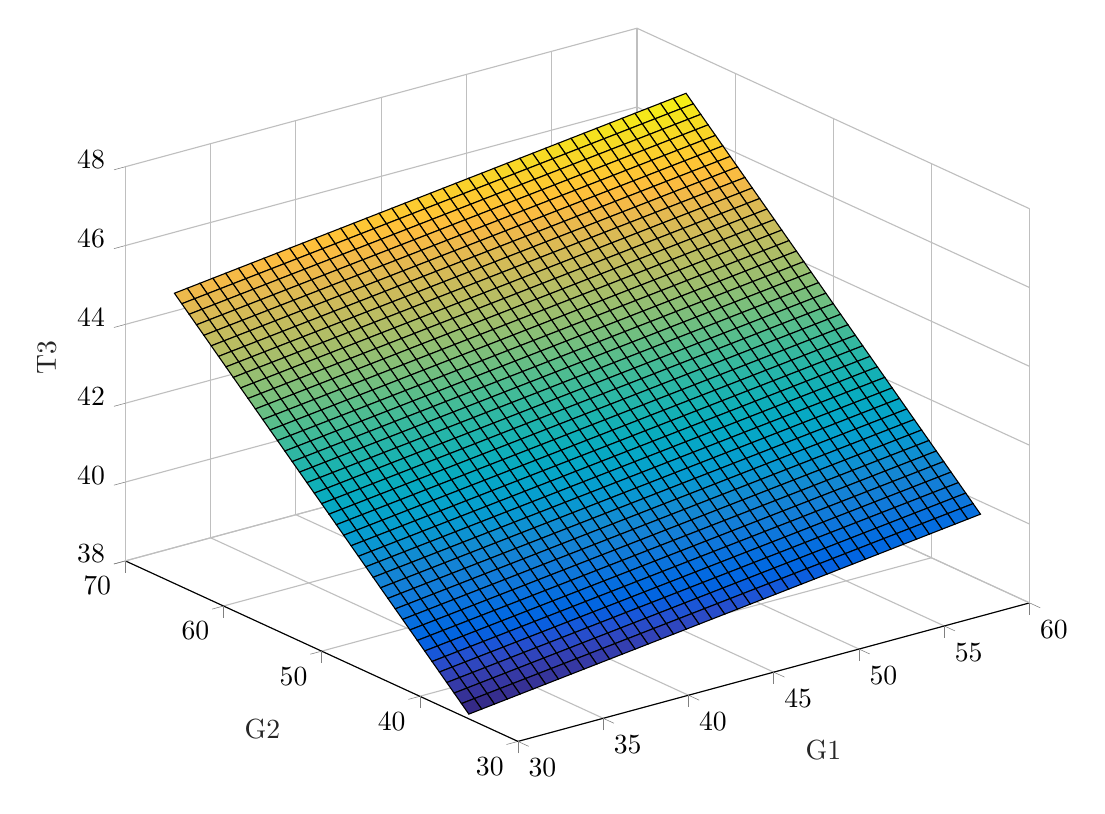
\begin{tikzpicture}

\begin{axis}[%
width=4.521in,
height=3.566in,
at={(0.758in,0.481in)},
scale only axis,
xmin=30,
xmax=60,
tick align=outside,
xlabel style={font=\color{white!15!black}},
xlabel={G1},
ymin=30,
ymax=70,
ylabel style={font=\color{white!15!black}},
ylabel={G2},
zmin=38,
zmax=48,
zlabel style={font=\color{white!15!black}},
zlabel={T3},
view={-37.5}{30},
axis background/.style={fill=white},
axis x line*=bottom,
axis y line*=left,
axis z line*=left,
xmajorgrids,
ymajorgrids,
zmajorgrids
]

\addplot3[%
surf,
shader=flat corner, draw=black, z buffer=sort, colormap={mymap}{[1pt] rgb(0pt)=(0.2081,0.1663,0.5292); rgb(1pt)=(0.211624,0.189781,0.577676); rgb(2pt)=(0.212252,0.213771,0.626971); rgb(3pt)=(0.2081,0.2386,0.677086); rgb(4pt)=(0.195905,0.264457,0.7279); rgb(5pt)=(0.170729,0.291938,0.779248); rgb(6pt)=(0.125271,0.324243,0.830271); rgb(7pt)=(0.0591333,0.359833,0.868333); rgb(8pt)=(0.0116952,0.38751,0.881957); rgb(9pt)=(0.00595714,0.408614,0.882843); rgb(10pt)=(0.0165143,0.4266,0.878633); rgb(11pt)=(0.0328524,0.443043,0.871957); rgb(12pt)=(0.0498143,0.458571,0.864057); rgb(13pt)=(0.0629333,0.47369,0.855438); rgb(14pt)=(0.0722667,0.488667,0.8467); rgb(15pt)=(0.0779429,0.503986,0.838371); rgb(16pt)=(0.0793476,0.520024,0.831181); rgb(17pt)=(0.0749429,0.537543,0.826271); rgb(18pt)=(0.0640571,0.556986,0.823957); rgb(19pt)=(0.0487714,0.577224,0.822829); rgb(20pt)=(0.0343429,0.596581,0.819852); rgb(21pt)=(0.0265,0.6137,0.8135); rgb(22pt)=(0.0238905,0.628662,0.803762); rgb(23pt)=(0.0230905,0.641786,0.791267); rgb(24pt)=(0.0227714,0.653486,0.776757); rgb(25pt)=(0.0266619,0.664195,0.760719); rgb(26pt)=(0.0383714,0.674271,0.743552); rgb(27pt)=(0.0589714,0.683757,0.725386); rgb(28pt)=(0.0843,0.692833,0.706167); rgb(29pt)=(0.113295,0.7015,0.685857); rgb(30pt)=(0.145271,0.709757,0.664629); rgb(31pt)=(0.180133,0.717657,0.642433); rgb(32pt)=(0.217829,0.725043,0.619262); rgb(33pt)=(0.258643,0.731714,0.595429); rgb(34pt)=(0.302171,0.737605,0.571186); rgb(35pt)=(0.348167,0.742433,0.547267); rgb(36pt)=(0.395257,0.7459,0.524443); rgb(37pt)=(0.44201,0.748081,0.503314); rgb(38pt)=(0.487124,0.749062,0.483976); rgb(39pt)=(0.530029,0.749114,0.466114); rgb(40pt)=(0.570857,0.748519,0.44939); rgb(41pt)=(0.609852,0.747314,0.433686); rgb(42pt)=(0.6473,0.7456,0.4188); rgb(43pt)=(0.683419,0.743476,0.404433); rgb(44pt)=(0.71841,0.741133,0.390476); rgb(45pt)=(0.752486,0.7384,0.376814); rgb(46pt)=(0.785843,0.735567,0.363271); rgb(47pt)=(0.818505,0.732733,0.34979); rgb(48pt)=(0.850657,0.7299,0.336029); rgb(49pt)=(0.882433,0.727433,0.3217); rgb(50pt)=(0.913933,0.725786,0.306276); rgb(51pt)=(0.944957,0.726114,0.288643); rgb(52pt)=(0.973895,0.731395,0.266648); rgb(53pt)=(0.993771,0.745457,0.240348); rgb(54pt)=(0.999043,0.765314,0.216414); rgb(55pt)=(0.995533,0.786057,0.196652); rgb(56pt)=(0.988,0.8066,0.179367); rgb(57pt)=(0.978857,0.827143,0.163314); rgb(58pt)=(0.9697,0.848138,0.147452); rgb(59pt)=(0.962586,0.870514,0.1309); rgb(60pt)=(0.958871,0.8949,0.113243); rgb(61pt)=(0.959824,0.921833,0.0948381); rgb(62pt)=(0.9661,0.951443,0.0755333); rgb(63pt)=(0.9763,0.9831,0.0538)}, mesh/rows=41]
table[row sep=crcr, point meta=\thisrow{c}] {%
%
x	y	z	c\\
30	35	38.12	38.12\\
30	35.75	38.30108	38.30108\\
30	36.5	38.48216	38.48216\\
30	37.25	38.66324	38.66324\\
30	38	38.84432	38.84432\\
30	38.75	39.0254	39.0254\\
30	39.5	39.20648	39.20648\\
30	40.25	39.38756	39.38756\\
30	41	39.56864	39.56864\\
30	41.75	39.74972	39.74972\\
30	42.5	39.9308	39.9308\\
30	43.25	40.11188	40.11188\\
30	44	40.29296	40.29296\\
30	44.75	40.47404	40.47404\\
30	45.5	40.65512	40.65512\\
30	46.25	40.8362	40.8362\\
30	47	41.01728	41.01728\\
30	47.75	41.19836	41.19836\\
30	48.5	41.37944	41.37944\\
30	49.25	41.56052	41.56052\\
30	50	41.7416	41.7416\\
30	50.75	41.92268	41.92268\\
30	51.5	42.10376	42.10376\\
30	52.25	42.28484	42.28484\\
30	53	42.46592	42.46592\\
30	53.75	42.647	42.647\\
30	54.5	42.82808	42.82808\\
30	55.25	43.00916	43.00916\\
30	56	43.19024	43.19024\\
30	56.75	43.37132	43.37132\\
30	57.5	43.5524	43.5524\\
30	58.25	43.73348	43.73348\\
30	59	43.91456	43.91456\\
30	59.75	44.09564	44.09564\\
30	60.5	44.27672	44.27672\\
30	61.25	44.4578	44.4578\\
30	62	44.63888	44.63888\\
30	62.75	44.81996	44.81996\\
30	63.5	45.00104	45.00104\\
30	64.25	45.18212	45.18212\\
30	65	45.3632	45.3632\\
30.75	35	38.158952	38.158952\\
30.75	35.75	38.340032	38.340032\\
30.75	36.5	38.521112	38.521112\\
30.75	37.25	38.702192	38.702192\\
30.75	38	38.883272	38.883272\\
30.75	38.75	39.064352	39.064352\\
30.75	39.5	39.245432	39.245432\\
30.75	40.25	39.426512	39.426512\\
30.75	41	39.607592	39.607592\\
30.75	41.75	39.788672	39.788672\\
30.75	42.5	39.969752	39.969752\\
30.75	43.25	40.150832	40.150832\\
30.75	44	40.331912	40.331912\\
30.75	44.75	40.512992	40.512992\\
30.75	45.5	40.694072	40.694072\\
30.75	46.25	40.875152	40.875152\\
30.75	47	41.056232	41.056232\\
30.75	47.75	41.237312	41.237312\\
30.75	48.5	41.418392	41.418392\\
30.75	49.25	41.599472	41.599472\\
30.75	50	41.780552	41.780552\\
30.75	50.75	41.961632	41.961632\\
30.75	51.5	42.142712	42.142712\\
30.75	52.25	42.323792	42.323792\\
30.75	53	42.504872	42.504872\\
30.75	53.75	42.685952	42.685952\\
30.75	54.5	42.867032	42.867032\\
30.75	55.25	43.048112	43.048112\\
30.75	56	43.229192	43.229192\\
30.75	56.75	43.410272	43.410272\\
30.75	57.5	43.591352	43.591352\\
30.75	58.25	43.772432	43.772432\\
30.75	59	43.953512	43.953512\\
30.75	59.75	44.134592	44.134592\\
30.75	60.5	44.315672	44.315672\\
30.75	61.25	44.496752	44.496752\\
30.75	62	44.677832	44.677832\\
30.75	62.75	44.858912	44.858912\\
30.75	63.5	45.039992	45.039992\\
30.75	64.25	45.221072	45.221072\\
30.75	65	45.402152	45.402152\\
31.5	35	38.197904	38.197904\\
31.5	35.75	38.378984	38.378984\\
31.5	36.5	38.560064	38.560064\\
31.5	37.25	38.741144	38.741144\\
31.5	38	38.922224	38.922224\\
31.5	38.75	39.103304	39.103304\\
31.5	39.5	39.284384	39.284384\\
31.5	40.25	39.465464	39.465464\\
31.5	41	39.646544	39.646544\\
31.5	41.75	39.827624	39.827624\\
31.5	42.5	40.008704	40.008704\\
31.5	43.25	40.189784	40.189784\\
31.5	44	40.370864	40.370864\\
31.5	44.75	40.551944	40.551944\\
31.5	45.5	40.733024	40.733024\\
31.5	46.25	40.914104	40.914104\\
31.5	47	41.095184	41.095184\\
31.5	47.75	41.276264	41.276264\\
31.5	48.5	41.457344	41.457344\\
31.5	49.25	41.638424	41.638424\\
31.5	50	41.819504	41.819504\\
31.5	50.75	42.000584	42.000584\\
31.5	51.5	42.181664	42.181664\\
31.5	52.25	42.362744	42.362744\\
31.5	53	42.543824	42.543824\\
31.5	53.75	42.724904	42.724904\\
31.5	54.5	42.905984	42.905984\\
31.5	55.25	43.087064	43.087064\\
31.5	56	43.268144	43.268144\\
31.5	56.75	43.449224	43.449224\\
31.5	57.5	43.630304	43.630304\\
31.5	58.25	43.811384	43.811384\\
31.5	59	43.992464	43.992464\\
31.5	59.75	44.173544	44.173544\\
31.5	60.5	44.354624	44.354624\\
31.5	61.25	44.535704	44.535704\\
31.5	62	44.716784	44.716784\\
31.5	62.75	44.897864	44.897864\\
31.5	63.5	45.078944	45.078944\\
31.5	64.25	45.260024	45.260024\\
31.5	65	45.441104	45.441104\\
32.25	35	38.236856	38.236856\\
32.25	35.75	38.417936	38.417936\\
32.25	36.5	38.599016	38.599016\\
32.25	37.25	38.780096	38.780096\\
32.25	38	38.961176	38.961176\\
32.25	38.75	39.142256	39.142256\\
32.25	39.5	39.323336	39.323336\\
32.25	40.25	39.504416	39.504416\\
32.25	41	39.685496	39.685496\\
32.25	41.75	39.866576	39.866576\\
32.25	42.5	40.047656	40.047656\\
32.25	43.25	40.228736	40.228736\\
32.25	44	40.409816	40.409816\\
32.25	44.75	40.590896	40.590896\\
32.25	45.5	40.771976	40.771976\\
32.25	46.25	40.953056	40.953056\\
32.25	47	41.134136	41.134136\\
32.25	47.75	41.315216	41.315216\\
32.25	48.5	41.496296	41.496296\\
32.25	49.25	41.677376	41.677376\\
32.25	50	41.858456	41.858456\\
32.25	50.75	42.039536	42.039536\\
32.25	51.5	42.220616	42.220616\\
32.25	52.25	42.401696	42.401696\\
32.25	53	42.582776	42.582776\\
32.25	53.75	42.763856	42.763856\\
32.25	54.5	42.944936	42.944936\\
32.25	55.25	43.126016	43.126016\\
32.25	56	43.307096	43.307096\\
32.25	56.75	43.488176	43.488176\\
32.25	57.5	43.669256	43.669256\\
32.25	58.25	43.850336	43.850336\\
32.25	59	44.031416	44.031416\\
32.25	59.75	44.212496	44.212496\\
32.25	60.5	44.393576	44.393576\\
32.25	61.25	44.574656	44.574656\\
32.25	62	44.755736	44.755736\\
32.25	62.75	44.936816	44.936816\\
32.25	63.5	45.117896	45.117896\\
32.25	64.25	45.298976	45.298976\\
32.25	65	45.480056	45.480056\\
33	35	38.275808	38.275808\\
33	35.75	38.456888	38.456888\\
33	36.5	38.637968	38.637968\\
33	37.25	38.819048	38.819048\\
33	38	39.000128	39.000128\\
33	38.75	39.181208	39.181208\\
33	39.5	39.362288	39.362288\\
33	40.25	39.543368	39.543368\\
33	41	39.724448	39.724448\\
33	41.75	39.905528	39.905528\\
33	42.5	40.086608	40.086608\\
33	43.25	40.267688	40.267688\\
33	44	40.448768	40.448768\\
33	44.75	40.629848	40.629848\\
33	45.5	40.810928	40.810928\\
33	46.25	40.992008	40.992008\\
33	47	41.173088	41.173088\\
33	47.75	41.354168	41.354168\\
33	48.5	41.535248	41.535248\\
33	49.25	41.716328	41.716328\\
33	50	41.897408	41.897408\\
33	50.75	42.078488	42.078488\\
33	51.5	42.259568	42.259568\\
33	52.25	42.440648	42.440648\\
33	53	42.621728	42.621728\\
33	53.75	42.802808	42.802808\\
33	54.5	42.983888	42.983888\\
33	55.25	43.164968	43.164968\\
33	56	43.346048	43.346048\\
33	56.75	43.527128	43.527128\\
33	57.5	43.708208	43.708208\\
33	58.25	43.889288	43.889288\\
33	59	44.070368	44.070368\\
33	59.75	44.251448	44.251448\\
33	60.5	44.432528	44.432528\\
33	61.25	44.613608	44.613608\\
33	62	44.794688	44.794688\\
33	62.75	44.975768	44.975768\\
33	63.5	45.156848	45.156848\\
33	64.25	45.337928	45.337928\\
33	65	45.519008	45.519008\\
33.75	35	38.31476	38.31476\\
33.75	35.75	38.49584	38.49584\\
33.75	36.5	38.67692	38.67692\\
33.75	37.25	38.858	38.858\\
33.75	38	39.03908	39.03908\\
33.75	38.75	39.22016	39.22016\\
33.75	39.5	39.40124	39.40124\\
33.75	40.25	39.58232	39.58232\\
33.75	41	39.7634	39.7634\\
33.75	41.75	39.94448	39.94448\\
33.75	42.5	40.12556	40.12556\\
33.75	43.25	40.30664	40.30664\\
33.75	44	40.48772	40.48772\\
33.75	44.75	40.6688	40.6688\\
33.75	45.5	40.84988	40.84988\\
33.75	46.25	41.03096	41.03096\\
33.75	47	41.21204	41.21204\\
33.75	47.75	41.39312	41.39312\\
33.75	48.5	41.5742	41.5742\\
33.75	49.25	41.75528	41.75528\\
33.75	50	41.93636	41.93636\\
33.75	50.75	42.11744	42.11744\\
33.75	51.5	42.29852	42.29852\\
33.75	52.25	42.4796	42.4796\\
33.75	53	42.66068	42.66068\\
33.75	53.75	42.84176	42.84176\\
33.75	54.5	43.02284	43.02284\\
33.75	55.25	43.20392	43.20392\\
33.75	56	43.385	43.385\\
33.75	56.75	43.56608	43.56608\\
33.75	57.5	43.74716	43.74716\\
33.75	58.25	43.92824	43.92824\\
33.75	59	44.10932	44.10932\\
33.75	59.75	44.2904	44.2904\\
33.75	60.5	44.47148	44.47148\\
33.75	61.25	44.65256	44.65256\\
33.75	62	44.83364	44.83364\\
33.75	62.75	45.01472	45.01472\\
33.75	63.5	45.1958	45.1958\\
33.75	64.25	45.37688	45.37688\\
33.75	65	45.55796	45.55796\\
34.5	35	38.353712	38.353712\\
34.5	35.75	38.534792	38.534792\\
34.5	36.5	38.715872	38.715872\\
34.5	37.25	38.896952	38.896952\\
34.5	38	39.078032	39.078032\\
34.5	38.75	39.259112	39.259112\\
34.5	39.5	39.440192	39.440192\\
34.5	40.25	39.621272	39.621272\\
34.5	41	39.802352	39.802352\\
34.5	41.75	39.983432	39.983432\\
34.5	42.5	40.164512	40.164512\\
34.5	43.25	40.345592	40.345592\\
34.5	44	40.526672	40.526672\\
34.5	44.75	40.707752	40.707752\\
34.5	45.5	40.888832	40.888832\\
34.5	46.25	41.069912	41.069912\\
34.5	47	41.250992	41.250992\\
34.5	47.75	41.432072	41.432072\\
34.5	48.5	41.613152	41.613152\\
34.5	49.25	41.794232	41.794232\\
34.5	50	41.975312	41.975312\\
34.5	50.75	42.156392	42.156392\\
34.5	51.5	42.337472	42.337472\\
34.5	52.25	42.518552	42.518552\\
34.5	53	42.699632	42.699632\\
34.5	53.75	42.880712	42.880712\\
34.5	54.5	43.061792	43.061792\\
34.5	55.25	43.242872	43.242872\\
34.5	56	43.423952	43.423952\\
34.5	56.75	43.605032	43.605032\\
34.5	57.5	43.786112	43.786112\\
34.5	58.25	43.967192	43.967192\\
34.5	59	44.148272	44.148272\\
34.5	59.75	44.329352	44.329352\\
34.5	60.5	44.510432	44.510432\\
34.5	61.25	44.691512	44.691512\\
34.5	62	44.872592	44.872592\\
34.5	62.75	45.053672	45.053672\\
34.5	63.5	45.234752	45.234752\\
34.5	64.25	45.415832	45.415832\\
34.5	65	45.596912	45.596912\\
35.25	35	38.392664	38.392664\\
35.25	35.75	38.573744	38.573744\\
35.25	36.5	38.754824	38.754824\\
35.25	37.25	38.935904	38.935904\\
35.25	38	39.116984	39.116984\\
35.25	38.75	39.298064	39.298064\\
35.25	39.5	39.479144	39.479144\\
35.25	40.25	39.660224	39.660224\\
35.25	41	39.841304	39.841304\\
35.25	41.75	40.022384	40.022384\\
35.25	42.5	40.203464	40.203464\\
35.25	43.25	40.384544	40.384544\\
35.25	44	40.565624	40.565624\\
35.25	44.75	40.746704	40.746704\\
35.25	45.5	40.927784	40.927784\\
35.25	46.25	41.108864	41.108864\\
35.25	47	41.289944	41.289944\\
35.25	47.75	41.471024	41.471024\\
35.25	48.5	41.652104	41.652104\\
35.25	49.25	41.833184	41.833184\\
35.25	50	42.014264	42.014264\\
35.25	50.75	42.195344	42.195344\\
35.25	51.5	42.376424	42.376424\\
35.25	52.25	42.557504	42.557504\\
35.25	53	42.738584	42.738584\\
35.25	53.75	42.919664	42.919664\\
35.25	54.5	43.100744	43.100744\\
35.25	55.25	43.281824	43.281824\\
35.25	56	43.462904	43.462904\\
35.25	56.75	43.643984	43.643984\\
35.25	57.5	43.825064	43.825064\\
35.25	58.25	44.006144	44.006144\\
35.25	59	44.187224	44.187224\\
35.25	59.75	44.368304	44.368304\\
35.25	60.5	44.549384	44.549384\\
35.25	61.25	44.730464	44.730464\\
35.25	62	44.911544	44.911544\\
35.25	62.75	45.092624	45.092624\\
35.25	63.5	45.273704	45.273704\\
35.25	64.25	45.454784	45.454784\\
35.25	65	45.635864	45.635864\\
36	35	38.431616	38.431616\\
36	35.75	38.612696	38.612696\\
36	36.5	38.793776	38.793776\\
36	37.25	38.974856	38.974856\\
36	38	39.155936	39.155936\\
36	38.75	39.337016	39.337016\\
36	39.5	39.518096	39.518096\\
36	40.25	39.699176	39.699176\\
36	41	39.880256	39.880256\\
36	41.75	40.061336	40.061336\\
36	42.5	40.242416	40.242416\\
36	43.25	40.423496	40.423496\\
36	44	40.604576	40.604576\\
36	44.75	40.785656	40.785656\\
36	45.5	40.966736	40.966736\\
36	46.25	41.147816	41.147816\\
36	47	41.328896	41.328896\\
36	47.75	41.509976	41.509976\\
36	48.5	41.691056	41.691056\\
36	49.25	41.872136	41.872136\\
36	50	42.053216	42.053216\\
36	50.75	42.234296	42.234296\\
36	51.5	42.415376	42.415376\\
36	52.25	42.596456	42.596456\\
36	53	42.777536	42.777536\\
36	53.75	42.958616	42.958616\\
36	54.5	43.139696	43.139696\\
36	55.25	43.320776	43.320776\\
36	56	43.501856	43.501856\\
36	56.75	43.682936	43.682936\\
36	57.5	43.864016	43.864016\\
36	58.25	44.045096	44.045096\\
36	59	44.226176	44.226176\\
36	59.75	44.407256	44.407256\\
36	60.5	44.588336	44.588336\\
36	61.25	44.769416	44.769416\\
36	62	44.950496	44.950496\\
36	62.75	45.131576	45.131576\\
36	63.5	45.312656	45.312656\\
36	64.25	45.493736	45.493736\\
36	65	45.674816	45.674816\\
36.75	35	38.470568	38.470568\\
36.75	35.75	38.651648	38.651648\\
36.75	36.5	38.832728	38.832728\\
36.75	37.25	39.013808	39.013808\\
36.75	38	39.194888	39.194888\\
36.75	38.75	39.375968	39.375968\\
36.75	39.5	39.557048	39.557048\\
36.75	40.25	39.738128	39.738128\\
36.75	41	39.919208	39.919208\\
36.75	41.75	40.100288	40.100288\\
36.75	42.5	40.281368	40.281368\\
36.75	43.25	40.462448	40.462448\\
36.75	44	40.643528	40.643528\\
36.75	44.75	40.824608	40.824608\\
36.75	45.5	41.005688	41.005688\\
36.75	46.25	41.186768	41.186768\\
36.75	47	41.367848	41.367848\\
36.75	47.75	41.548928	41.548928\\
36.75	48.5	41.730008	41.730008\\
36.75	49.25	41.911088	41.911088\\
36.75	50	42.092168	42.092168\\
36.75	50.75	42.273248	42.273248\\
36.75	51.5	42.454328	42.454328\\
36.75	52.25	42.635408	42.635408\\
36.75	53	42.816488	42.816488\\
36.75	53.75	42.997568	42.997568\\
36.75	54.5	43.178648	43.178648\\
36.75	55.25	43.359728	43.359728\\
36.75	56	43.540808	43.540808\\
36.75	56.75	43.721888	43.721888\\
36.75	57.5	43.902968	43.902968\\
36.75	58.25	44.084048	44.084048\\
36.75	59	44.265128	44.265128\\
36.75	59.75	44.446208	44.446208\\
36.75	60.5	44.627288	44.627288\\
36.75	61.25	44.808368	44.808368\\
36.75	62	44.989448	44.989448\\
36.75	62.75	45.170528	45.170528\\
36.75	63.5	45.351608	45.351608\\
36.75	64.25	45.532688	45.532688\\
36.75	65	45.713768	45.713768\\
37.5	35	38.50952	38.50952\\
37.5	35.75	38.6906	38.6906\\
37.5	36.5	38.87168	38.87168\\
37.5	37.25	39.05276	39.05276\\
37.5	38	39.23384	39.23384\\
37.5	38.75	39.41492	39.41492\\
37.5	39.5	39.596	39.596\\
37.5	40.25	39.77708	39.77708\\
37.5	41	39.95816	39.95816\\
37.5	41.75	40.13924	40.13924\\
37.5	42.5	40.32032	40.32032\\
37.5	43.25	40.5014	40.5014\\
37.5	44	40.68248	40.68248\\
37.5	44.75	40.86356	40.86356\\
37.5	45.5	41.04464	41.04464\\
37.5	46.25	41.22572	41.22572\\
37.5	47	41.4068	41.4068\\
37.5	47.75	41.58788	41.58788\\
37.5	48.5	41.76896	41.76896\\
37.5	49.25	41.95004	41.95004\\
37.5	50	42.13112	42.13112\\
37.5	50.75	42.3122	42.3122\\
37.5	51.5	42.49328	42.49328\\
37.5	52.25	42.67436	42.67436\\
37.5	53	42.85544	42.85544\\
37.5	53.75	43.03652	43.03652\\
37.5	54.5	43.2176	43.2176\\
37.5	55.25	43.39868	43.39868\\
37.5	56	43.57976	43.57976\\
37.5	56.75	43.76084	43.76084\\
37.5	57.5	43.94192	43.94192\\
37.5	58.25	44.123	44.123\\
37.5	59	44.30408	44.30408\\
37.5	59.75	44.48516	44.48516\\
37.5	60.5	44.66624	44.66624\\
37.5	61.25	44.84732	44.84732\\
37.5	62	45.0284	45.0284\\
37.5	62.75	45.20948	45.20948\\
37.5	63.5	45.39056	45.39056\\
37.5	64.25	45.57164	45.57164\\
37.5	65	45.75272	45.75272\\
38.25	35	38.548472	38.548472\\
38.25	35.75	38.729552	38.729552\\
38.25	36.5	38.910632	38.910632\\
38.25	37.25	39.091712	39.091712\\
38.25	38	39.272792	39.272792\\
38.25	38.75	39.453872	39.453872\\
38.25	39.5	39.634952	39.634952\\
38.25	40.25	39.816032	39.816032\\
38.25	41	39.997112	39.997112\\
38.25	41.75	40.178192	40.178192\\
38.25	42.5	40.359272	40.359272\\
38.25	43.25	40.540352	40.540352\\
38.25	44	40.721432	40.721432\\
38.25	44.75	40.902512	40.902512\\
38.25	45.5	41.083592	41.083592\\
38.25	46.25	41.264672	41.264672\\
38.25	47	41.445752	41.445752\\
38.25	47.75	41.626832	41.626832\\
38.25	48.5	41.807912	41.807912\\
38.25	49.25	41.988992	41.988992\\
38.25	50	42.170072	42.170072\\
38.25	50.75	42.351152	42.351152\\
38.25	51.5	42.532232	42.532232\\
38.25	52.25	42.713312	42.713312\\
38.25	53	42.894392	42.894392\\
38.25	53.75	43.075472	43.075472\\
38.25	54.5	43.256552	43.256552\\
38.25	55.25	43.437632	43.437632\\
38.25	56	43.618712	43.618712\\
38.25	56.75	43.799792	43.799792\\
38.25	57.5	43.980872	43.980872\\
38.25	58.25	44.161952	44.161952\\
38.25	59	44.343032	44.343032\\
38.25	59.75	44.524112	44.524112\\
38.25	60.5	44.705192	44.705192\\
38.25	61.25	44.886272	44.886272\\
38.25	62	45.067352	45.067352\\
38.25	62.75	45.248432	45.248432\\
38.25	63.5	45.429512	45.429512\\
38.25	64.25	45.610592	45.610592\\
38.25	65	45.791672	45.791672\\
39	35	38.587424	38.587424\\
39	35.75	38.768504	38.768504\\
39	36.5	38.949584	38.949584\\
39	37.25	39.130664	39.130664\\
39	38	39.311744	39.311744\\
39	38.75	39.492824	39.492824\\
39	39.5	39.673904	39.673904\\
39	40.25	39.854984	39.854984\\
39	41	40.036064	40.036064\\
39	41.75	40.217144	40.217144\\
39	42.5	40.398224	40.398224\\
39	43.25	40.579304	40.579304\\
39	44	40.760384	40.760384\\
39	44.75	40.941464	40.941464\\
39	45.5	41.122544	41.122544\\
39	46.25	41.303624	41.303624\\
39	47	41.484704	41.484704\\
39	47.75	41.665784	41.665784\\
39	48.5	41.846864	41.846864\\
39	49.25	42.027944	42.027944\\
39	50	42.209024	42.209024\\
39	50.75	42.390104	42.390104\\
39	51.5	42.571184	42.571184\\
39	52.25	42.752264	42.752264\\
39	53	42.933344	42.933344\\
39	53.75	43.114424	43.114424\\
39	54.5	43.295504	43.295504\\
39	55.25	43.476584	43.476584\\
39	56	43.657664	43.657664\\
39	56.75	43.838744	43.838744\\
39	57.5	44.019824	44.019824\\
39	58.25	44.200904	44.200904\\
39	59	44.381984	44.381984\\
39	59.75	44.563064	44.563064\\
39	60.5	44.744144	44.744144\\
39	61.25	44.925224	44.925224\\
39	62	45.106304	45.106304\\
39	62.75	45.287384	45.287384\\
39	63.5	45.468464	45.468464\\
39	64.25	45.649544	45.649544\\
39	65	45.830624	45.830624\\
39.75	35	38.626376	38.626376\\
39.75	35.75	38.807456	38.807456\\
39.75	36.5	38.988536	38.988536\\
39.75	37.25	39.169616	39.169616\\
39.75	38	39.350696	39.350696\\
39.75	38.75	39.531776	39.531776\\
39.75	39.5	39.712856	39.712856\\
39.75	40.25	39.893936	39.893936\\
39.75	41	40.075016	40.075016\\
39.75	41.75	40.256096	40.256096\\
39.75	42.5	40.437176	40.437176\\
39.75	43.25	40.618256	40.618256\\
39.75	44	40.799336	40.799336\\
39.75	44.75	40.980416	40.980416\\
39.75	45.5	41.161496	41.161496\\
39.75	46.25	41.342576	41.342576\\
39.75	47	41.523656	41.523656\\
39.75	47.75	41.704736	41.704736\\
39.75	48.5	41.885816	41.885816\\
39.75	49.25	42.066896	42.066896\\
39.75	50	42.247976	42.247976\\
39.75	50.75	42.429056	42.429056\\
39.75	51.5	42.610136	42.610136\\
39.75	52.25	42.791216	42.791216\\
39.75	53	42.972296	42.972296\\
39.75	53.75	43.153376	43.153376\\
39.75	54.5	43.334456	43.334456\\
39.75	55.25	43.515536	43.515536\\
39.75	56	43.696616	43.696616\\
39.75	56.75	43.877696	43.877696\\
39.75	57.5	44.058776	44.058776\\
39.75	58.25	44.239856	44.239856\\
39.75	59	44.420936	44.420936\\
39.75	59.75	44.602016	44.602016\\
39.75	60.5	44.783096	44.783096\\
39.75	61.25	44.964176	44.964176\\
39.75	62	45.145256	45.145256\\
39.75	62.75	45.326336	45.326336\\
39.75	63.5	45.507416	45.507416\\
39.75	64.25	45.688496	45.688496\\
39.75	65	45.869576	45.869576\\
40.5	35	38.665328	38.665328\\
40.5	35.75	38.846408	38.846408\\
40.5	36.5	39.027488	39.027488\\
40.5	37.25	39.208568	39.208568\\
40.5	38	39.389648	39.389648\\
40.5	38.75	39.570728	39.570728\\
40.5	39.5	39.751808	39.751808\\
40.5	40.25	39.932888	39.932888\\
40.5	41	40.113968	40.113968\\
40.5	41.75	40.295048	40.295048\\
40.5	42.5	40.476128	40.476128\\
40.5	43.25	40.657208	40.657208\\
40.5	44	40.838288	40.838288\\
40.5	44.75	41.019368	41.019368\\
40.5	45.5	41.200448	41.200448\\
40.5	46.25	41.381528	41.381528\\
40.5	47	41.562608	41.562608\\
40.5	47.75	41.743688	41.743688\\
40.5	48.5	41.924768	41.924768\\
40.5	49.25	42.105848	42.105848\\
40.5	50	42.286928	42.286928\\
40.5	50.75	42.468008	42.468008\\
40.5	51.5	42.649088	42.649088\\
40.5	52.25	42.830168	42.830168\\
40.5	53	43.011248	43.011248\\
40.5	53.75	43.192328	43.192328\\
40.5	54.5	43.373408	43.373408\\
40.5	55.25	43.554488	43.554488\\
40.5	56	43.735568	43.735568\\
40.5	56.75	43.916648	43.916648\\
40.5	57.5	44.097728	44.097728\\
40.5	58.25	44.278808	44.278808\\
40.5	59	44.459888	44.459888\\
40.5	59.75	44.640968	44.640968\\
40.5	60.5	44.822048	44.822048\\
40.5	61.25	45.003128	45.003128\\
40.5	62	45.184208	45.184208\\
40.5	62.75	45.365288	45.365288\\
40.5	63.5	45.546368	45.546368\\
40.5	64.25	45.727448	45.727448\\
40.5	65	45.908528	45.908528\\
41.25	35	38.70428	38.70428\\
41.25	35.75	38.88536	38.88536\\
41.25	36.5	39.06644	39.06644\\
41.25	37.25	39.24752	39.24752\\
41.25	38	39.4286	39.4286\\
41.25	38.75	39.60968	39.60968\\
41.25	39.5	39.79076	39.79076\\
41.25	40.25	39.97184	39.97184\\
41.25	41	40.15292	40.15292\\
41.25	41.75	40.334	40.334\\
41.25	42.5	40.51508	40.51508\\
41.25	43.25	40.69616	40.69616\\
41.25	44	40.87724	40.87724\\
41.25	44.75	41.05832	41.05832\\
41.25	45.5	41.2394	41.2394\\
41.25	46.25	41.42048	41.42048\\
41.25	47	41.60156	41.60156\\
41.25	47.75	41.78264	41.78264\\
41.25	48.5	41.96372	41.96372\\
41.25	49.25	42.1448	42.1448\\
41.25	50	42.32588	42.32588\\
41.25	50.75	42.50696	42.50696\\
41.25	51.5	42.68804	42.68804\\
41.25	52.25	42.86912	42.86912\\
41.25	53	43.0502	43.0502\\
41.25	53.75	43.23128	43.23128\\
41.25	54.5	43.41236	43.41236\\
41.25	55.25	43.59344	43.59344\\
41.25	56	43.77452	43.77452\\
41.25	56.75	43.9556	43.9556\\
41.25	57.5	44.13668	44.13668\\
41.25	58.25	44.31776	44.31776\\
41.25	59	44.49884	44.49884\\
41.25	59.75	44.67992	44.67992\\
41.25	60.5	44.861	44.861\\
41.25	61.25	45.04208	45.04208\\
41.25	62	45.22316	45.22316\\
41.25	62.75	45.40424	45.40424\\
41.25	63.5	45.58532	45.58532\\
41.25	64.25	45.7664	45.7664\\
41.25	65	45.94748	45.94748\\
42	35	38.743232	38.743232\\
42	35.75	38.924312	38.924312\\
42	36.5	39.105392	39.105392\\
42	37.25	39.286472	39.286472\\
42	38	39.467552	39.467552\\
42	38.75	39.648632	39.648632\\
42	39.5	39.829712	39.829712\\
42	40.25	40.010792	40.010792\\
42	41	40.191872	40.191872\\
42	41.75	40.372952	40.372952\\
42	42.5	40.554032	40.554032\\
42	43.25	40.735112	40.735112\\
42	44	40.916192	40.916192\\
42	44.75	41.097272	41.097272\\
42	45.5	41.278352	41.278352\\
42	46.25	41.459432	41.459432\\
42	47	41.640512	41.640512\\
42	47.75	41.821592	41.821592\\
42	48.5	42.002672	42.002672\\
42	49.25	42.183752	42.183752\\
42	50	42.364832	42.364832\\
42	50.75	42.545912	42.545912\\
42	51.5	42.726992	42.726992\\
42	52.25	42.908072	42.908072\\
42	53	43.089152	43.089152\\
42	53.75	43.270232	43.270232\\
42	54.5	43.451312	43.451312\\
42	55.25	43.632392	43.632392\\
42	56	43.813472	43.813472\\
42	56.75	43.994552	43.994552\\
42	57.5	44.175632	44.175632\\
42	58.25	44.356712	44.356712\\
42	59	44.537792	44.537792\\
42	59.75	44.718872	44.718872\\
42	60.5	44.899952	44.899952\\
42	61.25	45.081032	45.081032\\
42	62	45.262112	45.262112\\
42	62.75	45.443192	45.443192\\
42	63.5	45.624272	45.624272\\
42	64.25	45.805352	45.805352\\
42	65	45.986432	45.986432\\
42.75	35	38.782184	38.782184\\
42.75	35.75	38.963264	38.963264\\
42.75	36.5	39.144344	39.144344\\
42.75	37.25	39.325424	39.325424\\
42.75	38	39.506504	39.506504\\
42.75	38.75	39.687584	39.687584\\
42.75	39.5	39.868664	39.868664\\
42.75	40.25	40.049744	40.049744\\
42.75	41	40.230824	40.230824\\
42.75	41.75	40.411904	40.411904\\
42.75	42.5	40.592984	40.592984\\
42.75	43.25	40.774064	40.774064\\
42.75	44	40.955144	40.955144\\
42.75	44.75	41.136224	41.136224\\
42.75	45.5	41.317304	41.317304\\
42.75	46.25	41.498384	41.498384\\
42.75	47	41.679464	41.679464\\
42.75	47.75	41.860544	41.860544\\
42.75	48.5	42.041624	42.041624\\
42.75	49.25	42.222704	42.222704\\
42.75	50	42.403784	42.403784\\
42.75	50.75	42.584864	42.584864\\
42.75	51.5	42.765944	42.765944\\
42.75	52.25	42.947024	42.947024\\
42.75	53	43.128104	43.128104\\
42.75	53.75	43.309184	43.309184\\
42.75	54.5	43.490264	43.490264\\
42.75	55.25	43.671344	43.671344\\
42.75	56	43.852424	43.852424\\
42.75	56.75	44.033504	44.033504\\
42.75	57.5	44.214584	44.214584\\
42.75	58.25	44.395664	44.395664\\
42.75	59	44.576744	44.576744\\
42.75	59.75	44.757824	44.757824\\
42.75	60.5	44.938904	44.938904\\
42.75	61.25	45.119984	45.119984\\
42.75	62	45.301064	45.301064\\
42.75	62.75	45.482144	45.482144\\
42.75	63.5	45.663224	45.663224\\
42.75	64.25	45.844304	45.844304\\
42.75	65	46.025384	46.025384\\
43.5	35	38.821136	38.821136\\
43.5	35.75	39.002216	39.002216\\
43.5	36.5	39.183296	39.183296\\
43.5	37.25	39.364376	39.364376\\
43.5	38	39.545456	39.545456\\
43.5	38.75	39.726536	39.726536\\
43.5	39.5	39.907616	39.907616\\
43.5	40.25	40.088696	40.088696\\
43.5	41	40.269776	40.269776\\
43.5	41.75	40.450856	40.450856\\
43.5	42.5	40.631936	40.631936\\
43.5	43.25	40.813016	40.813016\\
43.5	44	40.994096	40.994096\\
43.5	44.75	41.175176	41.175176\\
43.5	45.5	41.356256	41.356256\\
43.5	46.25	41.537336	41.537336\\
43.5	47	41.718416	41.718416\\
43.5	47.75	41.899496	41.899496\\
43.5	48.5	42.080576	42.080576\\
43.5	49.25	42.261656	42.261656\\
43.5	50	42.442736	42.442736\\
43.5	50.75	42.623816	42.623816\\
43.5	51.5	42.804896	42.804896\\
43.5	52.25	42.985976	42.985976\\
43.5	53	43.167056	43.167056\\
43.5	53.75	43.348136	43.348136\\
43.5	54.5	43.529216	43.529216\\
43.5	55.25	43.710296	43.710296\\
43.5	56	43.891376	43.891376\\
43.5	56.75	44.072456	44.072456\\
43.5	57.5	44.253536	44.253536\\
43.5	58.25	44.434616	44.434616\\
43.5	59	44.615696	44.615696\\
43.5	59.75	44.796776	44.796776\\
43.5	60.5	44.977856	44.977856\\
43.5	61.25	45.158936	45.158936\\
43.5	62	45.340016	45.340016\\
43.5	62.75	45.521096	45.521096\\
43.5	63.5	45.702176	45.702176\\
43.5	64.25	45.883256	45.883256\\
43.5	65	46.064336	46.064336\\
44.25	35	38.860088	38.860088\\
44.25	35.75	39.041168	39.041168\\
44.25	36.5	39.222248	39.222248\\
44.25	37.25	39.403328	39.403328\\
44.25	38	39.584408	39.584408\\
44.25	38.75	39.765488	39.765488\\
44.25	39.5	39.946568	39.946568\\
44.25	40.25	40.127648	40.127648\\
44.25	41	40.308728	40.308728\\
44.25	41.75	40.489808	40.489808\\
44.25	42.5	40.670888	40.670888\\
44.25	43.25	40.851968	40.851968\\
44.25	44	41.033048	41.033048\\
44.25	44.75	41.214128	41.214128\\
44.25	45.5	41.395208	41.395208\\
44.25	46.25	41.576288	41.576288\\
44.25	47	41.757368	41.757368\\
44.25	47.75	41.938448	41.938448\\
44.25	48.5	42.119528	42.119528\\
44.25	49.25	42.300608	42.300608\\
44.25	50	42.481688	42.481688\\
44.25	50.75	42.662768	42.662768\\
44.25	51.5	42.843848	42.843848\\
44.25	52.25	43.024928	43.024928\\
44.25	53	43.206008	43.206008\\
44.25	53.75	43.387088	43.387088\\
44.25	54.5	43.568168	43.568168\\
44.25	55.25	43.749248	43.749248\\
44.25	56	43.930328	43.930328\\
44.25	56.75	44.111408	44.111408\\
44.25	57.5	44.292488	44.292488\\
44.25	58.25	44.473568	44.473568\\
44.25	59	44.654648	44.654648\\
44.25	59.75	44.835728	44.835728\\
44.25	60.5	45.016808	45.016808\\
44.25	61.25	45.197888	45.197888\\
44.25	62	45.378968	45.378968\\
44.25	62.75	45.560048	45.560048\\
44.25	63.5	45.741128	45.741128\\
44.25	64.25	45.922208	45.922208\\
44.25	65	46.103288	46.103288\\
45	35	38.89904	38.89904\\
45	35.75	39.08012	39.08012\\
45	36.5	39.2612	39.2612\\
45	37.25	39.44228	39.44228\\
45	38	39.62336	39.62336\\
45	38.75	39.80444	39.80444\\
45	39.5	39.98552	39.98552\\
45	40.25	40.1666	40.1666\\
45	41	40.34768	40.34768\\
45	41.75	40.52876	40.52876\\
45	42.5	40.70984	40.70984\\
45	43.25	40.89092	40.89092\\
45	44	41.072	41.072\\
45	44.75	41.25308	41.25308\\
45	45.5	41.43416	41.43416\\
45	46.25	41.61524	41.61524\\
45	47	41.79632	41.79632\\
45	47.75	41.9774	41.9774\\
45	48.5	42.15848	42.15848\\
45	49.25	42.33956	42.33956\\
45	50	42.52064	42.52064\\
45	50.75	42.70172	42.70172\\
45	51.5	42.8828	42.8828\\
45	52.25	43.06388	43.06388\\
45	53	43.24496	43.24496\\
45	53.75	43.42604	43.42604\\
45	54.5	43.60712	43.60712\\
45	55.25	43.7882	43.7882\\
45	56	43.96928	43.96928\\
45	56.75	44.15036	44.15036\\
45	57.5	44.33144	44.33144\\
45	58.25	44.51252	44.51252\\
45	59	44.6936	44.6936\\
45	59.75	44.87468	44.87468\\
45	60.5	45.05576	45.05576\\
45	61.25	45.23684	45.23684\\
45	62	45.41792	45.41792\\
45	62.75	45.599	45.599\\
45	63.5	45.78008	45.78008\\
45	64.25	45.96116	45.96116\\
45	65	46.14224	46.14224\\
45.75	35	38.937992	38.937992\\
45.75	35.75	39.119072	39.119072\\
45.75	36.5	39.300152	39.300152\\
45.75	37.25	39.481232	39.481232\\
45.75	38	39.662312	39.662312\\
45.75	38.75	39.843392	39.843392\\
45.75	39.5	40.024472	40.024472\\
45.75	40.25	40.205552	40.205552\\
45.75	41	40.386632	40.386632\\
45.75	41.75	40.567712	40.567712\\
45.75	42.5	40.748792	40.748792\\
45.75	43.25	40.929872	40.929872\\
45.75	44	41.110952	41.110952\\
45.75	44.75	41.292032	41.292032\\
45.75	45.5	41.473112	41.473112\\
45.75	46.25	41.654192	41.654192\\
45.75	47	41.835272	41.835272\\
45.75	47.75	42.016352	42.016352\\
45.75	48.5	42.197432	42.197432\\
45.75	49.25	42.378512	42.378512\\
45.75	50	42.559592	42.559592\\
45.75	50.75	42.740672	42.740672\\
45.75	51.5	42.921752	42.921752\\
45.75	52.25	43.102832	43.102832\\
45.75	53	43.283912	43.283912\\
45.75	53.75	43.464992	43.464992\\
45.75	54.5	43.646072	43.646072\\
45.75	55.25	43.827152	43.827152\\
45.75	56	44.008232	44.008232\\
45.75	56.75	44.189312	44.189312\\
45.75	57.5	44.370392	44.370392\\
45.75	58.25	44.551472	44.551472\\
45.75	59	44.732552	44.732552\\
45.75	59.75	44.913632	44.913632\\
45.75	60.5	45.094712	45.094712\\
45.75	61.25	45.275792	45.275792\\
45.75	62	45.456872	45.456872\\
45.75	62.75	45.637952	45.637952\\
45.75	63.5	45.819032	45.819032\\
45.75	64.25	46.000112	46.000112\\
45.75	65	46.181192	46.181192\\
46.5	35	38.976944	38.976944\\
46.5	35.75	39.158024	39.158024\\
46.5	36.5	39.339104	39.339104\\
46.5	37.25	39.520184	39.520184\\
46.5	38	39.701264	39.701264\\
46.5	38.75	39.882344	39.882344\\
46.5	39.5	40.063424	40.063424\\
46.5	40.25	40.244504	40.244504\\
46.5	41	40.425584	40.425584\\
46.5	41.75	40.606664	40.606664\\
46.5	42.5	40.787744	40.787744\\
46.5	43.25	40.968824	40.968824\\
46.5	44	41.149904	41.149904\\
46.5	44.75	41.330984	41.330984\\
46.5	45.5	41.512064	41.512064\\
46.5	46.25	41.693144	41.693144\\
46.5	47	41.874224	41.874224\\
46.5	47.75	42.055304	42.055304\\
46.5	48.5	42.236384	42.236384\\
46.5	49.25	42.417464	42.417464\\
46.5	50	42.598544	42.598544\\
46.5	50.75	42.779624	42.779624\\
46.5	51.5	42.960704	42.960704\\
46.5	52.25	43.141784	43.141784\\
46.5	53	43.322864	43.322864\\
46.5	53.75	43.503944	43.503944\\
46.5	54.5	43.685024	43.685024\\
46.5	55.25	43.866104	43.866104\\
46.5	56	44.047184	44.047184\\
46.5	56.75	44.228264	44.228264\\
46.5	57.5	44.409344	44.409344\\
46.5	58.25	44.590424	44.590424\\
46.5	59	44.771504	44.771504\\
46.5	59.75	44.952584	44.952584\\
46.5	60.5	45.133664	45.133664\\
46.5	61.25	45.314744	45.314744\\
46.5	62	45.495824	45.495824\\
46.5	62.75	45.676904	45.676904\\
46.5	63.5	45.857984	45.857984\\
46.5	64.25	46.039064	46.039064\\
46.5	65	46.220144	46.220144\\
47.25	35	39.015896	39.015896\\
47.25	35.75	39.196976	39.196976\\
47.25	36.5	39.378056	39.378056\\
47.25	37.25	39.559136	39.559136\\
47.25	38	39.740216	39.740216\\
47.25	38.75	39.921296	39.921296\\
47.25	39.5	40.102376	40.102376\\
47.25	40.25	40.283456	40.283456\\
47.25	41	40.464536	40.464536\\
47.25	41.75	40.645616	40.645616\\
47.25	42.5	40.826696	40.826696\\
47.25	43.25	41.007776	41.007776\\
47.25	44	41.188856	41.188856\\
47.25	44.75	41.369936	41.369936\\
47.25	45.5	41.551016	41.551016\\
47.25	46.25	41.732096	41.732096\\
47.25	47	41.913176	41.913176\\
47.25	47.75	42.094256	42.094256\\
47.25	48.5	42.275336	42.275336\\
47.25	49.25	42.456416	42.456416\\
47.25	50	42.637496	42.637496\\
47.25	50.75	42.818576	42.818576\\
47.25	51.5	42.999656	42.999656\\
47.25	52.25	43.180736	43.180736\\
47.25	53	43.361816	43.361816\\
47.25	53.75	43.542896	43.542896\\
47.25	54.5	43.723976	43.723976\\
47.25	55.25	43.905056	43.905056\\
47.25	56	44.086136	44.086136\\
47.25	56.75	44.267216	44.267216\\
47.25	57.5	44.448296	44.448296\\
47.25	58.25	44.629376	44.629376\\
47.25	59	44.810456	44.810456\\
47.25	59.75	44.991536	44.991536\\
47.25	60.5	45.172616	45.172616\\
47.25	61.25	45.353696	45.353696\\
47.25	62	45.534776	45.534776\\
47.25	62.75	45.715856	45.715856\\
47.25	63.5	45.896936	45.896936\\
47.25	64.25	46.078016	46.078016\\
47.25	65	46.259096	46.259096\\
48	35	39.054848	39.054848\\
48	35.75	39.235928	39.235928\\
48	36.5	39.417008	39.417008\\
48	37.25	39.598088	39.598088\\
48	38	39.779168	39.779168\\
48	38.75	39.960248	39.960248\\
48	39.5	40.141328	40.141328\\
48	40.25	40.322408	40.322408\\
48	41	40.503488	40.503488\\
48	41.75	40.684568	40.684568\\
48	42.5	40.865648	40.865648\\
48	43.25	41.046728	41.046728\\
48	44	41.227808	41.227808\\
48	44.75	41.408888	41.408888\\
48	45.5	41.589968	41.589968\\
48	46.25	41.771048	41.771048\\
48	47	41.952128	41.952128\\
48	47.75	42.133208	42.133208\\
48	48.5	42.314288	42.314288\\
48	49.25	42.495368	42.495368\\
48	50	42.676448	42.676448\\
48	50.75	42.857528	42.857528\\
48	51.5	43.038608	43.038608\\
48	52.25	43.219688	43.219688\\
48	53	43.400768	43.400768\\
48	53.75	43.581848	43.581848\\
48	54.5	43.762928	43.762928\\
48	55.25	43.944008	43.944008\\
48	56	44.125088	44.125088\\
48	56.75	44.306168	44.306168\\
48	57.5	44.487248	44.487248\\
48	58.25	44.668328	44.668328\\
48	59	44.849408	44.849408\\
48	59.75	45.030488	45.030488\\
48	60.5	45.211568	45.211568\\
48	61.25	45.392648	45.392648\\
48	62	45.573728	45.573728\\
48	62.75	45.754808	45.754808\\
48	63.5	45.935888	45.935888\\
48	64.25	46.116968	46.116968\\
48	65	46.298048	46.298048\\
48.75	35	39.0938	39.0938\\
48.75	35.75	39.27488	39.27488\\
48.75	36.5	39.45596	39.45596\\
48.75	37.25	39.63704	39.63704\\
48.75	38	39.81812	39.81812\\
48.75	38.75	39.9992	39.9992\\
48.75	39.5	40.18028	40.18028\\
48.75	40.25	40.36136	40.36136\\
48.75	41	40.54244	40.54244\\
48.75	41.75	40.72352	40.72352\\
48.75	42.5	40.9046	40.9046\\
48.75	43.25	41.08568	41.08568\\
48.75	44	41.26676	41.26676\\
48.75	44.75	41.44784	41.44784\\
48.75	45.5	41.62892	41.62892\\
48.75	46.25	41.81	41.81\\
48.75	47	41.99108	41.99108\\
48.75	47.75	42.17216	42.17216\\
48.75	48.5	42.35324	42.35324\\
48.75	49.25	42.53432	42.53432\\
48.75	50	42.7154	42.7154\\
48.75	50.75	42.89648	42.89648\\
48.75	51.5	43.07756	43.07756\\
48.75	52.25	43.25864	43.25864\\
48.75	53	43.43972	43.43972\\
48.75	53.75	43.6208	43.6208\\
48.75	54.5	43.80188	43.80188\\
48.75	55.25	43.98296	43.98296\\
48.75	56	44.16404	44.16404\\
48.75	56.75	44.34512	44.34512\\
48.75	57.5	44.5262	44.5262\\
48.75	58.25	44.70728	44.70728\\
48.75	59	44.88836	44.88836\\
48.75	59.75	45.06944	45.06944\\
48.75	60.5	45.25052	45.25052\\
48.75	61.25	45.4316	45.4316\\
48.75	62	45.61268	45.61268\\
48.75	62.75	45.79376	45.79376\\
48.75	63.5	45.97484	45.97484\\
48.75	64.25	46.15592	46.15592\\
48.75	65	46.337	46.337\\
49.5	35	39.132752	39.132752\\
49.5	35.75	39.313832	39.313832\\
49.5	36.5	39.494912	39.494912\\
49.5	37.25	39.675992	39.675992\\
49.5	38	39.857072	39.857072\\
49.5	38.75	40.038152	40.038152\\
49.5	39.5	40.219232	40.219232\\
49.5	40.25	40.400312	40.400312\\
49.5	41	40.581392	40.581392\\
49.5	41.75	40.762472	40.762472\\
49.5	42.5	40.943552	40.943552\\
49.5	43.25	41.124632	41.124632\\
49.5	44	41.305712	41.305712\\
49.5	44.75	41.486792	41.486792\\
49.5	45.5	41.667872	41.667872\\
49.5	46.25	41.848952	41.848952\\
49.5	47	42.030032	42.030032\\
49.5	47.75	42.211112	42.211112\\
49.5	48.5	42.392192	42.392192\\
49.5	49.25	42.573272	42.573272\\
49.5	50	42.754352	42.754352\\
49.5	50.75	42.935432	42.935432\\
49.5	51.5	43.116512	43.116512\\
49.5	52.25	43.297592	43.297592\\
49.5	53	43.478672	43.478672\\
49.5	53.75	43.659752	43.659752\\
49.5	54.5	43.840832	43.840832\\
49.5	55.25	44.021912	44.021912\\
49.5	56	44.202992	44.202992\\
49.5	56.75	44.384072	44.384072\\
49.5	57.5	44.565152	44.565152\\
49.5	58.25	44.746232	44.746232\\
49.5	59	44.927312	44.927312\\
49.5	59.75	45.108392	45.108392\\
49.5	60.5	45.289472	45.289472\\
49.5	61.25	45.470552	45.470552\\
49.5	62	45.651632	45.651632\\
49.5	62.75	45.832712	45.832712\\
49.5	63.5	46.013792	46.013792\\
49.5	64.25	46.194872	46.194872\\
49.5	65	46.375952	46.375952\\
50.25	35	39.171704	39.171704\\
50.25	35.75	39.352784	39.352784\\
50.25	36.5	39.533864	39.533864\\
50.25	37.25	39.714944	39.714944\\
50.25	38	39.896024	39.896024\\
50.25	38.75	40.077104	40.077104\\
50.25	39.5	40.258184	40.258184\\
50.25	40.25	40.439264	40.439264\\
50.25	41	40.620344	40.620344\\
50.25	41.75	40.801424	40.801424\\
50.25	42.5	40.982504	40.982504\\
50.25	43.25	41.163584	41.163584\\
50.25	44	41.344664	41.344664\\
50.25	44.75	41.525744	41.525744\\
50.25	45.5	41.706824	41.706824\\
50.25	46.25	41.887904	41.887904\\
50.25	47	42.068984	42.068984\\
50.25	47.75	42.250064	42.250064\\
50.25	48.5	42.431144	42.431144\\
50.25	49.25	42.612224	42.612224\\
50.25	50	42.793304	42.793304\\
50.25	50.75	42.974384	42.974384\\
50.25	51.5	43.155464	43.155464\\
50.25	52.25	43.336544	43.336544\\
50.25	53	43.517624	43.517624\\
50.25	53.75	43.698704	43.698704\\
50.25	54.5	43.879784	43.879784\\
50.25	55.25	44.060864	44.060864\\
50.25	56	44.241944	44.241944\\
50.25	56.75	44.423024	44.423024\\
50.25	57.5	44.604104	44.604104\\
50.25	58.25	44.785184	44.785184\\
50.25	59	44.966264	44.966264\\
50.25	59.75	45.147344	45.147344\\
50.25	60.5	45.328424	45.328424\\
50.25	61.25	45.509504	45.509504\\
50.25	62	45.690584	45.690584\\
50.25	62.75	45.871664	45.871664\\
50.25	63.5	46.052744	46.052744\\
50.25	64.25	46.233824	46.233824\\
50.25	65	46.414904	46.414904\\
51	35	39.210656	39.210656\\
51	35.75	39.391736	39.391736\\
51	36.5	39.572816	39.572816\\
51	37.25	39.753896	39.753896\\
51	38	39.934976	39.934976\\
51	38.75	40.116056	40.116056\\
51	39.5	40.297136	40.297136\\
51	40.25	40.478216	40.478216\\
51	41	40.659296	40.659296\\
51	41.75	40.840376	40.840376\\
51	42.5	41.021456	41.021456\\
51	43.25	41.202536	41.202536\\
51	44	41.383616	41.383616\\
51	44.75	41.564696	41.564696\\
51	45.5	41.745776	41.745776\\
51	46.25	41.926856	41.926856\\
51	47	42.107936	42.107936\\
51	47.75	42.289016	42.289016\\
51	48.5	42.470096	42.470096\\
51	49.25	42.651176	42.651176\\
51	50	42.832256	42.832256\\
51	50.75	43.013336	43.013336\\
51	51.5	43.194416	43.194416\\
51	52.25	43.375496	43.375496\\
51	53	43.556576	43.556576\\
51	53.75	43.737656	43.737656\\
51	54.5	43.918736	43.918736\\
51	55.25	44.099816	44.099816\\
51	56	44.280896	44.280896\\
51	56.75	44.461976	44.461976\\
51	57.5	44.643056	44.643056\\
51	58.25	44.824136	44.824136\\
51	59	45.005216	45.005216\\
51	59.75	45.186296	45.186296\\
51	60.5	45.367376	45.367376\\
51	61.25	45.548456	45.548456\\
51	62	45.729536	45.729536\\
51	62.75	45.910616	45.910616\\
51	63.5	46.091696	46.091696\\
51	64.25	46.272776	46.272776\\
51	65	46.453856	46.453856\\
51.75	35	39.249608	39.249608\\
51.75	35.75	39.430688	39.430688\\
51.75	36.5	39.611768	39.611768\\
51.75	37.25	39.792848	39.792848\\
51.75	38	39.973928	39.973928\\
51.75	38.75	40.155008	40.155008\\
51.75	39.5	40.336088	40.336088\\
51.75	40.25	40.517168	40.517168\\
51.75	41	40.698248	40.698248\\
51.75	41.75	40.879328	40.879328\\
51.75	42.5	41.060408	41.060408\\
51.75	43.25	41.241488	41.241488\\
51.75	44	41.422568	41.422568\\
51.75	44.75	41.603648	41.603648\\
51.75	45.5	41.784728	41.784728\\
51.75	46.25	41.965808	41.965808\\
51.75	47	42.146888	42.146888\\
51.75	47.75	42.327968	42.327968\\
51.75	48.5	42.509048	42.509048\\
51.75	49.25	42.690128	42.690128\\
51.75	50	42.871208	42.871208\\
51.75	50.75	43.052288	43.052288\\
51.75	51.5	43.233368	43.233368\\
51.75	52.25	43.414448	43.414448\\
51.75	53	43.595528	43.595528\\
51.75	53.75	43.776608	43.776608\\
51.75	54.5	43.957688	43.957688\\
51.75	55.25	44.138768	44.138768\\
51.75	56	44.319848	44.319848\\
51.75	56.75	44.500928	44.500928\\
51.75	57.5	44.682008	44.682008\\
51.75	58.25	44.863088	44.863088\\
51.75	59	45.044168	45.044168\\
51.75	59.75	45.225248	45.225248\\
51.75	60.5	45.406328	45.406328\\
51.75	61.25	45.587408	45.587408\\
51.75	62	45.768488	45.768488\\
51.75	62.75	45.949568	45.949568\\
51.75	63.5	46.130648	46.130648\\
51.75	64.25	46.311728	46.311728\\
51.75	65	46.492808	46.492808\\
52.5	35	39.28856	39.28856\\
52.5	35.75	39.46964	39.46964\\
52.5	36.5	39.65072	39.65072\\
52.5	37.25	39.8318	39.8318\\
52.5	38	40.01288	40.01288\\
52.5	38.75	40.19396	40.19396\\
52.5	39.5	40.37504	40.37504\\
52.5	40.25	40.55612	40.55612\\
52.5	41	40.7372	40.7372\\
52.5	41.75	40.91828	40.91828\\
52.5	42.5	41.09936	41.09936\\
52.5	43.25	41.28044	41.28044\\
52.5	44	41.46152	41.46152\\
52.5	44.75	41.6426	41.6426\\
52.5	45.5	41.82368	41.82368\\
52.5	46.25	42.00476	42.00476\\
52.5	47	42.18584	42.18584\\
52.5	47.75	42.36692	42.36692\\
52.5	48.5	42.548	42.548\\
52.5	49.25	42.72908	42.72908\\
52.5	50	42.91016	42.91016\\
52.5	50.75	43.09124	43.09124\\
52.5	51.5	43.27232	43.27232\\
52.5	52.25	43.4534	43.4534\\
52.5	53	43.63448	43.63448\\
52.5	53.75	43.81556	43.81556\\
52.5	54.5	43.99664	43.99664\\
52.5	55.25	44.17772	44.17772\\
52.5	56	44.3588	44.3588\\
52.5	56.75	44.53988	44.53988\\
52.5	57.5	44.72096	44.72096\\
52.5	58.25	44.90204	44.90204\\
52.5	59	45.08312	45.08312\\
52.5	59.75	45.2642	45.2642\\
52.5	60.5	45.44528	45.44528\\
52.5	61.25	45.62636	45.62636\\
52.5	62	45.80744	45.80744\\
52.5	62.75	45.98852	45.98852\\
52.5	63.5	46.1696	46.1696\\
52.5	64.25	46.35068	46.35068\\
52.5	65	46.53176	46.53176\\
53.25	35	39.327512	39.327512\\
53.25	35.75	39.508592	39.508592\\
53.25	36.5	39.689672	39.689672\\
53.25	37.25	39.870752	39.870752\\
53.25	38	40.051832	40.051832\\
53.25	38.75	40.232912	40.232912\\
53.25	39.5	40.413992	40.413992\\
53.25	40.25	40.595072	40.595072\\
53.25	41	40.776152	40.776152\\
53.25	41.75	40.957232	40.957232\\
53.25	42.5	41.138312	41.138312\\
53.25	43.25	41.319392	41.319392\\
53.25	44	41.500472	41.500472\\
53.25	44.75	41.681552	41.681552\\
53.25	45.5	41.862632	41.862632\\
53.25	46.25	42.043712	42.043712\\
53.25	47	42.224792	42.224792\\
53.25	47.75	42.405872	42.405872\\
53.25	48.5	42.586952	42.586952\\
53.25	49.25	42.768032	42.768032\\
53.25	50	42.949112	42.949112\\
53.25	50.75	43.130192	43.130192\\
53.25	51.5	43.311272	43.311272\\
53.25	52.25	43.492352	43.492352\\
53.25	53	43.673432	43.673432\\
53.25	53.75	43.854512	43.854512\\
53.25	54.5	44.035592	44.035592\\
53.25	55.25	44.216672	44.216672\\
53.25	56	44.397752	44.397752\\
53.25	56.75	44.578832	44.578832\\
53.25	57.5	44.759912	44.759912\\
53.25	58.25	44.940992	44.940992\\
53.25	59	45.122072	45.122072\\
53.25	59.75	45.303152	45.303152\\
53.25	60.5	45.484232	45.484232\\
53.25	61.25	45.665312	45.665312\\
53.25	62	45.846392	45.846392\\
53.25	62.75	46.027472	46.027472\\
53.25	63.5	46.208552	46.208552\\
53.25	64.25	46.389632	46.389632\\
53.25	65	46.570712	46.570712\\
54	35	39.366464	39.366464\\
54	35.75	39.547544	39.547544\\
54	36.5	39.728624	39.728624\\
54	37.25	39.909704	39.909704\\
54	38	40.090784	40.090784\\
54	38.75	40.271864	40.271864\\
54	39.5	40.452944	40.452944\\
54	40.25	40.634024	40.634024\\
54	41	40.815104	40.815104\\
54	41.75	40.996184	40.996184\\
54	42.5	41.177264	41.177264\\
54	43.25	41.358344	41.358344\\
54	44	41.539424	41.539424\\
54	44.75	41.720504	41.720504\\
54	45.5	41.901584	41.901584\\
54	46.25	42.082664	42.082664\\
54	47	42.263744	42.263744\\
54	47.75	42.444824	42.444824\\
54	48.5	42.625904	42.625904\\
54	49.25	42.806984	42.806984\\
54	50	42.988064	42.988064\\
54	50.75	43.169144	43.169144\\
54	51.5	43.350224	43.350224\\
54	52.25	43.531304	43.531304\\
54	53	43.712384	43.712384\\
54	53.75	43.893464	43.893464\\
54	54.5	44.074544	44.074544\\
54	55.25	44.255624	44.255624\\
54	56	44.436704	44.436704\\
54	56.75	44.617784	44.617784\\
54	57.5	44.798864	44.798864\\
54	58.25	44.979944	44.979944\\
54	59	45.161024	45.161024\\
54	59.75	45.342104	45.342104\\
54	60.5	45.523184	45.523184\\
54	61.25	45.704264	45.704264\\
54	62	45.885344	45.885344\\
54	62.75	46.066424	46.066424\\
54	63.5	46.247504	46.247504\\
54	64.25	46.428584	46.428584\\
54	65	46.609664	46.609664\\
54.75	35	39.405416	39.405416\\
54.75	35.75	39.586496	39.586496\\
54.75	36.5	39.767576	39.767576\\
54.75	37.25	39.948656	39.948656\\
54.75	38	40.129736	40.129736\\
54.75	38.75	40.310816	40.310816\\
54.75	39.5	40.491896	40.491896\\
54.75	40.25	40.672976	40.672976\\
54.75	41	40.854056	40.854056\\
54.75	41.75	41.035136	41.035136\\
54.75	42.5	41.216216	41.216216\\
54.75	43.25	41.397296	41.397296\\
54.75	44	41.578376	41.578376\\
54.75	44.75	41.759456	41.759456\\
54.75	45.5	41.940536	41.940536\\
54.75	46.25	42.121616	42.121616\\
54.75	47	42.302696	42.302696\\
54.75	47.75	42.483776	42.483776\\
54.75	48.5	42.664856	42.664856\\
54.75	49.25	42.845936	42.845936\\
54.75	50	43.027016	43.027016\\
54.75	50.75	43.208096	43.208096\\
54.75	51.5	43.389176	43.389176\\
54.75	52.25	43.570256	43.570256\\
54.75	53	43.751336	43.751336\\
54.75	53.75	43.932416	43.932416\\
54.75	54.5	44.113496	44.113496\\
54.75	55.25	44.294576	44.294576\\
54.75	56	44.475656	44.475656\\
54.75	56.75	44.656736	44.656736\\
54.75	57.5	44.837816	44.837816\\
54.75	58.25	45.018896	45.018896\\
54.75	59	45.199976	45.199976\\
54.75	59.75	45.381056	45.381056\\
54.75	60.5	45.562136	45.562136\\
54.75	61.25	45.743216	45.743216\\
54.75	62	45.924296	45.924296\\
54.75	62.75	46.105376	46.105376\\
54.75	63.5	46.286456	46.286456\\
54.75	64.25	46.467536	46.467536\\
54.75	65	46.648616	46.648616\\
55.5	35	39.444368	39.444368\\
55.5	35.75	39.625448	39.625448\\
55.5	36.5	39.806528	39.806528\\
55.5	37.25	39.987608	39.987608\\
55.5	38	40.168688	40.168688\\
55.5	38.75	40.349768	40.349768\\
55.5	39.5	40.530848	40.530848\\
55.5	40.25	40.711928	40.711928\\
55.5	41	40.893008	40.893008\\
55.5	41.75	41.074088	41.074088\\
55.5	42.5	41.255168	41.255168\\
55.5	43.25	41.436248	41.436248\\
55.5	44	41.617328	41.617328\\
55.5	44.75	41.798408	41.798408\\
55.5	45.5	41.979488	41.979488\\
55.5	46.25	42.160568	42.160568\\
55.5	47	42.341648	42.341648\\
55.5	47.75	42.522728	42.522728\\
55.5	48.5	42.703808	42.703808\\
55.5	49.25	42.884888	42.884888\\
55.5	50	43.065968	43.065968\\
55.5	50.75	43.247048	43.247048\\
55.5	51.5	43.428128	43.428128\\
55.5	52.25	43.609208	43.609208\\
55.5	53	43.790288	43.790288\\
55.5	53.75	43.971368	43.971368\\
55.5	54.5	44.152448	44.152448\\
55.5	55.25	44.333528	44.333528\\
55.5	56	44.514608	44.514608\\
55.5	56.75	44.695688	44.695688\\
55.5	57.5	44.876768	44.876768\\
55.5	58.25	45.057848	45.057848\\
55.5	59	45.238928	45.238928\\
55.5	59.75	45.420008	45.420008\\
55.5	60.5	45.601088	45.601088\\
55.5	61.25	45.782168	45.782168\\
55.5	62	45.963248	45.963248\\
55.5	62.75	46.144328	46.144328\\
55.5	63.5	46.325408	46.325408\\
55.5	64.25	46.506488	46.506488\\
55.5	65	46.687568	46.687568\\
56.25	35	39.48332	39.48332\\
56.25	35.75	39.6644	39.6644\\
56.25	36.5	39.84548	39.84548\\
56.25	37.25	40.02656	40.02656\\
56.25	38	40.20764	40.20764\\
56.25	38.75	40.38872	40.38872\\
56.25	39.5	40.5698	40.5698\\
56.25	40.25	40.75088	40.75088\\
56.25	41	40.93196	40.93196\\
56.25	41.75	41.11304	41.11304\\
56.25	42.5	41.29412	41.29412\\
56.25	43.25	41.4752	41.4752\\
56.25	44	41.65628	41.65628\\
56.25	44.75	41.83736	41.83736\\
56.25	45.5	42.01844	42.01844\\
56.25	46.25	42.19952	42.19952\\
56.25	47	42.3806	42.3806\\
56.25	47.75	42.56168	42.56168\\
56.25	48.5	42.74276	42.74276\\
56.25	49.25	42.92384	42.92384\\
56.25	50	43.10492	43.10492\\
56.25	50.75	43.286	43.286\\
56.25	51.5	43.46708	43.46708\\
56.25	52.25	43.64816	43.64816\\
56.25	53	43.82924	43.82924\\
56.25	53.75	44.01032	44.01032\\
56.25	54.5	44.1914	44.1914\\
56.25	55.25	44.37248	44.37248\\
56.25	56	44.55356	44.55356\\
56.25	56.75	44.73464	44.73464\\
56.25	57.5	44.91572	44.91572\\
56.25	58.25	45.0968	45.0968\\
56.25	59	45.27788	45.27788\\
56.25	59.75	45.45896	45.45896\\
56.25	60.5	45.64004	45.64004\\
56.25	61.25	45.82112	45.82112\\
56.25	62	46.0022	46.0022\\
56.25	62.75	46.18328	46.18328\\
56.25	63.5	46.36436	46.36436\\
56.25	64.25	46.54544	46.54544\\
56.25	65	46.72652	46.72652\\
57	35	39.522272	39.522272\\
57	35.75	39.703352	39.703352\\
57	36.5	39.884432	39.884432\\
57	37.25	40.065512	40.065512\\
57	38	40.246592	40.246592\\
57	38.75	40.427672	40.427672\\
57	39.5	40.608752	40.608752\\
57	40.25	40.789832	40.789832\\
57	41	40.970912	40.970912\\
57	41.75	41.151992	41.151992\\
57	42.5	41.333072	41.333072\\
57	43.25	41.514152	41.514152\\
57	44	41.695232	41.695232\\
57	44.75	41.876312	41.876312\\
57	45.5	42.057392	42.057392\\
57	46.25	42.238472	42.238472\\
57	47	42.419552	42.419552\\
57	47.75	42.600632	42.600632\\
57	48.5	42.781712	42.781712\\
57	49.25	42.962792	42.962792\\
57	50	43.143872	43.143872\\
57	50.75	43.324952	43.324952\\
57	51.5	43.506032	43.506032\\
57	52.25	43.687112	43.687112\\
57	53	43.868192	43.868192\\
57	53.75	44.049272	44.049272\\
57	54.5	44.230352	44.230352\\
57	55.25	44.411432	44.411432\\
57	56	44.592512	44.592512\\
57	56.75	44.773592	44.773592\\
57	57.5	44.954672	44.954672\\
57	58.25	45.135752	45.135752\\
57	59	45.316832	45.316832\\
57	59.75	45.497912	45.497912\\
57	60.5	45.678992	45.678992\\
57	61.25	45.860072	45.860072\\
57	62	46.041152	46.041152\\
57	62.75	46.222232	46.222232\\
57	63.5	46.403312	46.403312\\
57	64.25	46.584392	46.584392\\
57	65	46.765472	46.765472\\
57.75	35	39.561224	39.561224\\
57.75	35.75	39.742304	39.742304\\
57.75	36.5	39.923384	39.923384\\
57.75	37.25	40.104464	40.104464\\
57.75	38	40.285544	40.285544\\
57.75	38.75	40.466624	40.466624\\
57.75	39.5	40.647704	40.647704\\
57.75	40.25	40.828784	40.828784\\
57.75	41	41.009864	41.009864\\
57.75	41.75	41.190944	41.190944\\
57.75	42.5	41.372024	41.372024\\
57.75	43.25	41.553104	41.553104\\
57.75	44	41.734184	41.734184\\
57.75	44.75	41.915264	41.915264\\
57.75	45.5	42.096344	42.096344\\
57.75	46.25	42.277424	42.277424\\
57.75	47	42.458504	42.458504\\
57.75	47.75	42.639584	42.639584\\
57.75	48.5	42.820664	42.820664\\
57.75	49.25	43.001744	43.001744\\
57.75	50	43.182824	43.182824\\
57.75	50.75	43.363904	43.363904\\
57.75	51.5	43.544984	43.544984\\
57.75	52.25	43.726064	43.726064\\
57.75	53	43.907144	43.907144\\
57.75	53.75	44.088224	44.088224\\
57.75	54.5	44.269304	44.269304\\
57.75	55.25	44.450384	44.450384\\
57.75	56	44.631464	44.631464\\
57.75	56.75	44.812544	44.812544\\
57.75	57.5	44.993624	44.993624\\
57.75	58.25	45.174704	45.174704\\
57.75	59	45.355784	45.355784\\
57.75	59.75	45.536864	45.536864\\
57.75	60.5	45.717944	45.717944\\
57.75	61.25	45.899024	45.899024\\
57.75	62	46.080104	46.080104\\
57.75	62.75	46.261184	46.261184\\
57.75	63.5	46.442264	46.442264\\
57.75	64.25	46.623344	46.623344\\
57.75	65	46.804424	46.804424\\
58.5	35	39.600176	39.600176\\
58.5	35.75	39.781256	39.781256\\
58.5	36.5	39.962336	39.962336\\
58.5	37.25	40.143416	40.143416\\
58.5	38	40.324496	40.324496\\
58.5	38.75	40.505576	40.505576\\
58.5	39.5	40.686656	40.686656\\
58.5	40.25	40.867736	40.867736\\
58.5	41	41.048816	41.048816\\
58.5	41.75	41.229896	41.229896\\
58.5	42.5	41.410976	41.410976\\
58.5	43.25	41.592056	41.592056\\
58.5	44	41.773136	41.773136\\
58.5	44.75	41.954216	41.954216\\
58.5	45.5	42.135296	42.135296\\
58.5	46.25	42.316376	42.316376\\
58.5	47	42.497456	42.497456\\
58.5	47.75	42.678536	42.678536\\
58.5	48.5	42.859616	42.859616\\
58.5	49.25	43.040696	43.040696\\
58.5	50	43.221776	43.221776\\
58.5	50.75	43.402856	43.402856\\
58.5	51.5	43.583936	43.583936\\
58.5	52.25	43.765016	43.765016\\
58.5	53	43.946096	43.946096\\
58.5	53.75	44.127176	44.127176\\
58.5	54.5	44.308256	44.308256\\
58.5	55.25	44.489336	44.489336\\
58.5	56	44.670416	44.670416\\
58.5	56.75	44.851496	44.851496\\
58.5	57.5	45.032576	45.032576\\
58.5	58.25	45.213656	45.213656\\
58.5	59	45.394736	45.394736\\
58.5	59.75	45.575816	45.575816\\
58.5	60.5	45.756896	45.756896\\
58.5	61.25	45.937976	45.937976\\
58.5	62	46.119056	46.119056\\
58.5	62.75	46.300136	46.300136\\
58.5	63.5	46.481216	46.481216\\
58.5	64.25	46.662296	46.662296\\
58.5	65	46.843376	46.843376\\
59.25	35	39.639128	39.639128\\
59.25	35.75	39.820208	39.820208\\
59.25	36.5	40.001288	40.001288\\
59.25	37.25	40.182368	40.182368\\
59.25	38	40.363448	40.363448\\
59.25	38.75	40.544528	40.544528\\
59.25	39.5	40.725608	40.725608\\
59.25	40.25	40.906688	40.906688\\
59.25	41	41.087768	41.087768\\
59.25	41.75	41.268848	41.268848\\
59.25	42.5	41.449928	41.449928\\
59.25	43.25	41.631008	41.631008\\
59.25	44	41.812088	41.812088\\
59.25	44.75	41.993168	41.993168\\
59.25	45.5	42.174248	42.174248\\
59.25	46.25	42.355328	42.355328\\
59.25	47	42.536408	42.536408\\
59.25	47.75	42.717488	42.717488\\
59.25	48.5	42.898568	42.898568\\
59.25	49.25	43.079648	43.079648\\
59.25	50	43.260728	43.260728\\
59.25	50.75	43.441808	43.441808\\
59.25	51.5	43.622888	43.622888\\
59.25	52.25	43.803968	43.803968\\
59.25	53	43.985048	43.985048\\
59.25	53.75	44.166128	44.166128\\
59.25	54.5	44.347208	44.347208\\
59.25	55.25	44.528288	44.528288\\
59.25	56	44.709368	44.709368\\
59.25	56.75	44.890448	44.890448\\
59.25	57.5	45.071528	45.071528\\
59.25	58.25	45.252608	45.252608\\
59.25	59	45.433688	45.433688\\
59.25	59.75	45.614768	45.614768\\
59.25	60.5	45.795848	45.795848\\
59.25	61.25	45.976928	45.976928\\
59.25	62	46.158008	46.158008\\
59.25	62.75	46.339088	46.339088\\
59.25	63.5	46.520168	46.520168\\
59.25	64.25	46.701248	46.701248\\
59.25	65	46.882328	46.882328\\
60	35	39.67808	39.67808\\
60	35.75	39.85916	39.85916\\
60	36.5	40.04024	40.04024\\
60	37.25	40.22132	40.22132\\
60	38	40.4024	40.4024\\
60	38.75	40.58348	40.58348\\
60	39.5	40.76456	40.76456\\
60	40.25	40.94564	40.94564\\
60	41	41.12672	41.12672\\
60	41.75	41.3078	41.3078\\
60	42.5	41.48888	41.48888\\
60	43.25	41.66996	41.66996\\
60	44	41.85104	41.85104\\
60	44.75	42.03212	42.03212\\
60	45.5	42.2132	42.2132\\
60	46.25	42.39428	42.39428\\
60	47	42.57536	42.57536\\
60	47.75	42.75644	42.75644\\
60	48.5	42.93752	42.93752\\
60	49.25	43.1186	43.1186\\
60	50	43.29968	43.29968\\
60	50.75	43.48076	43.48076\\
60	51.5	43.66184	43.66184\\
60	52.25	43.84292	43.84292\\
60	53	44.024	44.024\\
60	53.75	44.20508	44.20508\\
60	54.5	44.38616	44.38616\\
60	55.25	44.56724	44.56724\\
60	56	44.74832	44.74832\\
60	56.75	44.9294	44.9294\\
60	57.5	45.11048	45.11048\\
60	58.25	45.29156	45.29156\\
60	59	45.47264	45.47264\\
60	59.75	45.65372	45.65372\\
60	60.5	45.8348	45.8348\\
60	61.25	46.01588	46.01588\\
60	62	46.19696	46.19696\\
60	62.75	46.37804	46.37804\\
60	63.5	46.55912	46.55912\\
60	64.25	46.7402	46.7402\\
60	65	46.92128	46.92128\\
};
\end{axis}
\end{tikzpicture}%
\caption{Charakterystyka statyczna procesu T3(G1, G2)}
\label{Z2T3}
\end{figure}


\chapter{Podpunkt 3}
Ponieważ zgodnie z poleceniem założono, że obiekt jest doskonale symetryczny odpowiedzi dla torów G1-T3, G2-T1 oraz G1-T1, G2-T3 są parami identyczne. Dlatego też pobrano oraz znormalizowano jedynie odpowiedzi dla sterowania G1 i skopiowano je dla odpowiadająych torów. Wykorzystano dane pobrane przy skoku sterowania G1 o $\triangle U = 30$. Do przekształcenia wykorzystany został wzór (\ref{step_norm}), zaś uzyskane odpowiedzi skokowe zostały przedstawione na rys. \ref{Z3}. Kolejne wartości wyznaczonej odpowiedzi zapisane są w plikach \verb+step11.txt+, \verb+step12.txt+, \verb+step21.txt+ oraz \verb+step22.txt+.
\begin{equation}
S_{ij} = \frac{S_{ij}^0 - Y^{j}_{\mathrm{pp}}}{\triangle U^i} \textrm{, gdzie } i=1,2 \textrm{ to numer wejścia, zaś } j=1,2 \textrm{ to numer wyjścia.}
\label{step_norm}
\end{equation}

\begin{figure}[ht]
\centering
% This file was created by matlab2tikz.
%
%The latest updates can be retrieved from
%  http://www.mathworks.com/matlabcentral/fileexchange/22022-matlab2tikz-matlab2tikz
%where you can also make suggestions and rate matlab2tikz.
%
\definecolor{mycolor1}{rgb}{0.00000,0.44700,0.74100}%
\definecolor{mycolor2}{rgb}{0.85000,0.32500,0.09800}%
%
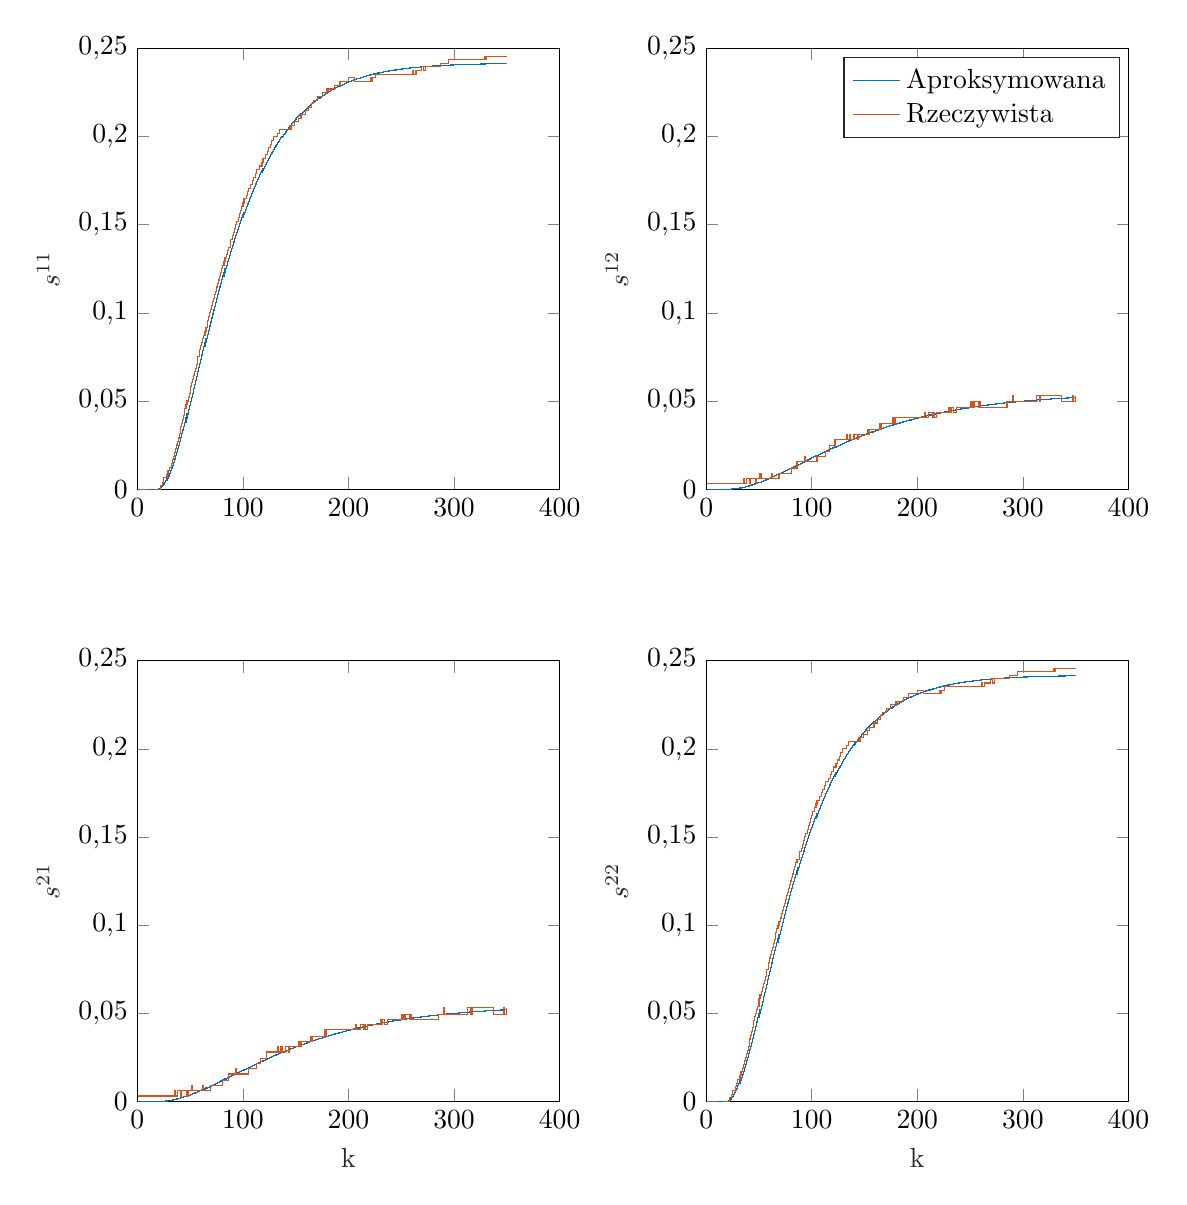
\begin{tikzpicture}

\begin{axis}[%
width=2.111in,
height=2.203in,
at={(0.889in,3.771in)},
scale only axis,
xmin=0,
xmax=400,
xtick={0,100,200,300,400},
ymin=0,
ymax=0.25,
ytick={0,0.05,0.1,0.15,0.2,0.25},
yticklabels={{0},{0,05},{0,1},{0,15},{0,2},{0,25}},
ylabel style={font=\color{white!15!black}},
ylabel={$\text{s}^{\text{11}}$},
axis background/.style={fill=white}
]
\addplot[const plot, color=mycolor1, forget plot] table[row sep=crcr] {%
1	0\\
2	0\\
3	0\\
4	0\\
5	0\\
6	0\\
7	0\\
8	0\\
9	0\\
10	0\\
11	0\\
12	0\\
13	0\\
14	0\\
15	0\\
16	0\\
17	0\\
18	0\\
19	0\\
20	8.7208e-05\\
21	0.0003426\\
22	0.00075709\\
23	0.001322\\
24	0.0020289\\
25	0.0028699\\
26	0.0038372\\
27	0.0049235\\
28	0.0061217\\
29	0.0074251\\
30	0.0088271\\
31	0.010322\\
32	0.011902\\
33	0.013564\\
34	0.015301\\
35	0.017108\\
36	0.01898\\
37	0.020913\\
38	0.022901\\
39	0.024941\\
40	0.027028\\
41	0.029158\\
42	0.031327\\
43	0.033533\\
44	0.03577\\
45	0.038037\\
46	0.040329\\
47	0.042644\\
48	0.04498\\
49	0.047332\\
50	0.049699\\
51	0.052079\\
52	0.054468\\
53	0.056865\\
54	0.059267\\
55	0.061673\\
56	0.06408\\
57	0.066487\\
58	0.068893\\
59	0.071294\\
60	0.073691\\
61	0.076081\\
62	0.078463\\
63	0.080837\\
64	0.083199\\
65	0.08555\\
66	0.087889\\
67	0.090214\\
68	0.092524\\
69	0.094819\\
70	0.097098\\
71	0.09936\\
72	0.1016\\
73	0.10383\\
74	0.10604\\
75	0.10822\\
76	0.11039\\
77	0.11254\\
78	0.11466\\
79	0.11676\\
80	0.11885\\
81	0.12091\\
82	0.12294\\
83	0.12496\\
84	0.12695\\
85	0.12892\\
86	0.13086\\
87	0.13278\\
88	0.13468\\
89	0.13656\\
90	0.13841\\
91	0.14023\\
92	0.14204\\
93	0.14381\\
94	0.14557\\
95	0.1473\\
96	0.14901\\
97	0.15069\\
98	0.15235\\
99	0.15398\\
100	0.15559\\
101	0.15718\\
102	0.15875\\
103	0.16029\\
104	0.1618\\
105	0.1633\\
106	0.16477\\
107	0.16622\\
108	0.16765\\
109	0.16905\\
110	0.17043\\
111	0.17179\\
112	0.17313\\
113	0.17445\\
114	0.17574\\
115	0.17701\\
116	0.17827\\
117	0.1795\\
118	0.18071\\
119	0.1819\\
120	0.18307\\
121	0.18422\\
122	0.18535\\
123	0.18646\\
124	0.18756\\
125	0.18863\\
126	0.18969\\
127	0.19072\\
128	0.19174\\
129	0.19274\\
130	0.19372\\
131	0.19469\\
132	0.19563\\
133	0.19656\\
134	0.19748\\
135	0.19837\\
136	0.19925\\
137	0.20012\\
138	0.20096\\
139	0.2018\\
140	0.20261\\
141	0.20342\\
142	0.2042\\
143	0.20498\\
144	0.20573\\
145	0.20648\\
146	0.20721\\
147	0.20792\\
148	0.20862\\
149	0.20931\\
150	0.20999\\
151	0.21065\\
152	0.2113\\
153	0.21193\\
154	0.21256\\
155	0.21317\\
156	0.21377\\
157	0.21436\\
158	0.21494\\
159	0.2155\\
160	0.21606\\
161	0.2166\\
162	0.21714\\
163	0.21766\\
164	0.21817\\
165	0.21867\\
166	0.21916\\
167	0.21965\\
168	0.22012\\
169	0.22058\\
170	0.22104\\
171	0.22148\\
172	0.22192\\
173	0.22234\\
174	0.22276\\
175	0.22317\\
176	0.22357\\
177	0.22396\\
178	0.22435\\
179	0.22472\\
180	0.22509\\
181	0.22546\\
182	0.22581\\
183	0.22616\\
184	0.2265\\
185	0.22683\\
186	0.22715\\
187	0.22747\\
188	0.22779\\
189	0.22809\\
190	0.22839\\
191	0.22868\\
192	0.22897\\
193	0.22925\\
194	0.22953\\
195	0.2298\\
196	0.23006\\
197	0.23032\\
198	0.23057\\
199	0.23082\\
200	0.23106\\
201	0.2313\\
202	0.23153\\
203	0.23175\\
204	0.23198\\
205	0.23219\\
206	0.23241\\
207	0.23261\\
208	0.23282\\
209	0.23302\\
210	0.23321\\
211	0.2334\\
212	0.23359\\
213	0.23377\\
214	0.23395\\
215	0.23413\\
216	0.2343\\
217	0.23446\\
218	0.23463\\
219	0.23479\\
220	0.23494\\
221	0.2351\\
222	0.23525\\
223	0.23539\\
224	0.23554\\
225	0.23568\\
226	0.23582\\
227	0.23595\\
228	0.23608\\
229	0.23621\\
230	0.23633\\
231	0.23646\\
232	0.23658\\
233	0.2367\\
234	0.23681\\
235	0.23692\\
236	0.23703\\
237	0.23714\\
238	0.23724\\
239	0.23735\\
240	0.23745\\
241	0.23755\\
242	0.23764\\
243	0.23774\\
244	0.23783\\
245	0.23792\\
246	0.23801\\
247	0.23809\\
248	0.23818\\
249	0.23826\\
250	0.23834\\
251	0.23842\\
252	0.23849\\
253	0.23857\\
254	0.23864\\
255	0.23871\\
256	0.23878\\
257	0.23885\\
258	0.23892\\
259	0.23898\\
260	0.23905\\
261	0.23911\\
262	0.23917\\
263	0.23923\\
264	0.23929\\
265	0.23935\\
266	0.2394\\
267	0.23946\\
268	0.23951\\
269	0.23956\\
270	0.23961\\
271	0.23966\\
272	0.23971\\
273	0.23976\\
274	0.2398\\
275	0.23985\\
276	0.23989\\
277	0.23994\\
278	0.23998\\
279	0.24002\\
280	0.24006\\
281	0.2401\\
282	0.24014\\
283	0.24018\\
284	0.24021\\
285	0.24025\\
286	0.24029\\
287	0.24032\\
288	0.24035\\
289	0.24039\\
290	0.24042\\
291	0.24045\\
292	0.24048\\
293	0.24051\\
294	0.24054\\
295	0.24057\\
296	0.2406\\
297	0.24062\\
298	0.24065\\
299	0.24068\\
300	0.2407\\
301	0.24073\\
302	0.24075\\
303	0.24077\\
304	0.2408\\
305	0.24082\\
306	0.24084\\
307	0.24086\\
308	0.24088\\
309	0.2409\\
310	0.24092\\
311	0.24094\\
312	0.24096\\
313	0.24098\\
314	0.241\\
315	0.24102\\
316	0.24104\\
317	0.24105\\
318	0.24107\\
319	0.24109\\
320	0.2411\\
321	0.24112\\
322	0.24113\\
323	0.24115\\
324	0.24116\\
325	0.24118\\
326	0.24119\\
327	0.2412\\
328	0.24122\\
329	0.24123\\
330	0.24124\\
331	0.24125\\
332	0.24127\\
333	0.24128\\
334	0.24129\\
335	0.2413\\
336	0.24131\\
337	0.24132\\
338	0.24133\\
339	0.24134\\
340	0.24135\\
341	0.24136\\
342	0.24137\\
343	0.24138\\
344	0.24139\\
345	0.2414\\
346	0.24141\\
347	0.24142\\
348	0.24142\\
349	0.24143\\
350	0.24144\\
};
\addplot[const plot, color=mycolor2, forget plot] table[row sep=crcr] {%
1	0\\
2	0\\
3	0\\
4	0\\
5	0\\
6	0\\
7	0\\
8	0\\
9	-0.00200000000000008\\
10	-0.00200000000000008\\
11	-0.00200000000000008\\
12	-0.00200000000000008\\
13	-0.00200000000000008\\
14	-0.00200000000000008\\
15	-0.00200000000000008\\
16	-0.00200000000000008\\
17	0\\
18	0\\
19	0\\
20	0\\
21	0\\
22	0.00199999999999984\\
23	0.00199999999999984\\
24	0.00399999999999992\\
25	0.00633333333333326\\
26	0.00633333333333326\\
27	0.00633333333333326\\
28	0.00833333333333333\\
29	0.0103333333333332\\
30	0.0123333333333332\\
31	0.0123333333333332\\
32	0.0146666666666666\\
33	0.0166666666666667\\
34	0.0186666666666665\\
35	0.0206666666666666\\
36	0.0229999999999999\\
37	0.025\\
38	0.0269999999999998\\
39	0.0289999999999999\\
40	0.0313333333333333\\
41	0.0353333333333332\\
42	0.0373333333333332\\
43	0.0396666666666666\\
44	0.0416666666666667\\
45	0.0456666666666666\\
46	0.0479999999999999\\
47	0.05\\
48	0.0519999999999998\\
49	0.0539999999999999\\
50	0.0583333333333333\\
51	0.0603333333333332\\
52	0.0623333333333332\\
53	0.0646666666666666\\
54	0.0666666666666667\\
55	0.0686666666666665\\
56	0.0706666666666666\\
57	0.075\\
58	0.075\\
59	0.0789999999999999\\
60	0.0813333333333333\\
61	0.0833333333333333\\
62	0.0853333333333332\\
63	0.0873333333333332\\
64	0.0896666666666666\\
65	0.0916666666666667\\
66	0.0956666666666666\\
67	0.0979999999999999\\
68	0.1\\
69	0.102\\
70	0.104\\
71	0.106333333333333\\
72	0.108333333333333\\
73	0.110333333333333\\
74	0.112333333333333\\
75	0.114666666666667\\
76	0.116666666666667\\
77	0.118666666666667\\
78	0.120666666666667\\
79	0.123\\
80	0.125\\
81	0.127\\
82	0.129\\
83	0.131333333333333\\
84	0.133333333333333\\
85	0.135333333333333\\
86	0.137333333333333\\
87	0.137333333333333\\
88	0.141666666666667\\
89	0.141666666666667\\
90	0.143666666666667\\
91	0.145666666666667\\
92	0.148\\
93	0.15\\
94	0.152\\
95	0.152\\
96	0.154\\
97	0.156333333333333\\
98	0.158333333333333\\
99	0.160333333333333\\
100	0.162333333333333\\
101	0.164666666666667\\
102	0.164666666666667\\
103	0.166666666666667\\
104	0.168666666666666\\
105	0.170666666666667\\
106	0.170666666666667\\
107	0.173\\
108	0.173\\
109	0.175\\
110	0.177\\
111	0.177\\
112	0.179\\
113	0.181333333333333\\
114	0.181333333333333\\
115	0.181333333333333\\
116	0.183333333333333\\
117	0.183333333333333\\
118	0.185333333333333\\
119	0.187333333333333\\
120	0.187333333333333\\
121	0.189666666666667\\
122	0.189666666666667\\
123	0.191666666666667\\
124	0.193666666666667\\
125	0.193666666666667\\
126	0.195666666666667\\
127	0.198\\
128	0.198\\
129	0.2\\
130	0.2\\
131	0.2\\
132	0.2\\
133	0.202\\
134	0.202\\
135	0.204\\
136	0.204\\
137	0.204\\
138	0.204\\
139	0.204\\
140	0.204\\
141	0.204\\
142	0.204\\
143	0.204\\
144	0.206333333333333\\
145	0.204\\
146	0.206333333333333\\
147	0.206333333333333\\
148	0.206333333333333\\
149	0.208333333333333\\
150	0.208333333333333\\
151	0.208333333333333\\
152	0.208333333333333\\
153	0.210333333333333\\
154	0.210333333333333\\
155	0.212333333333333\\
156	0.212333333333333\\
157	0.212333333333333\\
158	0.212333333333333\\
159	0.214666666666667\\
160	0.214666666666667\\
161	0.214666666666667\\
162	0.216666666666667\\
163	0.216666666666667\\
164	0.216666666666667\\
165	0.218666666666667\\
166	0.218666666666667\\
167	0.220666666666667\\
168	0.220666666666667\\
169	0.220666666666667\\
170	0.220666666666667\\
171	0.223\\
172	0.223\\
173	0.223\\
174	0.223\\
175	0.225\\
176	0.225\\
177	0.225\\
178	0.225\\
179	0.227\\
180	0.225\\
181	0.227\\
182	0.227\\
183	0.227\\
184	0.227\\
185	0.227\\
186	0.227\\
187	0.229\\
188	0.229\\
189	0.229\\
190	0.229\\
191	0.229\\
192	0.231333333333333\\
193	0.231333333333333\\
194	0.231333333333333\\
195	0.231333333333333\\
196	0.231333333333333\\
197	0.231333333333333\\
198	0.231333333333333\\
199	0.231333333333333\\
200	0.233333333333333\\
201	0.233333333333333\\
202	0.233333333333333\\
203	0.233333333333333\\
204	0.233333333333333\\
205	0.233333333333333\\
206	0.231333333333333\\
207	0.231333333333333\\
208	0.231333333333333\\
209	0.231333333333333\\
210	0.231333333333333\\
211	0.231333333333333\\
212	0.231333333333333\\
213	0.231333333333333\\
214	0.231333333333333\\
215	0.231333333333333\\
216	0.231333333333333\\
217	0.231333333333333\\
218	0.231333333333333\\
219	0.231333333333333\\
220	0.231333333333333\\
221	0.233333333333333\\
222	0.231333333333333\\
223	0.233333333333333\\
224	0.233333333333333\\
225	0.233333333333333\\
226	0.235333333333333\\
227	0.235333333333333\\
228	0.235333333333333\\
229	0.235333333333333\\
230	0.235333333333333\\
231	0.235333333333333\\
232	0.235333333333333\\
233	0.235333333333333\\
234	0.235333333333333\\
235	0.235333333333333\\
236	0.235333333333333\\
237	0.235333333333333\\
238	0.235333333333333\\
239	0.235333333333333\\
240	0.235333333333333\\
241	0.235333333333333\\
242	0.235333333333333\\
243	0.235333333333333\\
244	0.235333333333333\\
245	0.235333333333333\\
246	0.235333333333333\\
247	0.235333333333333\\
248	0.235333333333333\\
249	0.235333333333333\\
250	0.235333333333333\\
251	0.235333333333333\\
252	0.235333333333333\\
253	0.235333333333333\\
254	0.235333333333333\\
255	0.235333333333333\\
256	0.235333333333333\\
257	0.235333333333333\\
258	0.235333333333333\\
259	0.235333333333333\\
260	0.235333333333333\\
261	0.237333333333333\\
262	0.235333333333333\\
263	0.235333333333333\\
264	0.237333333333333\\
265	0.237333333333333\\
266	0.237333333333333\\
267	0.237333333333333\\
268	0.237333333333333\\
269	0.239666666666667\\
270	0.239666666666667\\
271	0.237333333333333\\
272	0.237333333333333\\
273	0.239666666666667\\
274	0.239666666666667\\
275	0.239666666666667\\
276	0.239666666666667\\
277	0.239666666666667\\
278	0.239666666666667\\
279	0.239666666666667\\
280	0.239666666666667\\
281	0.239666666666667\\
282	0.239666666666667\\
283	0.239666666666667\\
284	0.239666666666667\\
285	0.239666666666667\\
286	0.239666666666667\\
287	0.241666666666667\\
288	0.241666666666667\\
289	0.241666666666667\\
290	0.241666666666667\\
291	0.241666666666667\\
292	0.241666666666667\\
293	0.241666666666667\\
294	0.241666666666667\\
295	0.243666666666667\\
296	0.243666666666667\\
297	0.243666666666667\\
298	0.243666666666667\\
299	0.243666666666667\\
300	0.243666666666667\\
301	0.243666666666667\\
302	0.243666666666667\\
303	0.243666666666667\\
304	0.243666666666667\\
305	0.243666666666667\\
306	0.243666666666667\\
307	0.243666666666667\\
308	0.243666666666667\\
309	0.243666666666667\\
310	0.243666666666667\\
311	0.243666666666667\\
312	0.243666666666667\\
313	0.243666666666667\\
314	0.243666666666667\\
315	0.243666666666667\\
316	0.243666666666667\\
317	0.243666666666667\\
318	0.243666666666667\\
319	0.243666666666667\\
320	0.243666666666667\\
321	0.243666666666667\\
322	0.243666666666667\\
323	0.243666666666667\\
324	0.243666666666667\\
325	0.243666666666667\\
326	0.243666666666667\\
327	0.243666666666667\\
328	0.243666666666667\\
329	0.245666666666667\\
330	0.243666666666667\\
331	0.245666666666667\\
332	0.245666666666667\\
333	0.245666666666667\\
334	0.245666666666667\\
335	0.245666666666667\\
336	0.245666666666667\\
337	0.245666666666667\\
338	0.245666666666667\\
339	0.245666666666667\\
340	0.245666666666667\\
341	0.245666666666667\\
342	0.245666666666667\\
343	0.245666666666667\\
344	0.245666666666667\\
345	0.245666666666667\\
346	0.245666666666667\\
347	0.245666666666667\\
348	0.245666666666667\\
349	0.245666666666667\\
350	0.245666666666667\\
};
\end{axis}

\begin{axis}[%
width=2.111in,
height=2.203in,
at={(3.733in,3.771in)},
scale only axis,
xmin=0,
xmax=400,
xtick={0,100,200,300,400},
ymin=0,
ymax=0.25,
ytick={0,0.05,0.1,0.15,0.2,0.25},
yticklabels={{0},{0,05},{0,1},{0,15},{0,2},{0,25}},
ylabel style={font=\color{white!15!black}},
ylabel={$\text{s}^{\text{12}}$},
axis background/.style={fill=white},
legend style={legend cell align=left, align=left, draw=white!15!black}
]
\addplot[const plot, color=mycolor1] table[row sep=crcr] {%
1	0\\
2	0\\
3	0\\
4	0\\
5	0\\
6	0\\
7	0\\
8	0\\
9	0\\
10	0\\
11	0\\
12	0\\
13	0\\
14	0\\
15	0\\
16	0\\
17	0\\
18	0\\
19	0\\
20	0\\
21	0\\
22	5.8658e-06\\
23	2.3234e-05\\
24	5.1766e-05\\
25	9.1132e-05\\
26	0.00014101\\
27	0.00020108\\
28	0.00027103\\
29	0.00035056\\
30	0.00043938\\
31	0.0005372\\
32	0.00064373\\
33	0.0007587\\
34	0.00088184\\
35	0.0010129\\
36	0.0011516\\
37	0.0012977\\
38	0.0014509\\
39	0.001611\\
40	0.0017778\\
41	0.0019511\\
42	0.0021305\\
43	0.002316\\
44	0.0025073\\
45	0.0027041\\
46	0.0029063\\
47	0.0031136\\
48	0.003326\\
49	0.0035431\\
50	0.0037648\\
51	0.003991\\
52	0.0042214\\
53	0.0044558\\
54	0.0046942\\
55	0.0049363\\
56	0.005182\\
57	0.005431\\
58	0.0056834\\
59	0.0059389\\
60	0.0061973\\
61	0.0064586\\
62	0.0067225\\
63	0.0069891\\
64	0.007258\\
65	0.0075293\\
66	0.0078027\\
67	0.0080781\\
68	0.0083555\\
69	0.0086347\\
70	0.0089157\\
71	0.0091982\\
72	0.0094822\\
73	0.0097675\\
74	0.010054\\
75	0.010342\\
76	0.010631\\
77	0.010921\\
78	0.011212\\
79	0.011503\\
80	0.011796\\
81	0.012089\\
82	0.012382\\
83	0.012676\\
84	0.012971\\
85	0.013266\\
86	0.013561\\
87	0.013856\\
88	0.014151\\
89	0.014447\\
90	0.014742\\
91	0.015037\\
92	0.015332\\
93	0.015627\\
94	0.015922\\
95	0.016217\\
96	0.016511\\
97	0.016804\\
98	0.017097\\
99	0.01739\\
100	0.017682\\
101	0.017974\\
102	0.018264\\
103	0.018555\\
104	0.018844\\
105	0.019133\\
106	0.01942\\
107	0.019707\\
108	0.019993\\
109	0.020278\\
110	0.020563\\
111	0.020846\\
112	0.021128\\
113	0.021409\\
114	0.021689\\
115	0.021968\\
116	0.022245\\
117	0.022522\\
118	0.022797\\
119	0.023071\\
120	0.023344\\
121	0.023616\\
122	0.023886\\
123	0.024155\\
124	0.024423\\
125	0.024689\\
126	0.024954\\
127	0.025218\\
128	0.02548\\
129	0.025741\\
130	0.026\\
131	0.026258\\
132	0.026514\\
133	0.026769\\
134	0.027023\\
135	0.027275\\
136	0.027526\\
137	0.027775\\
138	0.028022\\
139	0.028268\\
140	0.028512\\
141	0.028755\\
142	0.028997\\
143	0.029236\\
144	0.029475\\
145	0.029711\\
146	0.029946\\
147	0.03018\\
148	0.030412\\
149	0.030642\\
150	0.030871\\
151	0.031098\\
152	0.031323\\
153	0.031547\\
154	0.03177\\
155	0.03199\\
156	0.032209\\
157	0.032427\\
158	0.032643\\
159	0.032857\\
160	0.03307\\
161	0.033281\\
162	0.03349\\
163	0.033698\\
164	0.033905\\
165	0.034109\\
166	0.034313\\
167	0.034514\\
168	0.034714\\
169	0.034912\\
170	0.035109\\
171	0.035304\\
172	0.035498\\
173	0.03569\\
174	0.035881\\
175	0.03607\\
176	0.036257\\
177	0.036443\\
178	0.036627\\
179	0.03681\\
180	0.036991\\
181	0.037171\\
182	0.037349\\
183	0.037526\\
184	0.037701\\
185	0.037875\\
186	0.038047\\
187	0.038218\\
188	0.038387\\
189	0.038555\\
190	0.038721\\
191	0.038886\\
192	0.039049\\
193	0.039211\\
194	0.039372\\
195	0.039531\\
196	0.039688\\
197	0.039844\\
198	0.039999\\
199	0.040153\\
200	0.040305\\
201	0.040455\\
202	0.040604\\
203	0.040752\\
204	0.040899\\
205	0.041044\\
206	0.041188\\
207	0.04133\\
208	0.041471\\
209	0.041611\\
210	0.04175\\
211	0.041887\\
212	0.042023\\
213	0.042158\\
214	0.042291\\
215	0.042423\\
216	0.042554\\
217	0.042683\\
218	0.042812\\
219	0.042939\\
220	0.043065\\
221	0.043189\\
222	0.043313\\
223	0.043435\\
224	0.043556\\
225	0.043676\\
226	0.043795\\
227	0.043912\\
228	0.044029\\
229	0.044144\\
230	0.044258\\
231	0.044371\\
232	0.044483\\
233	0.044593\\
234	0.044703\\
235	0.044812\\
236	0.044919\\
237	0.045025\\
238	0.045131\\
239	0.045235\\
240	0.045338\\
241	0.04544\\
242	0.045541\\
243	0.045641\\
244	0.04574\\
245	0.045838\\
246	0.045935\\
247	0.046032\\
248	0.046127\\
249	0.046221\\
250	0.046314\\
251	0.046406\\
252	0.046497\\
253	0.046587\\
254	0.046677\\
255	0.046765\\
256	0.046853\\
257	0.046939\\
258	0.047025\\
259	0.04711\\
260	0.047193\\
261	0.047276\\
262	0.047358\\
263	0.04744\\
264	0.04752\\
265	0.0476\\
266	0.047678\\
267	0.047756\\
268	0.047833\\
269	0.04791\\
270	0.047985\\
271	0.04806\\
272	0.048133\\
273	0.048206\\
274	0.048279\\
275	0.04835\\
276	0.048421\\
277	0.048491\\
278	0.04856\\
279	0.048628\\
280	0.048696\\
281	0.048763\\
282	0.048829\\
283	0.048895\\
284	0.04896\\
285	0.049024\\
286	0.049087\\
287	0.04915\\
288	0.049212\\
289	0.049273\\
290	0.049334\\
291	0.049394\\
292	0.049453\\
293	0.049512\\
294	0.04957\\
295	0.049627\\
296	0.049684\\
297	0.04974\\
298	0.049796\\
299	0.049851\\
300	0.049905\\
301	0.049959\\
302	0.050012\\
303	0.050064\\
304	0.050116\\
305	0.050168\\
306	0.050219\\
307	0.050269\\
308	0.050318\\
309	0.050368\\
310	0.050416\\
311	0.050464\\
312	0.050512\\
313	0.050559\\
314	0.050605\\
315	0.050651\\
316	0.050696\\
317	0.050741\\
318	0.050786\\
319	0.050829\\
320	0.050873\\
321	0.050916\\
322	0.050958\\
323	0.051\\
324	0.051041\\
325	0.051082\\
326	0.051123\\
327	0.051163\\
328	0.051202\\
329	0.051241\\
330	0.05128\\
331	0.051318\\
332	0.051356\\
333	0.051394\\
334	0.05143\\
335	0.051467\\
336	0.051503\\
337	0.051539\\
338	0.051574\\
339	0.051609\\
340	0.051643\\
341	0.051677\\
342	0.051711\\
343	0.051744\\
344	0.051777\\
345	0.05181\\
346	0.051842\\
347	0.051874\\
348	0.051905\\
349	0.051936\\
350	0.051967\\
};
\addlegendentry{Aproksymowana}

\addplot[const plot, color=mycolor2] table[row sep=crcr] {%
1	0.00300000000000011\\
2	0.00300000000000011\\
3	0.00300000000000011\\
4	0.00300000000000011\\
5	0.00300000000000011\\
6	0.00300000000000011\\
7	0.00300000000000011\\
8	0.00300000000000011\\
9	0.00300000000000011\\
10	0.00300000000000011\\
11	0.00300000000000011\\
12	0.00300000000000011\\
13	0.00300000000000011\\
14	0.00300000000000011\\
15	0.00300000000000011\\
16	0.00300000000000011\\
17	0.00300000000000011\\
18	0.00300000000000011\\
19	0.00300000000000011\\
20	0.00300000000000011\\
21	0.00300000000000011\\
22	0.00300000000000011\\
23	0.00300000000000011\\
24	0.00300000000000011\\
25	0.00300000000000011\\
26	0.00300000000000011\\
27	0.00300000000000011\\
28	0.00300000000000011\\
29	0.00300000000000011\\
30	0.00300000000000011\\
31	0.00300000000000011\\
32	0.00300000000000011\\
33	0.00300000000000011\\
34	0.00300000000000011\\
35	0.00600000000000023\\
36	0.00300000000000011\\
37	0.00300000000000011\\
38	0.00600000000000023\\
39	0.00600000000000023\\
40	0.00600000000000023\\
41	0.00300000000000011\\
42	0.00600000000000023\\
43	0.00600000000000023\\
44	0.00600000000000023\\
45	0.00600000000000023\\
46	0.00600000000000023\\
47	0.00300000000000011\\
48	0.00600000000000023\\
49	0.00600000000000023\\
50	0.00600000000000023\\
51	0.00899999999999999\\
52	0.00600000000000023\\
53	0.00600000000000023\\
54	0.00600000000000023\\
55	0.00600000000000023\\
56	0.00600000000000023\\
57	0.00600000000000023\\
58	0.00600000000000023\\
59	0.00600000000000023\\
60	0.00600000000000023\\
61	0.00600000000000023\\
62	0.00899999999999999\\
63	0.00600000000000023\\
64	0.00600000000000023\\
65	0.00600000000000023\\
66	0.00600000000000023\\
67	0.00600000000000023\\
68	0.00600000000000023\\
69	0.00899999999999999\\
70	0.00899999999999999\\
71	0.00899999999999999\\
72	0.00899999999999999\\
73	0.00899999999999999\\
74	0.00899999999999999\\
75	0.00899999999999999\\
76	0.00899999999999999\\
77	0.00899999999999999\\
78	0.00899999999999999\\
79	0.00899999999999999\\
80	0.00899999999999999\\
81	0.0120000000000001\\
82	0.0120000000000001\\
83	0.0120000000000001\\
84	0.0120000000000001\\
85	0.0120000000000001\\
86	0.0155000000000001\\
87	0.0155000000000001\\
88	0.0155000000000001\\
89	0.0155000000000001\\
90	0.0155000000000001\\
91	0.0155000000000001\\
92	0.0155000000000001\\
93	0.0185000000000002\\
94	0.0155000000000001\\
95	0.0155000000000001\\
96	0.0155000000000001\\
97	0.0155000000000001\\
98	0.0155000000000001\\
99	0.0155000000000001\\
100	0.0155000000000001\\
101	0.0155000000000001\\
102	0.0155000000000001\\
103	0.0155000000000001\\
104	0.0155000000000001\\
105	0.0185000000000002\\
106	0.0185000000000002\\
107	0.0185000000000002\\
108	0.0185000000000002\\
109	0.0185000000000002\\
110	0.0185000000000002\\
111	0.0185000000000002\\
112	0.0185000000000002\\
113	0.0215\\
114	0.0215\\
115	0.0215\\
116	0.0215\\
117	0.0245000000000001\\
118	0.0245000000000001\\
119	0.0245000000000001\\
120	0.0245000000000001\\
121	0.0245000000000001\\
122	0.0280000000000001\\
123	0.0280000000000001\\
124	0.0280000000000001\\
125	0.0280000000000001\\
126	0.0280000000000001\\
127	0.0280000000000001\\
128	0.0280000000000001\\
129	0.0280000000000001\\
130	0.0280000000000001\\
131	0.0280000000000001\\
132	0.0280000000000001\\
133	0.0310000000000002\\
134	0.0280000000000001\\
135	0.0280000000000001\\
136	0.0310000000000002\\
137	0.0280000000000001\\
138	0.0280000000000001\\
139	0.0280000000000001\\
140	0.0310000000000002\\
141	0.0310000000000002\\
142	0.0310000000000002\\
143	0.0280000000000001\\
144	0.0310000000000002\\
145	0.0310000000000002\\
146	0.0310000000000002\\
147	0.0310000000000002\\
148	0.0310000000000002\\
149	0.0310000000000002\\
150	0.0310000000000002\\
151	0.0310000000000002\\
152	0.0310000000000002\\
153	0.034\\
154	0.0310000000000002\\
155	0.034\\
156	0.034\\
157	0.034\\
158	0.034\\
159	0.034\\
160	0.034\\
161	0.034\\
162	0.034\\
163	0.034\\
164	0.0370000000000001\\
165	0.034\\
166	0.0370000000000001\\
167	0.0370000000000001\\
168	0.0370000000000001\\
169	0.0370000000000001\\
170	0.0370000000000001\\
171	0.0370000000000001\\
172	0.0370000000000001\\
173	0.0370000000000001\\
174	0.0370000000000001\\
175	0.0370000000000001\\
176	0.0370000000000001\\
177	0.0405000000000001\\
178	0.0370000000000001\\
179	0.0405000000000001\\
180	0.0405000000000001\\
181	0.0405000000000001\\
182	0.0405000000000001\\
183	0.0405000000000001\\
184	0.0405000000000001\\
185	0.0405000000000001\\
186	0.0405000000000001\\
187	0.0405000000000001\\
188	0.0405000000000001\\
189	0.0405000000000001\\
190	0.0405000000000001\\
191	0.0405000000000001\\
192	0.0405000000000001\\
193	0.0405000000000001\\
194	0.0405000000000001\\
195	0.0405000000000001\\
196	0.0405000000000001\\
197	0.0405000000000001\\
198	0.0405000000000001\\
199	0.0405000000000001\\
200	0.0405000000000001\\
201	0.0405000000000001\\
202	0.0405000000000001\\
203	0.0405000000000001\\
204	0.0405000000000001\\
205	0.0405000000000001\\
206	0.0405000000000001\\
207	0.0435000000000002\\
208	0.0405000000000001\\
209	0.0405000000000001\\
210	0.0405000000000001\\
211	0.0435000000000002\\
212	0.0435000000000002\\
213	0.0435000000000002\\
214	0.0405000000000001\\
215	0.0435000000000002\\
216	0.0405000000000001\\
217	0.0405000000000001\\
218	0.0435000000000002\\
219	0.0435000000000002\\
220	0.0435000000000002\\
221	0.0435000000000002\\
222	0.0435000000000002\\
223	0.0435000000000002\\
224	0.0435000000000002\\
225	0.0435000000000002\\
226	0.0435000000000002\\
227	0.0435000000000002\\
228	0.0435000000000002\\
229	0.0435000000000002\\
230	0.0465\\
231	0.0435000000000002\\
232	0.0465\\
233	0.0465\\
234	0.0435000000000002\\
235	0.0435000000000002\\
236	0.0435000000000002\\
237	0.0465\\
238	0.0465\\
239	0.0465\\
240	0.0465\\
241	0.0465\\
242	0.0465\\
243	0.0465\\
244	0.0465\\
245	0.0465\\
246	0.0465\\
247	0.0465\\
248	0.0465\\
249	0.0465\\
250	0.0495000000000001\\
251	0.0465\\
252	0.0495000000000001\\
253	0.0465\\
254	0.0495000000000001\\
255	0.0495000000000001\\
256	0.0495000000000001\\
257	0.0495000000000001\\
258	0.0465\\
259	0.0495000000000001\\
260	0.0465\\
261	0.0465\\
262	0.0465\\
263	0.0465\\
264	0.0465\\
265	0.0465\\
266	0.0465\\
267	0.0465\\
268	0.0465\\
269	0.0465\\
270	0.0465\\
271	0.0465\\
272	0.0465\\
273	0.0465\\
274	0.0465\\
275	0.0465\\
276	0.0465\\
277	0.0465\\
278	0.0465\\
279	0.0465\\
280	0.0465\\
281	0.0465\\
282	0.0465\\
283	0.0465\\
284	0.0465\\
285	0.0495000000000001\\
286	0.0495000000000001\\
287	0.0495000000000001\\
288	0.0495000000000001\\
289	0.0495000000000001\\
290	0.0530000000000001\\
291	0.0495000000000001\\
292	0.0495000000000001\\
293	0.0495000000000001\\
294	0.0495000000000001\\
295	0.0495000000000001\\
296	0.0495000000000001\\
297	0.0495000000000001\\
298	0.0495000000000001\\
299	0.0495000000000001\\
300	0.0495000000000001\\
301	0.0495000000000001\\
302	0.0495000000000001\\
303	0.0495000000000001\\
304	0.0495000000000001\\
305	0.0495000000000001\\
306	0.0495000000000001\\
307	0.0495000000000001\\
308	0.0495000000000001\\
309	0.0495000000000001\\
310	0.0495000000000001\\
311	0.0495000000000001\\
312	0.0495000000000001\\
313	0.0530000000000001\\
314	0.0530000000000001\\
315	0.0530000000000001\\
316	0.0495000000000001\\
317	0.0530000000000001\\
318	0.0530000000000001\\
319	0.0530000000000001\\
320	0.0530000000000001\\
321	0.0530000000000001\\
322	0.0530000000000001\\
323	0.0530000000000001\\
324	0.0530000000000001\\
325	0.0530000000000001\\
326	0.0530000000000001\\
327	0.0530000000000001\\
328	0.0530000000000001\\
329	0.0530000000000001\\
330	0.0530000000000001\\
331	0.0530000000000001\\
332	0.0530000000000001\\
333	0.0530000000000001\\
334	0.0530000000000001\\
335	0.0530000000000001\\
336	0.0530000000000001\\
337	0.0495000000000001\\
338	0.0495000000000001\\
339	0.0495000000000001\\
340	0.0495000000000001\\
341	0.0495000000000001\\
342	0.0495000000000001\\
343	0.0495000000000001\\
344	0.0495000000000001\\
345	0.0495000000000001\\
346	0.0495000000000001\\
347	0.0530000000000001\\
348	0.0495000000000001\\
349	0.0495000000000001\\
350	0.0530000000000001\\
};
\addlegendentry{Rzeczywista}

\end{axis}

\begin{axis}[%
width=2.111in,
height=2.203in,
at={(0.889in,0.71in)},
scale only axis,
xmin=0,
xmax=400,
xtick={0,100,200,300,400},
xlabel style={font=\color{white!15!black}},
xlabel={k},
ymin=0,
ymax=0.25,
ytick={0,0.05,0.1,0.15,0.2,0.25},
yticklabels={{0},{0,05},{0,1},{0,15},{0,2},{0,25}},
ylabel style={font=\color{white!15!black}},
ylabel={$\text{s}^{\text{21}}$},
axis background/.style={fill=white}
]
\addplot[const plot, color=mycolor1, forget plot] table[row sep=crcr] {%
1	0\\
2	0\\
3	0\\
4	0\\
5	0\\
6	0\\
7	0\\
8	0\\
9	0\\
10	0\\
11	0\\
12	0\\
13	0\\
14	0\\
15	0\\
16	0\\
17	0\\
18	0\\
19	0\\
20	0\\
21	0\\
22	5.8658e-06\\
23	2.3234e-05\\
24	5.1766e-05\\
25	9.1132e-05\\
26	0.00014101\\
27	0.00020108\\
28	0.00027103\\
29	0.00035056\\
30	0.00043938\\
31	0.0005372\\
32	0.00064373\\
33	0.0007587\\
34	0.00088184\\
35	0.0010129\\
36	0.0011516\\
37	0.0012977\\
38	0.0014509\\
39	0.001611\\
40	0.0017778\\
41	0.0019511\\
42	0.0021305\\
43	0.002316\\
44	0.0025073\\
45	0.0027041\\
46	0.0029063\\
47	0.0031136\\
48	0.003326\\
49	0.0035431\\
50	0.0037648\\
51	0.003991\\
52	0.0042214\\
53	0.0044558\\
54	0.0046942\\
55	0.0049363\\
56	0.005182\\
57	0.005431\\
58	0.0056834\\
59	0.0059389\\
60	0.0061973\\
61	0.0064586\\
62	0.0067225\\
63	0.0069891\\
64	0.007258\\
65	0.0075293\\
66	0.0078027\\
67	0.0080781\\
68	0.0083555\\
69	0.0086347\\
70	0.0089157\\
71	0.0091982\\
72	0.0094822\\
73	0.0097675\\
74	0.010054\\
75	0.010342\\
76	0.010631\\
77	0.010921\\
78	0.011212\\
79	0.011503\\
80	0.011796\\
81	0.012089\\
82	0.012382\\
83	0.012676\\
84	0.012971\\
85	0.013266\\
86	0.013561\\
87	0.013856\\
88	0.014151\\
89	0.014447\\
90	0.014742\\
91	0.015037\\
92	0.015332\\
93	0.015627\\
94	0.015922\\
95	0.016217\\
96	0.016511\\
97	0.016804\\
98	0.017097\\
99	0.01739\\
100	0.017682\\
101	0.017974\\
102	0.018264\\
103	0.018555\\
104	0.018844\\
105	0.019133\\
106	0.01942\\
107	0.019707\\
108	0.019993\\
109	0.020278\\
110	0.020563\\
111	0.020846\\
112	0.021128\\
113	0.021409\\
114	0.021689\\
115	0.021968\\
116	0.022245\\
117	0.022522\\
118	0.022797\\
119	0.023071\\
120	0.023344\\
121	0.023616\\
122	0.023886\\
123	0.024155\\
124	0.024423\\
125	0.024689\\
126	0.024954\\
127	0.025218\\
128	0.02548\\
129	0.025741\\
130	0.026\\
131	0.026258\\
132	0.026514\\
133	0.026769\\
134	0.027023\\
135	0.027275\\
136	0.027526\\
137	0.027775\\
138	0.028022\\
139	0.028268\\
140	0.028512\\
141	0.028755\\
142	0.028997\\
143	0.029236\\
144	0.029475\\
145	0.029711\\
146	0.029946\\
147	0.03018\\
148	0.030412\\
149	0.030642\\
150	0.030871\\
151	0.031098\\
152	0.031323\\
153	0.031547\\
154	0.03177\\
155	0.03199\\
156	0.032209\\
157	0.032427\\
158	0.032643\\
159	0.032857\\
160	0.03307\\
161	0.033281\\
162	0.03349\\
163	0.033698\\
164	0.033905\\
165	0.034109\\
166	0.034313\\
167	0.034514\\
168	0.034714\\
169	0.034912\\
170	0.035109\\
171	0.035304\\
172	0.035498\\
173	0.03569\\
174	0.035881\\
175	0.03607\\
176	0.036257\\
177	0.036443\\
178	0.036627\\
179	0.03681\\
180	0.036991\\
181	0.037171\\
182	0.037349\\
183	0.037526\\
184	0.037701\\
185	0.037875\\
186	0.038047\\
187	0.038218\\
188	0.038387\\
189	0.038555\\
190	0.038721\\
191	0.038886\\
192	0.039049\\
193	0.039211\\
194	0.039372\\
195	0.039531\\
196	0.039688\\
197	0.039844\\
198	0.039999\\
199	0.040153\\
200	0.040305\\
201	0.040455\\
202	0.040604\\
203	0.040752\\
204	0.040899\\
205	0.041044\\
206	0.041188\\
207	0.04133\\
208	0.041471\\
209	0.041611\\
210	0.04175\\
211	0.041887\\
212	0.042023\\
213	0.042158\\
214	0.042291\\
215	0.042423\\
216	0.042554\\
217	0.042683\\
218	0.042812\\
219	0.042939\\
220	0.043065\\
221	0.043189\\
222	0.043313\\
223	0.043435\\
224	0.043556\\
225	0.043676\\
226	0.043795\\
227	0.043912\\
228	0.044029\\
229	0.044144\\
230	0.044258\\
231	0.044371\\
232	0.044483\\
233	0.044593\\
234	0.044703\\
235	0.044812\\
236	0.044919\\
237	0.045025\\
238	0.045131\\
239	0.045235\\
240	0.045338\\
241	0.04544\\
242	0.045541\\
243	0.045641\\
244	0.04574\\
245	0.045838\\
246	0.045935\\
247	0.046032\\
248	0.046127\\
249	0.046221\\
250	0.046314\\
251	0.046406\\
252	0.046497\\
253	0.046587\\
254	0.046677\\
255	0.046765\\
256	0.046853\\
257	0.046939\\
258	0.047025\\
259	0.04711\\
260	0.047193\\
261	0.047276\\
262	0.047358\\
263	0.04744\\
264	0.04752\\
265	0.0476\\
266	0.047678\\
267	0.047756\\
268	0.047833\\
269	0.04791\\
270	0.047985\\
271	0.04806\\
272	0.048133\\
273	0.048206\\
274	0.048279\\
275	0.04835\\
276	0.048421\\
277	0.048491\\
278	0.04856\\
279	0.048628\\
280	0.048696\\
281	0.048763\\
282	0.048829\\
283	0.048895\\
284	0.04896\\
285	0.049024\\
286	0.049087\\
287	0.04915\\
288	0.049212\\
289	0.049273\\
290	0.049334\\
291	0.049394\\
292	0.049453\\
293	0.049512\\
294	0.04957\\
295	0.049627\\
296	0.049684\\
297	0.04974\\
298	0.049796\\
299	0.049851\\
300	0.049905\\
301	0.049959\\
302	0.050012\\
303	0.050064\\
304	0.050116\\
305	0.050168\\
306	0.050219\\
307	0.050269\\
308	0.050318\\
309	0.050368\\
310	0.050416\\
311	0.050464\\
312	0.050512\\
313	0.050559\\
314	0.050605\\
315	0.050651\\
316	0.050696\\
317	0.050741\\
318	0.050786\\
319	0.050829\\
320	0.050873\\
321	0.050916\\
322	0.050958\\
323	0.051\\
324	0.051041\\
325	0.051082\\
326	0.051123\\
327	0.051163\\
328	0.051202\\
329	0.051241\\
330	0.05128\\
331	0.051318\\
332	0.051356\\
333	0.051394\\
334	0.05143\\
335	0.051467\\
336	0.051503\\
337	0.051539\\
338	0.051574\\
339	0.051609\\
340	0.051643\\
341	0.051677\\
342	0.051711\\
343	0.051744\\
344	0.051777\\
345	0.05181\\
346	0.051842\\
347	0.051874\\
348	0.051905\\
349	0.051936\\
350	0.051967\\
};
\addplot[const plot, color=mycolor2, forget plot] table[row sep=crcr] {%
1	0.00300000000000011\\
2	0.00300000000000011\\
3	0.00300000000000011\\
4	0.00300000000000011\\
5	0.00300000000000011\\
6	0.00300000000000011\\
7	0.00300000000000011\\
8	0.00300000000000011\\
9	0.00300000000000011\\
10	0.00300000000000011\\
11	0.00300000000000011\\
12	0.00300000000000011\\
13	0.00300000000000011\\
14	0.00300000000000011\\
15	0.00300000000000011\\
16	0.00300000000000011\\
17	0.00300000000000011\\
18	0.00300000000000011\\
19	0.00300000000000011\\
20	0.00300000000000011\\
21	0.00300000000000011\\
22	0.00300000000000011\\
23	0.00300000000000011\\
24	0.00300000000000011\\
25	0.00300000000000011\\
26	0.00300000000000011\\
27	0.00300000000000011\\
28	0.00300000000000011\\
29	0.00300000000000011\\
30	0.00300000000000011\\
31	0.00300000000000011\\
32	0.00300000000000011\\
33	0.00300000000000011\\
34	0.00300000000000011\\
35	0.00600000000000023\\
36	0.00300000000000011\\
37	0.00300000000000011\\
38	0.00600000000000023\\
39	0.00600000000000023\\
40	0.00600000000000023\\
41	0.00300000000000011\\
42	0.00600000000000023\\
43	0.00600000000000023\\
44	0.00600000000000023\\
45	0.00600000000000023\\
46	0.00600000000000023\\
47	0.00300000000000011\\
48	0.00600000000000023\\
49	0.00600000000000023\\
50	0.00600000000000023\\
51	0.00899999999999999\\
52	0.00600000000000023\\
53	0.00600000000000023\\
54	0.00600000000000023\\
55	0.00600000000000023\\
56	0.00600000000000023\\
57	0.00600000000000023\\
58	0.00600000000000023\\
59	0.00600000000000023\\
60	0.00600000000000023\\
61	0.00600000000000023\\
62	0.00899999999999999\\
63	0.00600000000000023\\
64	0.00600000000000023\\
65	0.00600000000000023\\
66	0.00600000000000023\\
67	0.00600000000000023\\
68	0.00600000000000023\\
69	0.00899999999999999\\
70	0.00899999999999999\\
71	0.00899999999999999\\
72	0.00899999999999999\\
73	0.00899999999999999\\
74	0.00899999999999999\\
75	0.00899999999999999\\
76	0.00899999999999999\\
77	0.00899999999999999\\
78	0.00899999999999999\\
79	0.00899999999999999\\
80	0.00899999999999999\\
81	0.0120000000000001\\
82	0.0120000000000001\\
83	0.0120000000000001\\
84	0.0120000000000001\\
85	0.0120000000000001\\
86	0.0155000000000001\\
87	0.0155000000000001\\
88	0.0155000000000001\\
89	0.0155000000000001\\
90	0.0155000000000001\\
91	0.0155000000000001\\
92	0.0155000000000001\\
93	0.0185000000000002\\
94	0.0155000000000001\\
95	0.0155000000000001\\
96	0.0155000000000001\\
97	0.0155000000000001\\
98	0.0155000000000001\\
99	0.0155000000000001\\
100	0.0155000000000001\\
101	0.0155000000000001\\
102	0.0155000000000001\\
103	0.0155000000000001\\
104	0.0155000000000001\\
105	0.0185000000000002\\
106	0.0185000000000002\\
107	0.0185000000000002\\
108	0.0185000000000002\\
109	0.0185000000000002\\
110	0.0185000000000002\\
111	0.0185000000000002\\
112	0.0185000000000002\\
113	0.0215\\
114	0.0215\\
115	0.0215\\
116	0.0215\\
117	0.0245000000000001\\
118	0.0245000000000001\\
119	0.0245000000000001\\
120	0.0245000000000001\\
121	0.0245000000000001\\
122	0.0280000000000001\\
123	0.0280000000000001\\
124	0.0280000000000001\\
125	0.0280000000000001\\
126	0.0280000000000001\\
127	0.0280000000000001\\
128	0.0280000000000001\\
129	0.0280000000000001\\
130	0.0280000000000001\\
131	0.0280000000000001\\
132	0.0280000000000001\\
133	0.0310000000000002\\
134	0.0280000000000001\\
135	0.0280000000000001\\
136	0.0310000000000002\\
137	0.0280000000000001\\
138	0.0280000000000001\\
139	0.0280000000000001\\
140	0.0310000000000002\\
141	0.0310000000000002\\
142	0.0310000000000002\\
143	0.0280000000000001\\
144	0.0310000000000002\\
145	0.0310000000000002\\
146	0.0310000000000002\\
147	0.0310000000000002\\
148	0.0310000000000002\\
149	0.0310000000000002\\
150	0.0310000000000002\\
151	0.0310000000000002\\
152	0.0310000000000002\\
153	0.034\\
154	0.0310000000000002\\
155	0.034\\
156	0.034\\
157	0.034\\
158	0.034\\
159	0.034\\
160	0.034\\
161	0.034\\
162	0.034\\
163	0.034\\
164	0.0370000000000001\\
165	0.034\\
166	0.0370000000000001\\
167	0.0370000000000001\\
168	0.0370000000000001\\
169	0.0370000000000001\\
170	0.0370000000000001\\
171	0.0370000000000001\\
172	0.0370000000000001\\
173	0.0370000000000001\\
174	0.0370000000000001\\
175	0.0370000000000001\\
176	0.0370000000000001\\
177	0.0405000000000001\\
178	0.0370000000000001\\
179	0.0405000000000001\\
180	0.0405000000000001\\
181	0.0405000000000001\\
182	0.0405000000000001\\
183	0.0405000000000001\\
184	0.0405000000000001\\
185	0.0405000000000001\\
186	0.0405000000000001\\
187	0.0405000000000001\\
188	0.0405000000000001\\
189	0.0405000000000001\\
190	0.0405000000000001\\
191	0.0405000000000001\\
192	0.0405000000000001\\
193	0.0405000000000001\\
194	0.0405000000000001\\
195	0.0405000000000001\\
196	0.0405000000000001\\
197	0.0405000000000001\\
198	0.0405000000000001\\
199	0.0405000000000001\\
200	0.0405000000000001\\
201	0.0405000000000001\\
202	0.0405000000000001\\
203	0.0405000000000001\\
204	0.0405000000000001\\
205	0.0405000000000001\\
206	0.0405000000000001\\
207	0.0435000000000002\\
208	0.0405000000000001\\
209	0.0405000000000001\\
210	0.0405000000000001\\
211	0.0435000000000002\\
212	0.0435000000000002\\
213	0.0435000000000002\\
214	0.0405000000000001\\
215	0.0435000000000002\\
216	0.0405000000000001\\
217	0.0405000000000001\\
218	0.0435000000000002\\
219	0.0435000000000002\\
220	0.0435000000000002\\
221	0.0435000000000002\\
222	0.0435000000000002\\
223	0.0435000000000002\\
224	0.0435000000000002\\
225	0.0435000000000002\\
226	0.0435000000000002\\
227	0.0435000000000002\\
228	0.0435000000000002\\
229	0.0435000000000002\\
230	0.0465\\
231	0.0435000000000002\\
232	0.0465\\
233	0.0465\\
234	0.0435000000000002\\
235	0.0435000000000002\\
236	0.0435000000000002\\
237	0.0465\\
238	0.0465\\
239	0.0465\\
240	0.0465\\
241	0.0465\\
242	0.0465\\
243	0.0465\\
244	0.0465\\
245	0.0465\\
246	0.0465\\
247	0.0465\\
248	0.0465\\
249	0.0465\\
250	0.0495000000000001\\
251	0.0465\\
252	0.0495000000000001\\
253	0.0465\\
254	0.0495000000000001\\
255	0.0495000000000001\\
256	0.0495000000000001\\
257	0.0495000000000001\\
258	0.0465\\
259	0.0495000000000001\\
260	0.0465\\
261	0.0465\\
262	0.0465\\
263	0.0465\\
264	0.0465\\
265	0.0465\\
266	0.0465\\
267	0.0465\\
268	0.0465\\
269	0.0465\\
270	0.0465\\
271	0.0465\\
272	0.0465\\
273	0.0465\\
274	0.0465\\
275	0.0465\\
276	0.0465\\
277	0.0465\\
278	0.0465\\
279	0.0465\\
280	0.0465\\
281	0.0465\\
282	0.0465\\
283	0.0465\\
284	0.0465\\
285	0.0495000000000001\\
286	0.0495000000000001\\
287	0.0495000000000001\\
288	0.0495000000000001\\
289	0.0495000000000001\\
290	0.0530000000000001\\
291	0.0495000000000001\\
292	0.0495000000000001\\
293	0.0495000000000001\\
294	0.0495000000000001\\
295	0.0495000000000001\\
296	0.0495000000000001\\
297	0.0495000000000001\\
298	0.0495000000000001\\
299	0.0495000000000001\\
300	0.0495000000000001\\
301	0.0495000000000001\\
302	0.0495000000000001\\
303	0.0495000000000001\\
304	0.0495000000000001\\
305	0.0495000000000001\\
306	0.0495000000000001\\
307	0.0495000000000001\\
308	0.0495000000000001\\
309	0.0495000000000001\\
310	0.0495000000000001\\
311	0.0495000000000001\\
312	0.0495000000000001\\
313	0.0530000000000001\\
314	0.0530000000000001\\
315	0.0530000000000001\\
316	0.0495000000000001\\
317	0.0530000000000001\\
318	0.0530000000000001\\
319	0.0530000000000001\\
320	0.0530000000000001\\
321	0.0530000000000001\\
322	0.0530000000000001\\
323	0.0530000000000001\\
324	0.0530000000000001\\
325	0.0530000000000001\\
326	0.0530000000000001\\
327	0.0530000000000001\\
328	0.0530000000000001\\
329	0.0530000000000001\\
330	0.0530000000000001\\
331	0.0530000000000001\\
332	0.0530000000000001\\
333	0.0530000000000001\\
334	0.0530000000000001\\
335	0.0530000000000001\\
336	0.0530000000000001\\
337	0.0495000000000001\\
338	0.0495000000000001\\
339	0.0495000000000001\\
340	0.0495000000000001\\
341	0.0495000000000001\\
342	0.0495000000000001\\
343	0.0495000000000001\\
344	0.0495000000000001\\
345	0.0495000000000001\\
346	0.0495000000000001\\
347	0.0530000000000001\\
348	0.0495000000000001\\
349	0.0495000000000001\\
350	0.0530000000000001\\
};
\end{axis}

\begin{axis}[%
width=2.111in,
height=2.203in,
at={(3.733in,0.71in)},
scale only axis,
xmin=0,
xmax=400,
xtick={0,100,200,300,400},
xlabel style={font=\color{white!15!black}},
xlabel={k},
ymin=0,
ymax=0.25,
ytick={0,0.05,0.1,0.15,0.2,0.25},
yticklabels={{0},{0,05},{0,1},{0,15},{0,2},{0,25}},
ylabel style={font=\color{white!15!black}},
ylabel={$\text{s}^{\text{22}}$},
axis background/.style={fill=white}
]
\addplot[const plot, color=mycolor1, forget plot] table[row sep=crcr] {%
1	0\\
2	0\\
3	0\\
4	0\\
5	0\\
6	0\\
7	0\\
8	0\\
9	0\\
10	0\\
11	0\\
12	0\\
13	0\\
14	0\\
15	0\\
16	0\\
17	0\\
18	0\\
19	0\\
20	8.7208e-05\\
21	0.0003426\\
22	0.00075709\\
23	0.001322\\
24	0.0020289\\
25	0.0028699\\
26	0.0038372\\
27	0.0049235\\
28	0.0061217\\
29	0.0074251\\
30	0.0088271\\
31	0.010322\\
32	0.011902\\
33	0.013564\\
34	0.015301\\
35	0.017108\\
36	0.01898\\
37	0.020913\\
38	0.022901\\
39	0.024941\\
40	0.027028\\
41	0.029158\\
42	0.031327\\
43	0.033533\\
44	0.03577\\
45	0.038037\\
46	0.040329\\
47	0.042644\\
48	0.04498\\
49	0.047332\\
50	0.049699\\
51	0.052079\\
52	0.054468\\
53	0.056865\\
54	0.059267\\
55	0.061673\\
56	0.06408\\
57	0.066487\\
58	0.068893\\
59	0.071294\\
60	0.073691\\
61	0.076081\\
62	0.078463\\
63	0.080837\\
64	0.083199\\
65	0.08555\\
66	0.087889\\
67	0.090214\\
68	0.092524\\
69	0.094819\\
70	0.097098\\
71	0.09936\\
72	0.1016\\
73	0.10383\\
74	0.10604\\
75	0.10822\\
76	0.11039\\
77	0.11254\\
78	0.11466\\
79	0.11676\\
80	0.11885\\
81	0.12091\\
82	0.12294\\
83	0.12496\\
84	0.12695\\
85	0.12892\\
86	0.13086\\
87	0.13278\\
88	0.13468\\
89	0.13656\\
90	0.13841\\
91	0.14023\\
92	0.14204\\
93	0.14381\\
94	0.14557\\
95	0.1473\\
96	0.14901\\
97	0.15069\\
98	0.15235\\
99	0.15398\\
100	0.15559\\
101	0.15718\\
102	0.15875\\
103	0.16029\\
104	0.1618\\
105	0.1633\\
106	0.16477\\
107	0.16622\\
108	0.16765\\
109	0.16905\\
110	0.17043\\
111	0.17179\\
112	0.17313\\
113	0.17445\\
114	0.17574\\
115	0.17701\\
116	0.17827\\
117	0.1795\\
118	0.18071\\
119	0.1819\\
120	0.18307\\
121	0.18422\\
122	0.18535\\
123	0.18646\\
124	0.18756\\
125	0.18863\\
126	0.18969\\
127	0.19072\\
128	0.19174\\
129	0.19274\\
130	0.19372\\
131	0.19469\\
132	0.19563\\
133	0.19656\\
134	0.19748\\
135	0.19837\\
136	0.19925\\
137	0.20012\\
138	0.20096\\
139	0.2018\\
140	0.20261\\
141	0.20342\\
142	0.2042\\
143	0.20498\\
144	0.20573\\
145	0.20648\\
146	0.20721\\
147	0.20792\\
148	0.20862\\
149	0.20931\\
150	0.20999\\
151	0.21065\\
152	0.2113\\
153	0.21193\\
154	0.21256\\
155	0.21317\\
156	0.21377\\
157	0.21436\\
158	0.21494\\
159	0.2155\\
160	0.21606\\
161	0.2166\\
162	0.21714\\
163	0.21766\\
164	0.21817\\
165	0.21867\\
166	0.21916\\
167	0.21965\\
168	0.22012\\
169	0.22058\\
170	0.22104\\
171	0.22148\\
172	0.22192\\
173	0.22234\\
174	0.22276\\
175	0.22317\\
176	0.22357\\
177	0.22396\\
178	0.22435\\
179	0.22472\\
180	0.22509\\
181	0.22546\\
182	0.22581\\
183	0.22616\\
184	0.2265\\
185	0.22683\\
186	0.22715\\
187	0.22747\\
188	0.22779\\
189	0.22809\\
190	0.22839\\
191	0.22868\\
192	0.22897\\
193	0.22925\\
194	0.22953\\
195	0.2298\\
196	0.23006\\
197	0.23032\\
198	0.23057\\
199	0.23082\\
200	0.23106\\
201	0.2313\\
202	0.23153\\
203	0.23175\\
204	0.23198\\
205	0.23219\\
206	0.23241\\
207	0.23261\\
208	0.23282\\
209	0.23302\\
210	0.23321\\
211	0.2334\\
212	0.23359\\
213	0.23377\\
214	0.23395\\
215	0.23413\\
216	0.2343\\
217	0.23446\\
218	0.23463\\
219	0.23479\\
220	0.23494\\
221	0.2351\\
222	0.23525\\
223	0.23539\\
224	0.23554\\
225	0.23568\\
226	0.23582\\
227	0.23595\\
228	0.23608\\
229	0.23621\\
230	0.23633\\
231	0.23646\\
232	0.23658\\
233	0.2367\\
234	0.23681\\
235	0.23692\\
236	0.23703\\
237	0.23714\\
238	0.23724\\
239	0.23735\\
240	0.23745\\
241	0.23755\\
242	0.23764\\
243	0.23774\\
244	0.23783\\
245	0.23792\\
246	0.23801\\
247	0.23809\\
248	0.23818\\
249	0.23826\\
250	0.23834\\
251	0.23842\\
252	0.23849\\
253	0.23857\\
254	0.23864\\
255	0.23871\\
256	0.23878\\
257	0.23885\\
258	0.23892\\
259	0.23898\\
260	0.23905\\
261	0.23911\\
262	0.23917\\
263	0.23923\\
264	0.23929\\
265	0.23935\\
266	0.2394\\
267	0.23946\\
268	0.23951\\
269	0.23956\\
270	0.23961\\
271	0.23966\\
272	0.23971\\
273	0.23976\\
274	0.2398\\
275	0.23985\\
276	0.23989\\
277	0.23994\\
278	0.23998\\
279	0.24002\\
280	0.24006\\
281	0.2401\\
282	0.24014\\
283	0.24018\\
284	0.24021\\
285	0.24025\\
286	0.24029\\
287	0.24032\\
288	0.24035\\
289	0.24039\\
290	0.24042\\
291	0.24045\\
292	0.24048\\
293	0.24051\\
294	0.24054\\
295	0.24057\\
296	0.2406\\
297	0.24062\\
298	0.24065\\
299	0.24068\\
300	0.2407\\
301	0.24073\\
302	0.24075\\
303	0.24077\\
304	0.2408\\
305	0.24082\\
306	0.24084\\
307	0.24086\\
308	0.24088\\
309	0.2409\\
310	0.24092\\
311	0.24094\\
312	0.24096\\
313	0.24098\\
314	0.241\\
315	0.24102\\
316	0.24104\\
317	0.24105\\
318	0.24107\\
319	0.24109\\
320	0.2411\\
321	0.24112\\
322	0.24113\\
323	0.24115\\
324	0.24116\\
325	0.24118\\
326	0.24119\\
327	0.2412\\
328	0.24122\\
329	0.24123\\
330	0.24124\\
331	0.24125\\
332	0.24127\\
333	0.24128\\
334	0.24129\\
335	0.2413\\
336	0.24131\\
337	0.24132\\
338	0.24133\\
339	0.24134\\
340	0.24135\\
341	0.24136\\
342	0.24137\\
343	0.24138\\
344	0.24139\\
345	0.2414\\
346	0.24141\\
347	0.24142\\
348	0.24142\\
349	0.24143\\
350	0.24144\\
};
\addplot[const plot, color=mycolor2, forget plot] table[row sep=crcr] {%
1	0\\
2	0\\
3	0\\
4	0\\
5	0\\
6	0\\
7	0\\
8	0\\
9	-0.00200000000000008\\
10	-0.00200000000000008\\
11	-0.00200000000000008\\
12	-0.00200000000000008\\
13	-0.00200000000000008\\
14	-0.00200000000000008\\
15	-0.00200000000000008\\
16	-0.00200000000000008\\
17	0\\
18	0\\
19	0\\
20	0\\
21	0\\
22	0.00199999999999984\\
23	0.00199999999999984\\
24	0.00399999999999992\\
25	0.00633333333333326\\
26	0.00633333333333326\\
27	0.00633333333333326\\
28	0.00833333333333333\\
29	0.0103333333333332\\
30	0.0123333333333332\\
31	0.0123333333333332\\
32	0.0146666666666666\\
33	0.0166666666666667\\
34	0.0186666666666665\\
35	0.0206666666666666\\
36	0.0229999999999999\\
37	0.025\\
38	0.0269999999999998\\
39	0.0289999999999999\\
40	0.0313333333333333\\
41	0.0353333333333332\\
42	0.0373333333333332\\
43	0.0396666666666666\\
44	0.0416666666666667\\
45	0.0456666666666666\\
46	0.0479999999999999\\
47	0.05\\
48	0.0519999999999998\\
49	0.0539999999999999\\
50	0.0583333333333333\\
51	0.0603333333333332\\
52	0.0623333333333332\\
53	0.0646666666666666\\
54	0.0666666666666667\\
55	0.0686666666666665\\
56	0.0706666666666666\\
57	0.075\\
58	0.075\\
59	0.0789999999999999\\
60	0.0813333333333333\\
61	0.0833333333333333\\
62	0.0853333333333332\\
63	0.0873333333333332\\
64	0.0896666666666666\\
65	0.0916666666666667\\
66	0.0956666666666666\\
67	0.0979999999999999\\
68	0.1\\
69	0.102\\
70	0.104\\
71	0.106333333333333\\
72	0.108333333333333\\
73	0.110333333333333\\
74	0.112333333333333\\
75	0.114666666666667\\
76	0.116666666666667\\
77	0.118666666666667\\
78	0.120666666666667\\
79	0.123\\
80	0.125\\
81	0.127\\
82	0.129\\
83	0.131333333333333\\
84	0.133333333333333\\
85	0.135333333333333\\
86	0.137333333333333\\
87	0.137333333333333\\
88	0.141666666666667\\
89	0.141666666666667\\
90	0.143666666666667\\
91	0.145666666666667\\
92	0.148\\
93	0.15\\
94	0.152\\
95	0.152\\
96	0.154\\
97	0.156333333333333\\
98	0.158333333333333\\
99	0.160333333333333\\
100	0.162333333333333\\
101	0.164666666666667\\
102	0.164666666666667\\
103	0.166666666666667\\
104	0.168666666666666\\
105	0.170666666666667\\
106	0.170666666666667\\
107	0.173\\
108	0.173\\
109	0.175\\
110	0.177\\
111	0.177\\
112	0.179\\
113	0.181333333333333\\
114	0.181333333333333\\
115	0.181333333333333\\
116	0.183333333333333\\
117	0.183333333333333\\
118	0.185333333333333\\
119	0.187333333333333\\
120	0.187333333333333\\
121	0.189666666666667\\
122	0.189666666666667\\
123	0.191666666666667\\
124	0.193666666666667\\
125	0.193666666666667\\
126	0.195666666666667\\
127	0.198\\
128	0.198\\
129	0.2\\
130	0.2\\
131	0.2\\
132	0.2\\
133	0.202\\
134	0.202\\
135	0.204\\
136	0.204\\
137	0.204\\
138	0.204\\
139	0.204\\
140	0.204\\
141	0.204\\
142	0.204\\
143	0.204\\
144	0.206333333333333\\
145	0.204\\
146	0.206333333333333\\
147	0.206333333333333\\
148	0.206333333333333\\
149	0.208333333333333\\
150	0.208333333333333\\
151	0.208333333333333\\
152	0.208333333333333\\
153	0.210333333333333\\
154	0.210333333333333\\
155	0.212333333333333\\
156	0.212333333333333\\
157	0.212333333333333\\
158	0.212333333333333\\
159	0.214666666666667\\
160	0.214666666666667\\
161	0.214666666666667\\
162	0.216666666666667\\
163	0.216666666666667\\
164	0.216666666666667\\
165	0.218666666666667\\
166	0.218666666666667\\
167	0.220666666666667\\
168	0.220666666666667\\
169	0.220666666666667\\
170	0.220666666666667\\
171	0.223\\
172	0.223\\
173	0.223\\
174	0.223\\
175	0.225\\
176	0.225\\
177	0.225\\
178	0.225\\
179	0.227\\
180	0.225\\
181	0.227\\
182	0.227\\
183	0.227\\
184	0.227\\
185	0.227\\
186	0.227\\
187	0.229\\
188	0.229\\
189	0.229\\
190	0.229\\
191	0.229\\
192	0.231333333333333\\
193	0.231333333333333\\
194	0.231333333333333\\
195	0.231333333333333\\
196	0.231333333333333\\
197	0.231333333333333\\
198	0.231333333333333\\
199	0.231333333333333\\
200	0.233333333333333\\
201	0.233333333333333\\
202	0.233333333333333\\
203	0.233333333333333\\
204	0.233333333333333\\
205	0.233333333333333\\
206	0.231333333333333\\
207	0.231333333333333\\
208	0.231333333333333\\
209	0.231333333333333\\
210	0.231333333333333\\
211	0.231333333333333\\
212	0.231333333333333\\
213	0.231333333333333\\
214	0.231333333333333\\
215	0.231333333333333\\
216	0.231333333333333\\
217	0.231333333333333\\
218	0.231333333333333\\
219	0.231333333333333\\
220	0.231333333333333\\
221	0.233333333333333\\
222	0.231333333333333\\
223	0.233333333333333\\
224	0.233333333333333\\
225	0.233333333333333\\
226	0.235333333333333\\
227	0.235333333333333\\
228	0.235333333333333\\
229	0.235333333333333\\
230	0.235333333333333\\
231	0.235333333333333\\
232	0.235333333333333\\
233	0.235333333333333\\
234	0.235333333333333\\
235	0.235333333333333\\
236	0.235333333333333\\
237	0.235333333333333\\
238	0.235333333333333\\
239	0.235333333333333\\
240	0.235333333333333\\
241	0.235333333333333\\
242	0.235333333333333\\
243	0.235333333333333\\
244	0.235333333333333\\
245	0.235333333333333\\
246	0.235333333333333\\
247	0.235333333333333\\
248	0.235333333333333\\
249	0.235333333333333\\
250	0.235333333333333\\
251	0.235333333333333\\
252	0.235333333333333\\
253	0.235333333333333\\
254	0.235333333333333\\
255	0.235333333333333\\
256	0.235333333333333\\
257	0.235333333333333\\
258	0.235333333333333\\
259	0.235333333333333\\
260	0.235333333333333\\
261	0.237333333333333\\
262	0.235333333333333\\
263	0.235333333333333\\
264	0.237333333333333\\
265	0.237333333333333\\
266	0.237333333333333\\
267	0.237333333333333\\
268	0.237333333333333\\
269	0.239666666666667\\
270	0.239666666666667\\
271	0.237333333333333\\
272	0.237333333333333\\
273	0.239666666666667\\
274	0.239666666666667\\
275	0.239666666666667\\
276	0.239666666666667\\
277	0.239666666666667\\
278	0.239666666666667\\
279	0.239666666666667\\
280	0.239666666666667\\
281	0.239666666666667\\
282	0.239666666666667\\
283	0.239666666666667\\
284	0.239666666666667\\
285	0.239666666666667\\
286	0.239666666666667\\
287	0.241666666666667\\
288	0.241666666666667\\
289	0.241666666666667\\
290	0.241666666666667\\
291	0.241666666666667\\
292	0.241666666666667\\
293	0.241666666666667\\
294	0.241666666666667\\
295	0.243666666666667\\
296	0.243666666666667\\
297	0.243666666666667\\
298	0.243666666666667\\
299	0.243666666666667\\
300	0.243666666666667\\
301	0.243666666666667\\
302	0.243666666666667\\
303	0.243666666666667\\
304	0.243666666666667\\
305	0.243666666666667\\
306	0.243666666666667\\
307	0.243666666666667\\
308	0.243666666666667\\
309	0.243666666666667\\
310	0.243666666666667\\
311	0.243666666666667\\
312	0.243666666666667\\
313	0.243666666666667\\
314	0.243666666666667\\
315	0.243666666666667\\
316	0.243666666666667\\
317	0.243666666666667\\
318	0.243666666666667\\
319	0.243666666666667\\
320	0.243666666666667\\
321	0.243666666666667\\
322	0.243666666666667\\
323	0.243666666666667\\
324	0.243666666666667\\
325	0.243666666666667\\
326	0.243666666666667\\
327	0.243666666666667\\
328	0.243666666666667\\
329	0.245666666666667\\
330	0.243666666666667\\
331	0.245666666666667\\
332	0.245666666666667\\
333	0.245666666666667\\
334	0.245666666666667\\
335	0.245666666666667\\
336	0.245666666666667\\
337	0.245666666666667\\
338	0.245666666666667\\
339	0.245666666666667\\
340	0.245666666666667\\
341	0.245666666666667\\
342	0.245666666666667\\
343	0.245666666666667\\
344	0.245666666666667\\
345	0.245666666666667\\
346	0.245666666666667\\
347	0.245666666666667\\
348	0.245666666666667\\
349	0.245666666666667\\
350	0.245666666666667\\
};
\end{axis}
\end{tikzpicture}%
\caption{Odpowiedzi skokowe obiektu dla wszytkich torów.}
\label{Z3}
\end{figure}

Optymalizacja przeprowadzona została przy użyciu metody \verb+fmincon+ z parametrami początkowymi $[\num{0,5} ~ 20 ~ 25]$. Skrypt wykorzystywany do optymalizacji jest zapisany w pliku \verb|opt.m| i jest on praktycznie identyczny do tego stosowanego w poprzednim ćwiczeniu. Wzięty też z niego został przybliżony rząd wielkości losowanych parametrów początkowych.

\chapter{Podpunkt 4}
Programy do regulacji cyfrowej algorytmami DMC i PID zostały umieszczone odpowiednio w plikach \verb+DMC.m+ \verb+PID.m+. Opis tych programów znajduje się w sprawozdaniu z projektu 3. W odpowiednich miejscach dodane zostały opisywane już uprzednio linie związane z komunikacją ze stanowiskiem i wyświetlaniem wykresów w czasie pobierania odpowiedzi oraz linie ograniczające sygnały sterujące do zadanego zakresu od 0 do 100.

\chapter{Podpunkt 5}
Zadana trajektoria zastosowana w testach to trzy skoki o różnych amplitudach są to odpowiednio: skok $\triangle G1 = 3$ w chwili $k=50$, skok $\triangle G2 = \num{1.5}$ w chwili $k=350$ oraz skok $\triangle G1 = \num{-0.5}$ w chwili $k=650$.

Parametr $ D = 350 $ regulatora DMC dobrany został na podstawie wykresów odpowiedzi skokowych. Wartości kolejnych parametrów $ N = N_\mathrm{u} = 350 $ zostały wybrane jako identyczne do $ D $, gdyż wtedy w teorii powinniśmy otrzymać regulator idealny. Ostatni wybrany parametr to $ \lambda = 1 $ Na rys. \ref{R7} zamieszczono działanie regulatora DMC.

W celu dokładniejszego dobrania parametrów regulatora PID niż pozwala na to obiekt zdecydowaliśmy się na symulację obiektu, dzięki temu mogliśmy dużo szybciej sprawdzać zestawy parametrów. Nadal jednak wykorzystywana była metoda eksperymentalna. Symulacja znajduje się w pliku \verb+PIDsim.m+.

Początkowe parametry regulatora PID zostały dobrane metodą eksperymentalną, zaczęliśmy od parametrów $K = 10, ~ T_\mathrm{i} = 10, ~ T_\mathrm{d} = \num{1}$ i końcowo otrzymaliśmy $K = 10, ~ T_\mathrm{i} = 45, ~ T_\mathrm{d} = \num{0.9}$. Po sprawdzeniu odpowiedzi obiektu na dobrane parametry zdecydowaliśmy się jeszcze na zwiększenie parametru $T_\mathrm{d}$, na podstawie wyników symulacji zdecydowaliśmy o jego zwiększeniu z wartości 0,9 do wartości 15, wyniki regulacji dla obu regulatorów przedstawiono na rys. \ref{R8} i \ref{R9}. Najlepszą regulację uzyskano dla parametrów $K = 10, ~ T_\mathrm{i} = 45, ~ T_\mathrm{d} = \num{15}$.

Jak widać dobrane regulatory dają zadowalające przebiegi, trudno jednak porównywać ilościowo działanie regulatorów DMC i PID ze względu na zmianę obiektu pomiędzy dwoma spotkaniami. Można jednak zauważyć, że regulator DMC jest znacznie łagodniejszy i generuje przebieg, który można uznać subiektywnie za "ładniejszy". Warto także zauważyć, że ze względu na długi czas stabilizacji regulacja nie zaczyna się zawsze z tego samego położenia, więc błąd w pierwszych kilkudziesięciu próbkach można traktować jako wynikający z niepełnej stabilizacji obiektu nie zaś z samej pracy regulatora.

\begin{figure}[ht]
\centering
% This file was created by matlab2tikz.
%
%The latest updates can be retrieved from
%  http://www.mathworks.com/matlabcentral/fileexchange/22022-matlab2tikz-matlab2tikz
%where you can also make suggestions and rate matlab2tikz.
%
%Z5 - DMC, err=935.2710
\definecolor{mycolor1}{rgb}{0.00000,0.44700,0.74100}%
\definecolor{mycolor2}{rgb}{0.85000,0.32500,0.09800}%
%
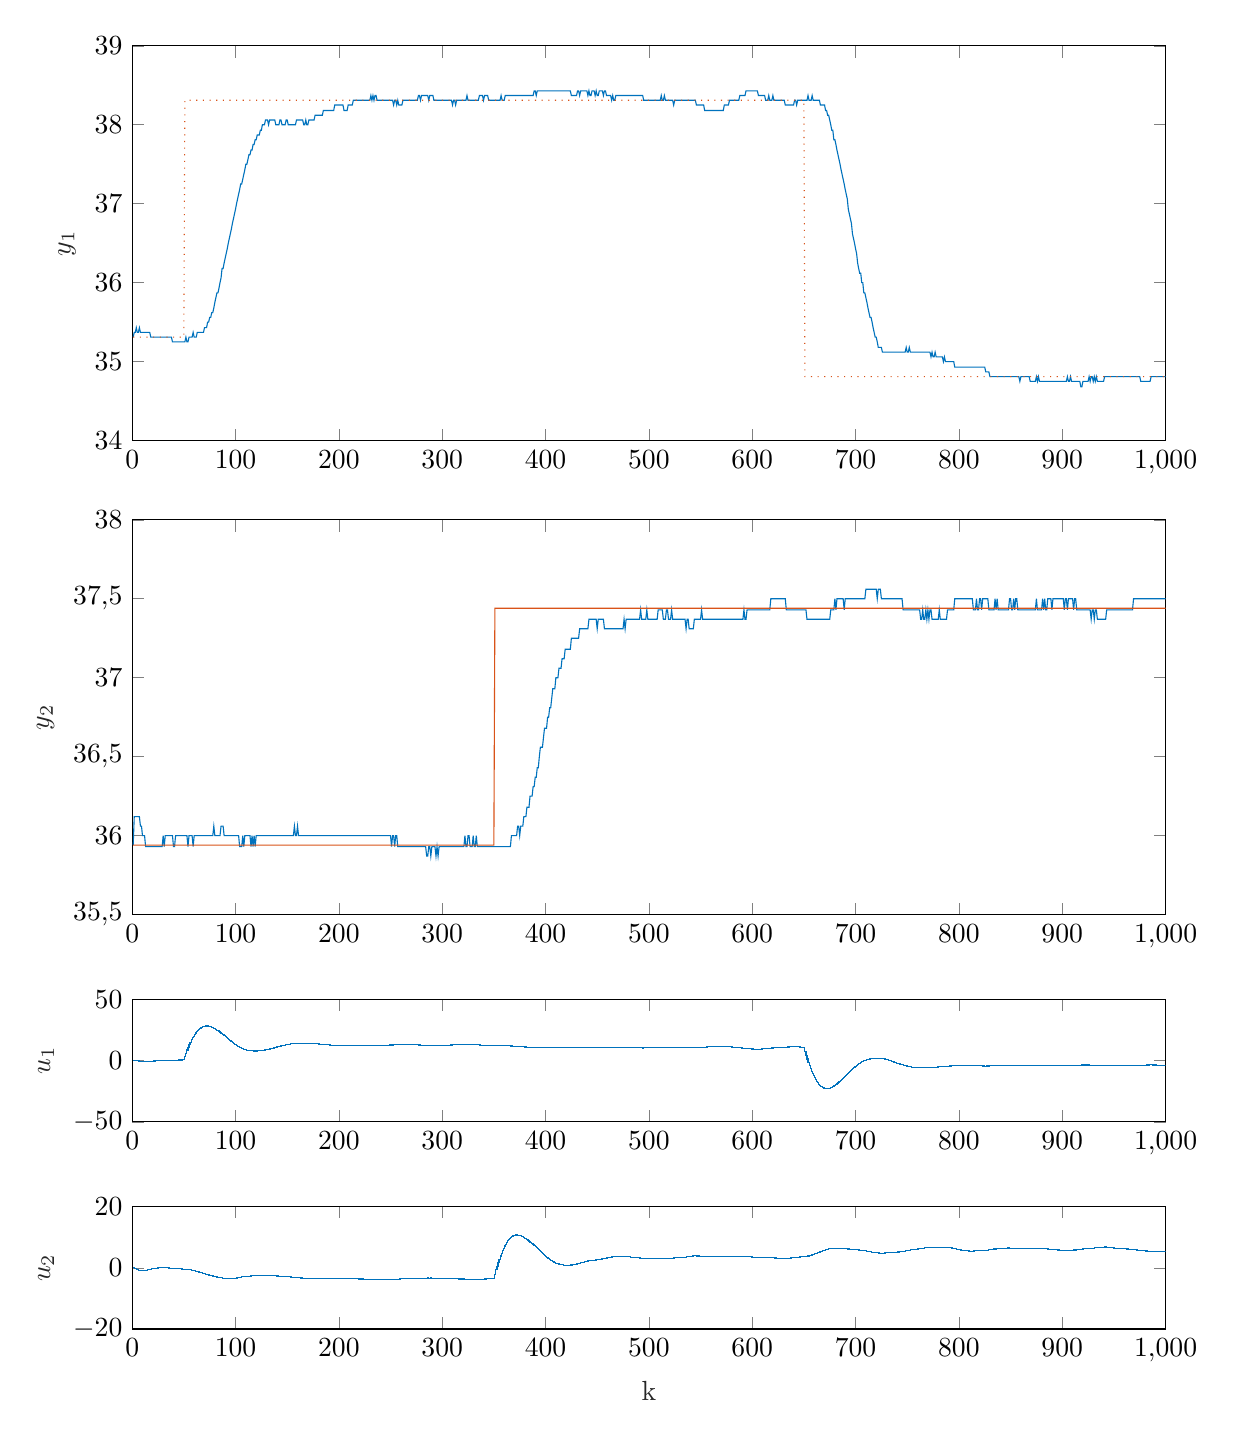
\begin{tikzpicture}

\begin{axis}[%
width=5.167in,
height=0.612in,
at={(0.646in,0.494in)},
scale only axis,
xmin=0,
xmax=1000,
xtick={0,100,200,300,400,500,600,700,800,900,1000},
xlabel style={font=\color{white!15!black}},
xlabel={k},
ymin=-20,
ymax=20,
ytick={-20,0,20},
ylabel style={font=\color{white!15!black}},
ylabel={$\text{u}_\text{2}$},
axis background/.style={fill=white}
]
\addplot[const plot, color=mycolor1, forget plot] table[row sep=crcr] {%
1	0\\
2	-0.17399\\
3	-0.33616\\
4	-0.48682\\
5	-0.62638\\
6	-0.75538\\
7	-0.87411\\
8	-0.92494\\
9	-0.9703\\
10	-0.9524\\
11	-0.93341\\
12	-0.91344\\
13	-0.82491\\
14	-0.74014\\
15	-0.65908\\
16	-0.58168\\
17	-0.50789\\
18	-0.43774\\
19	-0.37128\\
20	-0.30843\\
21	-0.24911\\
22	-0.19324\\
23	-0.14078\\
24	-0.091699\\
25	-0.045991\\
26	-0.0036543\\
27	0.035303\\
28	0.070873\\
29	0.10306\\
30	0.064163\\
31	0.094143\\
32	0.052967\\
33	0.012921\\
34	-0.02606\\
35	-0.064019\\
36	-0.10098\\
37	-0.13695\\
38	-0.17193\\
39	-0.20601\\
40	-0.17156\\
41	-0.14076\\
42	-0.18109\\
43	-0.22014\\
44	-0.25785\\
45	-0.29416\\
46	-0.32903\\
47	-0.36239\\
48	-0.3942\\
49	-0.4244\\
50	-0.45298\\
51	-0.48523\\
52	-0.52602\\
53	-0.57462\\
54	-0.56277\\
55	-0.62961\\
56	-0.70204\\
57	-0.77946\\
58	-0.86129\\
59	-0.87919\\
60	-0.97257\\
61	-1.0686\\
62	-1.1669\\
63	-1.2668\\
64	-1.3678\\
65	-1.4695\\
66	-1.5715\\
67	-1.6735\\
68	-1.7751\\
69	-1.876\\
70	-1.9759\\
71	-2.0743\\
72	-2.1711\\
73	-2.2659\\
74	-2.3583\\
75	-2.4481\\
76	-2.535\\
77	-2.6186\\
78	-2.6988\\
79	-2.8332\\
80	-2.9017\\
81	-2.966\\
82	-3.0259\\
83	-3.0813\\
84	-3.1321\\
85	-3.1782\\
86	-3.2775\\
87	-3.3679\\
88	-3.4497\\
89	-3.4649\\
90	-3.4757\\
91	-3.4822\\
92	-3.4844\\
93	-3.4825\\
94	-3.4766\\
95	-3.4669\\
96	-3.4536\\
97	-3.4368\\
98	-3.4169\\
99	-3.3939\\
100	-3.3683\\
101	-3.3402\\
102	-3.3098\\
103	-3.2775\\
104	-3.1757\\
105	-3.077\\
106	-2.9816\\
107	-2.9573\\
108	-2.8644\\
109	-2.843\\
110	-2.8209\\
111	-2.7985\\
112	-2.776\\
113	-2.7536\\
114	-2.7317\\
115	-2.6426\\
116	-2.6266\\
117	-2.5438\\
118	-2.5342\\
119	-2.458\\
120	-2.4551\\
121	-2.4533\\
122	-2.4527\\
123	-2.4534\\
124	-2.4555\\
125	-2.4591\\
126	-2.464\\
127	-2.4702\\
128	-2.4778\\
129	-2.4867\\
130	-2.4969\\
131	-2.5083\\
132	-2.521\\
133	-2.5351\\
134	-2.5505\\
135	-2.567\\
136	-2.5848\\
137	-2.6036\\
138	-2.6234\\
139	-2.6443\\
140	-2.6663\\
141	-2.6893\\
142	-2.7131\\
143	-2.7377\\
144	-2.7626\\
145	-2.7881\\
146	-2.8141\\
147	-2.8405\\
148	-2.8672\\
149	-2.8941\\
150	-2.9209\\
151	-2.9476\\
152	-2.9744\\
153	-3.0011\\
154	-3.0276\\
155	-3.0539\\
156	-3.08\\
157	-3.1637\\
158	-3.1851\\
159	-3.2061\\
160	-3.2846\\
161	-3.3006\\
162	-3.316\\
163	-3.331\\
164	-3.3454\\
165	-3.3593\\
166	-3.3727\\
167	-3.3857\\
168	-3.3983\\
169	-3.4104\\
170	-3.4221\\
171	-3.4333\\
172	-3.4439\\
173	-3.454\\
174	-3.4634\\
175	-3.4724\\
176	-3.4808\\
177	-3.4886\\
178	-3.4958\\
179	-3.5024\\
180	-3.5084\\
181	-3.5139\\
182	-3.5191\\
183	-3.5238\\
184	-3.5283\\
185	-3.5323\\
186	-3.536\\
187	-3.5393\\
188	-3.5422\\
189	-3.545\\
190	-3.5475\\
191	-3.55\\
192	-3.5523\\
193	-3.5546\\
194	-3.5569\\
195	-3.5592\\
196	-3.5615\\
197	-3.5636\\
198	-3.5657\\
199	-3.5677\\
200	-3.5698\\
201	-3.5719\\
202	-3.574\\
203	-3.5763\\
204	-3.5788\\
205	-3.5815\\
206	-3.5847\\
207	-3.5884\\
208	-3.5925\\
209	-3.5969\\
210	-3.6015\\
211	-3.6064\\
212	-3.6115\\
213	-3.6168\\
214	-3.6223\\
215	-3.6278\\
216	-3.6334\\
217	-3.6391\\
218	-3.6448\\
219	-3.6507\\
220	-3.6567\\
221	-3.6627\\
222	-3.6689\\
223	-3.6752\\
224	-3.6816\\
225	-3.6882\\
226	-3.6948\\
227	-3.7016\\
228	-3.7085\\
229	-3.7155\\
230	-3.7225\\
231	-3.7296\\
232	-3.7366\\
233	-3.7436\\
234	-3.7506\\
235	-3.7576\\
236	-3.7644\\
237	-3.7712\\
238	-3.7781\\
239	-3.7851\\
240	-3.7921\\
241	-3.7992\\
242	-3.8064\\
243	-3.8136\\
244	-3.8208\\
245	-3.8281\\
246	-3.8354\\
247	-3.8427\\
248	-3.85\\
249	-3.8574\\
250	-3.8647\\
251	-3.8043\\
252	-3.8162\\
253	-3.828\\
254	-3.772\\
255	-3.788\\
256	-3.8038\\
257	-3.7517\\
258	-3.7038\\
259	-3.6601\\
260	-3.6205\\
261	-3.5847\\
262	-3.5525\\
263	-3.5237\\
264	-3.4981\\
265	-3.4755\\
266	-3.4558\\
267	-3.4389\\
268	-3.4246\\
269	-3.4129\\
270	-3.4035\\
271	-3.3963\\
272	-3.3912\\
273	-3.3882\\
274	-3.3869\\
275	-3.3873\\
276	-3.3894\\
277	-3.3928\\
278	-3.3973\\
279	-3.4029\\
280	-3.4095\\
281	-3.4169\\
282	-3.4249\\
283	-3.4335\\
284	-3.4425\\
285	-3.3938\\
286	-3.3491\\
287	-3.3665\\
288	-3.3837\\
289	-3.3426\\
290	-3.363\\
291	-3.3828\\
292	-3.4021\\
293	-3.4208\\
294	-3.381\\
295	-3.4025\\
296	-3.3651\\
297	-3.3888\\
298	-3.4116\\
299	-3.4333\\
300	-3.4539\\
301	-3.4736\\
302	-3.4921\\
303	-3.5097\\
304	-3.5262\\
305	-3.5416\\
306	-3.556\\
307	-3.5694\\
308	-3.5817\\
309	-3.593\\
310	-3.6034\\
311	-3.613\\
312	-3.6215\\
313	-3.6292\\
314	-3.636\\
315	-3.6419\\
316	-3.6469\\
317	-3.6511\\
318	-3.6544\\
319	-3.6568\\
320	-3.6585\\
321	-3.6595\\
322	-3.7274\\
323	-3.7225\\
324	-3.717\\
325	-3.7787\\
326	-3.8355\\
327	-3.8199\\
328	-3.8044\\
329	-3.7889\\
330	-3.8412\\
331	-3.8214\\
332	-3.802\\
333	-3.8506\\
334	-3.8274\\
335	-3.8047\\
336	-3.7826\\
337	-3.7608\\
338	-3.7395\\
339	-3.7186\\
340	-3.6983\\
341	-3.6787\\
342	-3.6595\\
343	-3.6409\\
344	-3.6229\\
345	-3.6056\\
346	-3.5891\\
347	-3.5735\\
348	-3.5587\\
349	-3.5447\\
350	-3.5317\\
351	-2.0687\\
352	-0.70327\\
353	0.56786\\
354	1.748\\
355	2.8406\\
356	3.8488\\
357	4.776\\
358	5.6255\\
359	6.4004\\
360	7.1038\\
361	7.7389\\
362	8.3091\\
363	8.8172\\
364	9.2664\\
365	9.6594\\
366	9.9993\\
367	10.221\\
368	10.4\\
369	10.538\\
370	10.638\\
371	10.703\\
372	10.734\\
373	10.678\\
374	10.599\\
375	10.557\\
376	10.435\\
377	10.298\\
378	10.15\\
379	9.9333\\
380	9.7139\\
381	9.4936\\
382	9.2166\\
383	8.9467\\
384	8.6859\\
385	8.368\\
386	8.0667\\
387	7.7831\\
388	7.4603\\
389	7.1611\\
390	6.828\\
391	6.5233\\
392	6.1891\\
393	5.8873\\
394	5.5499\\
395	5.1907\\
396	4.8709\\
397	4.5894\\
398	4.2872\\
399	3.967\\
400	3.6893\\
401	3.4526\\
402	3.1873\\
403	2.9639\\
404	2.7223\\
405	2.5225\\
406	2.3041\\
407	2.0689\\
408	1.8765\\
409	1.7243\\
410	1.5422\\
411	1.4\\
412	1.2951\\
413	1.1669\\
414	1.0749\\
415	1.0164\\
416	0.93082\\
417	0.87761\\
418	0.85418\\
419	0.80002\\
420	0.77459\\
421	0.7754\\
422	0.80006\\
423	0.84624\\
424	0.91174\\
425	0.92659\\
426	0.96088\\
427	1.0125\\
428	1.0795\\
429	1.1599\\
430	1.2519\\
431	1.3539\\
432	1.4645\\
433	1.5238\\
434	1.5925\\
435	1.6691\\
436	1.7523\\
437	1.8408\\
438	1.9334\\
439	2.0289\\
440	2.1265\\
441	2.2251\\
442	2.2658\\
443	2.3097\\
444	2.356\\
445	2.4041\\
446	2.4534\\
447	2.5032\\
448	2.5531\\
449	2.6025\\
450	2.709\\
451	2.7523\\
452	2.7943\\
453	2.8348\\
454	2.8737\\
455	2.9107\\
456	2.9457\\
457	3.0365\\
458	3.1214\\
459	3.2003\\
460	3.2733\\
461	3.3406\\
462	3.4022\\
463	3.4585\\
464	3.5094\\
465	3.5553\\
466	3.5963\\
467	3.6326\\
468	3.6645\\
469	3.6924\\
470	3.7164\\
471	3.7368\\
472	3.7539\\
473	3.7679\\
474	3.779\\
475	3.7874\\
476	3.7354\\
477	3.743\\
478	3.6905\\
479	3.64\\
480	3.5914\\
481	3.545\\
482	3.5008\\
483	3.4589\\
484	3.4193\\
485	3.3822\\
486	3.3474\\
487	3.3152\\
488	3.2854\\
489	3.2583\\
490	3.2336\\
491	3.2116\\
492	3.134\\
493	3.1209\\
494	3.1102\\
495	3.1018\\
496	3.0954\\
497	3.0911\\
498	3.0308\\
499	3.0342\\
500	3.0395\\
501	3.0463\\
502	3.0547\\
503	3.0645\\
504	3.0756\\
505	3.0879\\
506	3.1013\\
507	3.1157\\
508	3.1309\\
509	3.0888\\
510	3.0512\\
511	3.0178\\
512	2.9886\\
513	2.9632\\
514	2.9993\\
515	3.035\\
516	3.0701\\
517	3.0464\\
518	3.0257\\
519	3.0659\\
520	3.1048\\
521	3.1424\\
522	3.1207\\
523	3.1595\\
524	3.1966\\
525	3.2321\\
526	3.2661\\
527	3.2985\\
528	3.3294\\
529	3.3588\\
530	3.3866\\
531	3.4129\\
532	3.4378\\
533	3.4611\\
534	3.4829\\
535	3.5032\\
536	3.5801\\
537	3.5937\\
538	3.6061\\
539	3.6752\\
540	3.7393\\
541	3.7986\\
542	3.8531\\
543	3.9032\\
544	3.8909\\
545	3.8783\\
546	3.8654\\
547	3.8523\\
548	3.8388\\
549	3.8252\\
550	3.8115\\
551	3.7397\\
552	3.7299\\
553	3.72\\
554	3.7101\\
555	3.7\\
556	3.6899\\
557	3.6799\\
558	3.6699\\
559	3.6602\\
560	3.6507\\
561	3.6415\\
562	3.6328\\
563	3.6246\\
564	3.6169\\
565	3.6099\\
566	3.6036\\
567	3.598\\
568	3.5932\\
569	3.5891\\
570	3.5858\\
571	3.5833\\
572	3.5816\\
573	3.5808\\
574	3.5809\\
575	3.5819\\
576	3.5839\\
577	3.5867\\
578	3.5904\\
579	3.595\\
580	3.6006\\
581	3.607\\
582	3.6141\\
583	3.622\\
584	3.6305\\
585	3.6396\\
586	3.6492\\
587	3.6593\\
588	3.6699\\
589	3.681\\
590	3.6926\\
591	3.7046\\
592	3.6589\\
593	3.6755\\
594	3.6922\\
595	3.6511\\
596	3.6141\\
597	3.5809\\
598	3.5513\\
599	3.5253\\
600	3.5024\\
601	3.4827\\
602	3.4659\\
603	3.4518\\
604	3.4403\\
605	3.4312\\
606	3.4242\\
607	3.4191\\
608	3.4158\\
609	3.4141\\
610	3.414\\
611	3.4152\\
612	3.4178\\
613	3.4214\\
614	3.4258\\
615	3.4311\\
616	3.4371\\
617	3.4439\\
618	3.3834\\
619	3.3279\\
620	3.2771\\
621	3.2308\\
622	3.1888\\
623	3.1506\\
624	3.1162\\
625	3.0854\\
626	3.0578\\
627	3.0333\\
628	3.0117\\
629	2.9929\\
630	2.9766\\
631	2.9626\\
632	2.9508\\
633	3.0086\\
634	3.0636\\
635	3.1159\\
636	3.1654\\
637	3.2123\\
638	3.2566\\
639	3.2983\\
640	3.3375\\
641	3.3743\\
642	3.4088\\
643	3.441\\
644	3.4709\\
645	3.4986\\
646	3.5241\\
647	3.5475\\
648	3.5687\\
649	3.588\\
650	3.6051\\
651	3.6265\\
652	3.658\\
653	3.7568\\
654	3.8603\\
655	3.968\\
656	4.0793\\
657	4.1935\\
658	4.3103\\
659	4.4291\\
660	4.5495\\
661	4.6709\\
662	4.793\\
663	4.9153\\
664	5.0375\\
665	5.1593\\
666	5.2802\\
667	5.3997\\
668	5.5177\\
669	5.6338\\
670	5.7478\\
671	5.8594\\
672	5.9682\\
673	6.0739\\
674	6.1763\\
675	6.275\\
676	6.3118\\
677	6.3481\\
678	6.3837\\
679	6.4181\\
680	6.3832\\
681	6.4187\\
682	6.3843\\
683	6.3519\\
684	6.3212\\
685	6.2918\\
686	6.2633\\
687	6.2356\\
688	6.2084\\
689	6.2493\\
690	6.2181\\
691	6.1871\\
692	6.1563\\
693	6.1254\\
694	6.0943\\
695	6.063\\
696	6.0316\\
697	6\\
698	5.968\\
699	5.9358\\
700	5.9034\\
701	5.871\\
702	5.8383\\
703	5.8055\\
704	5.7725\\
705	5.7396\\
706	5.7068\\
707	5.6742\\
708	5.6418\\
709	5.6098\\
710	5.5202\\
711	5.435\\
712	5.3541\\
713	5.2775\\
714	5.205\\
715	5.1367\\
716	5.0726\\
717	5.0125\\
718	4.9563\\
719	4.9039\\
720	4.8553\\
721	4.8684\\
722	4.8232\\
723	4.7817\\
724	4.7438\\
725	4.7677\\
726	4.7914\\
727	4.8148\\
728	4.8382\\
729	4.8615\\
730	4.885\\
731	4.9086\\
732	4.9325\\
733	4.9566\\
734	4.9809\\
735	5.0054\\
736	5.0301\\
737	5.055\\
738	5.08\\
739	5.105\\
740	5.13\\
741	5.1549\\
742	5.1796\\
743	5.2042\\
744	5.2285\\
745	5.2524\\
746	5.3436\\
747	5.4298\\
748	5.5111\\
749	5.5878\\
750	5.6599\\
751	5.7274\\
752	5.7906\\
753	5.8496\\
754	5.9044\\
755	5.9551\\
756	6.0018\\
757	6.0448\\
758	6.084\\
759	6.1197\\
760	6.1519\\
761	6.1809\\
762	6.2066\\
763	6.2874\\
764	6.3613\\
765	6.3707\\
766	6.4358\\
767	6.4947\\
768	6.4898\\
769	6.5412\\
770	6.5293\\
771	6.5741\\
772	6.556\\
773	6.5371\\
774	6.5754\\
775	6.6093\\
776	6.639\\
777	6.6648\\
778	6.687\\
779	6.7059\\
780	6.7215\\
781	6.6762\\
782	6.6902\\
783	6.7017\\
784	6.7108\\
785	6.7178\\
786	6.7228\\
787	6.7261\\
788	6.7279\\
789	6.6702\\
790	6.6152\\
791	6.563\\
792	6.5136\\
793	6.467\\
794	6.4232\\
795	6.3823\\
796	6.2764\\
797	6.1777\\
798	6.086\\
799	6.0011\\
800	5.923\\
801	5.8513\\
802	5.786\\
803	5.7269\\
804	5.6737\\
805	5.6264\\
806	5.5846\\
807	5.5483\\
808	5.5171\\
809	5.4909\\
810	5.4695\\
811	5.4527\\
812	5.4401\\
813	5.4317\\
814	5.4947\\
815	5.5568\\
816	5.6179\\
817	5.6102\\
818	5.6734\\
819	5.7351\\
820	5.7274\\
821	5.7226\\
822	5.7879\\
823	5.7833\\
824	5.7808\\
825	5.7802\\
826	5.7812\\
827	5.7834\\
828	5.7866\\
829	5.8584\\
830	5.9262\\
831	5.9899\\
832	6.0496\\
833	6.1052\\
834	6.1568\\
835	6.1369\\
836	6.1852\\
837	6.162\\
838	6.2072\\
839	6.2485\\
840	6.2862\\
841	6.3202\\
842	6.3508\\
843	6.378\\
844	6.4021\\
845	6.4232\\
846	6.4413\\
847	6.4567\\
848	6.4694\\
849	6.4119\\
850	6.3566\\
851	6.3712\\
852	6.3834\\
853	6.3258\\
854	6.3383\\
855	6.2811\\
856	6.2267\\
857	6.2426\\
858	6.2566\\
859	6.2689\\
860	6.2794\\
861	6.2886\\
862	6.2965\\
863	6.3034\\
864	6.3092\\
865	6.3141\\
866	6.3183\\
867	6.3218\\
868	6.3249\\
869	6.3273\\
870	6.3292\\
871	6.3306\\
872	6.3315\\
873	6.3321\\
874	6.3323\\
875	6.2647\\
876	6.2692\\
877	6.2734\\
878	6.2774\\
879	6.281\\
880	6.2843\\
881	6.2196\\
882	6.2269\\
883	6.1661\\
884	6.1772\\
885	6.1878\\
886	6.1302\\
887	6.0767\\
888	6.0272\\
889	5.9814\\
890	6.0071\\
891	5.964\\
892	5.9246\\
893	5.8885\\
894	5.8558\\
895	5.8262\\
896	5.7996\\
897	5.7759\\
898	5.7549\\
899	5.7365\\
900	5.7206\\
901	5.707\\
902	5.7633\\
903	5.7494\\
904	5.7376\\
905	5.7955\\
906	5.7831\\
907	5.7726\\
908	5.7638\\
909	5.7566\\
910	5.7508\\
911	5.814\\
912	5.806\\
913	5.7992\\
914	5.8611\\
915	5.9195\\
916	5.9742\\
917	6.0254\\
918	6.0729\\
919	6.1168\\
920	6.1572\\
921	6.1943\\
922	6.2281\\
923	6.2588\\
924	6.2865\\
925	6.3111\\
926	6.3329\\
927	6.3521\\
928	6.4266\\
929	6.4369\\
930	6.4448\\
931	6.5086\\
932	6.5084\\
933	6.5063\\
934	6.5605\\
935	6.609\\
936	6.6522\\
937	6.6902\\
938	6.7234\\
939	6.7521\\
940	6.7764\\
941	6.7968\\
942	6.8136\\
943	6.7691\\
944	6.7253\\
945	6.6824\\
946	6.6404\\
947	6.5995\\
948	6.5597\\
949	6.5211\\
950	6.4838\\
951	6.4478\\
952	6.4132\\
953	6.3801\\
954	6.3484\\
955	6.3183\\
956	6.2897\\
957	6.2627\\
958	6.2374\\
959	6.2137\\
960	6.1916\\
961	6.1713\\
962	6.1527\\
963	6.1358\\
964	6.1205\\
965	6.107\\
966	6.095\\
967	6.0846\\
968	6.0757\\
969	6.0006\\
970	5.9313\\
971	5.8677\\
972	5.8095\\
973	5.7564\\
974	5.7083\\
975	5.665\\
976	5.6259\\
977	5.5909\\
978	5.5597\\
979	5.5322\\
980	5.508\\
981	5.487\\
982	5.469\\
983	5.4538\\
984	5.4412\\
985	5.431\\
986	5.4232\\
987	5.4177\\
988	5.4142\\
989	5.4128\\
990	5.413\\
991	5.4149\\
992	5.4182\\
993	5.4227\\
994	5.4282\\
995	5.4346\\
996	5.4418\\
997	5.4496\\
998	5.4578\\
999	5.4662\\
1000	5.4749\\
};
\end{axis}

\begin{axis}[%
width=5.167in,
height=0.612in,
at={(0.646in,1.53in)},
scale only axis,
xmin=0,
xmax=1000,
xtick={0,100,200,300,400,500,600,700,800,900,1000},
ymin=-50,
ymax=50,
ytick={-50,0,50},
ylabel style={font=\color{white!15!black}},
ylabel={$\text{u}_\text{1}$},
axis background/.style={fill=white}
]
\addplot[const plot, color=mycolor1, forget plot] table[row sep=crcr] {%
1	0\\
2	-0.057711\\
3	-0.11093\\
4	-0.21787\\
5	-0.25877\\
6	-0.29584\\
7	-0.38727\\
8	-0.41342\\
9	-0.43657\\
10	-0.45699\\
11	-0.47492\\
12	-0.49049\\
13	-0.50395\\
14	-0.51553\\
15	-0.52535\\
16	-0.53349\\
17	-0.54007\\
18	-0.48714\\
19	-0.43671\\
20	-0.38872\\
21	-0.34313\\
22	-0.2999\\
23	-0.259\\
24	-0.2204\\
25	-0.18408\\
26	-0.15004\\
27	-0.11825\\
28	-0.088725\\
29	-0.061446\\
30	-0.036279\\
31	-0.013213\\
32	0.0077642\\
33	0.026799\\
34	0.043908\\
35	0.059115\\
36	0.07245\\
37	0.083948\\
38	0.093655\\
39	0.15966\\
40	0.22001\\
41	0.2748\\
42	0.3244\\
43	0.36915\\
44	0.4093\\
45	0.44507\\
46	0.4767\\
47	0.50442\\
48	0.52845\\
49	0.54903\\
50	0.56638\\
51	3.4823\\
52	6.1439\\
53	8.6779\\
54	11.029\\
55	13.146\\
56	15.098\\
57	16.89\\
58	18.531\\
59	19.967\\
60	21.326\\
61	22.55\\
62	23.648\\
63	24.566\\
64	25.373\\
65	26.073\\
66	26.674\\
67	27.18\\
68	27.596\\
69	27.928\\
70	28.123\\
71	28.249\\
72	28.309\\
73	28.243\\
74	28.128\\
75	27.912\\
76	27.662\\
77	27.325\\
78	26.97\\
79	26.542\\
80	26.041\\
81	25.486\\
82	24.884\\
83	24.301\\
84	23.682\\
85	23.025\\
86	22.346\\
87	21.593\\
88	20.892\\
89	20.176\\
90	19.46\\
91	18.748\\
92	18.043\\
93	17.341\\
94	16.653\\
95	15.983\\
96	15.332\\
97	14.694\\
98	14.079\\
99	13.489\\
100	12.925\\
101	12.377\\
102	11.857\\
103	11.364\\
104	10.899\\
105	10.449\\
106	10.085\\
107	9.7422\\
108	9.4206\\
109	9.119\\
110	8.8269\\
111	8.6114\\
112	8.4091\\
113	8.2189\\
114	8.0975\\
115	7.9814\\
116	7.9275\\
117	7.8629\\
118	7.8548\\
119	7.8403\\
120	7.8762\\
121	7.8999\\
122	7.9687\\
123	8.0779\\
124	8.1649\\
125	8.2876\\
126	8.3739\\
127	8.492\\
128	8.6382\\
129	8.7505\\
130	8.8873\\
131	9.0452\\
132	9.279\\
133	9.4655\\
134	9.6641\\
135	9.8721\\
136	10.087\\
137	10.306\\
138	10.528\\
139	10.809\\
140	11.085\\
141	11.354\\
142	11.616\\
143	11.811\\
144	12\\
145	12.241\\
146	12.47\\
147	12.687\\
148	12.892\\
149	13.027\\
150	13.152\\
151	13.326\\
152	13.487\\
153	13.635\\
154	13.77\\
155	13.892\\
156	14.002\\
157	14.1\\
158	14.186\\
159	14.203\\
160	14.214\\
161	14.217\\
162	14.215\\
163	14.208\\
164	14.195\\
165	14.178\\
166	14.215\\
167	14.245\\
168	14.21\\
169	14.231\\
170	14.246\\
171	14.198\\
172	14.15\\
173	14.102\\
174	14.054\\
175	14.008\\
176	13.962\\
177	13.86\\
178	13.764\\
179	13.673\\
180	13.589\\
181	13.511\\
182	13.439\\
183	13.373\\
184	13.313\\
185	13.202\\
186	13.1\\
187	13.009\\
188	12.926\\
189	12.853\\
190	12.789\\
191	12.734\\
192	12.687\\
193	12.649\\
194	12.618\\
195	12.594\\
196	12.51\\
197	12.437\\
198	12.374\\
199	12.322\\
200	12.279\\
201	12.246\\
202	12.22\\
203	12.203\\
204	12.193\\
205	12.257\\
206	12.324\\
207	12.391\\
208	12.46\\
209	12.462\\
210	12.468\\
211	12.479\\
212	12.494\\
213	12.512\\
214	12.475\\
215	12.445\\
216	12.42\\
217	12.401\\
218	12.387\\
219	12.378\\
220	12.373\\
221	12.371\\
222	12.373\\
223	12.377\\
224	12.384\\
225	12.393\\
226	12.404\\
227	12.416\\
228	12.43\\
229	12.445\\
230	12.461\\
231	12.42\\
232	12.441\\
233	12.404\\
234	12.429\\
235	12.397\\
236	12.368\\
237	12.4\\
238	12.431\\
239	12.462\\
240	12.492\\
241	12.521\\
242	12.549\\
243	12.575\\
244	12.601\\
245	12.625\\
246	12.648\\
247	12.67\\
248	12.69\\
249	12.709\\
250	12.727\\
251	12.744\\
252	12.759\\
253	12.831\\
254	12.839\\
255	12.847\\
256	12.911\\
257	12.913\\
258	12.971\\
259	13.024\\
260	13.073\\
261	13.117\\
262	13.099\\
263	13.081\\
264	13.062\\
265	13.043\\
266	13.024\\
267	13.005\\
268	12.986\\
269	12.967\\
270	12.949\\
271	12.931\\
272	12.913\\
273	12.895\\
274	12.878\\
275	12.861\\
276	12.845\\
277	12.771\\
278	12.702\\
279	12.696\\
280	12.632\\
281	12.572\\
282	12.517\\
283	12.466\\
284	12.419\\
285	12.375\\
286	12.336\\
287	12.358\\
288	12.323\\
289	12.29\\
290	12.261\\
291	12.236\\
292	12.272\\
293	12.307\\
294	12.341\\
295	12.374\\
296	12.406\\
297	12.437\\
298	12.468\\
299	12.497\\
300	12.526\\
301	12.553\\
302	12.58\\
303	12.605\\
304	12.63\\
305	12.653\\
306	12.675\\
307	12.695\\
308	12.714\\
309	12.732\\
310	12.807\\
311	12.818\\
312	12.828\\
313	12.895\\
314	12.898\\
315	12.901\\
316	12.902\\
317	12.902\\
318	12.902\\
319	12.9\\
320	12.898\\
321	12.895\\
322	12.891\\
323	12.887\\
324	12.824\\
325	12.822\\
326	12.82\\
327	12.818\\
328	12.815\\
329	12.811\\
330	12.808\\
331	12.804\\
332	12.8\\
333	12.796\\
334	12.792\\
335	12.787\\
336	12.725\\
337	12.667\\
338	12.612\\
339	12.561\\
340	12.572\\
341	12.525\\
342	12.481\\
343	12.44\\
344	12.403\\
345	12.427\\
346	12.45\\
347	12.473\\
348	12.494\\
349	12.515\\
350	12.536\\
351	12.553\\
352	12.564\\
353	12.569\\
354	12.569\\
355	12.565\\
356	12.556\\
357	12.485\\
358	12.472\\
359	12.455\\
360	12.434\\
361	12.353\\
362	12.273\\
363	12.193\\
364	12.115\\
365	12.038\\
366	11.963\\
367	11.889\\
368	11.817\\
369	11.748\\
370	11.68\\
371	11.614\\
372	11.55\\
373	11.488\\
374	11.429\\
375	11.373\\
376	11.319\\
377	11.267\\
378	11.218\\
379	11.172\\
380	11.129\\
381	11.089\\
382	11.052\\
383	11.018\\
384	10.987\\
385	10.959\\
386	10.935\\
387	10.913\\
388	10.894\\
389	10.82\\
390	10.752\\
391	10.749\\
392	10.69\\
393	10.638\\
394	10.591\\
395	10.55\\
396	10.514\\
397	10.484\\
398	10.458\\
399	10.437\\
400	10.42\\
401	10.407\\
402	10.398\\
403	10.393\\
404	10.39\\
405	10.39\\
406	10.393\\
407	10.398\\
408	10.406\\
409	10.415\\
410	10.426\\
411	10.439\\
412	10.452\\
413	10.467\\
414	10.482\\
415	10.497\\
416	10.513\\
417	10.529\\
418	10.545\\
419	10.56\\
420	10.575\\
421	10.589\\
422	10.603\\
423	10.615\\
424	10.627\\
425	10.695\\
426	10.758\\
427	10.816\\
428	10.87\\
429	10.918\\
430	10.962\\
431	10.942\\
432	10.922\\
433	10.96\\
434	10.935\\
435	10.909\\
436	10.883\\
437	10.856\\
438	10.829\\
439	10.802\\
440	10.774\\
441	10.804\\
442	10.771\\
443	10.797\\
444	10.819\\
445	10.779\\
446	10.74\\
447	10.701\\
448	10.721\\
449	10.68\\
450	10.697\\
451	10.712\\
452	10.666\\
453	10.621\\
454	10.577\\
455	10.535\\
456	10.552\\
457	10.509\\
458	10.467\\
459	10.485\\
460	10.5\\
461	10.514\\
462	10.524\\
463	10.533\\
464	10.598\\
465	10.6\\
466	10.658\\
467	10.71\\
468	10.7\\
469	10.689\\
470	10.677\\
471	10.664\\
472	10.65\\
473	10.636\\
474	10.622\\
475	10.607\\
476	10.592\\
477	10.576\\
478	10.56\\
479	10.545\\
480	10.529\\
481	10.513\\
482	10.498\\
483	10.482\\
484	10.466\\
485	10.451\\
486	10.436\\
487	10.421\\
488	10.407\\
489	10.392\\
490	10.379\\
491	10.365\\
492	10.353\\
493	10.34\\
494	10.329\\
495	10.375\\
496	10.419\\
497	10.459\\
498	10.496\\
499	10.53\\
500	10.561\\
501	10.59\\
502	10.615\\
503	10.639\\
504	10.659\\
505	10.678\\
506	10.694\\
507	10.708\\
508	10.72\\
509	10.73\\
510	10.738\\
511	10.745\\
512	10.692\\
513	10.699\\
514	10.705\\
515	10.651\\
516	10.658\\
517	10.662\\
518	10.666\\
519	10.668\\
520	10.669\\
521	10.669\\
522	10.667\\
523	10.665\\
524	10.72\\
525	10.712\\
526	10.703\\
527	10.694\\
528	10.685\\
529	10.675\\
530	10.665\\
531	10.655\\
532	10.645\\
533	10.635\\
534	10.625\\
535	10.614\\
536	10.604\\
537	10.594\\
538	10.584\\
539	10.575\\
540	10.565\\
541	10.555\\
542	10.546\\
543	10.536\\
544	10.527\\
545	10.519\\
546	10.569\\
547	10.615\\
548	10.658\\
549	10.699\\
550	10.736\\
551	10.77\\
552	10.802\\
553	10.831\\
554	10.925\\
555	11.012\\
556	11.093\\
557	11.167\\
558	11.235\\
559	11.297\\
560	11.354\\
561	11.405\\
562	11.451\\
563	11.492\\
564	11.528\\
565	11.56\\
566	11.588\\
567	11.612\\
568	11.631\\
569	11.648\\
570	11.661\\
571	11.67\\
572	11.677\\
573	11.614\\
574	11.553\\
575	11.494\\
576	11.437\\
577	11.382\\
578	11.272\\
579	11.168\\
580	11.07\\
581	10.978\\
582	10.893\\
583	10.813\\
584	10.739\\
585	10.672\\
586	10.609\\
587	10.553\\
588	10.444\\
589	10.344\\
590	10.252\\
591	10.17\\
592	10.096\\
593	10.03\\
594	9.9137\\
595	9.8088\\
596	9.7149\\
597	9.6315\\
598	9.5582\\
599	9.4944\\
600	9.4396\\
601	9.3932\\
602	9.3548\\
603	9.3239\\
604	9.2999\\
605	9.2824\\
606	9.3289\\
607	9.3769\\
608	9.4262\\
609	9.4765\\
610	9.5274\\
611	9.5785\\
612	9.6297\\
613	9.7386\\
614	9.843\\
615	9.9429\\
616	9.98\\
617	10.074\\
618	10.163\\
619	10.248\\
620	10.269\\
621	10.348\\
622	10.421\\
623	10.489\\
624	10.551\\
625	10.609\\
626	10.661\\
627	10.708\\
628	10.75\\
629	10.787\\
630	10.82\\
631	10.847\\
632	10.929\\
633	11.002\\
634	11.066\\
635	11.124\\
636	11.174\\
637	11.217\\
638	11.253\\
639	11.283\\
640	11.308\\
641	11.269\\
642	11.229\\
643	11.246\\
644	11.201\\
645	11.155\\
646	11.109\\
647	11.064\\
648	11.019\\
649	10.974\\
650	10.93\\
651	7.5024\\
652	4.3013\\
653	1.3193\\
654	-1.5092\\
655	-4.0719\\
656	-6.4382\\
657	-8.6157\\
658	-10.67\\
659	-12.487\\
660	-14.138\\
661	-15.629\\
662	-16.968\\
663	-18.161\\
664	-19.215\\
665	-20.137\\
666	-20.876\\
667	-21.499\\
668	-22.015\\
669	-22.427\\
670	-22.744\\
671	-22.902\\
672	-22.981\\
673	-22.93\\
674	-22.816\\
675	-22.59\\
676	-22.261\\
677	-21.83\\
678	-21.375\\
679	-20.788\\
680	-20.196\\
681	-19.548\\
682	-18.842\\
683	-18.098\\
684	-17.323\\
685	-16.524\\
686	-15.7\\
687	-14.867\\
688	-14.031\\
689	-13.197\\
690	-12.361\\
691	-11.538\\
692	-10.732\\
693	-9.8787\\
694	-9.0532\\
695	-8.2581\\
696	-7.4957\\
697	-6.6998\\
698	-5.9439\\
699	-5.2289\\
700	-4.5453\\
701	-3.9036\\
702	-3.2456\\
703	-2.6228\\
704	-2.0447\\
705	-1.5682\\
706	-1.0719\\
707	-0.67421\\
708	-0.2438\\
709	0.090886\\
710	0.39394\\
711	0.66751\\
712	0.92338\\
713	1.1534\\
714	1.3599\\
715	1.487\\
716	1.5991\\
717	1.7078\\
718	1.8051\\
719	1.8931\\
720	1.9159\\
721	1.9373\\
722	1.9689\\
723	1.9442\\
724	1.8688\\
725	1.7479\\
726	1.6447\\
727	1.5022\\
728	1.325\\
729	1.1179\\
730	0.88517\\
731	0.63081\\
732	0.35865\\
733	0.072309\\
734	-0.22489\\
735	-0.52984\\
736	-0.83967\\
737	-1.1517\\
738	-1.4636\\
739	-1.773\\
740	-2.0781\\
741	-2.3769\\
742	-2.6679\\
743	-2.9497\\
744	-3.2209\\
745	-3.4806\\
746	-3.7279\\
747	-3.9622\\
748	-4.1829\\
749	-4.4475\\
750	-4.6359\\
751	-4.8098\\
752	-5.0273\\
753	-5.1684\\
754	-5.2953\\
755	-5.4083\\
756	-5.5078\\
757	-5.5941\\
758	-5.6678\\
759	-5.7294\\
760	-5.7795\\
761	-5.8187\\
762	-5.8478\\
763	-5.8675\\
764	-5.8788\\
765	-5.8821\\
766	-5.8783\\
767	-5.8682\\
768	-5.8524\\
769	-5.8317\\
770	-5.8067\\
771	-5.7782\\
772	-5.7468\\
773	-5.6551\\
774	-5.6236\\
775	-5.5331\\
776	-5.446\\
777	-5.4206\\
778	-5.3374\\
779	-5.2587\\
780	-5.1848\\
781	-5.1157\\
782	-5.0517\\
783	-4.9929\\
784	-4.9395\\
785	-4.8336\\
786	-4.795\\
787	-4.7037\\
788	-4.6217\\
789	-4.5486\\
790	-4.484\\
791	-4.4278\\
792	-4.3798\\
793	-4.3396\\
794	-4.3069\\
795	-4.2815\\
796	-4.1952\\
797	-4.1198\\
798	-4.0548\\
799	-3.9996\\
800	-3.9538\\
801	-3.9168\\
802	-3.8882\\
803	-3.8674\\
804	-3.854\\
805	-3.8474\\
806	-3.8471\\
807	-3.8527\\
808	-3.8636\\
809	-3.8795\\
810	-3.8997\\
811	-3.9239\\
812	-3.9517\\
813	-3.9825\\
814	-4.0163\\
815	-4.0526\\
816	-4.091\\
817	-4.1312\\
818	-4.1727\\
819	-4.2153\\
820	-4.2586\\
821	-4.3022\\
822	-4.3459\\
823	-4.3895\\
824	-4.4325\\
825	-4.4748\\
826	-4.4582\\
827	-4.4444\\
828	-4.4331\\
829	-4.4241\\
830	-4.3594\\
831	-4.3005\\
832	-4.2472\\
833	-4.1991\\
834	-4.1559\\
835	-4.1172\\
836	-4.0828\\
837	-4.0522\\
838	-4.0254\\
839	-4.0022\\
840	-3.9825\\
841	-3.9659\\
842	-3.9524\\
843	-3.9417\\
844	-3.9336\\
845	-3.9281\\
846	-3.925\\
847	-3.9242\\
848	-3.9254\\
849	-3.9284\\
850	-3.933\\
851	-3.9391\\
852	-3.9467\\
853	-3.9555\\
854	-3.9654\\
855	-3.9762\\
856	-3.9877\\
857	-3.9997\\
858	-4.0124\\
859	-3.9676\\
860	-3.985\\
861	-4.0025\\
862	-4.02\\
863	-4.0373\\
864	-4.0544\\
865	-4.0712\\
866	-4.0875\\
867	-4.1034\\
868	-4.1188\\
869	-4.0755\\
870	-4.0354\\
871	-3.9983\\
872	-3.9641\\
873	-3.9327\\
874	-3.9038\\
875	-3.9352\\
876	-3.907\\
877	-3.9391\\
878	-3.9115\\
879	-3.8862\\
880	-3.8629\\
881	-3.8415\\
882	-3.8219\\
883	-3.804\\
884	-3.7877\\
885	-3.7731\\
886	-3.7599\\
887	-3.7479\\
888	-3.7372\\
889	-3.7275\\
890	-3.7191\\
891	-3.7118\\
892	-3.7055\\
893	-3.7\\
894	-3.6953\\
895	-3.6913\\
896	-3.688\\
897	-3.6852\\
898	-3.683\\
899	-3.6813\\
900	-3.68\\
901	-3.679\\
902	-3.6785\\
903	-3.6783\\
904	-3.6783\\
905	-3.7366\\
906	-3.7332\\
907	-3.73\\
908	-3.7849\\
909	-3.7779\\
910	-3.7712\\
911	-3.7647\\
912	-3.7585\\
913	-3.7524\\
914	-3.7464\\
915	-3.7407\\
916	-3.7353\\
917	-3.7301\\
918	-3.6574\\
919	-3.5894\\
920	-3.5935\\
921	-3.5975\\
922	-3.6012\\
923	-3.6047\\
924	-3.608\\
925	-3.611\\
926	-3.6719\\
927	-3.6705\\
928	-3.7273\\
929	-3.7801\\
930	-3.7711\\
931	-3.8204\\
932	-3.808\\
933	-3.854\\
934	-3.8385\\
935	-3.8237\\
936	-3.8094\\
937	-3.7958\\
938	-3.7827\\
939	-3.7702\\
940	-3.7582\\
941	-3.8047\\
942	-3.8478\\
943	-3.8874\\
944	-3.9236\\
945	-3.9564\\
946	-3.9861\\
947	-4.0128\\
948	-4.0365\\
949	-4.0574\\
950	-4.0757\\
951	-4.0915\\
952	-4.105\\
953	-4.1162\\
954	-4.1254\\
955	-4.1326\\
956	-4.1381\\
957	-4.1418\\
958	-4.1439\\
959	-4.1445\\
960	-4.1437\\
961	-4.1416\\
962	-4.1384\\
963	-4.1341\\
964	-4.1288\\
965	-4.1227\\
966	-4.1158\\
967	-4.1083\\
968	-4.1003\\
969	-4.0918\\
970	-4.0827\\
971	-4.0731\\
972	-4.0631\\
973	-4.0529\\
974	-4.0425\\
975	-4.0321\\
976	-3.9635\\
977	-3.899\\
978	-3.8382\\
979	-3.7813\\
980	-3.7281\\
981	-3.6785\\
982	-3.6325\\
983	-3.5899\\
984	-3.5507\\
985	-3.5147\\
986	-3.5399\\
987	-3.5643\\
988	-3.588\\
989	-3.6108\\
990	-3.6328\\
991	-3.6542\\
992	-3.6748\\
993	-3.6946\\
994	-3.7138\\
995	-3.7323\\
996	-3.7501\\
997	-3.7672\\
998	-3.7837\\
999	-3.7994\\
1000	-3.8143\\
};
\end{axis}

\begin{axis}[%
width=5.167in,
height=1.974in,
at={(0.646in,2.566in)},
scale only axis,
xmin=0,
xmax=1000,
xtick={0,100,200,300,400,500,600,700,800,900,1000},
ymin=35.5,
ymax=38,
ytick={35.5,36,36.5,37,37.5,38},
yticklabels={{35,5},{36},{36,5},{37},{37,5},{38}},
ylabel style={font=\color{white!15!black}},
ylabel={$\text{y}_\text{2}$},
axis background/.style={fill=white}
]
\addplot [color=mycolor1, forget plot]
  table[row sep=crcr]{%
1	35.94\\
2	36.12\\
3	36.12\\
4	36.12\\
5	36.12\\
6	36.12\\
7	36.12\\
8	36.06\\
9	36.06\\
10	36\\
11	36\\
12	36\\
13	35.93\\
14	35.93\\
15	35.93\\
16	35.93\\
17	35.93\\
18	35.93\\
19	35.93\\
20	35.93\\
21	35.93\\
22	35.93\\
23	35.93\\
24	35.93\\
25	35.93\\
26	35.93\\
27	35.93\\
28	35.93\\
29	35.93\\
30	36\\
31	35.93\\
32	36\\
33	36\\
34	36\\
35	36\\
36	36\\
37	36\\
38	36\\
39	36\\
40	35.93\\
41	35.93\\
42	36\\
43	36\\
44	36\\
45	36\\
46	36\\
47	36\\
48	36\\
49	36\\
50	36\\
51	36\\
52	36\\
53	36\\
54	35.93\\
55	36\\
56	36\\
57	36\\
58	36\\
59	35.93\\
60	36\\
61	36\\
62	36\\
63	36\\
64	36\\
65	36\\
66	36\\
67	36\\
68	36\\
69	36\\
70	36\\
71	36\\
72	36\\
73	36\\
74	36\\
75	36\\
76	36\\
77	36\\
78	36\\
79	36.06\\
80	36\\
81	36\\
82	36\\
83	36\\
84	36\\
85	36\\
86	36.06\\
87	36.06\\
88	36.06\\
89	36\\
90	36\\
91	36\\
92	36\\
93	36\\
94	36\\
95	36\\
96	36\\
97	36\\
98	36\\
99	36\\
100	36\\
101	36\\
102	36\\
103	36\\
104	35.93\\
105	35.93\\
106	35.93\\
107	36\\
108	35.93\\
109	36\\
110	36\\
111	36\\
112	36\\
113	36\\
114	36\\
115	35.93\\
116	36\\
117	35.93\\
118	36\\
119	35.93\\
120	36\\
121	36\\
122	36\\
123	36\\
124	36\\
125	36\\
126	36\\
127	36\\
128	36\\
129	36\\
130	36\\
131	36\\
132	36\\
133	36\\
134	36\\
135	36\\
136	36\\
137	36\\
138	36\\
139	36\\
140	36\\
141	36\\
142	36\\
143	36\\
144	36\\
145	36\\
146	36\\
147	36\\
148	36\\
149	36\\
150	36\\
151	36\\
152	36\\
153	36\\
154	36\\
155	36\\
156	36\\
157	36.06\\
158	36\\
159	36\\
160	36.06\\
161	36\\
162	36\\
163	36\\
164	36\\
165	36\\
166	36\\
167	36\\
168	36\\
169	36\\
170	36\\
171	36\\
172	36\\
173	36\\
174	36\\
175	36\\
176	36\\
177	36\\
178	36\\
179	36\\
180	36\\
181	36\\
182	36\\
183	36\\
184	36\\
185	36\\
186	36\\
187	36\\
188	36\\
189	36\\
190	36\\
191	36\\
192	36\\
193	36\\
194	36\\
195	36\\
196	36\\
197	36\\
198	36\\
199	36\\
200	36\\
201	36\\
202	36\\
203	36\\
204	36\\
205	36\\
206	36\\
207	36\\
208	36\\
209	36\\
210	36\\
211	36\\
212	36\\
213	36\\
214	36\\
215	36\\
216	36\\
217	36\\
218	36\\
219	36\\
220	36\\
221	36\\
222	36\\
223	36\\
224	36\\
225	36\\
226	36\\
227	36\\
228	36\\
229	36\\
230	36\\
231	36\\
232	36\\
233	36\\
234	36\\
235	36\\
236	36\\
237	36\\
238	36\\
239	36\\
240	36\\
241	36\\
242	36\\
243	36\\
244	36\\
245	36\\
246	36\\
247	36\\
248	36\\
249	36\\
250	36\\
251	35.93\\
252	36\\
253	36\\
254	35.93\\
255	36\\
256	36\\
257	35.93\\
258	35.93\\
259	35.93\\
260	35.93\\
261	35.93\\
262	35.93\\
263	35.93\\
264	35.93\\
265	35.93\\
266	35.93\\
267	35.93\\
268	35.93\\
269	35.93\\
270	35.93\\
271	35.93\\
272	35.93\\
273	35.93\\
274	35.93\\
275	35.93\\
276	35.93\\
277	35.93\\
278	35.93\\
279	35.93\\
280	35.93\\
281	35.93\\
282	35.93\\
283	35.93\\
284	35.93\\
285	35.87\\
286	35.87\\
287	35.93\\
288	35.93\\
289	35.87\\
290	35.93\\
291	35.93\\
292	35.93\\
293	35.93\\
294	35.87\\
295	35.93\\
296	35.87\\
297	35.93\\
298	35.93\\
299	35.93\\
300	35.93\\
301	35.93\\
302	35.93\\
303	35.93\\
304	35.93\\
305	35.93\\
306	35.93\\
307	35.93\\
308	35.93\\
309	35.93\\
310	35.93\\
311	35.93\\
312	35.93\\
313	35.93\\
314	35.93\\
315	35.93\\
316	35.93\\
317	35.93\\
318	35.93\\
319	35.93\\
320	35.93\\
321	35.93\\
322	36\\
323	35.93\\
324	35.93\\
325	36\\
326	36\\
327	35.93\\
328	35.93\\
329	35.93\\
330	36\\
331	35.93\\
332	35.93\\
333	36\\
334	35.93\\
335	35.93\\
336	35.93\\
337	35.93\\
338	35.93\\
339	35.93\\
340	35.93\\
341	35.93\\
342	35.93\\
343	35.93\\
344	35.93\\
345	35.93\\
346	35.93\\
347	35.93\\
348	35.93\\
349	35.93\\
350	35.93\\
351	35.93\\
352	35.93\\
353	35.93\\
354	35.93\\
355	35.93\\
356	35.93\\
357	35.93\\
358	35.93\\
359	35.93\\
360	35.93\\
361	35.93\\
362	35.93\\
363	35.93\\
364	35.93\\
365	35.93\\
366	35.93\\
367	36\\
368	36\\
369	36\\
370	36\\
371	36\\
372	36\\
373	36.06\\
374	36.06\\
375	36\\
376	36.06\\
377	36.06\\
378	36.06\\
379	36.12\\
380	36.12\\
381	36.12\\
382	36.18\\
383	36.18\\
384	36.18\\
385	36.25\\
386	36.25\\
387	36.25\\
388	36.31\\
389	36.31\\
390	36.37\\
391	36.37\\
392	36.43\\
393	36.43\\
394	36.5\\
395	36.56\\
396	36.56\\
397	36.56\\
398	36.62\\
399	36.68\\
400	36.68\\
401	36.68\\
402	36.75\\
403	36.75\\
404	36.81\\
405	36.81\\
406	36.87\\
407	36.93\\
408	36.93\\
409	36.93\\
410	37\\
411	37\\
412	37\\
413	37.06\\
414	37.06\\
415	37.06\\
416	37.12\\
417	37.12\\
418	37.12\\
419	37.18\\
420	37.18\\
421	37.18\\
422	37.18\\
423	37.18\\
424	37.18\\
425	37.25\\
426	37.25\\
427	37.25\\
428	37.25\\
429	37.25\\
430	37.25\\
431	37.25\\
432	37.25\\
433	37.31\\
434	37.31\\
435	37.31\\
436	37.31\\
437	37.31\\
438	37.31\\
439	37.31\\
440	37.31\\
441	37.31\\
442	37.37\\
443	37.37\\
444	37.37\\
445	37.37\\
446	37.37\\
447	37.37\\
448	37.37\\
449	37.37\\
450	37.31\\
451	37.37\\
452	37.37\\
453	37.37\\
454	37.37\\
455	37.37\\
456	37.37\\
457	37.31\\
458	37.31\\
459	37.31\\
460	37.31\\
461	37.31\\
462	37.31\\
463	37.31\\
464	37.31\\
465	37.31\\
466	37.31\\
467	37.31\\
468	37.31\\
469	37.31\\
470	37.31\\
471	37.31\\
472	37.31\\
473	37.31\\
474	37.31\\
475	37.31\\
476	37.37\\
477	37.31\\
478	37.37\\
479	37.37\\
480	37.37\\
481	37.37\\
482	37.37\\
483	37.37\\
484	37.37\\
485	37.37\\
486	37.37\\
487	37.37\\
488	37.37\\
489	37.37\\
490	37.37\\
491	37.37\\
492	37.43\\
493	37.37\\
494	37.37\\
495	37.37\\
496	37.37\\
497	37.37\\
498	37.43\\
499	37.37\\
500	37.37\\
501	37.37\\
502	37.37\\
503	37.37\\
504	37.37\\
505	37.37\\
506	37.37\\
507	37.37\\
508	37.37\\
509	37.43\\
510	37.43\\
511	37.43\\
512	37.43\\
513	37.43\\
514	37.37\\
515	37.37\\
516	37.37\\
517	37.43\\
518	37.43\\
519	37.37\\
520	37.37\\
521	37.37\\
522	37.43\\
523	37.37\\
524	37.37\\
525	37.37\\
526	37.37\\
527	37.37\\
528	37.37\\
529	37.37\\
530	37.37\\
531	37.37\\
532	37.37\\
533	37.37\\
534	37.37\\
535	37.37\\
536	37.31\\
537	37.37\\
538	37.37\\
539	37.31\\
540	37.31\\
541	37.31\\
542	37.31\\
543	37.31\\
544	37.37\\
545	37.37\\
546	37.37\\
547	37.37\\
548	37.37\\
549	37.37\\
550	37.37\\
551	37.43\\
552	37.37\\
553	37.37\\
554	37.37\\
555	37.37\\
556	37.37\\
557	37.37\\
558	37.37\\
559	37.37\\
560	37.37\\
561	37.37\\
562	37.37\\
563	37.37\\
564	37.37\\
565	37.37\\
566	37.37\\
567	37.37\\
568	37.37\\
569	37.37\\
570	37.37\\
571	37.37\\
572	37.37\\
573	37.37\\
574	37.37\\
575	37.37\\
576	37.37\\
577	37.37\\
578	37.37\\
579	37.37\\
580	37.37\\
581	37.37\\
582	37.37\\
583	37.37\\
584	37.37\\
585	37.37\\
586	37.37\\
587	37.37\\
588	37.37\\
589	37.37\\
590	37.37\\
591	37.37\\
592	37.43\\
593	37.37\\
594	37.37\\
595	37.43\\
596	37.43\\
597	37.43\\
598	37.43\\
599	37.43\\
600	37.43\\
601	37.43\\
602	37.43\\
603	37.43\\
604	37.43\\
605	37.43\\
606	37.43\\
607	37.43\\
608	37.43\\
609	37.43\\
610	37.43\\
611	37.43\\
612	37.43\\
613	37.43\\
614	37.43\\
615	37.43\\
616	37.43\\
617	37.43\\
618	37.5\\
619	37.5\\
620	37.5\\
621	37.5\\
622	37.5\\
623	37.5\\
624	37.5\\
625	37.5\\
626	37.5\\
627	37.5\\
628	37.5\\
629	37.5\\
630	37.5\\
631	37.5\\
632	37.5\\
633	37.43\\
634	37.43\\
635	37.43\\
636	37.43\\
637	37.43\\
638	37.43\\
639	37.43\\
640	37.43\\
641	37.43\\
642	37.43\\
643	37.43\\
644	37.43\\
645	37.43\\
646	37.43\\
647	37.43\\
648	37.43\\
649	37.43\\
650	37.43\\
651	37.43\\
652	37.43\\
653	37.37\\
654	37.37\\
655	37.37\\
656	37.37\\
657	37.37\\
658	37.37\\
659	37.37\\
660	37.37\\
661	37.37\\
662	37.37\\
663	37.37\\
664	37.37\\
665	37.37\\
666	37.37\\
667	37.37\\
668	37.37\\
669	37.37\\
670	37.37\\
671	37.37\\
672	37.37\\
673	37.37\\
674	37.37\\
675	37.37\\
676	37.43\\
677	37.43\\
678	37.43\\
679	37.43\\
680	37.5\\
681	37.43\\
682	37.5\\
683	37.5\\
684	37.5\\
685	37.5\\
686	37.5\\
687	37.5\\
688	37.5\\
689	37.43\\
690	37.5\\
691	37.5\\
692	37.5\\
693	37.5\\
694	37.5\\
695	37.5\\
696	37.5\\
697	37.5\\
698	37.5\\
699	37.5\\
700	37.5\\
701	37.5\\
702	37.5\\
703	37.5\\
704	37.5\\
705	37.5\\
706	37.5\\
707	37.5\\
708	37.5\\
709	37.5\\
710	37.56\\
711	37.56\\
712	37.56\\
713	37.56\\
714	37.56\\
715	37.56\\
716	37.56\\
717	37.56\\
718	37.56\\
719	37.56\\
720	37.56\\
721	37.5\\
722	37.56\\
723	37.56\\
724	37.56\\
725	37.5\\
726	37.5\\
727	37.5\\
728	37.5\\
729	37.5\\
730	37.5\\
731	37.5\\
732	37.5\\
733	37.5\\
734	37.5\\
735	37.5\\
736	37.5\\
737	37.5\\
738	37.5\\
739	37.5\\
740	37.5\\
741	37.5\\
742	37.5\\
743	37.5\\
744	37.5\\
745	37.5\\
746	37.43\\
747	37.43\\
748	37.43\\
749	37.43\\
750	37.43\\
751	37.43\\
752	37.43\\
753	37.43\\
754	37.43\\
755	37.43\\
756	37.43\\
757	37.43\\
758	37.43\\
759	37.43\\
760	37.43\\
761	37.43\\
762	37.43\\
763	37.37\\
764	37.37\\
765	37.43\\
766	37.37\\
767	37.37\\
768	37.43\\
769	37.37\\
770	37.43\\
771	37.37\\
772	37.43\\
773	37.43\\
774	37.37\\
775	37.37\\
776	37.37\\
777	37.37\\
778	37.37\\
779	37.37\\
780	37.37\\
781	37.43\\
782	37.37\\
783	37.37\\
784	37.37\\
785	37.37\\
786	37.37\\
787	37.37\\
788	37.37\\
789	37.43\\
790	37.43\\
791	37.43\\
792	37.43\\
793	37.43\\
794	37.43\\
795	37.43\\
796	37.5\\
797	37.5\\
798	37.5\\
799	37.5\\
800	37.5\\
801	37.5\\
802	37.5\\
803	37.5\\
804	37.5\\
805	37.5\\
806	37.5\\
807	37.5\\
808	37.5\\
809	37.5\\
810	37.5\\
811	37.5\\
812	37.5\\
813	37.5\\
814	37.43\\
815	37.43\\
816	37.43\\
817	37.5\\
818	37.43\\
819	37.43\\
820	37.5\\
821	37.5\\
822	37.43\\
823	37.5\\
824	37.5\\
825	37.5\\
826	37.5\\
827	37.5\\
828	37.5\\
829	37.43\\
830	37.43\\
831	37.43\\
832	37.43\\
833	37.43\\
834	37.43\\
835	37.5\\
836	37.43\\
837	37.5\\
838	37.43\\
839	37.43\\
840	37.43\\
841	37.43\\
842	37.43\\
843	37.43\\
844	37.43\\
845	37.43\\
846	37.43\\
847	37.43\\
848	37.43\\
849	37.5\\
850	37.5\\
851	37.43\\
852	37.43\\
853	37.5\\
854	37.43\\
855	37.5\\
856	37.5\\
857	37.43\\
858	37.43\\
859	37.43\\
860	37.43\\
861	37.43\\
862	37.43\\
863	37.43\\
864	37.43\\
865	37.43\\
866	37.43\\
867	37.43\\
868	37.43\\
869	37.43\\
870	37.43\\
871	37.43\\
872	37.43\\
873	37.43\\
874	37.43\\
875	37.5\\
876	37.43\\
877	37.43\\
878	37.43\\
879	37.43\\
880	37.43\\
881	37.5\\
882	37.43\\
883	37.5\\
884	37.43\\
885	37.43\\
886	37.5\\
887	37.5\\
888	37.5\\
889	37.5\\
890	37.43\\
891	37.5\\
892	37.5\\
893	37.5\\
894	37.5\\
895	37.5\\
896	37.5\\
897	37.5\\
898	37.5\\
899	37.5\\
900	37.5\\
901	37.5\\
902	37.43\\
903	37.5\\
904	37.5\\
905	37.43\\
906	37.5\\
907	37.5\\
908	37.5\\
909	37.5\\
910	37.5\\
911	37.43\\
912	37.5\\
913	37.5\\
914	37.43\\
915	37.43\\
916	37.43\\
917	37.43\\
918	37.43\\
919	37.43\\
920	37.43\\
921	37.43\\
922	37.43\\
923	37.43\\
924	37.43\\
925	37.43\\
926	37.43\\
927	37.43\\
928	37.37\\
929	37.43\\
930	37.43\\
931	37.37\\
932	37.43\\
933	37.43\\
934	37.37\\
935	37.37\\
936	37.37\\
937	37.37\\
938	37.37\\
939	37.37\\
940	37.37\\
941	37.37\\
942	37.37\\
943	37.43\\
944	37.43\\
945	37.43\\
946	37.43\\
947	37.43\\
948	37.43\\
949	37.43\\
950	37.43\\
951	37.43\\
952	37.43\\
953	37.43\\
954	37.43\\
955	37.43\\
956	37.43\\
957	37.43\\
958	37.43\\
959	37.43\\
960	37.43\\
961	37.43\\
962	37.43\\
963	37.43\\
964	37.43\\
965	37.43\\
966	37.43\\
967	37.43\\
968	37.43\\
969	37.5\\
970	37.5\\
971	37.5\\
972	37.5\\
973	37.5\\
974	37.5\\
975	37.5\\
976	37.5\\
977	37.5\\
978	37.5\\
979	37.5\\
980	37.5\\
981	37.5\\
982	37.5\\
983	37.5\\
984	37.5\\
985	37.5\\
986	37.5\\
987	37.5\\
988	37.5\\
989	37.5\\
990	37.5\\
991	37.5\\
992	37.5\\
993	37.5\\
994	37.5\\
995	37.5\\
996	37.5\\
997	37.5\\
998	37.5\\
999	37.5\\
1000	37.5\\
};
\addplot [color=mycolor2, forget plot]
  table[row sep=crcr]{%
1	35.94\\
2	35.94\\
3	35.94\\
4	35.94\\
5	35.94\\
6	35.94\\
7	35.94\\
8	35.94\\
9	35.94\\
10	35.94\\
11	35.94\\
12	35.94\\
13	35.94\\
14	35.94\\
15	35.94\\
16	35.94\\
17	35.94\\
18	35.94\\
19	35.94\\
20	35.94\\
21	35.94\\
22	35.94\\
23	35.94\\
24	35.94\\
25	35.94\\
26	35.94\\
27	35.94\\
28	35.94\\
29	35.94\\
30	35.94\\
31	35.94\\
32	35.94\\
33	35.94\\
34	35.94\\
35	35.94\\
36	35.94\\
37	35.94\\
38	35.94\\
39	35.94\\
40	35.94\\
41	35.94\\
42	35.94\\
43	35.94\\
44	35.94\\
45	35.94\\
46	35.94\\
47	35.94\\
48	35.94\\
49	35.94\\
50	35.94\\
51	35.94\\
52	35.94\\
53	35.94\\
54	35.94\\
55	35.94\\
56	35.94\\
57	35.94\\
58	35.94\\
59	35.94\\
60	35.94\\
61	35.94\\
62	35.94\\
63	35.94\\
64	35.94\\
65	35.94\\
66	35.94\\
67	35.94\\
68	35.94\\
69	35.94\\
70	35.94\\
71	35.94\\
72	35.94\\
73	35.94\\
74	35.94\\
75	35.94\\
76	35.94\\
77	35.94\\
78	35.94\\
79	35.94\\
80	35.94\\
81	35.94\\
82	35.94\\
83	35.94\\
84	35.94\\
85	35.94\\
86	35.94\\
87	35.94\\
88	35.94\\
89	35.94\\
90	35.94\\
91	35.94\\
92	35.94\\
93	35.94\\
94	35.94\\
95	35.94\\
96	35.94\\
97	35.94\\
98	35.94\\
99	35.94\\
100	35.94\\
101	35.94\\
102	35.94\\
103	35.94\\
104	35.94\\
105	35.94\\
106	35.94\\
107	35.94\\
108	35.94\\
109	35.94\\
110	35.94\\
111	35.94\\
112	35.94\\
113	35.94\\
114	35.94\\
115	35.94\\
116	35.94\\
117	35.94\\
118	35.94\\
119	35.94\\
120	35.94\\
121	35.94\\
122	35.94\\
123	35.94\\
124	35.94\\
125	35.94\\
126	35.94\\
127	35.94\\
128	35.94\\
129	35.94\\
130	35.94\\
131	35.94\\
132	35.94\\
133	35.94\\
134	35.94\\
135	35.94\\
136	35.94\\
137	35.94\\
138	35.94\\
139	35.94\\
140	35.94\\
141	35.94\\
142	35.94\\
143	35.94\\
144	35.94\\
145	35.94\\
146	35.94\\
147	35.94\\
148	35.94\\
149	35.94\\
150	35.94\\
151	35.94\\
152	35.94\\
153	35.94\\
154	35.94\\
155	35.94\\
156	35.94\\
157	35.94\\
158	35.94\\
159	35.94\\
160	35.94\\
161	35.94\\
162	35.94\\
163	35.94\\
164	35.94\\
165	35.94\\
166	35.94\\
167	35.94\\
168	35.94\\
169	35.94\\
170	35.94\\
171	35.94\\
172	35.94\\
173	35.94\\
174	35.94\\
175	35.94\\
176	35.94\\
177	35.94\\
178	35.94\\
179	35.94\\
180	35.94\\
181	35.94\\
182	35.94\\
183	35.94\\
184	35.94\\
185	35.94\\
186	35.94\\
187	35.94\\
188	35.94\\
189	35.94\\
190	35.94\\
191	35.94\\
192	35.94\\
193	35.94\\
194	35.94\\
195	35.94\\
196	35.94\\
197	35.94\\
198	35.94\\
199	35.94\\
200	35.94\\
201	35.94\\
202	35.94\\
203	35.94\\
204	35.94\\
205	35.94\\
206	35.94\\
207	35.94\\
208	35.94\\
209	35.94\\
210	35.94\\
211	35.94\\
212	35.94\\
213	35.94\\
214	35.94\\
215	35.94\\
216	35.94\\
217	35.94\\
218	35.94\\
219	35.94\\
220	35.94\\
221	35.94\\
222	35.94\\
223	35.94\\
224	35.94\\
225	35.94\\
226	35.94\\
227	35.94\\
228	35.94\\
229	35.94\\
230	35.94\\
231	35.94\\
232	35.94\\
233	35.94\\
234	35.94\\
235	35.94\\
236	35.94\\
237	35.94\\
238	35.94\\
239	35.94\\
240	35.94\\
241	35.94\\
242	35.94\\
243	35.94\\
244	35.94\\
245	35.94\\
246	35.94\\
247	35.94\\
248	35.94\\
249	35.94\\
250	35.94\\
251	35.94\\
252	35.94\\
253	35.94\\
254	35.94\\
255	35.94\\
256	35.94\\
257	35.94\\
258	35.94\\
259	35.94\\
260	35.94\\
261	35.94\\
262	35.94\\
263	35.94\\
264	35.94\\
265	35.94\\
266	35.94\\
267	35.94\\
268	35.94\\
269	35.94\\
270	35.94\\
271	35.94\\
272	35.94\\
273	35.94\\
274	35.94\\
275	35.94\\
276	35.94\\
277	35.94\\
278	35.94\\
279	35.94\\
280	35.94\\
281	35.94\\
282	35.94\\
283	35.94\\
284	35.94\\
285	35.94\\
286	35.94\\
287	35.94\\
288	35.94\\
289	35.94\\
290	35.94\\
291	35.94\\
292	35.94\\
293	35.94\\
294	35.94\\
295	35.94\\
296	35.94\\
297	35.94\\
298	35.94\\
299	35.94\\
300	35.94\\
301	35.94\\
302	35.94\\
303	35.94\\
304	35.94\\
305	35.94\\
306	35.94\\
307	35.94\\
308	35.94\\
309	35.94\\
310	35.94\\
311	35.94\\
312	35.94\\
313	35.94\\
314	35.94\\
315	35.94\\
316	35.94\\
317	35.94\\
318	35.94\\
319	35.94\\
320	35.94\\
321	35.94\\
322	35.94\\
323	35.94\\
324	35.94\\
325	35.94\\
326	35.94\\
327	35.94\\
328	35.94\\
329	35.94\\
330	35.94\\
331	35.94\\
332	35.94\\
333	35.94\\
334	35.94\\
335	35.94\\
336	35.94\\
337	35.94\\
338	35.94\\
339	35.94\\
340	35.94\\
341	35.94\\
342	35.94\\
343	35.94\\
344	35.94\\
345	35.94\\
346	35.94\\
347	35.94\\
348	35.94\\
349	35.94\\
350	35.94\\
351	37.44\\
352	37.44\\
353	37.44\\
354	37.44\\
355	37.44\\
356	37.44\\
357	37.44\\
358	37.44\\
359	37.44\\
360	37.44\\
361	37.44\\
362	37.44\\
363	37.44\\
364	37.44\\
365	37.44\\
366	37.44\\
367	37.44\\
368	37.44\\
369	37.44\\
370	37.44\\
371	37.44\\
372	37.44\\
373	37.44\\
374	37.44\\
375	37.44\\
376	37.44\\
377	37.44\\
378	37.44\\
379	37.44\\
380	37.44\\
381	37.44\\
382	37.44\\
383	37.44\\
384	37.44\\
385	37.44\\
386	37.44\\
387	37.44\\
388	37.44\\
389	37.44\\
390	37.44\\
391	37.44\\
392	37.44\\
393	37.44\\
394	37.44\\
395	37.44\\
396	37.44\\
397	37.44\\
398	37.44\\
399	37.44\\
400	37.44\\
401	37.44\\
402	37.44\\
403	37.44\\
404	37.44\\
405	37.44\\
406	37.44\\
407	37.44\\
408	37.44\\
409	37.44\\
410	37.44\\
411	37.44\\
412	37.44\\
413	37.44\\
414	37.44\\
415	37.44\\
416	37.44\\
417	37.44\\
418	37.44\\
419	37.44\\
420	37.44\\
421	37.44\\
422	37.44\\
423	37.44\\
424	37.44\\
425	37.44\\
426	37.44\\
427	37.44\\
428	37.44\\
429	37.44\\
430	37.44\\
431	37.44\\
432	37.44\\
433	37.44\\
434	37.44\\
435	37.44\\
436	37.44\\
437	37.44\\
438	37.44\\
439	37.44\\
440	37.44\\
441	37.44\\
442	37.44\\
443	37.44\\
444	37.44\\
445	37.44\\
446	37.44\\
447	37.44\\
448	37.44\\
449	37.44\\
450	37.44\\
451	37.44\\
452	37.44\\
453	37.44\\
454	37.44\\
455	37.44\\
456	37.44\\
457	37.44\\
458	37.44\\
459	37.44\\
460	37.44\\
461	37.44\\
462	37.44\\
463	37.44\\
464	37.44\\
465	37.44\\
466	37.44\\
467	37.44\\
468	37.44\\
469	37.44\\
470	37.44\\
471	37.44\\
472	37.44\\
473	37.44\\
474	37.44\\
475	37.44\\
476	37.44\\
477	37.44\\
478	37.44\\
479	37.44\\
480	37.44\\
481	37.44\\
482	37.44\\
483	37.44\\
484	37.44\\
485	37.44\\
486	37.44\\
487	37.44\\
488	37.44\\
489	37.44\\
490	37.44\\
491	37.44\\
492	37.44\\
493	37.44\\
494	37.44\\
495	37.44\\
496	37.44\\
497	37.44\\
498	37.44\\
499	37.44\\
500	37.44\\
501	37.44\\
502	37.44\\
503	37.44\\
504	37.44\\
505	37.44\\
506	37.44\\
507	37.44\\
508	37.44\\
509	37.44\\
510	37.44\\
511	37.44\\
512	37.44\\
513	37.44\\
514	37.44\\
515	37.44\\
516	37.44\\
517	37.44\\
518	37.44\\
519	37.44\\
520	37.44\\
521	37.44\\
522	37.44\\
523	37.44\\
524	37.44\\
525	37.44\\
526	37.44\\
527	37.44\\
528	37.44\\
529	37.44\\
530	37.44\\
531	37.44\\
532	37.44\\
533	37.44\\
534	37.44\\
535	37.44\\
536	37.44\\
537	37.44\\
538	37.44\\
539	37.44\\
540	37.44\\
541	37.44\\
542	37.44\\
543	37.44\\
544	37.44\\
545	37.44\\
546	37.44\\
547	37.44\\
548	37.44\\
549	37.44\\
550	37.44\\
551	37.44\\
552	37.44\\
553	37.44\\
554	37.44\\
555	37.44\\
556	37.44\\
557	37.44\\
558	37.44\\
559	37.44\\
560	37.44\\
561	37.44\\
562	37.44\\
563	37.44\\
564	37.44\\
565	37.44\\
566	37.44\\
567	37.44\\
568	37.44\\
569	37.44\\
570	37.44\\
571	37.44\\
572	37.44\\
573	37.44\\
574	37.44\\
575	37.44\\
576	37.44\\
577	37.44\\
578	37.44\\
579	37.44\\
580	37.44\\
581	37.44\\
582	37.44\\
583	37.44\\
584	37.44\\
585	37.44\\
586	37.44\\
587	37.44\\
588	37.44\\
589	37.44\\
590	37.44\\
591	37.44\\
592	37.44\\
593	37.44\\
594	37.44\\
595	37.44\\
596	37.44\\
597	37.44\\
598	37.44\\
599	37.44\\
600	37.44\\
601	37.44\\
602	37.44\\
603	37.44\\
604	37.44\\
605	37.44\\
606	37.44\\
607	37.44\\
608	37.44\\
609	37.44\\
610	37.44\\
611	37.44\\
612	37.44\\
613	37.44\\
614	37.44\\
615	37.44\\
616	37.44\\
617	37.44\\
618	37.44\\
619	37.44\\
620	37.44\\
621	37.44\\
622	37.44\\
623	37.44\\
624	37.44\\
625	37.44\\
626	37.44\\
627	37.44\\
628	37.44\\
629	37.44\\
630	37.44\\
631	37.44\\
632	37.44\\
633	37.44\\
634	37.44\\
635	37.44\\
636	37.44\\
637	37.44\\
638	37.44\\
639	37.44\\
640	37.44\\
641	37.44\\
642	37.44\\
643	37.44\\
644	37.44\\
645	37.44\\
646	37.44\\
647	37.44\\
648	37.44\\
649	37.44\\
650	37.44\\
651	37.44\\
652	37.44\\
653	37.44\\
654	37.44\\
655	37.44\\
656	37.44\\
657	37.44\\
658	37.44\\
659	37.44\\
660	37.44\\
661	37.44\\
662	37.44\\
663	37.44\\
664	37.44\\
665	37.44\\
666	37.44\\
667	37.44\\
668	37.44\\
669	37.44\\
670	37.44\\
671	37.44\\
672	37.44\\
673	37.44\\
674	37.44\\
675	37.44\\
676	37.44\\
677	37.44\\
678	37.44\\
679	37.44\\
680	37.44\\
681	37.44\\
682	37.44\\
683	37.44\\
684	37.44\\
685	37.44\\
686	37.44\\
687	37.44\\
688	37.44\\
689	37.44\\
690	37.44\\
691	37.44\\
692	37.44\\
693	37.44\\
694	37.44\\
695	37.44\\
696	37.44\\
697	37.44\\
698	37.44\\
699	37.44\\
700	37.44\\
701	37.44\\
702	37.44\\
703	37.44\\
704	37.44\\
705	37.44\\
706	37.44\\
707	37.44\\
708	37.44\\
709	37.44\\
710	37.44\\
711	37.44\\
712	37.44\\
713	37.44\\
714	37.44\\
715	37.44\\
716	37.44\\
717	37.44\\
718	37.44\\
719	37.44\\
720	37.44\\
721	37.44\\
722	37.44\\
723	37.44\\
724	37.44\\
725	37.44\\
726	37.44\\
727	37.44\\
728	37.44\\
729	37.44\\
730	37.44\\
731	37.44\\
732	37.44\\
733	37.44\\
734	37.44\\
735	37.44\\
736	37.44\\
737	37.44\\
738	37.44\\
739	37.44\\
740	37.44\\
741	37.44\\
742	37.44\\
743	37.44\\
744	37.44\\
745	37.44\\
746	37.44\\
747	37.44\\
748	37.44\\
749	37.44\\
750	37.44\\
751	37.44\\
752	37.44\\
753	37.44\\
754	37.44\\
755	37.44\\
756	37.44\\
757	37.44\\
758	37.44\\
759	37.44\\
760	37.44\\
761	37.44\\
762	37.44\\
763	37.44\\
764	37.44\\
765	37.44\\
766	37.44\\
767	37.44\\
768	37.44\\
769	37.44\\
770	37.44\\
771	37.44\\
772	37.44\\
773	37.44\\
774	37.44\\
775	37.44\\
776	37.44\\
777	37.44\\
778	37.44\\
779	37.44\\
780	37.44\\
781	37.44\\
782	37.44\\
783	37.44\\
784	37.44\\
785	37.44\\
786	37.44\\
787	37.44\\
788	37.44\\
789	37.44\\
790	37.44\\
791	37.44\\
792	37.44\\
793	37.44\\
794	37.44\\
795	37.44\\
796	37.44\\
797	37.44\\
798	37.44\\
799	37.44\\
800	37.44\\
801	37.44\\
802	37.44\\
803	37.44\\
804	37.44\\
805	37.44\\
806	37.44\\
807	37.44\\
808	37.44\\
809	37.44\\
810	37.44\\
811	37.44\\
812	37.44\\
813	37.44\\
814	37.44\\
815	37.44\\
816	37.44\\
817	37.44\\
818	37.44\\
819	37.44\\
820	37.44\\
821	37.44\\
822	37.44\\
823	37.44\\
824	37.44\\
825	37.44\\
826	37.44\\
827	37.44\\
828	37.44\\
829	37.44\\
830	37.44\\
831	37.44\\
832	37.44\\
833	37.44\\
834	37.44\\
835	37.44\\
836	37.44\\
837	37.44\\
838	37.44\\
839	37.44\\
840	37.44\\
841	37.44\\
842	37.44\\
843	37.44\\
844	37.44\\
845	37.44\\
846	37.44\\
847	37.44\\
848	37.44\\
849	37.44\\
850	37.44\\
851	37.44\\
852	37.44\\
853	37.44\\
854	37.44\\
855	37.44\\
856	37.44\\
857	37.44\\
858	37.44\\
859	37.44\\
860	37.44\\
861	37.44\\
862	37.44\\
863	37.44\\
864	37.44\\
865	37.44\\
866	37.44\\
867	37.44\\
868	37.44\\
869	37.44\\
870	37.44\\
871	37.44\\
872	37.44\\
873	37.44\\
874	37.44\\
875	37.44\\
876	37.44\\
877	37.44\\
878	37.44\\
879	37.44\\
880	37.44\\
881	37.44\\
882	37.44\\
883	37.44\\
884	37.44\\
885	37.44\\
886	37.44\\
887	37.44\\
888	37.44\\
889	37.44\\
890	37.44\\
891	37.44\\
892	37.44\\
893	37.44\\
894	37.44\\
895	37.44\\
896	37.44\\
897	37.44\\
898	37.44\\
899	37.44\\
900	37.44\\
901	37.44\\
902	37.44\\
903	37.44\\
904	37.44\\
905	37.44\\
906	37.44\\
907	37.44\\
908	37.44\\
909	37.44\\
910	37.44\\
911	37.44\\
912	37.44\\
913	37.44\\
914	37.44\\
915	37.44\\
916	37.44\\
917	37.44\\
918	37.44\\
919	37.44\\
920	37.44\\
921	37.44\\
922	37.44\\
923	37.44\\
924	37.44\\
925	37.44\\
926	37.44\\
927	37.44\\
928	37.44\\
929	37.44\\
930	37.44\\
931	37.44\\
932	37.44\\
933	37.44\\
934	37.44\\
935	37.44\\
936	37.44\\
937	37.44\\
938	37.44\\
939	37.44\\
940	37.44\\
941	37.44\\
942	37.44\\
943	37.44\\
944	37.44\\
945	37.44\\
946	37.44\\
947	37.44\\
948	37.44\\
949	37.44\\
950	37.44\\
951	37.44\\
952	37.44\\
953	37.44\\
954	37.44\\
955	37.44\\
956	37.44\\
957	37.44\\
958	37.44\\
959	37.44\\
960	37.44\\
961	37.44\\
962	37.44\\
963	37.44\\
964	37.44\\
965	37.44\\
966	37.44\\
967	37.44\\
968	37.44\\
969	37.44\\
970	37.44\\
971	37.44\\
972	37.44\\
973	37.44\\
974	37.44\\
975	37.44\\
976	37.44\\
977	37.44\\
978	37.44\\
979	37.44\\
980	37.44\\
981	37.44\\
982	37.44\\
983	37.44\\
984	37.44\\
985	37.44\\
986	37.44\\
987	37.44\\
988	37.44\\
989	37.44\\
990	37.44\\
991	37.44\\
992	37.44\\
993	37.44\\
994	37.44\\
995	37.44\\
996	37.44\\
997	37.44\\
998	37.44\\
999	37.44\\
1000	37.44\\
};
\end{axis}

\begin{axis}[%
width=5.167in,
height=1.974in,
at={(0.646in,4.936in)},
scale only axis,
xmin=0,
xmax=1000,
xtick={0,100,200,300,400,500,600,700,800,900,1000},
ymin=34,
ymax=39,
ytick={34,35,36,37,38,39},
ylabel style={font=\color{white!15!black}},
ylabel={$\text{y}_\text{1}$},
axis background/.style={fill=white}
]
\addplot [color=mycolor1, forget plot]
  table[row sep=crcr]{%
1	35.31\\
2	35.37\\
3	35.37\\
4	35.43\\
5	35.37\\
6	35.37\\
7	35.43\\
8	35.37\\
9	35.37\\
10	35.37\\
11	35.37\\
12	35.37\\
13	35.37\\
14	35.37\\
15	35.37\\
16	35.37\\
17	35.37\\
18	35.31\\
19	35.31\\
20	35.31\\
21	35.31\\
22	35.31\\
23	35.31\\
24	35.31\\
25	35.31\\
26	35.31\\
27	35.31\\
28	35.31\\
29	35.31\\
30	35.31\\
31	35.31\\
32	35.31\\
33	35.31\\
34	35.31\\
35	35.31\\
36	35.31\\
37	35.31\\
38	35.31\\
39	35.25\\
40	35.25\\
41	35.25\\
42	35.25\\
43	35.25\\
44	35.25\\
45	35.25\\
46	35.25\\
47	35.25\\
48	35.25\\
49	35.25\\
50	35.25\\
51	35.25\\
52	35.31\\
53	35.25\\
54	35.25\\
55	35.31\\
56	35.31\\
57	35.31\\
58	35.31\\
59	35.37\\
60	35.31\\
61	35.31\\
62	35.31\\
63	35.37\\
64	35.37\\
65	35.37\\
66	35.37\\
67	35.37\\
68	35.37\\
69	35.37\\
70	35.43\\
71	35.43\\
72	35.43\\
73	35.5\\
74	35.5\\
75	35.56\\
76	35.56\\
77	35.62\\
78	35.62\\
79	35.68\\
80	35.75\\
81	35.81\\
82	35.87\\
83	35.87\\
84	35.93\\
85	36\\
86	36.06\\
87	36.18\\
88	36.18\\
89	36.25\\
90	36.31\\
91	36.37\\
92	36.43\\
93	36.5\\
94	36.56\\
95	36.62\\
96	36.68\\
97	36.75\\
98	36.81\\
99	36.87\\
100	36.93\\
101	37\\
102	37.06\\
103	37.12\\
104	37.18\\
105	37.25\\
106	37.25\\
107	37.31\\
108	37.37\\
109	37.43\\
110	37.5\\
111	37.5\\
112	37.56\\
113	37.62\\
114	37.62\\
115	37.68\\
116	37.68\\
117	37.75\\
118	37.75\\
119	37.81\\
120	37.81\\
121	37.87\\
122	37.87\\
123	37.87\\
124	37.93\\
125	37.93\\
126	38\\
127	38\\
128	38\\
129	38.06\\
130	38.06\\
131	38.06\\
132	38\\
133	38.06\\
134	38.06\\
135	38.06\\
136	38.06\\
137	38.06\\
138	38.06\\
139	38\\
140	38\\
141	38\\
142	38\\
143	38.06\\
144	38.06\\
145	38\\
146	38\\
147	38\\
148	38\\
149	38.06\\
150	38.06\\
151	38\\
152	38\\
153	38\\
154	38\\
155	38\\
156	38\\
157	38\\
158	38\\
159	38.06\\
160	38.06\\
161	38.06\\
162	38.06\\
163	38.06\\
164	38.06\\
165	38.06\\
166	38\\
167	38\\
168	38.06\\
169	38\\
170	38\\
171	38.06\\
172	38.06\\
173	38.06\\
174	38.06\\
175	38.06\\
176	38.06\\
177	38.12\\
178	38.12\\
179	38.12\\
180	38.12\\
181	38.12\\
182	38.12\\
183	38.12\\
184	38.12\\
185	38.18\\
186	38.18\\
187	38.18\\
188	38.18\\
189	38.18\\
190	38.18\\
191	38.18\\
192	38.18\\
193	38.18\\
194	38.18\\
195	38.18\\
196	38.25\\
197	38.25\\
198	38.25\\
199	38.25\\
200	38.25\\
201	38.25\\
202	38.25\\
203	38.25\\
204	38.25\\
205	38.18\\
206	38.18\\
207	38.18\\
208	38.18\\
209	38.25\\
210	38.25\\
211	38.25\\
212	38.25\\
213	38.25\\
214	38.31\\
215	38.31\\
216	38.31\\
217	38.31\\
218	38.31\\
219	38.31\\
220	38.31\\
221	38.31\\
222	38.31\\
223	38.31\\
224	38.31\\
225	38.31\\
226	38.31\\
227	38.31\\
228	38.31\\
229	38.31\\
230	38.31\\
231	38.37\\
232	38.31\\
233	38.37\\
234	38.31\\
235	38.37\\
236	38.37\\
237	38.31\\
238	38.31\\
239	38.31\\
240	38.31\\
241	38.31\\
242	38.31\\
243	38.31\\
244	38.31\\
245	38.31\\
246	38.31\\
247	38.31\\
248	38.31\\
249	38.31\\
250	38.31\\
251	38.31\\
252	38.31\\
253	38.25\\
254	38.31\\
255	38.31\\
256	38.25\\
257	38.31\\
258	38.25\\
259	38.25\\
260	38.25\\
261	38.25\\
262	38.31\\
263	38.31\\
264	38.31\\
265	38.31\\
266	38.31\\
267	38.31\\
268	38.31\\
269	38.31\\
270	38.31\\
271	38.31\\
272	38.31\\
273	38.31\\
274	38.31\\
275	38.31\\
276	38.31\\
277	38.37\\
278	38.37\\
279	38.31\\
280	38.37\\
281	38.37\\
282	38.37\\
283	38.37\\
284	38.37\\
285	38.37\\
286	38.37\\
287	38.31\\
288	38.37\\
289	38.37\\
290	38.37\\
291	38.37\\
292	38.31\\
293	38.31\\
294	38.31\\
295	38.31\\
296	38.31\\
297	38.31\\
298	38.31\\
299	38.31\\
300	38.31\\
301	38.31\\
302	38.31\\
303	38.31\\
304	38.31\\
305	38.31\\
306	38.31\\
307	38.31\\
308	38.31\\
309	38.31\\
310	38.25\\
311	38.31\\
312	38.31\\
313	38.25\\
314	38.31\\
315	38.31\\
316	38.31\\
317	38.31\\
318	38.31\\
319	38.31\\
320	38.31\\
321	38.31\\
322	38.31\\
323	38.31\\
324	38.37\\
325	38.31\\
326	38.31\\
327	38.31\\
328	38.31\\
329	38.31\\
330	38.31\\
331	38.31\\
332	38.31\\
333	38.31\\
334	38.31\\
335	38.31\\
336	38.37\\
337	38.37\\
338	38.37\\
339	38.37\\
340	38.31\\
341	38.37\\
342	38.37\\
343	38.37\\
344	38.37\\
345	38.31\\
346	38.31\\
347	38.31\\
348	38.31\\
349	38.31\\
350	38.31\\
351	38.31\\
352	38.31\\
353	38.31\\
354	38.31\\
355	38.31\\
356	38.31\\
357	38.37\\
358	38.31\\
359	38.31\\
360	38.31\\
361	38.37\\
362	38.37\\
363	38.37\\
364	38.37\\
365	38.37\\
366	38.37\\
367	38.37\\
368	38.37\\
369	38.37\\
370	38.37\\
371	38.37\\
372	38.37\\
373	38.37\\
374	38.37\\
375	38.37\\
376	38.37\\
377	38.37\\
378	38.37\\
379	38.37\\
380	38.37\\
381	38.37\\
382	38.37\\
383	38.37\\
384	38.37\\
385	38.37\\
386	38.37\\
387	38.37\\
388	38.37\\
389	38.43\\
390	38.43\\
391	38.37\\
392	38.43\\
393	38.43\\
394	38.43\\
395	38.43\\
396	38.43\\
397	38.43\\
398	38.43\\
399	38.43\\
400	38.43\\
401	38.43\\
402	38.43\\
403	38.43\\
404	38.43\\
405	38.43\\
406	38.43\\
407	38.43\\
408	38.43\\
409	38.43\\
410	38.43\\
411	38.43\\
412	38.43\\
413	38.43\\
414	38.43\\
415	38.43\\
416	38.43\\
417	38.43\\
418	38.43\\
419	38.43\\
420	38.43\\
421	38.43\\
422	38.43\\
423	38.43\\
424	38.43\\
425	38.37\\
426	38.37\\
427	38.37\\
428	38.37\\
429	38.37\\
430	38.37\\
431	38.43\\
432	38.43\\
433	38.37\\
434	38.43\\
435	38.43\\
436	38.43\\
437	38.43\\
438	38.43\\
439	38.43\\
440	38.43\\
441	38.37\\
442	38.43\\
443	38.37\\
444	38.37\\
445	38.43\\
446	38.43\\
447	38.43\\
448	38.37\\
449	38.43\\
450	38.37\\
451	38.37\\
452	38.43\\
453	38.43\\
454	38.43\\
455	38.43\\
456	38.37\\
457	38.43\\
458	38.43\\
459	38.37\\
460	38.37\\
461	38.37\\
462	38.37\\
463	38.37\\
464	38.31\\
465	38.37\\
466	38.31\\
467	38.31\\
468	38.37\\
469	38.37\\
470	38.37\\
471	38.37\\
472	38.37\\
473	38.37\\
474	38.37\\
475	38.37\\
476	38.37\\
477	38.37\\
478	38.37\\
479	38.37\\
480	38.37\\
481	38.37\\
482	38.37\\
483	38.37\\
484	38.37\\
485	38.37\\
486	38.37\\
487	38.37\\
488	38.37\\
489	38.37\\
490	38.37\\
491	38.37\\
492	38.37\\
493	38.37\\
494	38.37\\
495	38.31\\
496	38.31\\
497	38.31\\
498	38.31\\
499	38.31\\
500	38.31\\
501	38.31\\
502	38.31\\
503	38.31\\
504	38.31\\
505	38.31\\
506	38.31\\
507	38.31\\
508	38.31\\
509	38.31\\
510	38.31\\
511	38.31\\
512	38.37\\
513	38.31\\
514	38.31\\
515	38.37\\
516	38.31\\
517	38.31\\
518	38.31\\
519	38.31\\
520	38.31\\
521	38.31\\
522	38.31\\
523	38.31\\
524	38.25\\
525	38.31\\
526	38.31\\
527	38.31\\
528	38.31\\
529	38.31\\
530	38.31\\
531	38.31\\
532	38.31\\
533	38.31\\
534	38.31\\
535	38.31\\
536	38.31\\
537	38.31\\
538	38.31\\
539	38.31\\
540	38.31\\
541	38.31\\
542	38.31\\
543	38.31\\
544	38.31\\
545	38.31\\
546	38.25\\
547	38.25\\
548	38.25\\
549	38.25\\
550	38.25\\
551	38.25\\
552	38.25\\
553	38.25\\
554	38.18\\
555	38.18\\
556	38.18\\
557	38.18\\
558	38.18\\
559	38.18\\
560	38.18\\
561	38.18\\
562	38.18\\
563	38.18\\
564	38.18\\
565	38.18\\
566	38.18\\
567	38.18\\
568	38.18\\
569	38.18\\
570	38.18\\
571	38.18\\
572	38.18\\
573	38.25\\
574	38.25\\
575	38.25\\
576	38.25\\
577	38.25\\
578	38.31\\
579	38.31\\
580	38.31\\
581	38.31\\
582	38.31\\
583	38.31\\
584	38.31\\
585	38.31\\
586	38.31\\
587	38.31\\
588	38.37\\
589	38.37\\
590	38.37\\
591	38.37\\
592	38.37\\
593	38.37\\
594	38.43\\
595	38.43\\
596	38.43\\
597	38.43\\
598	38.43\\
599	38.43\\
600	38.43\\
601	38.43\\
602	38.43\\
603	38.43\\
604	38.43\\
605	38.43\\
606	38.37\\
607	38.37\\
608	38.37\\
609	38.37\\
610	38.37\\
611	38.37\\
612	38.37\\
613	38.31\\
614	38.31\\
615	38.31\\
616	38.37\\
617	38.31\\
618	38.31\\
619	38.31\\
620	38.37\\
621	38.31\\
622	38.31\\
623	38.31\\
624	38.31\\
625	38.31\\
626	38.31\\
627	38.31\\
628	38.31\\
629	38.31\\
630	38.31\\
631	38.31\\
632	38.25\\
633	38.25\\
634	38.25\\
635	38.25\\
636	38.25\\
637	38.25\\
638	38.25\\
639	38.25\\
640	38.25\\
641	38.31\\
642	38.31\\
643	38.25\\
644	38.31\\
645	38.31\\
646	38.31\\
647	38.31\\
648	38.31\\
649	38.31\\
650	38.31\\
651	38.31\\
652	38.31\\
653	38.31\\
654	38.37\\
655	38.31\\
656	38.31\\
657	38.31\\
658	38.37\\
659	38.31\\
660	38.31\\
661	38.31\\
662	38.31\\
663	38.31\\
664	38.31\\
665	38.31\\
666	38.25\\
667	38.25\\
668	38.25\\
669	38.25\\
670	38.25\\
671	38.18\\
672	38.18\\
673	38.12\\
674	38.12\\
675	38.06\\
676	38\\
677	37.93\\
678	37.93\\
679	37.81\\
680	37.81\\
681	37.75\\
682	37.68\\
683	37.62\\
684	37.56\\
685	37.5\\
686	37.43\\
687	37.37\\
688	37.31\\
689	37.25\\
690	37.18\\
691	37.12\\
692	37.06\\
693	36.93\\
694	36.87\\
695	36.81\\
696	36.75\\
697	36.62\\
698	36.56\\
699	36.5\\
700	36.43\\
701	36.37\\
702	36.25\\
703	36.18\\
704	36.12\\
705	36.12\\
706	36\\
707	36\\
708	35.87\\
709	35.87\\
710	35.81\\
711	35.75\\
712	35.68\\
713	35.62\\
714	35.56\\
715	35.56\\
716	35.5\\
717	35.43\\
718	35.37\\
719	35.31\\
720	35.31\\
721	35.25\\
722	35.18\\
723	35.18\\
724	35.18\\
725	35.18\\
726	35.12\\
727	35.12\\
728	35.12\\
729	35.12\\
730	35.12\\
731	35.12\\
732	35.12\\
733	35.12\\
734	35.12\\
735	35.12\\
736	35.12\\
737	35.12\\
738	35.12\\
739	35.12\\
740	35.12\\
741	35.12\\
742	35.12\\
743	35.12\\
744	35.12\\
745	35.12\\
746	35.12\\
747	35.12\\
748	35.12\\
749	35.18\\
750	35.12\\
751	35.12\\
752	35.18\\
753	35.12\\
754	35.12\\
755	35.12\\
756	35.12\\
757	35.12\\
758	35.12\\
759	35.12\\
760	35.12\\
761	35.12\\
762	35.12\\
763	35.12\\
764	35.12\\
765	35.12\\
766	35.12\\
767	35.12\\
768	35.12\\
769	35.12\\
770	35.12\\
771	35.12\\
772	35.12\\
773	35.06\\
774	35.12\\
775	35.06\\
776	35.06\\
777	35.12\\
778	35.06\\
779	35.06\\
780	35.06\\
781	35.06\\
782	35.06\\
783	35.06\\
784	35.06\\
785	35\\
786	35.06\\
787	35\\
788	35\\
789	35\\
790	35\\
791	35\\
792	35\\
793	35\\
794	35\\
795	35\\
796	34.93\\
797	34.93\\
798	34.93\\
799	34.93\\
800	34.93\\
801	34.93\\
802	34.93\\
803	34.93\\
804	34.93\\
805	34.93\\
806	34.93\\
807	34.93\\
808	34.93\\
809	34.93\\
810	34.93\\
811	34.93\\
812	34.93\\
813	34.93\\
814	34.93\\
815	34.93\\
816	34.93\\
817	34.93\\
818	34.93\\
819	34.93\\
820	34.93\\
821	34.93\\
822	34.93\\
823	34.93\\
824	34.93\\
825	34.93\\
826	34.87\\
827	34.87\\
828	34.87\\
829	34.87\\
830	34.81\\
831	34.81\\
832	34.81\\
833	34.81\\
834	34.81\\
835	34.81\\
836	34.81\\
837	34.81\\
838	34.81\\
839	34.81\\
840	34.81\\
841	34.81\\
842	34.81\\
843	34.81\\
844	34.81\\
845	34.81\\
846	34.81\\
847	34.81\\
848	34.81\\
849	34.81\\
850	34.81\\
851	34.81\\
852	34.81\\
853	34.81\\
854	34.81\\
855	34.81\\
856	34.81\\
857	34.81\\
858	34.81\\
859	34.75\\
860	34.81\\
861	34.81\\
862	34.81\\
863	34.81\\
864	34.81\\
865	34.81\\
866	34.81\\
867	34.81\\
868	34.81\\
869	34.75\\
870	34.75\\
871	34.75\\
872	34.75\\
873	34.75\\
874	34.75\\
875	34.81\\
876	34.75\\
877	34.81\\
878	34.75\\
879	34.75\\
880	34.75\\
881	34.75\\
882	34.75\\
883	34.75\\
884	34.75\\
885	34.75\\
886	34.75\\
887	34.75\\
888	34.75\\
889	34.75\\
890	34.75\\
891	34.75\\
892	34.75\\
893	34.75\\
894	34.75\\
895	34.75\\
896	34.75\\
897	34.75\\
898	34.75\\
899	34.75\\
900	34.75\\
901	34.75\\
902	34.75\\
903	34.75\\
904	34.75\\
905	34.81\\
906	34.75\\
907	34.75\\
908	34.81\\
909	34.75\\
910	34.75\\
911	34.75\\
912	34.75\\
913	34.75\\
914	34.75\\
915	34.75\\
916	34.75\\
917	34.75\\
918	34.68\\
919	34.68\\
920	34.75\\
921	34.75\\
922	34.75\\
923	34.75\\
924	34.75\\
925	34.75\\
926	34.81\\
927	34.75\\
928	34.81\\
929	34.81\\
930	34.75\\
931	34.81\\
932	34.75\\
933	34.81\\
934	34.75\\
935	34.75\\
936	34.75\\
937	34.75\\
938	34.75\\
939	34.75\\
940	34.75\\
941	34.81\\
942	34.81\\
943	34.81\\
944	34.81\\
945	34.81\\
946	34.81\\
947	34.81\\
948	34.81\\
949	34.81\\
950	34.81\\
951	34.81\\
952	34.81\\
953	34.81\\
954	34.81\\
955	34.81\\
956	34.81\\
957	34.81\\
958	34.81\\
959	34.81\\
960	34.81\\
961	34.81\\
962	34.81\\
963	34.81\\
964	34.81\\
965	34.81\\
966	34.81\\
967	34.81\\
968	34.81\\
969	34.81\\
970	34.81\\
971	34.81\\
972	34.81\\
973	34.81\\
974	34.81\\
975	34.81\\
976	34.75\\
977	34.75\\
978	34.75\\
979	34.75\\
980	34.75\\
981	34.75\\
982	34.75\\
983	34.75\\
984	34.75\\
985	34.75\\
986	34.81\\
987	34.81\\
988	34.81\\
989	34.81\\
990	34.81\\
991	34.81\\
992	34.81\\
993	34.81\\
994	34.81\\
995	34.81\\
996	34.81\\
997	34.81\\
998	34.81\\
999	34.81\\
1000	34.81\\
};
\addplot [color=mycolor2, dotted, forget plot]
  table[row sep=crcr]{%
1	35.31\\
2	35.31\\
3	35.31\\
4	35.31\\
5	35.31\\
6	35.31\\
7	35.31\\
8	35.31\\
9	35.31\\
10	35.31\\
11	35.31\\
12	35.31\\
13	35.31\\
14	35.31\\
15	35.31\\
16	35.31\\
17	35.31\\
18	35.31\\
19	35.31\\
20	35.31\\
21	35.31\\
22	35.31\\
23	35.31\\
24	35.31\\
25	35.31\\
26	35.31\\
27	35.31\\
28	35.31\\
29	35.31\\
30	35.31\\
31	35.31\\
32	35.31\\
33	35.31\\
34	35.31\\
35	35.31\\
36	35.31\\
37	35.31\\
38	35.31\\
39	35.31\\
40	35.31\\
41	35.31\\
42	35.31\\
43	35.31\\
44	35.31\\
45	35.31\\
46	35.31\\
47	35.31\\
48	35.31\\
49	35.31\\
50	35.31\\
51	38.31\\
52	38.31\\
53	38.31\\
54	38.31\\
55	38.31\\
56	38.31\\
57	38.31\\
58	38.31\\
59	38.31\\
60	38.31\\
61	38.31\\
62	38.31\\
63	38.31\\
64	38.31\\
65	38.31\\
66	38.31\\
67	38.31\\
68	38.31\\
69	38.31\\
70	38.31\\
71	38.31\\
72	38.31\\
73	38.31\\
74	38.31\\
75	38.31\\
76	38.31\\
77	38.31\\
78	38.31\\
79	38.31\\
80	38.31\\
81	38.31\\
82	38.31\\
83	38.31\\
84	38.31\\
85	38.31\\
86	38.31\\
87	38.31\\
88	38.31\\
89	38.31\\
90	38.31\\
91	38.31\\
92	38.31\\
93	38.31\\
94	38.31\\
95	38.31\\
96	38.31\\
97	38.31\\
98	38.31\\
99	38.31\\
100	38.31\\
101	38.31\\
102	38.31\\
103	38.31\\
104	38.31\\
105	38.31\\
106	38.31\\
107	38.31\\
108	38.31\\
109	38.31\\
110	38.31\\
111	38.31\\
112	38.31\\
113	38.31\\
114	38.31\\
115	38.31\\
116	38.31\\
117	38.31\\
118	38.31\\
119	38.31\\
120	38.31\\
121	38.31\\
122	38.31\\
123	38.31\\
124	38.31\\
125	38.31\\
126	38.31\\
127	38.31\\
128	38.31\\
129	38.31\\
130	38.31\\
131	38.31\\
132	38.31\\
133	38.31\\
134	38.31\\
135	38.31\\
136	38.31\\
137	38.31\\
138	38.31\\
139	38.31\\
140	38.31\\
141	38.31\\
142	38.31\\
143	38.31\\
144	38.31\\
145	38.31\\
146	38.31\\
147	38.31\\
148	38.31\\
149	38.31\\
150	38.31\\
151	38.31\\
152	38.31\\
153	38.31\\
154	38.31\\
155	38.31\\
156	38.31\\
157	38.31\\
158	38.31\\
159	38.31\\
160	38.31\\
161	38.31\\
162	38.31\\
163	38.31\\
164	38.31\\
165	38.31\\
166	38.31\\
167	38.31\\
168	38.31\\
169	38.31\\
170	38.31\\
171	38.31\\
172	38.31\\
173	38.31\\
174	38.31\\
175	38.31\\
176	38.31\\
177	38.31\\
178	38.31\\
179	38.31\\
180	38.31\\
181	38.31\\
182	38.31\\
183	38.31\\
184	38.31\\
185	38.31\\
186	38.31\\
187	38.31\\
188	38.31\\
189	38.31\\
190	38.31\\
191	38.31\\
192	38.31\\
193	38.31\\
194	38.31\\
195	38.31\\
196	38.31\\
197	38.31\\
198	38.31\\
199	38.31\\
200	38.31\\
201	38.31\\
202	38.31\\
203	38.31\\
204	38.31\\
205	38.31\\
206	38.31\\
207	38.31\\
208	38.31\\
209	38.31\\
210	38.31\\
211	38.31\\
212	38.31\\
213	38.31\\
214	38.31\\
215	38.31\\
216	38.31\\
217	38.31\\
218	38.31\\
219	38.31\\
220	38.31\\
221	38.31\\
222	38.31\\
223	38.31\\
224	38.31\\
225	38.31\\
226	38.31\\
227	38.31\\
228	38.31\\
229	38.31\\
230	38.31\\
231	38.31\\
232	38.31\\
233	38.31\\
234	38.31\\
235	38.31\\
236	38.31\\
237	38.31\\
238	38.31\\
239	38.31\\
240	38.31\\
241	38.31\\
242	38.31\\
243	38.31\\
244	38.31\\
245	38.31\\
246	38.31\\
247	38.31\\
248	38.31\\
249	38.31\\
250	38.31\\
251	38.31\\
252	38.31\\
253	38.31\\
254	38.31\\
255	38.31\\
256	38.31\\
257	38.31\\
258	38.31\\
259	38.31\\
260	38.31\\
261	38.31\\
262	38.31\\
263	38.31\\
264	38.31\\
265	38.31\\
266	38.31\\
267	38.31\\
268	38.31\\
269	38.31\\
270	38.31\\
271	38.31\\
272	38.31\\
273	38.31\\
274	38.31\\
275	38.31\\
276	38.31\\
277	38.31\\
278	38.31\\
279	38.31\\
280	38.31\\
281	38.31\\
282	38.31\\
283	38.31\\
284	38.31\\
285	38.31\\
286	38.31\\
287	38.31\\
288	38.31\\
289	38.31\\
290	38.31\\
291	38.31\\
292	38.31\\
293	38.31\\
294	38.31\\
295	38.31\\
296	38.31\\
297	38.31\\
298	38.31\\
299	38.31\\
300	38.31\\
301	38.31\\
302	38.31\\
303	38.31\\
304	38.31\\
305	38.31\\
306	38.31\\
307	38.31\\
308	38.31\\
309	38.31\\
310	38.31\\
311	38.31\\
312	38.31\\
313	38.31\\
314	38.31\\
315	38.31\\
316	38.31\\
317	38.31\\
318	38.31\\
319	38.31\\
320	38.31\\
321	38.31\\
322	38.31\\
323	38.31\\
324	38.31\\
325	38.31\\
326	38.31\\
327	38.31\\
328	38.31\\
329	38.31\\
330	38.31\\
331	38.31\\
332	38.31\\
333	38.31\\
334	38.31\\
335	38.31\\
336	38.31\\
337	38.31\\
338	38.31\\
339	38.31\\
340	38.31\\
341	38.31\\
342	38.31\\
343	38.31\\
344	38.31\\
345	38.31\\
346	38.31\\
347	38.31\\
348	38.31\\
349	38.31\\
350	38.31\\
351	38.31\\
352	38.31\\
353	38.31\\
354	38.31\\
355	38.31\\
356	38.31\\
357	38.31\\
358	38.31\\
359	38.31\\
360	38.31\\
361	38.31\\
362	38.31\\
363	38.31\\
364	38.31\\
365	38.31\\
366	38.31\\
367	38.31\\
368	38.31\\
369	38.31\\
370	38.31\\
371	38.31\\
372	38.31\\
373	38.31\\
374	38.31\\
375	38.31\\
376	38.31\\
377	38.31\\
378	38.31\\
379	38.31\\
380	38.31\\
381	38.31\\
382	38.31\\
383	38.31\\
384	38.31\\
385	38.31\\
386	38.31\\
387	38.31\\
388	38.31\\
389	38.31\\
390	38.31\\
391	38.31\\
392	38.31\\
393	38.31\\
394	38.31\\
395	38.31\\
396	38.31\\
397	38.31\\
398	38.31\\
399	38.31\\
400	38.31\\
401	38.31\\
402	38.31\\
403	38.31\\
404	38.31\\
405	38.31\\
406	38.31\\
407	38.31\\
408	38.31\\
409	38.31\\
410	38.31\\
411	38.31\\
412	38.31\\
413	38.31\\
414	38.31\\
415	38.31\\
416	38.31\\
417	38.31\\
418	38.31\\
419	38.31\\
420	38.31\\
421	38.31\\
422	38.31\\
423	38.31\\
424	38.31\\
425	38.31\\
426	38.31\\
427	38.31\\
428	38.31\\
429	38.31\\
430	38.31\\
431	38.31\\
432	38.31\\
433	38.31\\
434	38.31\\
435	38.31\\
436	38.31\\
437	38.31\\
438	38.31\\
439	38.31\\
440	38.31\\
441	38.31\\
442	38.31\\
443	38.31\\
444	38.31\\
445	38.31\\
446	38.31\\
447	38.31\\
448	38.31\\
449	38.31\\
450	38.31\\
451	38.31\\
452	38.31\\
453	38.31\\
454	38.31\\
455	38.31\\
456	38.31\\
457	38.31\\
458	38.31\\
459	38.31\\
460	38.31\\
461	38.31\\
462	38.31\\
463	38.31\\
464	38.31\\
465	38.31\\
466	38.31\\
467	38.31\\
468	38.31\\
469	38.31\\
470	38.31\\
471	38.31\\
472	38.31\\
473	38.31\\
474	38.31\\
475	38.31\\
476	38.31\\
477	38.31\\
478	38.31\\
479	38.31\\
480	38.31\\
481	38.31\\
482	38.31\\
483	38.31\\
484	38.31\\
485	38.31\\
486	38.31\\
487	38.31\\
488	38.31\\
489	38.31\\
490	38.31\\
491	38.31\\
492	38.31\\
493	38.31\\
494	38.31\\
495	38.31\\
496	38.31\\
497	38.31\\
498	38.31\\
499	38.31\\
500	38.31\\
501	38.31\\
502	38.31\\
503	38.31\\
504	38.31\\
505	38.31\\
506	38.31\\
507	38.31\\
508	38.31\\
509	38.31\\
510	38.31\\
511	38.31\\
512	38.31\\
513	38.31\\
514	38.31\\
515	38.31\\
516	38.31\\
517	38.31\\
518	38.31\\
519	38.31\\
520	38.31\\
521	38.31\\
522	38.31\\
523	38.31\\
524	38.31\\
525	38.31\\
526	38.31\\
527	38.31\\
528	38.31\\
529	38.31\\
530	38.31\\
531	38.31\\
532	38.31\\
533	38.31\\
534	38.31\\
535	38.31\\
536	38.31\\
537	38.31\\
538	38.31\\
539	38.31\\
540	38.31\\
541	38.31\\
542	38.31\\
543	38.31\\
544	38.31\\
545	38.31\\
546	38.31\\
547	38.31\\
548	38.31\\
549	38.31\\
550	38.31\\
551	38.31\\
552	38.31\\
553	38.31\\
554	38.31\\
555	38.31\\
556	38.31\\
557	38.31\\
558	38.31\\
559	38.31\\
560	38.31\\
561	38.31\\
562	38.31\\
563	38.31\\
564	38.31\\
565	38.31\\
566	38.31\\
567	38.31\\
568	38.31\\
569	38.31\\
570	38.31\\
571	38.31\\
572	38.31\\
573	38.31\\
574	38.31\\
575	38.31\\
576	38.31\\
577	38.31\\
578	38.31\\
579	38.31\\
580	38.31\\
581	38.31\\
582	38.31\\
583	38.31\\
584	38.31\\
585	38.31\\
586	38.31\\
587	38.31\\
588	38.31\\
589	38.31\\
590	38.31\\
591	38.31\\
592	38.31\\
593	38.31\\
594	38.31\\
595	38.31\\
596	38.31\\
597	38.31\\
598	38.31\\
599	38.31\\
600	38.31\\
601	38.31\\
602	38.31\\
603	38.31\\
604	38.31\\
605	38.31\\
606	38.31\\
607	38.31\\
608	38.31\\
609	38.31\\
610	38.31\\
611	38.31\\
612	38.31\\
613	38.31\\
614	38.31\\
615	38.31\\
616	38.31\\
617	38.31\\
618	38.31\\
619	38.31\\
620	38.31\\
621	38.31\\
622	38.31\\
623	38.31\\
624	38.31\\
625	38.31\\
626	38.31\\
627	38.31\\
628	38.31\\
629	38.31\\
630	38.31\\
631	38.31\\
632	38.31\\
633	38.31\\
634	38.31\\
635	38.31\\
636	38.31\\
637	38.31\\
638	38.31\\
639	38.31\\
640	38.31\\
641	38.31\\
642	38.31\\
643	38.31\\
644	38.31\\
645	38.31\\
646	38.31\\
647	38.31\\
648	38.31\\
649	38.31\\
650	38.31\\
651	34.81\\
652	34.81\\
653	34.81\\
654	34.81\\
655	34.81\\
656	34.81\\
657	34.81\\
658	34.81\\
659	34.81\\
660	34.81\\
661	34.81\\
662	34.81\\
663	34.81\\
664	34.81\\
665	34.81\\
666	34.81\\
667	34.81\\
668	34.81\\
669	34.81\\
670	34.81\\
671	34.81\\
672	34.81\\
673	34.81\\
674	34.81\\
675	34.81\\
676	34.81\\
677	34.81\\
678	34.81\\
679	34.81\\
680	34.81\\
681	34.81\\
682	34.81\\
683	34.81\\
684	34.81\\
685	34.81\\
686	34.81\\
687	34.81\\
688	34.81\\
689	34.81\\
690	34.81\\
691	34.81\\
692	34.81\\
693	34.81\\
694	34.81\\
695	34.81\\
696	34.81\\
697	34.81\\
698	34.81\\
699	34.81\\
700	34.81\\
701	34.81\\
702	34.81\\
703	34.81\\
704	34.81\\
705	34.81\\
706	34.81\\
707	34.81\\
708	34.81\\
709	34.81\\
710	34.81\\
711	34.81\\
712	34.81\\
713	34.81\\
714	34.81\\
715	34.81\\
716	34.81\\
717	34.81\\
718	34.81\\
719	34.81\\
720	34.81\\
721	34.81\\
722	34.81\\
723	34.81\\
724	34.81\\
725	34.81\\
726	34.81\\
727	34.81\\
728	34.81\\
729	34.81\\
730	34.81\\
731	34.81\\
732	34.81\\
733	34.81\\
734	34.81\\
735	34.81\\
736	34.81\\
737	34.81\\
738	34.81\\
739	34.81\\
740	34.81\\
741	34.81\\
742	34.81\\
743	34.81\\
744	34.81\\
745	34.81\\
746	34.81\\
747	34.81\\
748	34.81\\
749	34.81\\
750	34.81\\
751	34.81\\
752	34.81\\
753	34.81\\
754	34.81\\
755	34.81\\
756	34.81\\
757	34.81\\
758	34.81\\
759	34.81\\
760	34.81\\
761	34.81\\
762	34.81\\
763	34.81\\
764	34.81\\
765	34.81\\
766	34.81\\
767	34.81\\
768	34.81\\
769	34.81\\
770	34.81\\
771	34.81\\
772	34.81\\
773	34.81\\
774	34.81\\
775	34.81\\
776	34.81\\
777	34.81\\
778	34.81\\
779	34.81\\
780	34.81\\
781	34.81\\
782	34.81\\
783	34.81\\
784	34.81\\
785	34.81\\
786	34.81\\
787	34.81\\
788	34.81\\
789	34.81\\
790	34.81\\
791	34.81\\
792	34.81\\
793	34.81\\
794	34.81\\
795	34.81\\
796	34.81\\
797	34.81\\
798	34.81\\
799	34.81\\
800	34.81\\
801	34.81\\
802	34.81\\
803	34.81\\
804	34.81\\
805	34.81\\
806	34.81\\
807	34.81\\
808	34.81\\
809	34.81\\
810	34.81\\
811	34.81\\
812	34.81\\
813	34.81\\
814	34.81\\
815	34.81\\
816	34.81\\
817	34.81\\
818	34.81\\
819	34.81\\
820	34.81\\
821	34.81\\
822	34.81\\
823	34.81\\
824	34.81\\
825	34.81\\
826	34.81\\
827	34.81\\
828	34.81\\
829	34.81\\
830	34.81\\
831	34.81\\
832	34.81\\
833	34.81\\
834	34.81\\
835	34.81\\
836	34.81\\
837	34.81\\
838	34.81\\
839	34.81\\
840	34.81\\
841	34.81\\
842	34.81\\
843	34.81\\
844	34.81\\
845	34.81\\
846	34.81\\
847	34.81\\
848	34.81\\
849	34.81\\
850	34.81\\
851	34.81\\
852	34.81\\
853	34.81\\
854	34.81\\
855	34.81\\
856	34.81\\
857	34.81\\
858	34.81\\
859	34.81\\
860	34.81\\
861	34.81\\
862	34.81\\
863	34.81\\
864	34.81\\
865	34.81\\
866	34.81\\
867	34.81\\
868	34.81\\
869	34.81\\
870	34.81\\
871	34.81\\
872	34.81\\
873	34.81\\
874	34.81\\
875	34.81\\
876	34.81\\
877	34.81\\
878	34.81\\
879	34.81\\
880	34.81\\
881	34.81\\
882	34.81\\
883	34.81\\
884	34.81\\
885	34.81\\
886	34.81\\
887	34.81\\
888	34.81\\
889	34.81\\
890	34.81\\
891	34.81\\
892	34.81\\
893	34.81\\
894	34.81\\
895	34.81\\
896	34.81\\
897	34.81\\
898	34.81\\
899	34.81\\
900	34.81\\
901	34.81\\
902	34.81\\
903	34.81\\
904	34.81\\
905	34.81\\
906	34.81\\
907	34.81\\
908	34.81\\
909	34.81\\
910	34.81\\
911	34.81\\
912	34.81\\
913	34.81\\
914	34.81\\
915	34.81\\
916	34.81\\
917	34.81\\
918	34.81\\
919	34.81\\
920	34.81\\
921	34.81\\
922	34.81\\
923	34.81\\
924	34.81\\
925	34.81\\
926	34.81\\
927	34.81\\
928	34.81\\
929	34.81\\
930	34.81\\
931	34.81\\
932	34.81\\
933	34.81\\
934	34.81\\
935	34.81\\
936	34.81\\
937	34.81\\
938	34.81\\
939	34.81\\
940	34.81\\
941	34.81\\
942	34.81\\
943	34.81\\
944	34.81\\
945	34.81\\
946	34.81\\
947	34.81\\
948	34.81\\
949	34.81\\
950	34.81\\
951	34.81\\
952	34.81\\
953	34.81\\
954	34.81\\
955	34.81\\
956	34.81\\
957	34.81\\
958	34.81\\
959	34.81\\
960	34.81\\
961	34.81\\
962	34.81\\
963	34.81\\
964	34.81\\
965	34.81\\
966	34.81\\
967	34.81\\
968	34.81\\
969	34.81\\
970	34.81\\
971	34.81\\
972	34.81\\
973	34.81\\
974	34.81\\
975	34.81\\
976	34.81\\
977	34.81\\
978	34.81\\
979	34.81\\
980	34.81\\
981	34.81\\
982	34.81\\
983	34.81\\
984	34.81\\
985	34.81\\
986	34.81\\
987	34.81\\
988	34.81\\
989	34.81\\
990	34.81\\
991	34.81\\
992	34.81\\
993	34.81\\
994	34.81\\
995	34.81\\
996	34.81\\
997	34.81\\
998	34.81\\
999	34.81\\
1000	34.81\\
};
\end{axis}
\end{tikzpicture}%
\caption{Regulacja DMC na obiekcie. Błąd $E = \num{935.27}$.}
\label{R7}
\end{figure}

\begin{figure}[ht]
\centering
% This file was created by matlab2tikz.
%
%The latest updates can be retrieved from
%  http://www.mathworks.com/matlabcentral/fileexchange/22022-matlab2tikz-matlab2tikz
%where you can also make suggestions and rate matlab2tikz.
%
%Z5 - PID2, err = 627.1816
\definecolor{mycolor1}{rgb}{0.00000,0.44700,0.74100}%
\definecolor{mycolor2}{rgb}{0.85000,0.32500,0.09800}%
%
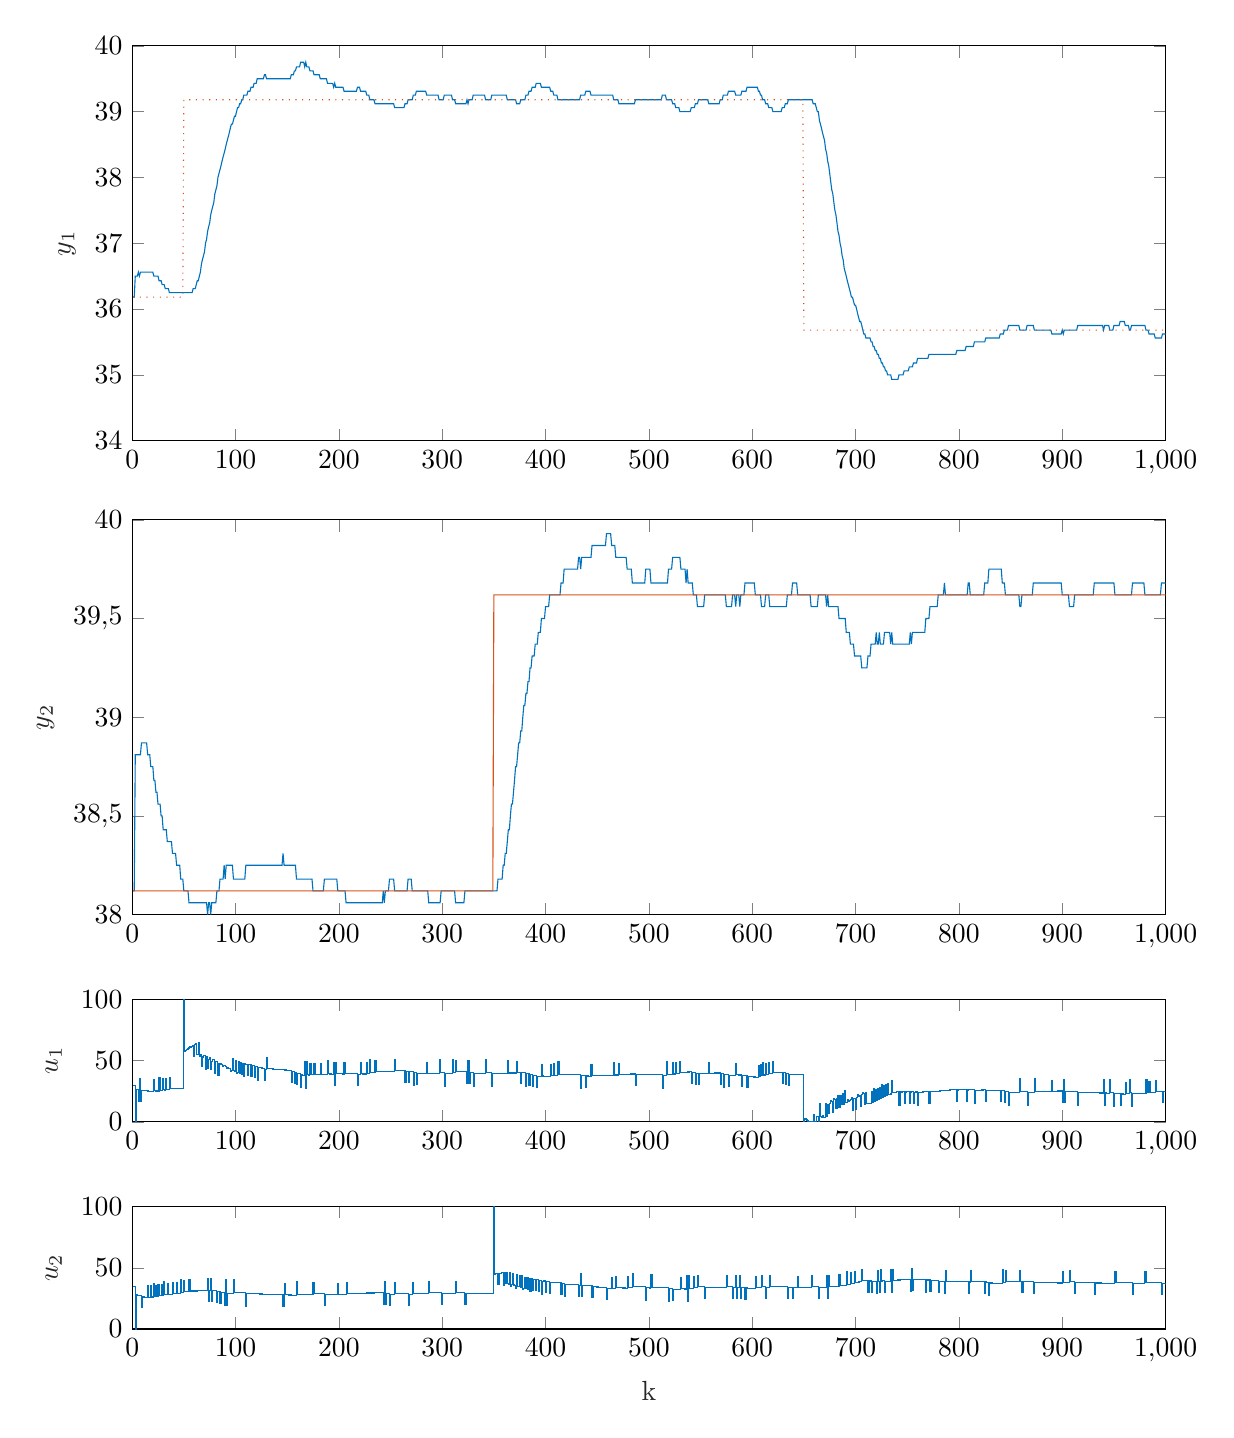
\begin{tikzpicture}

\begin{axis}[%
width=5.167in,
height=0.612in,
at={(0.646in,0.494in)},
scale only axis,
xmin=0,
xmax=1000,
xtick={0,100,200,300,400,500,600,700,800,900,1000},
xlabel style={font=\color{white!15!black}},
xlabel={k},
ymin=0,
ymax=100,
ytick={0,50,100},
ylabel style={font=\color{white!15!black}},
ylabel={$\text{u}_\text{2}$},
axis background/.style={fill=white}
]
\addplot[const plot, color=mycolor1, forget plot] table[row sep=crcr] {%
1	35\\
2	35\\
3	0\\
4	27.87\\
5	27.7167\\
6	27.5633\\
7	27.41\\
8	27.2567\\
9	17.497\\
10	26.33\\
11	26.1633\\
12	25.9967\\
13	25.83\\
14	25.6633\\
15	35.10333\\
16	25.95\\
17	25.7967\\
18	35.25\\
19	26.11\\
20	25.97\\
21	37.0378\\
22	26.4133\\
23	35.89556\\
24	26.7844\\
25	36.28\\
26	27.1822\\
27	27.0844\\
28	36.5933\\
29	27.5089\\
30	38.6322\\
31	28.0633\\
32	27.9944\\
33	27.9256\\
34	37.4633\\
35	28.4078\\
36	28.3522\\
37	28.2967\\
38	28.2411\\
39	37.7922\\
40	28.75\\
41	28.7078\\
42	28.6656\\
43	38.23\\
44	29.2011\\
45	29.1722\\
46	29.1433\\
47	40.3222\\
48	29.8089\\
49	29.7956\\
50	39.3889\\
51	30.3889\\
52	30.3889\\
53	30.3889\\
54	30.3889\\
55	39.9956\\
56	31.0089\\
57	31.0222\\
58	31.0356\\
59	31.0489\\
60	31.0622\\
61	31.0756\\
62	31.0889\\
63	31.1022\\
64	31.1156\\
65	31.1289\\
66	31.1422\\
67	31.1556\\
68	31.1689\\
69	31.1822\\
70	31.1956\\
71	31.2089\\
72	31.2222\\
73	40.8422\\
74	22.262\\
75	31.2756\\
76	40.8956\\
77	22.316\\
78	31.3289\\
79	31.3422\\
80	31.3556\\
81	31.3689\\
82	21.776\\
83	30.7756\\
84	30.7756\\
85	21.169\\
86	30.1556\\
87	30.1422\\
88	30.1289\\
89	18.908\\
90	40.5867\\
91	18.866\\
92	29.3367\\
93	29.3078\\
94	29.2789\\
95	29.25\\
96	29.2211\\
97	29.1922\\
98	40.3711\\
99	29.8578\\
100	29.8444\\
101	29.8311\\
102	29.8178\\
103	29.8044\\
104	29.7911\\
105	29.7778\\
106	29.7644\\
107	29.7511\\
108	29.7378\\
109	29.7244\\
110	18.503\\
111	28.9744\\
112	28.9456\\
113	28.9167\\
114	28.8878\\
115	28.8589\\
116	28.83\\
117	28.8011\\
118	28.7722\\
119	28.7433\\
120	28.7144\\
121	28.6856\\
122	28.6567\\
123	28.6278\\
124	28.5989\\
125	28.57\\
126	28.5411\\
127	28.5122\\
128	28.4833\\
129	28.4544\\
130	28.4256\\
131	28.3967\\
132	28.3678\\
133	28.3389\\
134	28.31\\
135	28.2811\\
136	28.2522\\
137	28.2233\\
138	28.1944\\
139	28.1656\\
140	28.1367\\
141	28.1078\\
142	28.0789\\
143	28.05\\
144	28.0211\\
145	27.9922\\
146	18.357\\
147	36.9211\\
148	27.8922\\
149	27.8633\\
150	27.8344\\
151	27.8056\\
152	27.7767\\
153	27.7478\\
154	27.7189\\
155	27.69\\
156	27.6611\\
157	27.6322\\
158	27.6033\\
159	38.7822\\
160	28.2689\\
161	28.2556\\
162	28.2422\\
163	28.2289\\
164	28.2156\\
165	28.2022\\
166	28.1889\\
167	28.1756\\
168	28.1622\\
169	28.1489\\
170	28.1356\\
171	28.1222\\
172	28.1089\\
173	28.0956\\
174	28.0822\\
175	37.6756\\
176	28.6756\\
177	28.6756\\
178	28.6756\\
179	28.6756\\
180	28.6756\\
181	28.6756\\
182	28.6756\\
183	28.6756\\
184	28.6756\\
185	28.6756\\
186	19.069\\
187	28.0556\\
188	28.0422\\
189	28.0289\\
190	28.0156\\
191	28.0022\\
192	27.9889\\
193	27.9756\\
194	27.9622\\
195	27.9489\\
196	27.9356\\
197	27.9222\\
198	27.9089\\
199	37.5022\\
200	28.5022\\
201	28.5022\\
202	28.5022\\
203	28.5022\\
204	28.5022\\
205	28.5022\\
206	28.5022\\
207	38.1089\\
208	29.1222\\
209	29.1356\\
210	29.1489\\
211	29.1622\\
212	29.1756\\
213	29.1889\\
214	29.2022\\
215	29.2156\\
216	29.2289\\
217	29.2422\\
218	29.2556\\
219	29.2689\\
220	29.2822\\
221	29.2956\\
222	29.3089\\
223	29.3222\\
224	29.3356\\
225	29.3489\\
226	29.3622\\
227	29.3756\\
228	29.3889\\
229	29.4022\\
230	29.4156\\
231	29.4289\\
232	29.4422\\
233	29.4556\\
234	29.4689\\
235	29.4822\\
236	29.4956\\
237	29.5089\\
238	29.5222\\
239	29.5356\\
240	29.5489\\
241	29.5622\\
242	29.5756\\
243	19.982\\
244	38.5889\\
245	19.996\\
246	28.9956\\
247	28.9956\\
248	28.9956\\
249	19.389\\
250	28.3756\\
251	28.3622\\
252	28.3489\\
253	28.3356\\
254	37.9289\\
255	28.9289\\
256	28.9289\\
257	28.9289\\
258	28.9289\\
259	28.9289\\
260	28.9289\\
261	28.9289\\
262	28.9289\\
263	28.9289\\
264	28.9289\\
265	28.9289\\
266	28.9289\\
267	19.322\\
268	28.3089\\
269	28.2956\\
270	28.2822\\
271	37.8756\\
272	28.8756\\
273	28.8756\\
274	28.8756\\
275	28.8756\\
276	28.8756\\
277	28.8756\\
278	28.8756\\
279	28.8756\\
280	28.8756\\
281	28.8756\\
282	28.8756\\
283	28.8756\\
284	28.8756\\
285	28.8756\\
286	28.8756\\
287	38.4822\\
288	29.4956\\
289	29.5089\\
290	29.5222\\
291	29.5356\\
292	29.5489\\
293	29.5622\\
294	29.5756\\
295	29.5889\\
296	29.6022\\
297	29.6156\\
298	29.6289\\
299	20.036\\
300	29.0356\\
301	29.0356\\
302	29.0356\\
303	29.0356\\
304	29.0356\\
305	29.0356\\
306	29.0356\\
307	29.0356\\
308	29.0356\\
309	29.0356\\
310	29.0356\\
311	29.0356\\
312	29.0356\\
313	38.6422\\
314	29.6556\\
315	29.6689\\
316	29.6822\\
317	29.6956\\
318	29.7089\\
319	29.7222\\
320	29.7356\\
321	29.7489\\
322	20.156\\
323	29.1556\\
324	29.1556\\
325	29.1556\\
326	29.1556\\
327	29.1556\\
328	29.1556\\
329	29.1556\\
330	29.1556\\
331	29.1556\\
332	29.1556\\
333	29.1556\\
334	29.1556\\
335	29.1556\\
336	29.1556\\
337	29.1556\\
338	29.1556\\
339	29.1556\\
340	29.1556\\
341	29.1556\\
342	29.1556\\
343	29.1556\\
344	29.1556\\
345	29.1556\\
346	29.1556\\
347	29.1556\\
348	29.1556\\
349	29.1556\\
350	100\\
351	44.6556\\
352	44.9889\\
353	45.322\\
354	36.0489\\
355	45.369\\
356	45.689\\
357	46.009\\
358	46.329\\
359	35.44111\\
360	46.246\\
361	36.9433\\
362	46.234\\
363	36.9189\\
364	36.59\\
365	45.854\\
366	34.911111\\
367	36.0533\\
368	45.289\\
369	35.91778\\
370	35.53333\\
371	33.5344\\
372	44.2278\\
373	34.81444\\
374	34.38778\\
375	43.5544\\
376	34.11444\\
377	43.2678\\
378	32.2133\\
379	33.2444\\
380	42.3689\\
381	32.8867\\
382	41.9978\\
383	32.5022\\
384	41.6\\
385	30.49\\
386	41.0722\\
387	31.5478\\
388	40.6167\\
389	40.6856\\
390	31.1478\\
391	40.2033\\
392	40.2589\\
393	30.7078\\
394	39.75\\
395	39.7922\\
396	28.6267\\
397	39.1533\\
398	39.18\\
399	39.2067\\
400	29.6267\\
401	38.64\\
402	38.6533\\
403	38.6667\\
404	29.0733\\
405	38.0733\\
406	38.0733\\
407	38.0733\\
408	38.0733\\
409	38.0733\\
410	38.0733\\
411	38.0733\\
412	38.0733\\
413	38.0733\\
414	38.0733\\
415	28.4667\\
416	37.4533\\
417	37.44\\
418	26.2189\\
419	36.69\\
420	36.6611\\
421	36.6322\\
422	36.6033\\
423	36.5744\\
424	36.5456\\
425	36.5167\\
426	36.4878\\
427	36.4589\\
428	36.43\\
429	36.4011\\
430	36.3722\\
431	36.3433\\
432	26.7078\\
433	35.66556\\
434	45.23\\
435	26.5944\\
436	35.55222\\
437	35.51\\
438	35.46778\\
439	35.42556\\
440	35.38333\\
441	35.34111\\
442	35.29889\\
443	35.25667\\
444	35.21444\\
445	25.5656\\
446	34.51\\
447	34.45444\\
448	34.39889\\
449	34.34333\\
450	34.28778\\
451	34.23222\\
452	34.17667\\
453	34.12111\\
454	34.06556\\
455	34.01\\
456	33.9544\\
457	33.8989\\
458	33.8433\\
459	24.181\\
460	33.1122\\
461	33.0433\\
462	32.9744\\
463	32.9056\\
464	42.4433\\
465	33.3878\\
466	33.3322\\
467	33.2767\\
468	42.8278\\
469	33.7856\\
470	33.7433\\
471	33.7011\\
472	33.6589\\
473	33.6167\\
474	33.5744\\
475	33.5322\\
476	33.49\\
477	33.4478\\
478	33.4056\\
479	42.97\\
480	33.9411\\
481	33.9122\\
482	33.8833\\
483	33.8544\\
484	45.033\\
485	34.52\\
486	34.50667\\
487	34.49333\\
488	34.48\\
489	34.46667\\
490	34.45333\\
491	34.44\\
492	34.42667\\
493	34.41333\\
494	34.4\\
495	34.38667\\
496	34.37333\\
497	23.152\\
498	33.6233\\
499	33.5944\\
500	33.5656\\
501	33.5367\\
502	44.7156\\
503	34.20222\\
504	34.18889\\
505	34.17556\\
506	34.16222\\
507	34.14889\\
508	34.13556\\
509	34.12222\\
510	34.10889\\
511	34.09556\\
512	34.08222\\
513	34.06889\\
514	34.05556\\
515	34.04222\\
516	34.02889\\
517	34.01556\\
518	34.00222\\
519	22.781\\
520	33.2522\\
521	33.2233\\
522	33.1944\\
523	23.559\\
524	32.5167\\
525	32.4744\\
526	32.4322\\
527	32.39\\
528	32.3478\\
529	32.3056\\
530	32.2633\\
531	41.8278\\
532	32.7989\\
533	32.77\\
534	32.7411\\
535	32.7122\\
536	43.8911\\
537	22.17\\
538	43.8489\\
539	33.3356\\
540	33.3222\\
541	33.3089\\
542	33.2956\\
543	42.8889\\
544	33.8889\\
545	33.8889\\
546	33.8889\\
547	43.4956\\
548	34.50889\\
549	34.52222\\
550	34.53556\\
551	34.54889\\
552	34.56222\\
553	34.57556\\
554	24.982\\
555	33.9822\\
556	33.9822\\
557	33.9822\\
558	33.9822\\
559	33.9822\\
560	33.9822\\
561	33.9822\\
562	33.9822\\
563	33.9822\\
564	33.9822\\
565	33.9822\\
566	33.9822\\
567	33.9822\\
568	33.9822\\
569	33.9822\\
570	33.9822\\
571	33.9822\\
572	33.9822\\
573	33.9822\\
574	33.9822\\
575	43.5889\\
576	34.60222\\
577	34.61556\\
578	34.62889\\
579	34.64222\\
580	34.65556\\
581	25.0622\\
582	34.06222\\
583	34.06222\\
584	43.6689\\
585	25.0756\\
586	34.07556\\
587	34.07556\\
588	43.6822\\
589	25.0889\\
590	34.08889\\
591	34.08889\\
592	34.08889\\
593	24.482\\
594	33.4689\\
595	33.4556\\
596	33.4422\\
597	33.4289\\
598	33.4156\\
599	33.4022\\
600	33.3889\\
601	33.3756\\
602	33.3622\\
603	42.9556\\
604	33.9556\\
605	33.9556\\
606	33.9556\\
607	33.9556\\
608	33.9556\\
609	43.5622\\
610	34.57556\\
611	34.58889\\
612	34.60222\\
613	25.0089\\
614	34.00889\\
615	34.00889\\
616	34.00889\\
617	43.6156\\
618	34.62889\\
619	34.64222\\
620	34.65556\\
621	34.66889\\
622	34.68222\\
623	34.69556\\
624	34.70889\\
625	34.72222\\
626	34.73556\\
627	34.74889\\
628	34.76222\\
629	34.77556\\
630	34.78889\\
631	34.80222\\
632	34.81556\\
633	34.82889\\
634	25.2356\\
635	34.23556\\
636	34.23556\\
637	34.23556\\
638	34.23556\\
639	24.629\\
640	33.6156\\
641	33.6022\\
642	33.5889\\
643	33.5756\\
644	43.1689\\
645	34.16889\\
646	34.16889\\
647	34.16889\\
648	34.16889\\
649	34.16889\\
650	34.16889\\
651	34.16889\\
652	34.16889\\
653	34.16889\\
654	34.16889\\
655	34.16889\\
656	34.16889\\
657	43.7756\\
658	34.78889\\
659	34.80222\\
660	34.81556\\
661	34.82889\\
662	34.84222\\
663	34.85556\\
664	25.2622\\
665	34.26222\\
666	34.26222\\
667	34.26222\\
668	34.26222\\
669	34.26222\\
670	34.26222\\
671	34.26222\\
672	43.8689\\
673	25.2756\\
674	43.8822\\
675	34.89556\\
676	34.908889\\
677	34.922222\\
678	34.935556\\
679	34.948889\\
680	34.962222\\
681	34.975556\\
682	34.988889\\
683	35.0022222\\
684	44.6222\\
685	35.64889\\
686	35.67556\\
687	35.70222\\
688	35.72889\\
689	35.75556\\
690	35.78222\\
691	47.017\\
692	36.5589\\
693	36.6011\\
694	36.6433\\
695	46.292\\
696	37.3478\\
697	37.4033\\
698	37.4589\\
699	47.121\\
700	38.19\\
701	38.2589\\
702	38.3278\\
703	38.3967\\
704	38.4656\\
705	38.5344\\
706	48.21\\
707	39.2922\\
708	39.3744\\
709	39.4567\\
710	39.5389\\
711	39.6211\\
712	30.0967\\
713	39.1656\\
714	39.2344\\
715	29.6967\\
716	38.7522\\
717	38.8078\\
718	38.8633\\
719	38.9189\\
720	29.3678\\
721	48.017\\
722	39.0722\\
723	29.5211\\
724	48.17\\
725	39.2256\\
726	39.2811\\
727	39.3367\\
728	29.7856\\
729	38.8278\\
730	38.87\\
731	38.9122\\
732	38.9544\\
733	38.9967\\
734	48.646\\
735	30.0944\\
736	48.743\\
737	39.7989\\
738	39.8544\\
739	39.91\\
740	39.9656\\
741	40.0211\\
742	40.0767\\
743	40.1322\\
744	40.1878\\
745	40.2433\\
746	40.2989\\
747	40.3544\\
748	40.41\\
749	40.4656\\
750	40.5211\\
751	40.5767\\
752	40.6322\\
753	31.0811\\
754	49.73\\
755	31.1789\\
756	40.2211\\
757	40.2633\\
758	40.3056\\
759	40.3478\\
760	40.39\\
761	40.4322\\
762	40.4744\\
763	40.5167\\
764	40.5589\\
765	40.6011\\
766	40.6433\\
767	40.6856\\
768	29.52\\
769	40.0467\\
770	40.0733\\
771	40.1\\
772	30.52\\
773	39.5333\\
774	39.5467\\
775	39.56\\
776	39.5733\\
777	39.5867\\
778	39.6\\
779	39.6133\\
780	30.02\\
781	39.02\\
782	39.02\\
783	39.02\\
784	39.02\\
785	39.02\\
786	29.4133\\
787	48.007\\
788	39.0067\\
789	39.0067\\
790	39.0067\\
791	39.0067\\
792	39.0067\\
793	39.0067\\
794	39.0067\\
795	39.0067\\
796	39.0067\\
797	39.0067\\
798	39.0067\\
799	39.0067\\
800	39.0067\\
801	39.0067\\
802	39.0067\\
803	39.0067\\
804	39.0067\\
805	39.0067\\
806	39.0067\\
807	39.0067\\
808	39.0067\\
809	29.4\\
810	38.3867\\
811	47.98\\
812	38.98\\
813	38.98\\
814	38.98\\
815	38.98\\
816	38.98\\
817	38.98\\
818	38.98\\
819	38.98\\
820	38.98\\
821	38.98\\
822	38.98\\
823	38.98\\
824	38.98\\
825	29.3733\\
826	38.36\\
827	38.3467\\
828	38.3333\\
829	27.1122\\
830	37.5833\\
831	37.5544\\
832	37.5256\\
833	37.4967\\
834	37.4678\\
835	37.4389\\
836	37.41\\
837	37.3811\\
838	37.3522\\
839	37.3233\\
840	37.2944\\
841	37.2656\\
842	48.444\\
843	37.9311\\
844	37.9178\\
845	47.511\\
846	38.5111\\
847	38.5111\\
848	38.5111\\
849	38.5111\\
850	38.5111\\
851	38.5111\\
852	38.5111\\
853	38.5111\\
854	38.5111\\
855	38.5111\\
856	38.5111\\
857	38.5111\\
858	38.5111\\
859	48.118\\
860	39.1311\\
861	29.5378\\
862	38.5378\\
863	38.5378\\
864	38.5378\\
865	38.5378\\
866	38.5378\\
867	38.5378\\
868	38.5378\\
869	38.5378\\
870	38.5378\\
871	38.5378\\
872	28.9311\\
873	37.9178\\
874	37.9044\\
875	37.8911\\
876	37.8778\\
877	37.8644\\
878	37.8511\\
879	37.8378\\
880	37.8244\\
881	37.8111\\
882	37.7978\\
883	37.7844\\
884	37.7711\\
885	37.7578\\
886	37.7444\\
887	37.7311\\
888	37.7178\\
889	37.7044\\
890	37.6911\\
891	37.6778\\
892	37.6644\\
893	37.6511\\
894	37.6378\\
895	37.6244\\
896	37.6111\\
897	37.5978\\
898	37.5844\\
899	37.5711\\
900	47.164\\
901	38.1644\\
902	38.1644\\
903	38.1644\\
904	38.1644\\
905	38.1644\\
906	38.1644\\
907	47.771\\
908	38.7844\\
909	38.7978\\
910	38.8111\\
911	38.8244\\
912	29.2311\\
913	38.2311\\
914	38.2311\\
915	38.2311\\
916	38.2311\\
917	38.2311\\
918	38.2311\\
919	38.2311\\
920	38.2311\\
921	38.2311\\
922	38.2311\\
923	38.2311\\
924	38.2311\\
925	38.2311\\
926	38.2311\\
927	38.2311\\
928	38.2311\\
929	38.2311\\
930	38.2311\\
931	28.6244\\
932	37.6111\\
933	37.5978\\
934	37.5844\\
935	37.5711\\
936	37.5578\\
937	37.5444\\
938	37.5311\\
939	37.5178\\
940	37.5044\\
941	37.4911\\
942	37.4778\\
943	37.4644\\
944	37.4511\\
945	37.4378\\
946	37.4244\\
947	37.4111\\
948	37.3978\\
949	37.3844\\
950	37.3711\\
951	46.964\\
952	37.9644\\
953	37.9644\\
954	37.9644\\
955	37.9644\\
956	37.9644\\
957	37.9644\\
958	37.9644\\
959	37.9644\\
960	37.9644\\
961	37.9644\\
962	37.9644\\
963	37.9644\\
964	37.9644\\
965	37.9644\\
966	37.9644\\
967	37.9644\\
968	28.3578\\
969	37.3444\\
970	37.3311\\
971	37.3178\\
972	37.3044\\
973	37.2911\\
974	37.2778\\
975	37.2644\\
976	37.2511\\
977	37.2378\\
978	37.2244\\
979	37.2111\\
980	46.804\\
981	37.8044\\
982	37.8044\\
983	37.8044\\
984	37.8044\\
985	37.8044\\
986	37.8044\\
987	37.8044\\
988	37.8044\\
989	37.8044\\
990	37.8044\\
991	37.8044\\
992	37.8044\\
993	37.8044\\
994	37.8044\\
995	37.8044\\
996	28.1978\\
997	37.1844\\
998	37.1711\\
999	37.1578\\
1000	37.1444\\
};
\end{axis}

\begin{axis}[%
width=5.167in,
height=0.612in,
at={(0.646in,1.53in)},
scale only axis,
xmin=0,
xmax=1000,
xtick={0,100,200,300,400,500,600,700,800,900,1000},
ymin=0,
ymax=100,
ytick={0,50,100},
ylabel style={font=\color{white!15!black}},
ylabel={$\text{u}_\text{1}$},
axis background/.style={fill=white}
]
\addplot[const plot, color=mycolor1, forget plot] table[row sep=crcr] {%
1	30\\
2	30\\
3	0\\
4	26.6933\\
5	26.6222\\
6	16.944\\
7	35.4667\\
8	16.789\\
9	25.7044\\
10	25.62\\
11	25.5356\\
12	25.4511\\
13	25.3667\\
14	25.2822\\
15	25.1978\\
16	25.1133\\
17	25.0289\\
18	24.9444\\
19	24.86\\
20	24.7756\\
21	34.2978\\
22	25.2267\\
23	25.1556\\
24	25.0844\\
25	25.0133\\
26	36.15\\
27	25.5944\\
28	25.5389\\
29	35.09\\
30	26.0478\\
31	26.0056\\
32	35.57\\
33	26.5411\\
34	26.5122\\
35	26.4833\\
36	36.0611\\
37	27.0456\\
38	27.03\\
39	27.0144\\
40	26.9989\\
41	26.9833\\
42	26.9678\\
43	26.9522\\
44	26.9367\\
45	26.9211\\
46	26.9056\\
47	26.89\\
48	26.8744\\
49	26.8589\\
50	100\\
51	57.828\\
52	58.479\\
53	59.13\\
54	59.781\\
55	60.432\\
56	61.083\\
57	61.734\\
58	62.386\\
59	53.43\\
60	63.068\\
61	63.706\\
62	54.737\\
63	54.754\\
64	64.366\\
65	53.769\\
66	55.258\\
67	45.627\\
68	52.974\\
69	54.408\\
70	54.328\\
71	43.027\\
72	53.404\\
73	43.662\\
74	50.899\\
75	52.221\\
76	42.423\\
77	49.604\\
78	50.871\\
79	50.624\\
80	39.1567\\
81	49.368\\
82	49.066\\
83	37.5422\\
84	47.698\\
85	47.34\\
86	46.969\\
87	44.983\\
88	46.083\\
89	45.67\\
90	45.243\\
91	43.202\\
92	44.247\\
93	43.778\\
94	43.296\\
95	41.199\\
96	42.188\\
97	51.27\\
98	41.746\\
99	41.208\\
100	50.263\\
101	39.1111\\
102	40.044\\
103	49.071\\
104	39.4911\\
105	48.504\\
106	38.9111\\
107	47.911\\
108	36.7033\\
109	47.188\\
110	47.172\\
111	47.157\\
112	37.5344\\
113	46.506\\
114	46.477\\
115	36.8411\\
116	45.799\\
117	45.757\\
118	36.1078\\
119	45.052\\
120	44.997\\
121	33.7333\\
122	44.162\\
123	44.091\\
124	44.02\\
125	43.949\\
126	43.878\\
127	43.807\\
128	34.1289\\
129	43.044\\
130	52.567\\
131	43.496\\
132	43.424\\
133	43.353\\
134	43.282\\
135	43.211\\
136	43.14\\
137	43.069\\
138	42.998\\
139	42.927\\
140	42.856\\
141	42.784\\
142	42.713\\
143	42.642\\
144	42.571\\
145	42.5\\
146	42.429\\
147	42.358\\
148	42.287\\
149	42.216\\
150	42.144\\
151	42.073\\
152	42.002\\
153	41.931\\
154	32.2533\\
155	41.169\\
156	41.084\\
157	31.3933\\
158	40.296\\
159	30.59111\\
160	39.48\\
161	39.3689\\
162	39.2578\\
163	27.9389\\
164	38.3122\\
165	38.1856\\
166	38.0589\\
167	49.14\\
168	27.3211\\
169	48.902\\
170	38.2911\\
171	38.18\\
172	47.676\\
173	38.5778\\
174	38.48\\
175	38.3822\\
176	47.891\\
177	38.8067\\
178	38.7222\\
179	38.6378\\
180	38.5533\\
181	38.4689\\
182	47.991\\
183	38.92\\
184	38.8489\\
185	38.7778\\
186	38.7067\\
187	38.6356\\
188	38.5644\\
189	49.701\\
190	39.1456\\
191	39.09\\
192	39.0344\\
193	38.9789\\
194	38.9233\\
195	48.474\\
196	29.82556\\
197	48.377\\
198	39.3344\\
199	39.2922\\
200	39.25\\
201	39.2078\\
202	39.1656\\
203	39.1233\\
204	39.0811\\
205	48.646\\
206	39.6167\\
207	39.5878\\
208	39.5589\\
209	39.53\\
210	39.5011\\
211	39.4722\\
212	39.4433\\
213	39.4144\\
214	39.3856\\
215	39.3567\\
216	39.3278\\
217	39.2989\\
218	29.66333\\
219	38.6211\\
220	38.5789\\
221	48.143\\
222	39.1144\\
223	39.0856\\
224	39.0567\\
225	39.0278\\
226	38.9989\\
227	48.577\\
228	39.5611\\
229	39.5456\\
230	50.738\\
231	40.238\\
232	40.238\\
233	40.238\\
234	40.238\\
235	49.844\\
236	40.858\\
237	40.871\\
238	40.884\\
239	40.898\\
240	40.911\\
241	40.924\\
242	40.938\\
243	40.951\\
244	40.964\\
245	40.978\\
246	40.991\\
247	41.004\\
248	41.018\\
249	41.031\\
250	41.044\\
251	41.058\\
252	41.071\\
253	41.084\\
254	50.704\\
255	41.731\\
256	41.758\\
257	41.784\\
258	41.811\\
259	41.838\\
260	41.864\\
261	41.891\\
262	41.918\\
263	41.944\\
264	32.3644\\
265	41.378\\
266	41.391\\
267	31.7978\\
268	40.798\\
269	40.798\\
270	40.798\\
271	40.798\\
272	29.59\\
273	40.074\\
274	40.059\\
275	30.43667\\
276	39.4078\\
277	39.3789\\
278	39.35\\
279	39.3211\\
280	39.2922\\
281	39.2633\\
282	39.2344\\
283	39.2056\\
284	39.1767\\
285	48.754\\
286	39.7389\\
287	39.7233\\
288	39.7078\\
289	39.6922\\
290	39.6767\\
291	39.6611\\
292	39.6456\\
293	39.63\\
294	39.6144\\
295	39.5989\\
296	39.5833\\
297	50.776\\
298	40.276\\
299	40.276\\
300	40.276\\
301	40.276\\
302	29.06778\\
303	39.5522\\
304	39.5367\\
305	39.5211\\
306	39.5056\\
307	39.49\\
308	39.4744\\
309	39.4589\\
310	50.651\\
311	40.151\\
312	40.151\\
313	49.758\\
314	40.771\\
315	40.784\\
316	40.798\\
317	40.811\\
318	40.824\\
319	40.838\\
320	40.851\\
321	40.864\\
322	40.878\\
323	40.891\\
324	31.2978\\
325	49.904\\
326	31.3111\\
327	40.311\\
328	40.311\\
329	40.311\\
330	29.10333\\
331	39.5878\\
332	39.5722\\
333	39.5567\\
334	39.5411\\
335	39.5256\\
336	39.51\\
337	39.4944\\
338	39.4789\\
339	39.4633\\
340	39.4478\\
341	39.4322\\
342	50.624\\
343	40.124\\
344	40.124\\
345	40.124\\
346	40.124\\
347	40.124\\
348	28.9167\\
349	39.4011\\
350	39.3856\\
351	39.37\\
352	39.3544\\
353	39.3389\\
354	39.3233\\
355	39.3078\\
356	39.2922\\
357	39.2767\\
358	39.2611\\
359	39.2456\\
360	39.23\\
361	39.2144\\
362	39.1989\\
363	50.391\\
364	39.8911\\
365	39.8911\\
366	39.8911\\
367	39.8911\\
368	39.8911\\
369	39.8911\\
370	39.8911\\
371	39.8911\\
372	49.498\\
373	40.511\\
374	40.524\\
375	40.538\\
376	30.94444\\
377	39.9444\\
378	39.9444\\
379	39.9444\\
380	39.9444\\
381	28.7367\\
382	39.2211\\
383	39.2056\\
384	29.58333\\
385	38.5544\\
386	38.5256\\
387	28.89\\
388	37.8478\\
389	37.8056\\
390	37.7633\\
391	28.1144\\
392	37.0589\\
393	37.0033\\
394	36.9478\\
395	36.8922\\
396	46.443\\
397	37.4011\\
398	37.3589\\
399	37.3167\\
400	37.2744\\
401	37.2322\\
402	37.19\\
403	37.1478\\
404	37.1056\\
405	46.67\\
406	37.6411\\
407	37.6122\\
408	47.19\\
409	38.1744\\
410	38.1589\\
411	38.1433\\
412	49.336\\
413	38.8356\\
414	38.8356\\
415	38.8356\\
416	38.8356\\
417	38.8356\\
418	38.8356\\
419	38.8356\\
420	38.8356\\
421	38.8356\\
422	38.8356\\
423	38.8356\\
424	38.8356\\
425	38.8356\\
426	38.8356\\
427	38.8356\\
428	38.8356\\
429	38.8356\\
430	38.8356\\
431	38.8356\\
432	38.8356\\
433	38.8356\\
434	27.6278\\
435	38.1122\\
436	38.0967\\
437	38.0811\\
438	38.0656\\
439	28.4433\\
440	37.4144\\
441	37.3856\\
442	37.3567\\
443	37.3278\\
444	46.906\\
445	37.89\\
446	37.8744\\
447	37.8589\\
448	37.8433\\
449	37.8278\\
450	37.8122\\
451	37.7967\\
452	37.7811\\
453	37.7656\\
454	37.75\\
455	37.7344\\
456	37.7189\\
457	37.7033\\
458	37.6878\\
459	37.6722\\
460	37.6567\\
461	37.6411\\
462	37.6256\\
463	37.61\\
464	37.5944\\
465	37.5789\\
466	48.771\\
467	38.2711\\
468	38.2711\\
469	38.2711\\
470	38.2711\\
471	47.878\\
472	38.8911\\
473	38.9044\\
474	38.9178\\
475	38.9311\\
476	38.9444\\
477	38.9578\\
478	38.9711\\
479	38.9844\\
480	38.9978\\
481	39.0111\\
482	39.0244\\
483	39.0378\\
484	39.0511\\
485	39.0644\\
486	39.0778\\
487	29.48444\\
488	38.4844\\
489	38.4844\\
490	38.4844\\
491	38.4844\\
492	38.4844\\
493	38.4844\\
494	38.4844\\
495	38.4844\\
496	38.4844\\
497	38.4844\\
498	38.4844\\
499	38.4844\\
500	38.4844\\
501	38.4844\\
502	38.4844\\
503	38.4844\\
504	38.4844\\
505	38.4844\\
506	38.4844\\
507	38.4844\\
508	38.4844\\
509	38.4844\\
510	38.4844\\
511	38.4844\\
512	38.4844\\
513	27.2767\\
514	37.7611\\
515	37.7456\\
516	37.73\\
517	48.922\\
518	38.4222\\
519	38.4222\\
520	38.4222\\
521	38.4222\\
522	38.4222\\
523	48.029\\
524	39.0422\\
525	39.0556\\
526	48.676\\
527	39.7022\\
528	39.7289\\
529	39.7556\\
530	49.389\\
531	40.429\\
532	40.469\\
533	40.509\\
534	40.549\\
535	40.589\\
536	40.629\\
537	40.669\\
538	40.709\\
539	40.749\\
540	40.789\\
541	31.2222\\
542	40.249\\
543	40.276\\
544	40.302\\
545	30.72222\\
546	39.7356\\
547	39.7489\\
548	30.15556\\
549	39.1556\\
550	39.1556\\
551	39.1556\\
552	39.1556\\
553	39.1556\\
554	39.1556\\
555	39.1556\\
556	39.1556\\
557	39.1556\\
558	48.762\\
559	39.7756\\
560	39.7889\\
561	39.8022\\
562	39.8156\\
563	39.8289\\
564	39.8422\\
565	39.8556\\
566	39.8689\\
567	39.8822\\
568	39.8956\\
569	30.30222\\
570	39.3022\\
571	39.3022\\
572	28.0944\\
573	38.5789\\
574	38.5633\\
575	38.5478\\
576	38.5322\\
577	28.91\\
578	37.8811\\
579	37.8522\\
580	37.8233\\
581	37.7944\\
582	37.7656\\
583	37.7367\\
584	47.314\\
585	38.2989\\
586	38.2833\\
587	38.2678\\
588	38.2522\\
589	38.2367\\
590	28.6144\\
591	37.5856\\
592	37.5567\\
593	37.5278\\
594	37.4989\\
595	27.8633\\
596	36.8211\\
597	36.7789\\
598	36.7367\\
599	36.6944\\
600	36.6522\\
601	36.61\\
602	36.5678\\
603	36.5256\\
604	36.4833\\
605	36.4411\\
606	46.006\\
607	36.9767\\
608	46.554\\
609	37.5389\\
610	48.731\\
611	38.2311\\
612	38.2311\\
613	47.838\\
614	38.8511\\
615	38.8644\\
616	48.484\\
617	39.5111\\
618	39.5378\\
619	39.5644\\
620	49.198\\
621	40.238\\
622	40.278\\
623	40.318\\
624	40.358\\
625	40.398\\
626	40.438\\
627	40.478\\
628	40.518\\
629	30.95111\\
630	39.9778\\
631	40.004\\
632	30.42444\\
633	39.4378\\
634	39.4511\\
635	29.85778\\
636	38.8578\\
637	38.8578\\
638	38.8578\\
639	38.8578\\
640	38.8578\\
641	38.8578\\
642	38.8578\\
643	38.8578\\
644	38.8578\\
645	38.8578\\
646	38.8578\\
647	38.8578\\
648	38.8578\\
649	38.8578\\
650	0\\
651	2.691\\
652	1.913\\
653	1.136\\
654	0.358000000000001\\
655	0\\
656	0\\
657	0\\
658	0\\
659	6.076\\
660	0\\
661	0\\
662	4.389\\
663	4.244\\
664	0\\
665	14.583\\
666	3.981\\
667	3.892\\
668	5.418\\
669	3.858\\
670	3.811\\
671	14.986\\
672	4.481\\
673	14.097\\
674	6.733\\
675	14.891\\
676	17.177\\
677	16.39\\
678	7.523\\
679	18.878\\
680	18.16\\
681	10.963\\
682	19.288\\
683	21.74\\
684	11.513\\
685	21.4067\\
686	14.321\\
687	22.7567\\
688	14.112\\
689	25.6889\\
690	15.587\\
691	15.998\\
692	18.023\\
693	16.963\\
694	17.417\\
695	17.883\\
696	19.964\\
697	9.353\\
698	18.849\\
699	19.358\\
700	10.273\\
701	19.796\\
702	21.9322\\
703	20.9833\\
704	21.5478\\
705	12.519\\
706	22.0967\\
707	24.2889\\
708	23.3956\\
709	14.409\\
710	24.0289\\
711	15.056\\
712	15.082\\
713	15.109\\
714	15.136\\
715	24.7689\\
716	15.809\\
717	27.0567\\
718	16.612\\
719	26.2744\\
720	17.343\\
721	27.0189\\
722	18.101\\
723	27.79\\
724	18.886\\
725	30.18889\\
726	19.8\\
727	29.51778\\
728	20.6422\\
729	30.37333\\
730	21.5111\\
731	31.2556\\
732	22.4067\\
733	22.5578\\
734	22.7089\\
735	34.0678\\
736	23.7344\\
737	23.9011\\
738	24.0678\\
739	24.2344\\
740	24.4011\\
741	24.5678\\
742	13.527\\
743	24.1778\\
744	24.3289\\
745	24.48\\
746	24.6311\\
747	15.176\\
748	24.3133\\
749	24.4511\\
750	24.5889\\
751	24.7267\\
752	15.258\\
753	24.3822\\
754	24.5067\\
755	24.6311\\
756	15.149\\
757	24.26\\
758	24.3711\\
759	24.4822\\
760	13.386\\
761	23.9811\\
762	24.0767\\
763	24.1722\\
764	24.2678\\
765	24.3633\\
766	24.4589\\
767	24.5544\\
768	24.65\\
769	24.7456\\
770	24.8411\\
771	15.33\\
772	24.4122\\
773	24.4944\\
774	24.5767\\
775	24.6589\\
776	24.7411\\
777	24.8233\\
778	24.9056\\
779	24.9878\\
780	25.07\\
781	25.1522\\
782	25.2344\\
783	25.3167\\
784	25.3989\\
785	25.4811\\
786	25.5633\\
787	25.6456\\
788	25.7278\\
789	25.81\\
790	25.8922\\
791	25.9744\\
792	26.0567\\
793	26.1389\\
794	26.2211\\
795	26.3033\\
796	26.3856\\
797	26.4678\\
798	16.943\\
799	26.0122\\
800	26.0811\\
801	26.15\\
802	26.2189\\
803	26.2878\\
804	26.3567\\
805	26.4256\\
806	26.4944\\
807	16.957\\
808	26.0122\\
809	26.0678\\
810	26.1233\\
811	26.1789\\
812	26.2344\\
813	26.29\\
814	26.3456\\
815	15.193\\
816	25.7333\\
817	25.7733\\
818	25.8133\\
819	25.8533\\
820	25.8933\\
821	25.9333\\
822	25.9733\\
823	26.0133\\
824	26.0533\\
825	26.0933\\
826	16.527\\
827	25.5533\\
828	25.58\\
829	25.6067\\
830	25.6333\\
831	25.66\\
832	25.6867\\
833	25.7133\\
834	25.74\\
835	25.7667\\
836	25.7933\\
837	25.82\\
838	25.8467\\
839	25.8733\\
840	16.293\\
841	25.3067\\
842	25.32\\
843	25.3333\\
844	15.74\\
845	24.74\\
846	24.74\\
847	24.74\\
848	13.532\\
849	24.0167\\
850	24.0011\\
851	23.9856\\
852	23.97\\
853	23.9544\\
854	23.9389\\
855	23.9233\\
856	23.9078\\
857	23.8922\\
858	23.8767\\
859	35.0689\\
860	24.5689\\
861	24.5689\\
862	24.5689\\
863	24.5689\\
864	24.5689\\
865	24.5689\\
866	13.361\\
867	23.8456\\
868	23.83\\
869	23.8144\\
870	23.7989\\
871	23.7833\\
872	23.7678\\
873	34.96\\
874	24.46\\
875	24.46\\
876	24.46\\
877	24.46\\
878	24.46\\
879	24.46\\
880	24.46\\
881	24.46\\
882	24.46\\
883	24.46\\
884	24.46\\
885	24.46\\
886	24.46\\
887	24.46\\
888	24.46\\
889	24.46\\
890	34.0667\\
891	25.08\\
892	25.0933\\
893	25.1067\\
894	25.12\\
895	25.1333\\
896	25.1467\\
897	25.16\\
898	25.1733\\
899	25.1867\\
900	15.593\\
901	34.2\\
902	15.607\\
903	24.6067\\
904	24.6067\\
905	24.6067\\
906	24.6067\\
907	24.6067\\
908	24.6067\\
909	24.6067\\
910	24.6067\\
911	24.6067\\
912	24.6067\\
913	24.6067\\
914	24.6067\\
915	13.399\\
916	23.8833\\
917	23.8678\\
918	23.8522\\
919	23.8367\\
920	23.8211\\
921	23.8056\\
922	23.79\\
923	23.7744\\
924	23.7589\\
925	23.7433\\
926	23.7278\\
927	23.7122\\
928	23.6967\\
929	23.6811\\
930	23.6656\\
931	23.65\\
932	23.6344\\
933	23.6189\\
934	23.6033\\
935	23.5878\\
936	23.5722\\
937	23.5567\\
938	23.5411\\
939	23.5256\\
940	34.7178\\
941	13.01\\
942	23.4944\\
943	23.4789\\
944	23.4633\\
945	23.4478\\
946	34.64\\
947	24.14\\
948	24.14\\
949	24.14\\
950	12.932\\
951	23.4167\\
952	23.4011\\
953	23.3856\\
954	23.37\\
955	23.3544\\
956	13.732\\
957	22.7033\\
958	22.6744\\
959	22.6456\\
960	22.6167\\
961	32.1944\\
962	23.1789\\
963	23.1633\\
964	23.1478\\
965	34.34\\
966	23.84\\
967	12.632\\
968	23.1167\\
969	23.1011\\
970	23.0856\\
971	23.07\\
972	23.0544\\
973	23.0389\\
974	23.0233\\
975	23.0078\\
976	22.9922\\
977	22.9767\\
978	22.9611\\
979	22.9456\\
980	22.93\\
981	34.1222\\
982	23.6222\\
983	23.6222\\
984	33.2289\\
985	24.2422\\
986	24.2556\\
987	24.2689\\
988	24.2822\\
989	24.2956\\
990	33.9156\\
991	24.9422\\
992	24.9689\\
993	24.9956\\
994	25.0222\\
995	25.0489\\
996	25.0756\\
997	15.496\\
998	24.5089\\
999	24.5222\\
1000	24.5356\\
};
\end{axis}

\begin{axis}[%
width=5.167in,
height=1.974in,
at={(0.646in,2.566in)},
scale only axis,
xmin=0,
xmax=1000,
xtick={0,100,200,300,400,500,600,700,800,900,1000},
ymin=38,
ymax=40,
ytick={38,38.5,39,39.5,40},
yticklabels={{38},{38,5},{39},{39,5},{40}},
ylabel style={font=\color{white!15!black}},
ylabel={$\text{y}_\text{2}$},
axis background/.style={fill=white}
]
\addplot [color=mycolor1, forget plot]
  table[row sep=crcr]{%
1	38.12\\
2	38.12\\
3	38.81\\
4	38.81\\
5	38.81\\
6	38.81\\
7	38.81\\
8	38.81\\
9	38.87\\
10	38.87\\
11	38.87\\
12	38.87\\
13	38.87\\
14	38.87\\
15	38.81\\
16	38.81\\
17	38.81\\
18	38.75\\
19	38.75\\
20	38.75\\
21	38.68\\
22	38.68\\
23	38.62\\
24	38.62\\
25	38.56\\
26	38.56\\
27	38.56\\
28	38.5\\
29	38.5\\
30	38.43\\
31	38.43\\
32	38.43\\
33	38.43\\
34	38.37\\
35	38.37\\
36	38.37\\
37	38.37\\
38	38.37\\
39	38.31\\
40	38.31\\
41	38.31\\
42	38.31\\
43	38.25\\
44	38.25\\
45	38.25\\
46	38.25\\
47	38.18\\
48	38.18\\
49	38.18\\
50	38.12\\
51	38.12\\
52	38.12\\
53	38.12\\
54	38.12\\
55	38.06\\
56	38.06\\
57	38.06\\
58	38.06\\
59	38.06\\
60	38.06\\
61	38.06\\
62	38.06\\
63	38.06\\
64	38.06\\
65	38.06\\
66	38.06\\
67	38.06\\
68	38.06\\
69	38.06\\
70	38.06\\
71	38.06\\
72	38.06\\
73	38\\
74	38.06\\
75	38.06\\
76	38\\
77	38.06\\
78	38.06\\
79	38.06\\
80	38.06\\
81	38.06\\
82	38.12\\
83	38.12\\
84	38.12\\
85	38.18\\
86	38.18\\
87	38.18\\
88	38.18\\
89	38.25\\
90	38.18\\
91	38.25\\
92	38.25\\
93	38.25\\
94	38.25\\
95	38.25\\
96	38.25\\
97	38.25\\
98	38.18\\
99	38.18\\
100	38.18\\
101	38.18\\
102	38.18\\
103	38.18\\
104	38.18\\
105	38.18\\
106	38.18\\
107	38.18\\
108	38.18\\
109	38.18\\
110	38.25\\
111	38.25\\
112	38.25\\
113	38.25\\
114	38.25\\
115	38.25\\
116	38.25\\
117	38.25\\
118	38.25\\
119	38.25\\
120	38.25\\
121	38.25\\
122	38.25\\
123	38.25\\
124	38.25\\
125	38.25\\
126	38.25\\
127	38.25\\
128	38.25\\
129	38.25\\
130	38.25\\
131	38.25\\
132	38.25\\
133	38.25\\
134	38.25\\
135	38.25\\
136	38.25\\
137	38.25\\
138	38.25\\
139	38.25\\
140	38.25\\
141	38.25\\
142	38.25\\
143	38.25\\
144	38.25\\
145	38.25\\
146	38.31\\
147	38.25\\
148	38.25\\
149	38.25\\
150	38.25\\
151	38.25\\
152	38.25\\
153	38.25\\
154	38.25\\
155	38.25\\
156	38.25\\
157	38.25\\
158	38.25\\
159	38.18\\
160	38.18\\
161	38.18\\
162	38.18\\
163	38.18\\
164	38.18\\
165	38.18\\
166	38.18\\
167	38.18\\
168	38.18\\
169	38.18\\
170	38.18\\
171	38.18\\
172	38.18\\
173	38.18\\
174	38.18\\
175	38.12\\
176	38.12\\
177	38.12\\
178	38.12\\
179	38.12\\
180	38.12\\
181	38.12\\
182	38.12\\
183	38.12\\
184	38.12\\
185	38.12\\
186	38.18\\
187	38.18\\
188	38.18\\
189	38.18\\
190	38.18\\
191	38.18\\
192	38.18\\
193	38.18\\
194	38.18\\
195	38.18\\
196	38.18\\
197	38.18\\
198	38.18\\
199	38.12\\
200	38.12\\
201	38.12\\
202	38.12\\
203	38.12\\
204	38.12\\
205	38.12\\
206	38.12\\
207	38.06\\
208	38.06\\
209	38.06\\
210	38.06\\
211	38.06\\
212	38.06\\
213	38.06\\
214	38.06\\
215	38.06\\
216	38.06\\
217	38.06\\
218	38.06\\
219	38.06\\
220	38.06\\
221	38.06\\
222	38.06\\
223	38.06\\
224	38.06\\
225	38.06\\
226	38.06\\
227	38.06\\
228	38.06\\
229	38.06\\
230	38.06\\
231	38.06\\
232	38.06\\
233	38.06\\
234	38.06\\
235	38.06\\
236	38.06\\
237	38.06\\
238	38.06\\
239	38.06\\
240	38.06\\
241	38.06\\
242	38.06\\
243	38.12\\
244	38.06\\
245	38.12\\
246	38.12\\
247	38.12\\
248	38.12\\
249	38.18\\
250	38.18\\
251	38.18\\
252	38.18\\
253	38.18\\
254	38.12\\
255	38.12\\
256	38.12\\
257	38.12\\
258	38.12\\
259	38.12\\
260	38.12\\
261	38.12\\
262	38.12\\
263	38.12\\
264	38.12\\
265	38.12\\
266	38.12\\
267	38.18\\
268	38.18\\
269	38.18\\
270	38.18\\
271	38.12\\
272	38.12\\
273	38.12\\
274	38.12\\
275	38.12\\
276	38.12\\
277	38.12\\
278	38.12\\
279	38.12\\
280	38.12\\
281	38.12\\
282	38.12\\
283	38.12\\
284	38.12\\
285	38.12\\
286	38.12\\
287	38.06\\
288	38.06\\
289	38.06\\
290	38.06\\
291	38.06\\
292	38.06\\
293	38.06\\
294	38.06\\
295	38.06\\
296	38.06\\
297	38.06\\
298	38.06\\
299	38.12\\
300	38.12\\
301	38.12\\
302	38.12\\
303	38.12\\
304	38.12\\
305	38.12\\
306	38.12\\
307	38.12\\
308	38.12\\
309	38.12\\
310	38.12\\
311	38.12\\
312	38.12\\
313	38.06\\
314	38.06\\
315	38.06\\
316	38.06\\
317	38.06\\
318	38.06\\
319	38.06\\
320	38.06\\
321	38.06\\
322	38.12\\
323	38.12\\
324	38.12\\
325	38.12\\
326	38.12\\
327	38.12\\
328	38.12\\
329	38.12\\
330	38.12\\
331	38.12\\
332	38.12\\
333	38.12\\
334	38.12\\
335	38.12\\
336	38.12\\
337	38.12\\
338	38.12\\
339	38.12\\
340	38.12\\
341	38.12\\
342	38.12\\
343	38.12\\
344	38.12\\
345	38.12\\
346	38.12\\
347	38.12\\
348	38.12\\
349	38.12\\
350	38.12\\
351	38.12\\
352	38.12\\
353	38.12\\
354	38.18\\
355	38.18\\
356	38.18\\
357	38.18\\
358	38.18\\
359	38.25\\
360	38.25\\
361	38.31\\
362	38.31\\
363	38.37\\
364	38.43\\
365	38.43\\
366	38.5\\
367	38.56\\
368	38.56\\
369	38.62\\
370	38.68\\
371	38.75\\
372	38.75\\
373	38.81\\
374	38.87\\
375	38.87\\
376	38.93\\
377	38.93\\
378	39\\
379	39.06\\
380	39.06\\
381	39.12\\
382	39.12\\
383	39.18\\
384	39.18\\
385	39.25\\
386	39.25\\
387	39.31\\
388	39.31\\
389	39.31\\
390	39.37\\
391	39.37\\
392	39.37\\
393	39.43\\
394	39.43\\
395	39.43\\
396	39.5\\
397	39.5\\
398	39.5\\
399	39.5\\
400	39.56\\
401	39.56\\
402	39.56\\
403	39.56\\
404	39.62\\
405	39.62\\
406	39.62\\
407	39.62\\
408	39.62\\
409	39.62\\
410	39.62\\
411	39.62\\
412	39.62\\
413	39.62\\
414	39.62\\
415	39.68\\
416	39.68\\
417	39.68\\
418	39.75\\
419	39.75\\
420	39.75\\
421	39.75\\
422	39.75\\
423	39.75\\
424	39.75\\
425	39.75\\
426	39.75\\
427	39.75\\
428	39.75\\
429	39.75\\
430	39.75\\
431	39.75\\
432	39.81\\
433	39.81\\
434	39.75\\
435	39.81\\
436	39.81\\
437	39.81\\
438	39.81\\
439	39.81\\
440	39.81\\
441	39.81\\
442	39.81\\
443	39.81\\
444	39.81\\
445	39.87\\
446	39.87\\
447	39.87\\
448	39.87\\
449	39.87\\
450	39.87\\
451	39.87\\
452	39.87\\
453	39.87\\
454	39.87\\
455	39.87\\
456	39.87\\
457	39.87\\
458	39.87\\
459	39.93\\
460	39.93\\
461	39.93\\
462	39.93\\
463	39.93\\
464	39.87\\
465	39.87\\
466	39.87\\
467	39.87\\
468	39.81\\
469	39.81\\
470	39.81\\
471	39.81\\
472	39.81\\
473	39.81\\
474	39.81\\
475	39.81\\
476	39.81\\
477	39.81\\
478	39.81\\
479	39.75\\
480	39.75\\
481	39.75\\
482	39.75\\
483	39.75\\
484	39.68\\
485	39.68\\
486	39.68\\
487	39.68\\
488	39.68\\
489	39.68\\
490	39.68\\
491	39.68\\
492	39.68\\
493	39.68\\
494	39.68\\
495	39.68\\
496	39.68\\
497	39.75\\
498	39.75\\
499	39.75\\
500	39.75\\
501	39.75\\
502	39.68\\
503	39.68\\
504	39.68\\
505	39.68\\
506	39.68\\
507	39.68\\
508	39.68\\
509	39.68\\
510	39.68\\
511	39.68\\
512	39.68\\
513	39.68\\
514	39.68\\
515	39.68\\
516	39.68\\
517	39.68\\
518	39.68\\
519	39.75\\
520	39.75\\
521	39.75\\
522	39.75\\
523	39.81\\
524	39.81\\
525	39.81\\
526	39.81\\
527	39.81\\
528	39.81\\
529	39.81\\
530	39.81\\
531	39.75\\
532	39.75\\
533	39.75\\
534	39.75\\
535	39.75\\
536	39.68\\
537	39.75\\
538	39.68\\
539	39.68\\
540	39.68\\
541	39.68\\
542	39.68\\
543	39.62\\
544	39.62\\
545	39.62\\
546	39.62\\
547	39.56\\
548	39.56\\
549	39.56\\
550	39.56\\
551	39.56\\
552	39.56\\
553	39.56\\
554	39.62\\
555	39.62\\
556	39.62\\
557	39.62\\
558	39.62\\
559	39.62\\
560	39.62\\
561	39.62\\
562	39.62\\
563	39.62\\
564	39.62\\
565	39.62\\
566	39.62\\
567	39.62\\
568	39.62\\
569	39.62\\
570	39.62\\
571	39.62\\
572	39.62\\
573	39.62\\
574	39.62\\
575	39.56\\
576	39.56\\
577	39.56\\
578	39.56\\
579	39.56\\
580	39.56\\
581	39.62\\
582	39.62\\
583	39.62\\
584	39.56\\
585	39.62\\
586	39.62\\
587	39.62\\
588	39.56\\
589	39.62\\
590	39.62\\
591	39.62\\
592	39.62\\
593	39.68\\
594	39.68\\
595	39.68\\
596	39.68\\
597	39.68\\
598	39.68\\
599	39.68\\
600	39.68\\
601	39.68\\
602	39.68\\
603	39.62\\
604	39.62\\
605	39.62\\
606	39.62\\
607	39.62\\
608	39.62\\
609	39.56\\
610	39.56\\
611	39.56\\
612	39.56\\
613	39.62\\
614	39.62\\
615	39.62\\
616	39.62\\
617	39.56\\
618	39.56\\
619	39.56\\
620	39.56\\
621	39.56\\
622	39.56\\
623	39.56\\
624	39.56\\
625	39.56\\
626	39.56\\
627	39.56\\
628	39.56\\
629	39.56\\
630	39.56\\
631	39.56\\
632	39.56\\
633	39.56\\
634	39.62\\
635	39.62\\
636	39.62\\
637	39.62\\
638	39.62\\
639	39.68\\
640	39.68\\
641	39.68\\
642	39.68\\
643	39.68\\
644	39.62\\
645	39.62\\
646	39.62\\
647	39.62\\
648	39.62\\
649	39.62\\
650	39.62\\
651	39.62\\
652	39.62\\
653	39.62\\
654	39.62\\
655	39.62\\
656	39.62\\
657	39.56\\
658	39.56\\
659	39.56\\
660	39.56\\
661	39.56\\
662	39.56\\
663	39.56\\
664	39.62\\
665	39.62\\
666	39.62\\
667	39.62\\
668	39.62\\
669	39.62\\
670	39.62\\
671	39.62\\
672	39.56\\
673	39.62\\
674	39.56\\
675	39.56\\
676	39.56\\
677	39.56\\
678	39.56\\
679	39.56\\
680	39.56\\
681	39.56\\
682	39.56\\
683	39.56\\
684	39.5\\
685	39.5\\
686	39.5\\
687	39.5\\
688	39.5\\
689	39.5\\
690	39.5\\
691	39.43\\
692	39.43\\
693	39.43\\
694	39.43\\
695	39.37\\
696	39.37\\
697	39.37\\
698	39.37\\
699	39.31\\
700	39.31\\
701	39.31\\
702	39.31\\
703	39.31\\
704	39.31\\
705	39.31\\
706	39.25\\
707	39.25\\
708	39.25\\
709	39.25\\
710	39.25\\
711	39.25\\
712	39.31\\
713	39.31\\
714	39.31\\
715	39.37\\
716	39.37\\
717	39.37\\
718	39.37\\
719	39.37\\
720	39.43\\
721	39.37\\
722	39.37\\
723	39.43\\
724	39.37\\
725	39.37\\
726	39.37\\
727	39.37\\
728	39.43\\
729	39.43\\
730	39.43\\
731	39.43\\
732	39.43\\
733	39.43\\
734	39.37\\
735	39.43\\
736	39.37\\
737	39.37\\
738	39.37\\
739	39.37\\
740	39.37\\
741	39.37\\
742	39.37\\
743	39.37\\
744	39.37\\
745	39.37\\
746	39.37\\
747	39.37\\
748	39.37\\
749	39.37\\
750	39.37\\
751	39.37\\
752	39.37\\
753	39.43\\
754	39.37\\
755	39.43\\
756	39.43\\
757	39.43\\
758	39.43\\
759	39.43\\
760	39.43\\
761	39.43\\
762	39.43\\
763	39.43\\
764	39.43\\
765	39.43\\
766	39.43\\
767	39.43\\
768	39.5\\
769	39.5\\
770	39.5\\
771	39.5\\
772	39.56\\
773	39.56\\
774	39.56\\
775	39.56\\
776	39.56\\
777	39.56\\
778	39.56\\
779	39.56\\
780	39.62\\
781	39.62\\
782	39.62\\
783	39.62\\
784	39.62\\
785	39.62\\
786	39.68\\
787	39.62\\
788	39.62\\
789	39.62\\
790	39.62\\
791	39.62\\
792	39.62\\
793	39.62\\
794	39.62\\
795	39.62\\
796	39.62\\
797	39.62\\
798	39.62\\
799	39.62\\
800	39.62\\
801	39.62\\
802	39.62\\
803	39.62\\
804	39.62\\
805	39.62\\
806	39.62\\
807	39.62\\
808	39.62\\
809	39.68\\
810	39.68\\
811	39.62\\
812	39.62\\
813	39.62\\
814	39.62\\
815	39.62\\
816	39.62\\
817	39.62\\
818	39.62\\
819	39.62\\
820	39.62\\
821	39.62\\
822	39.62\\
823	39.62\\
824	39.62\\
825	39.68\\
826	39.68\\
827	39.68\\
828	39.68\\
829	39.75\\
830	39.75\\
831	39.75\\
832	39.75\\
833	39.75\\
834	39.75\\
835	39.75\\
836	39.75\\
837	39.75\\
838	39.75\\
839	39.75\\
840	39.75\\
841	39.75\\
842	39.68\\
843	39.68\\
844	39.68\\
845	39.62\\
846	39.62\\
847	39.62\\
848	39.62\\
849	39.62\\
850	39.62\\
851	39.62\\
852	39.62\\
853	39.62\\
854	39.62\\
855	39.62\\
856	39.62\\
857	39.62\\
858	39.62\\
859	39.56\\
860	39.56\\
861	39.62\\
862	39.62\\
863	39.62\\
864	39.62\\
865	39.62\\
866	39.62\\
867	39.62\\
868	39.62\\
869	39.62\\
870	39.62\\
871	39.62\\
872	39.68\\
873	39.68\\
874	39.68\\
875	39.68\\
876	39.68\\
877	39.68\\
878	39.68\\
879	39.68\\
880	39.68\\
881	39.68\\
882	39.68\\
883	39.68\\
884	39.68\\
885	39.68\\
886	39.68\\
887	39.68\\
888	39.68\\
889	39.68\\
890	39.68\\
891	39.68\\
892	39.68\\
893	39.68\\
894	39.68\\
895	39.68\\
896	39.68\\
897	39.68\\
898	39.68\\
899	39.68\\
900	39.62\\
901	39.62\\
902	39.62\\
903	39.62\\
904	39.62\\
905	39.62\\
906	39.62\\
907	39.56\\
908	39.56\\
909	39.56\\
910	39.56\\
911	39.56\\
912	39.62\\
913	39.62\\
914	39.62\\
915	39.62\\
916	39.62\\
917	39.62\\
918	39.62\\
919	39.62\\
920	39.62\\
921	39.62\\
922	39.62\\
923	39.62\\
924	39.62\\
925	39.62\\
926	39.62\\
927	39.62\\
928	39.62\\
929	39.62\\
930	39.62\\
931	39.68\\
932	39.68\\
933	39.68\\
934	39.68\\
935	39.68\\
936	39.68\\
937	39.68\\
938	39.68\\
939	39.68\\
940	39.68\\
941	39.68\\
942	39.68\\
943	39.68\\
944	39.68\\
945	39.68\\
946	39.68\\
947	39.68\\
948	39.68\\
949	39.68\\
950	39.68\\
951	39.62\\
952	39.62\\
953	39.62\\
954	39.62\\
955	39.62\\
956	39.62\\
957	39.62\\
958	39.62\\
959	39.62\\
960	39.62\\
961	39.62\\
962	39.62\\
963	39.62\\
964	39.62\\
965	39.62\\
966	39.62\\
967	39.62\\
968	39.68\\
969	39.68\\
970	39.68\\
971	39.68\\
972	39.68\\
973	39.68\\
974	39.68\\
975	39.68\\
976	39.68\\
977	39.68\\
978	39.68\\
979	39.68\\
980	39.62\\
981	39.62\\
982	39.62\\
983	39.62\\
984	39.62\\
985	39.62\\
986	39.62\\
987	39.62\\
988	39.62\\
989	39.62\\
990	39.62\\
991	39.62\\
992	39.62\\
993	39.62\\
994	39.62\\
995	39.62\\
996	39.68\\
997	39.68\\
998	39.68\\
999	39.68\\
1000	39.68\\
};
\addplot [color=mycolor2, forget plot]
  table[row sep=crcr]{%
1	38.12\\
2	38.12\\
3	38.12\\
4	38.12\\
5	38.12\\
6	38.12\\
7	38.12\\
8	38.12\\
9	38.12\\
10	38.12\\
11	38.12\\
12	38.12\\
13	38.12\\
14	38.12\\
15	38.12\\
16	38.12\\
17	38.12\\
18	38.12\\
19	38.12\\
20	38.12\\
21	38.12\\
22	38.12\\
23	38.12\\
24	38.12\\
25	38.12\\
26	38.12\\
27	38.12\\
28	38.12\\
29	38.12\\
30	38.12\\
31	38.12\\
32	38.12\\
33	38.12\\
34	38.12\\
35	38.12\\
36	38.12\\
37	38.12\\
38	38.12\\
39	38.12\\
40	38.12\\
41	38.12\\
42	38.12\\
43	38.12\\
44	38.12\\
45	38.12\\
46	38.12\\
47	38.12\\
48	38.12\\
49	38.12\\
50	38.12\\
51	38.12\\
52	38.12\\
53	38.12\\
54	38.12\\
55	38.12\\
56	38.12\\
57	38.12\\
58	38.12\\
59	38.12\\
60	38.12\\
61	38.12\\
62	38.12\\
63	38.12\\
64	38.12\\
65	38.12\\
66	38.12\\
67	38.12\\
68	38.12\\
69	38.12\\
70	38.12\\
71	38.12\\
72	38.12\\
73	38.12\\
74	38.12\\
75	38.12\\
76	38.12\\
77	38.12\\
78	38.12\\
79	38.12\\
80	38.12\\
81	38.12\\
82	38.12\\
83	38.12\\
84	38.12\\
85	38.12\\
86	38.12\\
87	38.12\\
88	38.12\\
89	38.12\\
90	38.12\\
91	38.12\\
92	38.12\\
93	38.12\\
94	38.12\\
95	38.12\\
96	38.12\\
97	38.12\\
98	38.12\\
99	38.12\\
100	38.12\\
101	38.12\\
102	38.12\\
103	38.12\\
104	38.12\\
105	38.12\\
106	38.12\\
107	38.12\\
108	38.12\\
109	38.12\\
110	38.12\\
111	38.12\\
112	38.12\\
113	38.12\\
114	38.12\\
115	38.12\\
116	38.12\\
117	38.12\\
118	38.12\\
119	38.12\\
120	38.12\\
121	38.12\\
122	38.12\\
123	38.12\\
124	38.12\\
125	38.12\\
126	38.12\\
127	38.12\\
128	38.12\\
129	38.12\\
130	38.12\\
131	38.12\\
132	38.12\\
133	38.12\\
134	38.12\\
135	38.12\\
136	38.12\\
137	38.12\\
138	38.12\\
139	38.12\\
140	38.12\\
141	38.12\\
142	38.12\\
143	38.12\\
144	38.12\\
145	38.12\\
146	38.12\\
147	38.12\\
148	38.12\\
149	38.12\\
150	38.12\\
151	38.12\\
152	38.12\\
153	38.12\\
154	38.12\\
155	38.12\\
156	38.12\\
157	38.12\\
158	38.12\\
159	38.12\\
160	38.12\\
161	38.12\\
162	38.12\\
163	38.12\\
164	38.12\\
165	38.12\\
166	38.12\\
167	38.12\\
168	38.12\\
169	38.12\\
170	38.12\\
171	38.12\\
172	38.12\\
173	38.12\\
174	38.12\\
175	38.12\\
176	38.12\\
177	38.12\\
178	38.12\\
179	38.12\\
180	38.12\\
181	38.12\\
182	38.12\\
183	38.12\\
184	38.12\\
185	38.12\\
186	38.12\\
187	38.12\\
188	38.12\\
189	38.12\\
190	38.12\\
191	38.12\\
192	38.12\\
193	38.12\\
194	38.12\\
195	38.12\\
196	38.12\\
197	38.12\\
198	38.12\\
199	38.12\\
200	38.12\\
201	38.12\\
202	38.12\\
203	38.12\\
204	38.12\\
205	38.12\\
206	38.12\\
207	38.12\\
208	38.12\\
209	38.12\\
210	38.12\\
211	38.12\\
212	38.12\\
213	38.12\\
214	38.12\\
215	38.12\\
216	38.12\\
217	38.12\\
218	38.12\\
219	38.12\\
220	38.12\\
221	38.12\\
222	38.12\\
223	38.12\\
224	38.12\\
225	38.12\\
226	38.12\\
227	38.12\\
228	38.12\\
229	38.12\\
230	38.12\\
231	38.12\\
232	38.12\\
233	38.12\\
234	38.12\\
235	38.12\\
236	38.12\\
237	38.12\\
238	38.12\\
239	38.12\\
240	38.12\\
241	38.12\\
242	38.12\\
243	38.12\\
244	38.12\\
245	38.12\\
246	38.12\\
247	38.12\\
248	38.12\\
249	38.12\\
250	38.12\\
251	38.12\\
252	38.12\\
253	38.12\\
254	38.12\\
255	38.12\\
256	38.12\\
257	38.12\\
258	38.12\\
259	38.12\\
260	38.12\\
261	38.12\\
262	38.12\\
263	38.12\\
264	38.12\\
265	38.12\\
266	38.12\\
267	38.12\\
268	38.12\\
269	38.12\\
270	38.12\\
271	38.12\\
272	38.12\\
273	38.12\\
274	38.12\\
275	38.12\\
276	38.12\\
277	38.12\\
278	38.12\\
279	38.12\\
280	38.12\\
281	38.12\\
282	38.12\\
283	38.12\\
284	38.12\\
285	38.12\\
286	38.12\\
287	38.12\\
288	38.12\\
289	38.12\\
290	38.12\\
291	38.12\\
292	38.12\\
293	38.12\\
294	38.12\\
295	38.12\\
296	38.12\\
297	38.12\\
298	38.12\\
299	38.12\\
300	38.12\\
301	38.12\\
302	38.12\\
303	38.12\\
304	38.12\\
305	38.12\\
306	38.12\\
307	38.12\\
308	38.12\\
309	38.12\\
310	38.12\\
311	38.12\\
312	38.12\\
313	38.12\\
314	38.12\\
315	38.12\\
316	38.12\\
317	38.12\\
318	38.12\\
319	38.12\\
320	38.12\\
321	38.12\\
322	38.12\\
323	38.12\\
324	38.12\\
325	38.12\\
326	38.12\\
327	38.12\\
328	38.12\\
329	38.12\\
330	38.12\\
331	38.12\\
332	38.12\\
333	38.12\\
334	38.12\\
335	38.12\\
336	38.12\\
337	38.12\\
338	38.12\\
339	38.12\\
340	38.12\\
341	38.12\\
342	38.12\\
343	38.12\\
344	38.12\\
345	38.12\\
346	38.12\\
347	38.12\\
348	38.12\\
349	38.12\\
350	39.62\\
351	39.62\\
352	39.62\\
353	39.62\\
354	39.62\\
355	39.62\\
356	39.62\\
357	39.62\\
358	39.62\\
359	39.62\\
360	39.62\\
361	39.62\\
362	39.62\\
363	39.62\\
364	39.62\\
365	39.62\\
366	39.62\\
367	39.62\\
368	39.62\\
369	39.62\\
370	39.62\\
371	39.62\\
372	39.62\\
373	39.62\\
374	39.62\\
375	39.62\\
376	39.62\\
377	39.62\\
378	39.62\\
379	39.62\\
380	39.62\\
381	39.62\\
382	39.62\\
383	39.62\\
384	39.62\\
385	39.62\\
386	39.62\\
387	39.62\\
388	39.62\\
389	39.62\\
390	39.62\\
391	39.62\\
392	39.62\\
393	39.62\\
394	39.62\\
395	39.62\\
396	39.62\\
397	39.62\\
398	39.62\\
399	39.62\\
400	39.62\\
401	39.62\\
402	39.62\\
403	39.62\\
404	39.62\\
405	39.62\\
406	39.62\\
407	39.62\\
408	39.62\\
409	39.62\\
410	39.62\\
411	39.62\\
412	39.62\\
413	39.62\\
414	39.62\\
415	39.62\\
416	39.62\\
417	39.62\\
418	39.62\\
419	39.62\\
420	39.62\\
421	39.62\\
422	39.62\\
423	39.62\\
424	39.62\\
425	39.62\\
426	39.62\\
427	39.62\\
428	39.62\\
429	39.62\\
430	39.62\\
431	39.62\\
432	39.62\\
433	39.62\\
434	39.62\\
435	39.62\\
436	39.62\\
437	39.62\\
438	39.62\\
439	39.62\\
440	39.62\\
441	39.62\\
442	39.62\\
443	39.62\\
444	39.62\\
445	39.62\\
446	39.62\\
447	39.62\\
448	39.62\\
449	39.62\\
450	39.62\\
451	39.62\\
452	39.62\\
453	39.62\\
454	39.62\\
455	39.62\\
456	39.62\\
457	39.62\\
458	39.62\\
459	39.62\\
460	39.62\\
461	39.62\\
462	39.62\\
463	39.62\\
464	39.62\\
465	39.62\\
466	39.62\\
467	39.62\\
468	39.62\\
469	39.62\\
470	39.62\\
471	39.62\\
472	39.62\\
473	39.62\\
474	39.62\\
475	39.62\\
476	39.62\\
477	39.62\\
478	39.62\\
479	39.62\\
480	39.62\\
481	39.62\\
482	39.62\\
483	39.62\\
484	39.62\\
485	39.62\\
486	39.62\\
487	39.62\\
488	39.62\\
489	39.62\\
490	39.62\\
491	39.62\\
492	39.62\\
493	39.62\\
494	39.62\\
495	39.62\\
496	39.62\\
497	39.62\\
498	39.62\\
499	39.62\\
500	39.62\\
501	39.62\\
502	39.62\\
503	39.62\\
504	39.62\\
505	39.62\\
506	39.62\\
507	39.62\\
508	39.62\\
509	39.62\\
510	39.62\\
511	39.62\\
512	39.62\\
513	39.62\\
514	39.62\\
515	39.62\\
516	39.62\\
517	39.62\\
518	39.62\\
519	39.62\\
520	39.62\\
521	39.62\\
522	39.62\\
523	39.62\\
524	39.62\\
525	39.62\\
526	39.62\\
527	39.62\\
528	39.62\\
529	39.62\\
530	39.62\\
531	39.62\\
532	39.62\\
533	39.62\\
534	39.62\\
535	39.62\\
536	39.62\\
537	39.62\\
538	39.62\\
539	39.62\\
540	39.62\\
541	39.62\\
542	39.62\\
543	39.62\\
544	39.62\\
545	39.62\\
546	39.62\\
547	39.62\\
548	39.62\\
549	39.62\\
550	39.62\\
551	39.62\\
552	39.62\\
553	39.62\\
554	39.62\\
555	39.62\\
556	39.62\\
557	39.62\\
558	39.62\\
559	39.62\\
560	39.62\\
561	39.62\\
562	39.62\\
563	39.62\\
564	39.62\\
565	39.62\\
566	39.62\\
567	39.62\\
568	39.62\\
569	39.62\\
570	39.62\\
571	39.62\\
572	39.62\\
573	39.62\\
574	39.62\\
575	39.62\\
576	39.62\\
577	39.62\\
578	39.62\\
579	39.62\\
580	39.62\\
581	39.62\\
582	39.62\\
583	39.62\\
584	39.62\\
585	39.62\\
586	39.62\\
587	39.62\\
588	39.62\\
589	39.62\\
590	39.62\\
591	39.62\\
592	39.62\\
593	39.62\\
594	39.62\\
595	39.62\\
596	39.62\\
597	39.62\\
598	39.62\\
599	39.62\\
600	39.62\\
601	39.62\\
602	39.62\\
603	39.62\\
604	39.62\\
605	39.62\\
606	39.62\\
607	39.62\\
608	39.62\\
609	39.62\\
610	39.62\\
611	39.62\\
612	39.62\\
613	39.62\\
614	39.62\\
615	39.62\\
616	39.62\\
617	39.62\\
618	39.62\\
619	39.62\\
620	39.62\\
621	39.62\\
622	39.62\\
623	39.62\\
624	39.62\\
625	39.62\\
626	39.62\\
627	39.62\\
628	39.62\\
629	39.62\\
630	39.62\\
631	39.62\\
632	39.62\\
633	39.62\\
634	39.62\\
635	39.62\\
636	39.62\\
637	39.62\\
638	39.62\\
639	39.62\\
640	39.62\\
641	39.62\\
642	39.62\\
643	39.62\\
644	39.62\\
645	39.62\\
646	39.62\\
647	39.62\\
648	39.62\\
649	39.62\\
650	39.62\\
651	39.62\\
652	39.62\\
653	39.62\\
654	39.62\\
655	39.62\\
656	39.62\\
657	39.62\\
658	39.62\\
659	39.62\\
660	39.62\\
661	39.62\\
662	39.62\\
663	39.62\\
664	39.62\\
665	39.62\\
666	39.62\\
667	39.62\\
668	39.62\\
669	39.62\\
670	39.62\\
671	39.62\\
672	39.62\\
673	39.62\\
674	39.62\\
675	39.62\\
676	39.62\\
677	39.62\\
678	39.62\\
679	39.62\\
680	39.62\\
681	39.62\\
682	39.62\\
683	39.62\\
684	39.62\\
685	39.62\\
686	39.62\\
687	39.62\\
688	39.62\\
689	39.62\\
690	39.62\\
691	39.62\\
692	39.62\\
693	39.62\\
694	39.62\\
695	39.62\\
696	39.62\\
697	39.62\\
698	39.62\\
699	39.62\\
700	39.62\\
701	39.62\\
702	39.62\\
703	39.62\\
704	39.62\\
705	39.62\\
706	39.62\\
707	39.62\\
708	39.62\\
709	39.62\\
710	39.62\\
711	39.62\\
712	39.62\\
713	39.62\\
714	39.62\\
715	39.62\\
716	39.62\\
717	39.62\\
718	39.62\\
719	39.62\\
720	39.62\\
721	39.62\\
722	39.62\\
723	39.62\\
724	39.62\\
725	39.62\\
726	39.62\\
727	39.62\\
728	39.62\\
729	39.62\\
730	39.62\\
731	39.62\\
732	39.62\\
733	39.62\\
734	39.62\\
735	39.62\\
736	39.62\\
737	39.62\\
738	39.62\\
739	39.62\\
740	39.62\\
741	39.62\\
742	39.62\\
743	39.62\\
744	39.62\\
745	39.62\\
746	39.62\\
747	39.62\\
748	39.62\\
749	39.62\\
750	39.62\\
751	39.62\\
752	39.62\\
753	39.62\\
754	39.62\\
755	39.62\\
756	39.62\\
757	39.62\\
758	39.62\\
759	39.62\\
760	39.62\\
761	39.62\\
762	39.62\\
763	39.62\\
764	39.62\\
765	39.62\\
766	39.62\\
767	39.62\\
768	39.62\\
769	39.62\\
770	39.62\\
771	39.62\\
772	39.62\\
773	39.62\\
774	39.62\\
775	39.62\\
776	39.62\\
777	39.62\\
778	39.62\\
779	39.62\\
780	39.62\\
781	39.62\\
782	39.62\\
783	39.62\\
784	39.62\\
785	39.62\\
786	39.62\\
787	39.62\\
788	39.62\\
789	39.62\\
790	39.62\\
791	39.62\\
792	39.62\\
793	39.62\\
794	39.62\\
795	39.62\\
796	39.62\\
797	39.62\\
798	39.62\\
799	39.62\\
800	39.62\\
801	39.62\\
802	39.62\\
803	39.62\\
804	39.62\\
805	39.62\\
806	39.62\\
807	39.62\\
808	39.62\\
809	39.62\\
810	39.62\\
811	39.62\\
812	39.62\\
813	39.62\\
814	39.62\\
815	39.62\\
816	39.62\\
817	39.62\\
818	39.62\\
819	39.62\\
820	39.62\\
821	39.62\\
822	39.62\\
823	39.62\\
824	39.62\\
825	39.62\\
826	39.62\\
827	39.62\\
828	39.62\\
829	39.62\\
830	39.62\\
831	39.62\\
832	39.62\\
833	39.62\\
834	39.62\\
835	39.62\\
836	39.62\\
837	39.62\\
838	39.62\\
839	39.62\\
840	39.62\\
841	39.62\\
842	39.62\\
843	39.62\\
844	39.62\\
845	39.62\\
846	39.62\\
847	39.62\\
848	39.62\\
849	39.62\\
850	39.62\\
851	39.62\\
852	39.62\\
853	39.62\\
854	39.62\\
855	39.62\\
856	39.62\\
857	39.62\\
858	39.62\\
859	39.62\\
860	39.62\\
861	39.62\\
862	39.62\\
863	39.62\\
864	39.62\\
865	39.62\\
866	39.62\\
867	39.62\\
868	39.62\\
869	39.62\\
870	39.62\\
871	39.62\\
872	39.62\\
873	39.62\\
874	39.62\\
875	39.62\\
876	39.62\\
877	39.62\\
878	39.62\\
879	39.62\\
880	39.62\\
881	39.62\\
882	39.62\\
883	39.62\\
884	39.62\\
885	39.62\\
886	39.62\\
887	39.62\\
888	39.62\\
889	39.62\\
890	39.62\\
891	39.62\\
892	39.62\\
893	39.62\\
894	39.62\\
895	39.62\\
896	39.62\\
897	39.62\\
898	39.62\\
899	39.62\\
900	39.62\\
901	39.62\\
902	39.62\\
903	39.62\\
904	39.62\\
905	39.62\\
906	39.62\\
907	39.62\\
908	39.62\\
909	39.62\\
910	39.62\\
911	39.62\\
912	39.62\\
913	39.62\\
914	39.62\\
915	39.62\\
916	39.62\\
917	39.62\\
918	39.62\\
919	39.62\\
920	39.62\\
921	39.62\\
922	39.62\\
923	39.62\\
924	39.62\\
925	39.62\\
926	39.62\\
927	39.62\\
928	39.62\\
929	39.62\\
930	39.62\\
931	39.62\\
932	39.62\\
933	39.62\\
934	39.62\\
935	39.62\\
936	39.62\\
937	39.62\\
938	39.62\\
939	39.62\\
940	39.62\\
941	39.62\\
942	39.62\\
943	39.62\\
944	39.62\\
945	39.62\\
946	39.62\\
947	39.62\\
948	39.62\\
949	39.62\\
950	39.62\\
951	39.62\\
952	39.62\\
953	39.62\\
954	39.62\\
955	39.62\\
956	39.62\\
957	39.62\\
958	39.62\\
959	39.62\\
960	39.62\\
961	39.62\\
962	39.62\\
963	39.62\\
964	39.62\\
965	39.62\\
966	39.62\\
967	39.62\\
968	39.62\\
969	39.62\\
970	39.62\\
971	39.62\\
972	39.62\\
973	39.62\\
974	39.62\\
975	39.62\\
976	39.62\\
977	39.62\\
978	39.62\\
979	39.62\\
980	39.62\\
981	39.62\\
982	39.62\\
983	39.62\\
984	39.62\\
985	39.62\\
986	39.62\\
987	39.62\\
988	39.62\\
989	39.62\\
990	39.62\\
991	39.62\\
992	39.62\\
993	39.62\\
994	39.62\\
995	39.62\\
996	39.62\\
997	39.62\\
998	39.62\\
999	39.62\\
1000	39.62\\
};
\end{axis}

\begin{axis}[%
width=5.167in,
height=1.974in,
at={(0.646in,4.936in)},
scale only axis,
xmin=0,
xmax=1000,
xtick={0,100,200,300,400,500,600,700,800,900,1000},
ymin=34,
ymax=40,
ytick={34,35,36,37,38,39,40},
ylabel style={font=\color{white!15!black}},
ylabel={$\text{y}_\text{1}$},
axis background/.style={fill=white}
]
\addplot [color=mycolor1, forget plot]
  table[row sep=crcr]{%
1	36.18\\
2	36.18\\
3	36.5\\
4	36.5\\
5	36.5\\
6	36.56\\
7	36.5\\
8	36.56\\
9	36.56\\
10	36.56\\
11	36.56\\
12	36.56\\
13	36.56\\
14	36.56\\
15	36.56\\
16	36.56\\
17	36.56\\
18	36.56\\
19	36.56\\
20	36.56\\
21	36.5\\
22	36.5\\
23	36.5\\
24	36.5\\
25	36.5\\
26	36.43\\
27	36.43\\
28	36.43\\
29	36.37\\
30	36.37\\
31	36.37\\
32	36.31\\
33	36.31\\
34	36.31\\
35	36.31\\
36	36.25\\
37	36.25\\
38	36.25\\
39	36.25\\
40	36.25\\
41	36.25\\
42	36.25\\
43	36.25\\
44	36.25\\
45	36.25\\
46	36.25\\
47	36.25\\
48	36.25\\
49	36.25\\
50	36.25\\
51	36.25\\
52	36.25\\
53	36.25\\
54	36.25\\
55	36.25\\
56	36.25\\
57	36.25\\
58	36.25\\
59	36.31\\
60	36.31\\
61	36.31\\
62	36.37\\
63	36.43\\
64	36.43\\
65	36.5\\
66	36.56\\
67	36.68\\
68	36.75\\
69	36.81\\
70	36.87\\
71	37\\
72	37.06\\
73	37.18\\
74	37.25\\
75	37.31\\
76	37.43\\
77	37.5\\
78	37.56\\
79	37.62\\
80	37.75\\
81	37.81\\
82	37.87\\
83	38\\
84	38.06\\
85	38.12\\
86	38.18\\
87	38.25\\
88	38.31\\
89	38.37\\
90	38.43\\
91	38.5\\
92	38.56\\
93	38.62\\
94	38.68\\
95	38.75\\
96	38.81\\
97	38.81\\
98	38.87\\
99	38.93\\
100	38.93\\
101	39\\
102	39.06\\
103	39.06\\
104	39.12\\
105	39.12\\
106	39.18\\
107	39.18\\
108	39.25\\
109	39.25\\
110	39.25\\
111	39.25\\
112	39.31\\
113	39.31\\
114	39.31\\
115	39.37\\
116	39.37\\
117	39.37\\
118	39.43\\
119	39.43\\
120	39.43\\
121	39.5\\
122	39.5\\
123	39.5\\
124	39.5\\
125	39.5\\
126	39.5\\
127	39.5\\
128	39.56\\
129	39.56\\
130	39.5\\
131	39.5\\
132	39.5\\
133	39.5\\
134	39.5\\
135	39.5\\
136	39.5\\
137	39.5\\
138	39.5\\
139	39.5\\
140	39.5\\
141	39.5\\
142	39.5\\
143	39.5\\
144	39.5\\
145	39.5\\
146	39.5\\
147	39.5\\
148	39.5\\
149	39.5\\
150	39.5\\
151	39.5\\
152	39.5\\
153	39.5\\
154	39.56\\
155	39.56\\
156	39.56\\
157	39.62\\
158	39.62\\
159	39.68\\
160	39.68\\
161	39.68\\
162	39.68\\
163	39.75\\
164	39.75\\
165	39.75\\
166	39.75\\
167	39.68\\
168	39.75\\
169	39.68\\
170	39.68\\
171	39.68\\
172	39.62\\
173	39.62\\
174	39.62\\
175	39.62\\
176	39.56\\
177	39.56\\
178	39.56\\
179	39.56\\
180	39.56\\
181	39.56\\
182	39.5\\
183	39.5\\
184	39.5\\
185	39.5\\
186	39.5\\
187	39.5\\
188	39.5\\
189	39.43\\
190	39.43\\
191	39.43\\
192	39.43\\
193	39.43\\
194	39.43\\
195	39.37\\
196	39.43\\
197	39.37\\
198	39.37\\
199	39.37\\
200	39.37\\
201	39.37\\
202	39.37\\
203	39.37\\
204	39.37\\
205	39.31\\
206	39.31\\
207	39.31\\
208	39.31\\
209	39.31\\
210	39.31\\
211	39.31\\
212	39.31\\
213	39.31\\
214	39.31\\
215	39.31\\
216	39.31\\
217	39.31\\
218	39.37\\
219	39.37\\
220	39.37\\
221	39.31\\
222	39.31\\
223	39.31\\
224	39.31\\
225	39.31\\
226	39.31\\
227	39.25\\
228	39.25\\
229	39.25\\
230	39.18\\
231	39.18\\
232	39.18\\
233	39.18\\
234	39.18\\
235	39.12\\
236	39.12\\
237	39.12\\
238	39.12\\
239	39.12\\
240	39.12\\
241	39.12\\
242	39.12\\
243	39.12\\
244	39.12\\
245	39.12\\
246	39.12\\
247	39.12\\
248	39.12\\
249	39.12\\
250	39.12\\
251	39.12\\
252	39.12\\
253	39.12\\
254	39.06\\
255	39.06\\
256	39.06\\
257	39.06\\
258	39.06\\
259	39.06\\
260	39.06\\
261	39.06\\
262	39.06\\
263	39.06\\
264	39.12\\
265	39.12\\
266	39.12\\
267	39.18\\
268	39.18\\
269	39.18\\
270	39.18\\
271	39.18\\
272	39.25\\
273	39.25\\
274	39.25\\
275	39.31\\
276	39.31\\
277	39.31\\
278	39.31\\
279	39.31\\
280	39.31\\
281	39.31\\
282	39.31\\
283	39.31\\
284	39.31\\
285	39.25\\
286	39.25\\
287	39.25\\
288	39.25\\
289	39.25\\
290	39.25\\
291	39.25\\
292	39.25\\
293	39.25\\
294	39.25\\
295	39.25\\
296	39.25\\
297	39.18\\
298	39.18\\
299	39.18\\
300	39.18\\
301	39.18\\
302	39.25\\
303	39.25\\
304	39.25\\
305	39.25\\
306	39.25\\
307	39.25\\
308	39.25\\
309	39.25\\
310	39.18\\
311	39.18\\
312	39.18\\
313	39.12\\
314	39.12\\
315	39.12\\
316	39.12\\
317	39.12\\
318	39.12\\
319	39.12\\
320	39.12\\
321	39.12\\
322	39.12\\
323	39.12\\
324	39.18\\
325	39.12\\
326	39.18\\
327	39.18\\
328	39.18\\
329	39.18\\
330	39.25\\
331	39.25\\
332	39.25\\
333	39.25\\
334	39.25\\
335	39.25\\
336	39.25\\
337	39.25\\
338	39.25\\
339	39.25\\
340	39.25\\
341	39.25\\
342	39.18\\
343	39.18\\
344	39.18\\
345	39.18\\
346	39.18\\
347	39.18\\
348	39.25\\
349	39.25\\
350	39.25\\
351	39.25\\
352	39.25\\
353	39.25\\
354	39.25\\
355	39.25\\
356	39.25\\
357	39.25\\
358	39.25\\
359	39.25\\
360	39.25\\
361	39.25\\
362	39.25\\
363	39.18\\
364	39.18\\
365	39.18\\
366	39.18\\
367	39.18\\
368	39.18\\
369	39.18\\
370	39.18\\
371	39.18\\
372	39.12\\
373	39.12\\
374	39.12\\
375	39.12\\
376	39.18\\
377	39.18\\
378	39.18\\
379	39.18\\
380	39.18\\
381	39.25\\
382	39.25\\
383	39.25\\
384	39.31\\
385	39.31\\
386	39.31\\
387	39.37\\
388	39.37\\
389	39.37\\
390	39.37\\
391	39.43\\
392	39.43\\
393	39.43\\
394	39.43\\
395	39.43\\
396	39.37\\
397	39.37\\
398	39.37\\
399	39.37\\
400	39.37\\
401	39.37\\
402	39.37\\
403	39.37\\
404	39.37\\
405	39.31\\
406	39.31\\
407	39.31\\
408	39.25\\
409	39.25\\
410	39.25\\
411	39.25\\
412	39.18\\
413	39.18\\
414	39.18\\
415	39.18\\
416	39.18\\
417	39.18\\
418	39.18\\
419	39.18\\
420	39.18\\
421	39.18\\
422	39.18\\
423	39.18\\
424	39.18\\
425	39.18\\
426	39.18\\
427	39.18\\
428	39.18\\
429	39.18\\
430	39.18\\
431	39.18\\
432	39.18\\
433	39.18\\
434	39.25\\
435	39.25\\
436	39.25\\
437	39.25\\
438	39.25\\
439	39.31\\
440	39.31\\
441	39.31\\
442	39.31\\
443	39.31\\
444	39.25\\
445	39.25\\
446	39.25\\
447	39.25\\
448	39.25\\
449	39.25\\
450	39.25\\
451	39.25\\
452	39.25\\
453	39.25\\
454	39.25\\
455	39.25\\
456	39.25\\
457	39.25\\
458	39.25\\
459	39.25\\
460	39.25\\
461	39.25\\
462	39.25\\
463	39.25\\
464	39.25\\
465	39.25\\
466	39.18\\
467	39.18\\
468	39.18\\
469	39.18\\
470	39.18\\
471	39.12\\
472	39.12\\
473	39.12\\
474	39.12\\
475	39.12\\
476	39.12\\
477	39.12\\
478	39.12\\
479	39.12\\
480	39.12\\
481	39.12\\
482	39.12\\
483	39.12\\
484	39.12\\
485	39.12\\
486	39.12\\
487	39.18\\
488	39.18\\
489	39.18\\
490	39.18\\
491	39.18\\
492	39.18\\
493	39.18\\
494	39.18\\
495	39.18\\
496	39.18\\
497	39.18\\
498	39.18\\
499	39.18\\
500	39.18\\
501	39.18\\
502	39.18\\
503	39.18\\
504	39.18\\
505	39.18\\
506	39.18\\
507	39.18\\
508	39.18\\
509	39.18\\
510	39.18\\
511	39.18\\
512	39.18\\
513	39.25\\
514	39.25\\
515	39.25\\
516	39.25\\
517	39.18\\
518	39.18\\
519	39.18\\
520	39.18\\
521	39.18\\
522	39.18\\
523	39.12\\
524	39.12\\
525	39.12\\
526	39.06\\
527	39.06\\
528	39.06\\
529	39.06\\
530	39\\
531	39\\
532	39\\
533	39\\
534	39\\
535	39\\
536	39\\
537	39\\
538	39\\
539	39\\
540	39\\
541	39.06\\
542	39.06\\
543	39.06\\
544	39.06\\
545	39.12\\
546	39.12\\
547	39.12\\
548	39.18\\
549	39.18\\
550	39.18\\
551	39.18\\
552	39.18\\
553	39.18\\
554	39.18\\
555	39.18\\
556	39.18\\
557	39.18\\
558	39.12\\
559	39.12\\
560	39.12\\
561	39.12\\
562	39.12\\
563	39.12\\
564	39.12\\
565	39.12\\
566	39.12\\
567	39.12\\
568	39.12\\
569	39.18\\
570	39.18\\
571	39.18\\
572	39.25\\
573	39.25\\
574	39.25\\
575	39.25\\
576	39.25\\
577	39.31\\
578	39.31\\
579	39.31\\
580	39.31\\
581	39.31\\
582	39.31\\
583	39.31\\
584	39.25\\
585	39.25\\
586	39.25\\
587	39.25\\
588	39.25\\
589	39.25\\
590	39.31\\
591	39.31\\
592	39.31\\
593	39.31\\
594	39.31\\
595	39.37\\
596	39.37\\
597	39.37\\
598	39.37\\
599	39.37\\
600	39.37\\
601	39.37\\
602	39.37\\
603	39.37\\
604	39.37\\
605	39.37\\
606	39.31\\
607	39.31\\
608	39.25\\
609	39.25\\
610	39.18\\
611	39.18\\
612	39.18\\
613	39.12\\
614	39.12\\
615	39.12\\
616	39.06\\
617	39.06\\
618	39.06\\
619	39.06\\
620	39\\
621	39\\
622	39\\
623	39\\
624	39\\
625	39\\
626	39\\
627	39\\
628	39\\
629	39.06\\
630	39.06\\
631	39.06\\
632	39.12\\
633	39.12\\
634	39.12\\
635	39.18\\
636	39.18\\
637	39.18\\
638	39.18\\
639	39.18\\
640	39.18\\
641	39.18\\
642	39.18\\
643	39.18\\
644	39.18\\
645	39.18\\
646	39.18\\
647	39.18\\
648	39.18\\
649	39.18\\
650	39.18\\
651	39.18\\
652	39.18\\
653	39.18\\
654	39.18\\
655	39.18\\
656	39.18\\
657	39.18\\
658	39.18\\
659	39.12\\
660	39.12\\
661	39.12\\
662	39.06\\
663	39\\
664	39\\
665	38.87\\
666	38.81\\
667	38.75\\
668	38.68\\
669	38.62\\
670	38.56\\
671	38.43\\
672	38.37\\
673	38.25\\
674	38.18\\
675	38.06\\
676	37.93\\
677	37.81\\
678	37.75\\
679	37.62\\
680	37.5\\
681	37.43\\
682	37.31\\
683	37.18\\
684	37.12\\
685	37\\
686	36.93\\
687	36.81\\
688	36.75\\
689	36.62\\
690	36.56\\
691	36.5\\
692	36.43\\
693	36.37\\
694	36.31\\
695	36.25\\
696	36.18\\
697	36.18\\
698	36.12\\
699	36.06\\
700	36.06\\
701	36\\
702	35.93\\
703	35.87\\
704	35.81\\
705	35.81\\
706	35.75\\
707	35.68\\
708	35.62\\
709	35.62\\
710	35.56\\
711	35.56\\
712	35.56\\
713	35.56\\
714	35.56\\
715	35.5\\
716	35.5\\
717	35.43\\
718	35.43\\
719	35.37\\
720	35.37\\
721	35.31\\
722	35.31\\
723	35.25\\
724	35.25\\
725	35.18\\
726	35.18\\
727	35.12\\
728	35.12\\
729	35.06\\
730	35.06\\
731	35\\
732	35\\
733	35\\
734	35\\
735	34.93\\
736	34.93\\
737	34.93\\
738	34.93\\
739	34.93\\
740	34.93\\
741	34.93\\
742	35\\
743	35\\
744	35\\
745	35\\
746	35\\
747	35.06\\
748	35.06\\
749	35.06\\
750	35.06\\
751	35.06\\
752	35.12\\
753	35.12\\
754	35.12\\
755	35.12\\
756	35.18\\
757	35.18\\
758	35.18\\
759	35.18\\
760	35.25\\
761	35.25\\
762	35.25\\
763	35.25\\
764	35.25\\
765	35.25\\
766	35.25\\
767	35.25\\
768	35.25\\
769	35.25\\
770	35.25\\
771	35.31\\
772	35.31\\
773	35.31\\
774	35.31\\
775	35.31\\
776	35.31\\
777	35.31\\
778	35.31\\
779	35.31\\
780	35.31\\
781	35.31\\
782	35.31\\
783	35.31\\
784	35.31\\
785	35.31\\
786	35.31\\
787	35.31\\
788	35.31\\
789	35.31\\
790	35.31\\
791	35.31\\
792	35.31\\
793	35.31\\
794	35.31\\
795	35.31\\
796	35.31\\
797	35.31\\
798	35.37\\
799	35.37\\
800	35.37\\
801	35.37\\
802	35.37\\
803	35.37\\
804	35.37\\
805	35.37\\
806	35.37\\
807	35.43\\
808	35.43\\
809	35.43\\
810	35.43\\
811	35.43\\
812	35.43\\
813	35.43\\
814	35.43\\
815	35.5\\
816	35.5\\
817	35.5\\
818	35.5\\
819	35.5\\
820	35.5\\
821	35.5\\
822	35.5\\
823	35.5\\
824	35.5\\
825	35.5\\
826	35.56\\
827	35.56\\
828	35.56\\
829	35.56\\
830	35.56\\
831	35.56\\
832	35.56\\
833	35.56\\
834	35.56\\
835	35.56\\
836	35.56\\
837	35.56\\
838	35.56\\
839	35.56\\
840	35.62\\
841	35.62\\
842	35.62\\
843	35.62\\
844	35.68\\
845	35.68\\
846	35.68\\
847	35.68\\
848	35.75\\
849	35.75\\
850	35.75\\
851	35.75\\
852	35.75\\
853	35.75\\
854	35.75\\
855	35.75\\
856	35.75\\
857	35.75\\
858	35.75\\
859	35.68\\
860	35.68\\
861	35.68\\
862	35.68\\
863	35.68\\
864	35.68\\
865	35.68\\
866	35.75\\
867	35.75\\
868	35.75\\
869	35.75\\
870	35.75\\
871	35.75\\
872	35.75\\
873	35.68\\
874	35.68\\
875	35.68\\
876	35.68\\
877	35.68\\
878	35.68\\
879	35.68\\
880	35.68\\
881	35.68\\
882	35.68\\
883	35.68\\
884	35.68\\
885	35.68\\
886	35.68\\
887	35.68\\
888	35.68\\
889	35.68\\
890	35.62\\
891	35.62\\
892	35.62\\
893	35.62\\
894	35.62\\
895	35.62\\
896	35.62\\
897	35.62\\
898	35.62\\
899	35.62\\
900	35.68\\
901	35.62\\
902	35.68\\
903	35.68\\
904	35.68\\
905	35.68\\
906	35.68\\
907	35.68\\
908	35.68\\
909	35.68\\
910	35.68\\
911	35.68\\
912	35.68\\
913	35.68\\
914	35.68\\
915	35.75\\
916	35.75\\
917	35.75\\
918	35.75\\
919	35.75\\
920	35.75\\
921	35.75\\
922	35.75\\
923	35.75\\
924	35.75\\
925	35.75\\
926	35.75\\
927	35.75\\
928	35.75\\
929	35.75\\
930	35.75\\
931	35.75\\
932	35.75\\
933	35.75\\
934	35.75\\
935	35.75\\
936	35.75\\
937	35.75\\
938	35.75\\
939	35.75\\
940	35.68\\
941	35.75\\
942	35.75\\
943	35.75\\
944	35.75\\
945	35.75\\
946	35.68\\
947	35.68\\
948	35.68\\
949	35.68\\
950	35.75\\
951	35.75\\
952	35.75\\
953	35.75\\
954	35.75\\
955	35.75\\
956	35.81\\
957	35.81\\
958	35.81\\
959	35.81\\
960	35.81\\
961	35.75\\
962	35.75\\
963	35.75\\
964	35.75\\
965	35.68\\
966	35.68\\
967	35.75\\
968	35.75\\
969	35.75\\
970	35.75\\
971	35.75\\
972	35.75\\
973	35.75\\
974	35.75\\
975	35.75\\
976	35.75\\
977	35.75\\
978	35.75\\
979	35.75\\
980	35.75\\
981	35.68\\
982	35.68\\
983	35.68\\
984	35.62\\
985	35.62\\
986	35.62\\
987	35.62\\
988	35.62\\
989	35.62\\
990	35.56\\
991	35.56\\
992	35.56\\
993	35.56\\
994	35.56\\
995	35.56\\
996	35.56\\
997	35.62\\
998	35.62\\
999	35.62\\
1000	35.62\\
};
\addplot [color=mycolor2, dotted, forget plot]
  table[row sep=crcr]{%
1	36.18\\
2	36.18\\
3	36.18\\
4	36.18\\
5	36.18\\
6	36.18\\
7	36.18\\
8	36.18\\
9	36.18\\
10	36.18\\
11	36.18\\
12	36.18\\
13	36.18\\
14	36.18\\
15	36.18\\
16	36.18\\
17	36.18\\
18	36.18\\
19	36.18\\
20	36.18\\
21	36.18\\
22	36.18\\
23	36.18\\
24	36.18\\
25	36.18\\
26	36.18\\
27	36.18\\
28	36.18\\
29	36.18\\
30	36.18\\
31	36.18\\
32	36.18\\
33	36.18\\
34	36.18\\
35	36.18\\
36	36.18\\
37	36.18\\
38	36.18\\
39	36.18\\
40	36.18\\
41	36.18\\
42	36.18\\
43	36.18\\
44	36.18\\
45	36.18\\
46	36.18\\
47	36.18\\
48	36.18\\
49	36.18\\
50	39.18\\
51	39.18\\
52	39.18\\
53	39.18\\
54	39.18\\
55	39.18\\
56	39.18\\
57	39.18\\
58	39.18\\
59	39.18\\
60	39.18\\
61	39.18\\
62	39.18\\
63	39.18\\
64	39.18\\
65	39.18\\
66	39.18\\
67	39.18\\
68	39.18\\
69	39.18\\
70	39.18\\
71	39.18\\
72	39.18\\
73	39.18\\
74	39.18\\
75	39.18\\
76	39.18\\
77	39.18\\
78	39.18\\
79	39.18\\
80	39.18\\
81	39.18\\
82	39.18\\
83	39.18\\
84	39.18\\
85	39.18\\
86	39.18\\
87	39.18\\
88	39.18\\
89	39.18\\
90	39.18\\
91	39.18\\
92	39.18\\
93	39.18\\
94	39.18\\
95	39.18\\
96	39.18\\
97	39.18\\
98	39.18\\
99	39.18\\
100	39.18\\
101	39.18\\
102	39.18\\
103	39.18\\
104	39.18\\
105	39.18\\
106	39.18\\
107	39.18\\
108	39.18\\
109	39.18\\
110	39.18\\
111	39.18\\
112	39.18\\
113	39.18\\
114	39.18\\
115	39.18\\
116	39.18\\
117	39.18\\
118	39.18\\
119	39.18\\
120	39.18\\
121	39.18\\
122	39.18\\
123	39.18\\
124	39.18\\
125	39.18\\
126	39.18\\
127	39.18\\
128	39.18\\
129	39.18\\
130	39.18\\
131	39.18\\
132	39.18\\
133	39.18\\
134	39.18\\
135	39.18\\
136	39.18\\
137	39.18\\
138	39.18\\
139	39.18\\
140	39.18\\
141	39.18\\
142	39.18\\
143	39.18\\
144	39.18\\
145	39.18\\
146	39.18\\
147	39.18\\
148	39.18\\
149	39.18\\
150	39.18\\
151	39.18\\
152	39.18\\
153	39.18\\
154	39.18\\
155	39.18\\
156	39.18\\
157	39.18\\
158	39.18\\
159	39.18\\
160	39.18\\
161	39.18\\
162	39.18\\
163	39.18\\
164	39.18\\
165	39.18\\
166	39.18\\
167	39.18\\
168	39.18\\
169	39.18\\
170	39.18\\
171	39.18\\
172	39.18\\
173	39.18\\
174	39.18\\
175	39.18\\
176	39.18\\
177	39.18\\
178	39.18\\
179	39.18\\
180	39.18\\
181	39.18\\
182	39.18\\
183	39.18\\
184	39.18\\
185	39.18\\
186	39.18\\
187	39.18\\
188	39.18\\
189	39.18\\
190	39.18\\
191	39.18\\
192	39.18\\
193	39.18\\
194	39.18\\
195	39.18\\
196	39.18\\
197	39.18\\
198	39.18\\
199	39.18\\
200	39.18\\
201	39.18\\
202	39.18\\
203	39.18\\
204	39.18\\
205	39.18\\
206	39.18\\
207	39.18\\
208	39.18\\
209	39.18\\
210	39.18\\
211	39.18\\
212	39.18\\
213	39.18\\
214	39.18\\
215	39.18\\
216	39.18\\
217	39.18\\
218	39.18\\
219	39.18\\
220	39.18\\
221	39.18\\
222	39.18\\
223	39.18\\
224	39.18\\
225	39.18\\
226	39.18\\
227	39.18\\
228	39.18\\
229	39.18\\
230	39.18\\
231	39.18\\
232	39.18\\
233	39.18\\
234	39.18\\
235	39.18\\
236	39.18\\
237	39.18\\
238	39.18\\
239	39.18\\
240	39.18\\
241	39.18\\
242	39.18\\
243	39.18\\
244	39.18\\
245	39.18\\
246	39.18\\
247	39.18\\
248	39.18\\
249	39.18\\
250	39.18\\
251	39.18\\
252	39.18\\
253	39.18\\
254	39.18\\
255	39.18\\
256	39.18\\
257	39.18\\
258	39.18\\
259	39.18\\
260	39.18\\
261	39.18\\
262	39.18\\
263	39.18\\
264	39.18\\
265	39.18\\
266	39.18\\
267	39.18\\
268	39.18\\
269	39.18\\
270	39.18\\
271	39.18\\
272	39.18\\
273	39.18\\
274	39.18\\
275	39.18\\
276	39.18\\
277	39.18\\
278	39.18\\
279	39.18\\
280	39.18\\
281	39.18\\
282	39.18\\
283	39.18\\
284	39.18\\
285	39.18\\
286	39.18\\
287	39.18\\
288	39.18\\
289	39.18\\
290	39.18\\
291	39.18\\
292	39.18\\
293	39.18\\
294	39.18\\
295	39.18\\
296	39.18\\
297	39.18\\
298	39.18\\
299	39.18\\
300	39.18\\
301	39.18\\
302	39.18\\
303	39.18\\
304	39.18\\
305	39.18\\
306	39.18\\
307	39.18\\
308	39.18\\
309	39.18\\
310	39.18\\
311	39.18\\
312	39.18\\
313	39.18\\
314	39.18\\
315	39.18\\
316	39.18\\
317	39.18\\
318	39.18\\
319	39.18\\
320	39.18\\
321	39.18\\
322	39.18\\
323	39.18\\
324	39.18\\
325	39.18\\
326	39.18\\
327	39.18\\
328	39.18\\
329	39.18\\
330	39.18\\
331	39.18\\
332	39.18\\
333	39.18\\
334	39.18\\
335	39.18\\
336	39.18\\
337	39.18\\
338	39.18\\
339	39.18\\
340	39.18\\
341	39.18\\
342	39.18\\
343	39.18\\
344	39.18\\
345	39.18\\
346	39.18\\
347	39.18\\
348	39.18\\
349	39.18\\
350	39.18\\
351	39.18\\
352	39.18\\
353	39.18\\
354	39.18\\
355	39.18\\
356	39.18\\
357	39.18\\
358	39.18\\
359	39.18\\
360	39.18\\
361	39.18\\
362	39.18\\
363	39.18\\
364	39.18\\
365	39.18\\
366	39.18\\
367	39.18\\
368	39.18\\
369	39.18\\
370	39.18\\
371	39.18\\
372	39.18\\
373	39.18\\
374	39.18\\
375	39.18\\
376	39.18\\
377	39.18\\
378	39.18\\
379	39.18\\
380	39.18\\
381	39.18\\
382	39.18\\
383	39.18\\
384	39.18\\
385	39.18\\
386	39.18\\
387	39.18\\
388	39.18\\
389	39.18\\
390	39.18\\
391	39.18\\
392	39.18\\
393	39.18\\
394	39.18\\
395	39.18\\
396	39.18\\
397	39.18\\
398	39.18\\
399	39.18\\
400	39.18\\
401	39.18\\
402	39.18\\
403	39.18\\
404	39.18\\
405	39.18\\
406	39.18\\
407	39.18\\
408	39.18\\
409	39.18\\
410	39.18\\
411	39.18\\
412	39.18\\
413	39.18\\
414	39.18\\
415	39.18\\
416	39.18\\
417	39.18\\
418	39.18\\
419	39.18\\
420	39.18\\
421	39.18\\
422	39.18\\
423	39.18\\
424	39.18\\
425	39.18\\
426	39.18\\
427	39.18\\
428	39.18\\
429	39.18\\
430	39.18\\
431	39.18\\
432	39.18\\
433	39.18\\
434	39.18\\
435	39.18\\
436	39.18\\
437	39.18\\
438	39.18\\
439	39.18\\
440	39.18\\
441	39.18\\
442	39.18\\
443	39.18\\
444	39.18\\
445	39.18\\
446	39.18\\
447	39.18\\
448	39.18\\
449	39.18\\
450	39.18\\
451	39.18\\
452	39.18\\
453	39.18\\
454	39.18\\
455	39.18\\
456	39.18\\
457	39.18\\
458	39.18\\
459	39.18\\
460	39.18\\
461	39.18\\
462	39.18\\
463	39.18\\
464	39.18\\
465	39.18\\
466	39.18\\
467	39.18\\
468	39.18\\
469	39.18\\
470	39.18\\
471	39.18\\
472	39.18\\
473	39.18\\
474	39.18\\
475	39.18\\
476	39.18\\
477	39.18\\
478	39.18\\
479	39.18\\
480	39.18\\
481	39.18\\
482	39.18\\
483	39.18\\
484	39.18\\
485	39.18\\
486	39.18\\
487	39.18\\
488	39.18\\
489	39.18\\
490	39.18\\
491	39.18\\
492	39.18\\
493	39.18\\
494	39.18\\
495	39.18\\
496	39.18\\
497	39.18\\
498	39.18\\
499	39.18\\
500	39.18\\
501	39.18\\
502	39.18\\
503	39.18\\
504	39.18\\
505	39.18\\
506	39.18\\
507	39.18\\
508	39.18\\
509	39.18\\
510	39.18\\
511	39.18\\
512	39.18\\
513	39.18\\
514	39.18\\
515	39.18\\
516	39.18\\
517	39.18\\
518	39.18\\
519	39.18\\
520	39.18\\
521	39.18\\
522	39.18\\
523	39.18\\
524	39.18\\
525	39.18\\
526	39.18\\
527	39.18\\
528	39.18\\
529	39.18\\
530	39.18\\
531	39.18\\
532	39.18\\
533	39.18\\
534	39.18\\
535	39.18\\
536	39.18\\
537	39.18\\
538	39.18\\
539	39.18\\
540	39.18\\
541	39.18\\
542	39.18\\
543	39.18\\
544	39.18\\
545	39.18\\
546	39.18\\
547	39.18\\
548	39.18\\
549	39.18\\
550	39.18\\
551	39.18\\
552	39.18\\
553	39.18\\
554	39.18\\
555	39.18\\
556	39.18\\
557	39.18\\
558	39.18\\
559	39.18\\
560	39.18\\
561	39.18\\
562	39.18\\
563	39.18\\
564	39.18\\
565	39.18\\
566	39.18\\
567	39.18\\
568	39.18\\
569	39.18\\
570	39.18\\
571	39.18\\
572	39.18\\
573	39.18\\
574	39.18\\
575	39.18\\
576	39.18\\
577	39.18\\
578	39.18\\
579	39.18\\
580	39.18\\
581	39.18\\
582	39.18\\
583	39.18\\
584	39.18\\
585	39.18\\
586	39.18\\
587	39.18\\
588	39.18\\
589	39.18\\
590	39.18\\
591	39.18\\
592	39.18\\
593	39.18\\
594	39.18\\
595	39.18\\
596	39.18\\
597	39.18\\
598	39.18\\
599	39.18\\
600	39.18\\
601	39.18\\
602	39.18\\
603	39.18\\
604	39.18\\
605	39.18\\
606	39.18\\
607	39.18\\
608	39.18\\
609	39.18\\
610	39.18\\
611	39.18\\
612	39.18\\
613	39.18\\
614	39.18\\
615	39.18\\
616	39.18\\
617	39.18\\
618	39.18\\
619	39.18\\
620	39.18\\
621	39.18\\
622	39.18\\
623	39.18\\
624	39.18\\
625	39.18\\
626	39.18\\
627	39.18\\
628	39.18\\
629	39.18\\
630	39.18\\
631	39.18\\
632	39.18\\
633	39.18\\
634	39.18\\
635	39.18\\
636	39.18\\
637	39.18\\
638	39.18\\
639	39.18\\
640	39.18\\
641	39.18\\
642	39.18\\
643	39.18\\
644	39.18\\
645	39.18\\
646	39.18\\
647	39.18\\
648	39.18\\
649	39.18\\
650	35.68\\
651	35.68\\
652	35.68\\
653	35.68\\
654	35.68\\
655	35.68\\
656	35.68\\
657	35.68\\
658	35.68\\
659	35.68\\
660	35.68\\
661	35.68\\
662	35.68\\
663	35.68\\
664	35.68\\
665	35.68\\
666	35.68\\
667	35.68\\
668	35.68\\
669	35.68\\
670	35.68\\
671	35.68\\
672	35.68\\
673	35.68\\
674	35.68\\
675	35.68\\
676	35.68\\
677	35.68\\
678	35.68\\
679	35.68\\
680	35.68\\
681	35.68\\
682	35.68\\
683	35.68\\
684	35.68\\
685	35.68\\
686	35.68\\
687	35.68\\
688	35.68\\
689	35.68\\
690	35.68\\
691	35.68\\
692	35.68\\
693	35.68\\
694	35.68\\
695	35.68\\
696	35.68\\
697	35.68\\
698	35.68\\
699	35.68\\
700	35.68\\
701	35.68\\
702	35.68\\
703	35.68\\
704	35.68\\
705	35.68\\
706	35.68\\
707	35.68\\
708	35.68\\
709	35.68\\
710	35.68\\
711	35.68\\
712	35.68\\
713	35.68\\
714	35.68\\
715	35.68\\
716	35.68\\
717	35.68\\
718	35.68\\
719	35.68\\
720	35.68\\
721	35.68\\
722	35.68\\
723	35.68\\
724	35.68\\
725	35.68\\
726	35.68\\
727	35.68\\
728	35.68\\
729	35.68\\
730	35.68\\
731	35.68\\
732	35.68\\
733	35.68\\
734	35.68\\
735	35.68\\
736	35.68\\
737	35.68\\
738	35.68\\
739	35.68\\
740	35.68\\
741	35.68\\
742	35.68\\
743	35.68\\
744	35.68\\
745	35.68\\
746	35.68\\
747	35.68\\
748	35.68\\
749	35.68\\
750	35.68\\
751	35.68\\
752	35.68\\
753	35.68\\
754	35.68\\
755	35.68\\
756	35.68\\
757	35.68\\
758	35.68\\
759	35.68\\
760	35.68\\
761	35.68\\
762	35.68\\
763	35.68\\
764	35.68\\
765	35.68\\
766	35.68\\
767	35.68\\
768	35.68\\
769	35.68\\
770	35.68\\
771	35.68\\
772	35.68\\
773	35.68\\
774	35.68\\
775	35.68\\
776	35.68\\
777	35.68\\
778	35.68\\
779	35.68\\
780	35.68\\
781	35.68\\
782	35.68\\
783	35.68\\
784	35.68\\
785	35.68\\
786	35.68\\
787	35.68\\
788	35.68\\
789	35.68\\
790	35.68\\
791	35.68\\
792	35.68\\
793	35.68\\
794	35.68\\
795	35.68\\
796	35.68\\
797	35.68\\
798	35.68\\
799	35.68\\
800	35.68\\
801	35.68\\
802	35.68\\
803	35.68\\
804	35.68\\
805	35.68\\
806	35.68\\
807	35.68\\
808	35.68\\
809	35.68\\
810	35.68\\
811	35.68\\
812	35.68\\
813	35.68\\
814	35.68\\
815	35.68\\
816	35.68\\
817	35.68\\
818	35.68\\
819	35.68\\
820	35.68\\
821	35.68\\
822	35.68\\
823	35.68\\
824	35.68\\
825	35.68\\
826	35.68\\
827	35.68\\
828	35.68\\
829	35.68\\
830	35.68\\
831	35.68\\
832	35.68\\
833	35.68\\
834	35.68\\
835	35.68\\
836	35.68\\
837	35.68\\
838	35.68\\
839	35.68\\
840	35.68\\
841	35.68\\
842	35.68\\
843	35.68\\
844	35.68\\
845	35.68\\
846	35.68\\
847	35.68\\
848	35.68\\
849	35.68\\
850	35.68\\
851	35.68\\
852	35.68\\
853	35.68\\
854	35.68\\
855	35.68\\
856	35.68\\
857	35.68\\
858	35.68\\
859	35.68\\
860	35.68\\
861	35.68\\
862	35.68\\
863	35.68\\
864	35.68\\
865	35.68\\
866	35.68\\
867	35.68\\
868	35.68\\
869	35.68\\
870	35.68\\
871	35.68\\
872	35.68\\
873	35.68\\
874	35.68\\
875	35.68\\
876	35.68\\
877	35.68\\
878	35.68\\
879	35.68\\
880	35.68\\
881	35.68\\
882	35.68\\
883	35.68\\
884	35.68\\
885	35.68\\
886	35.68\\
887	35.68\\
888	35.68\\
889	35.68\\
890	35.68\\
891	35.68\\
892	35.68\\
893	35.68\\
894	35.68\\
895	35.68\\
896	35.68\\
897	35.68\\
898	35.68\\
899	35.68\\
900	35.68\\
901	35.68\\
902	35.68\\
903	35.68\\
904	35.68\\
905	35.68\\
906	35.68\\
907	35.68\\
908	35.68\\
909	35.68\\
910	35.68\\
911	35.68\\
912	35.68\\
913	35.68\\
914	35.68\\
915	35.68\\
916	35.68\\
917	35.68\\
918	35.68\\
919	35.68\\
920	35.68\\
921	35.68\\
922	35.68\\
923	35.68\\
924	35.68\\
925	35.68\\
926	35.68\\
927	35.68\\
928	35.68\\
929	35.68\\
930	35.68\\
931	35.68\\
932	35.68\\
933	35.68\\
934	35.68\\
935	35.68\\
936	35.68\\
937	35.68\\
938	35.68\\
939	35.68\\
940	35.68\\
941	35.68\\
942	35.68\\
943	35.68\\
944	35.68\\
945	35.68\\
946	35.68\\
947	35.68\\
948	35.68\\
949	35.68\\
950	35.68\\
951	35.68\\
952	35.68\\
953	35.68\\
954	35.68\\
955	35.68\\
956	35.68\\
957	35.68\\
958	35.68\\
959	35.68\\
960	35.68\\
961	35.68\\
962	35.68\\
963	35.68\\
964	35.68\\
965	35.68\\
966	35.68\\
967	35.68\\
968	35.68\\
969	35.68\\
970	35.68\\
971	35.68\\
972	35.68\\
973	35.68\\
974	35.68\\
975	35.68\\
976	35.68\\
977	35.68\\
978	35.68\\
979	35.68\\
980	35.68\\
981	35.68\\
982	35.68\\
983	35.68\\
984	35.68\\
985	35.68\\
986	35.68\\
987	35.68\\
988	35.68\\
989	35.68\\
990	35.68\\
991	35.68\\
992	35.68\\
993	35.68\\
994	35.68\\
995	35.68\\
996	35.68\\
997	35.68\\
998	35.68\\
999	35.68\\
1000	35.68\\
};
\end{axis}
\end{tikzpicture}%
\caption{Regulacja PID dla parametrów $K = 10 ~ T_\mathrm{i} = 45 ~ T_\mathrm{d} = \num{0.9}$. Błąd $E = \num{718.5}$.}
\label{R8}
\end{figure}

\begin{figure}[ht]
\centering
% This file was created by matlab2tikz.
%
%The latest updates can be retrieved from
%  http://www.mathworks.com/matlabcentral/fileexchange/22022-matlab2tikz-matlab2tikz
%where you can also make suggestions and rate matlab2tikz.
%
%Z5 - PID2, err = 627.1816
\definecolor{mycolor1}{rgb}{0.00000,0.44700,0.74100}%
\definecolor{mycolor2}{rgb}{0.85000,0.32500,0.09800}%
%
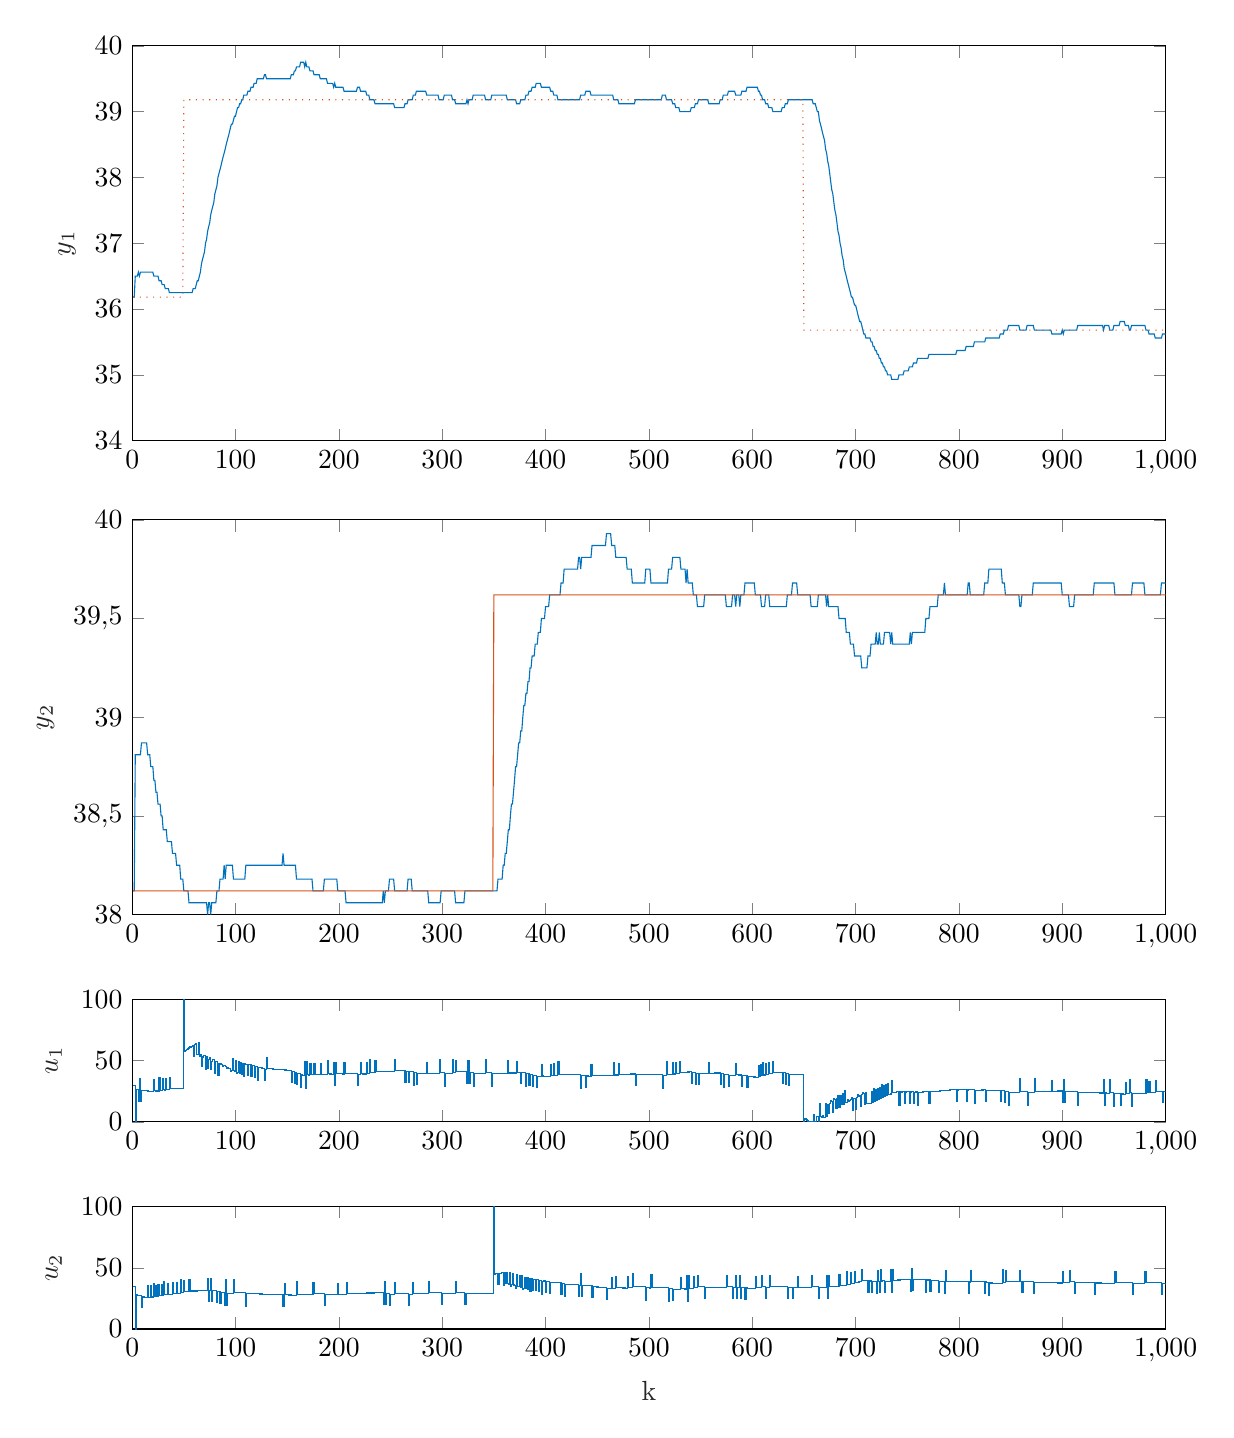
\begin{tikzpicture}

\begin{axis}[%
width=5.167in,
height=0.612in,
at={(0.646in,0.494in)},
scale only axis,
xmin=0,
xmax=1000,
xtick={0,100,200,300,400,500,600,700,800,900,1000},
xlabel style={font=\color{white!15!black}},
xlabel={k},
ymin=0,
ymax=100,
ytick={0,50,100},
ylabel style={font=\color{white!15!black}},
ylabel={$\text{u}_\text{2}$},
axis background/.style={fill=white}
]
\addplot[const plot, color=mycolor1, forget plot] table[row sep=crcr] {%
1	35\\
2	35\\
3	0\\
4	27.87\\
5	27.7167\\
6	27.5633\\
7	27.41\\
8	27.2567\\
9	17.497\\
10	26.33\\
11	26.1633\\
12	25.9967\\
13	25.83\\
14	25.6633\\
15	35.10333\\
16	25.95\\
17	25.7967\\
18	35.25\\
19	26.11\\
20	25.97\\
21	37.0378\\
22	26.4133\\
23	35.89556\\
24	26.7844\\
25	36.28\\
26	27.1822\\
27	27.0844\\
28	36.5933\\
29	27.5089\\
30	38.6322\\
31	28.0633\\
32	27.9944\\
33	27.9256\\
34	37.4633\\
35	28.4078\\
36	28.3522\\
37	28.2967\\
38	28.2411\\
39	37.7922\\
40	28.75\\
41	28.7078\\
42	28.6656\\
43	38.23\\
44	29.2011\\
45	29.1722\\
46	29.1433\\
47	40.3222\\
48	29.8089\\
49	29.7956\\
50	39.3889\\
51	30.3889\\
52	30.3889\\
53	30.3889\\
54	30.3889\\
55	39.9956\\
56	31.0089\\
57	31.0222\\
58	31.0356\\
59	31.0489\\
60	31.0622\\
61	31.0756\\
62	31.0889\\
63	31.1022\\
64	31.1156\\
65	31.1289\\
66	31.1422\\
67	31.1556\\
68	31.1689\\
69	31.1822\\
70	31.1956\\
71	31.2089\\
72	31.2222\\
73	40.8422\\
74	22.262\\
75	31.2756\\
76	40.8956\\
77	22.316\\
78	31.3289\\
79	31.3422\\
80	31.3556\\
81	31.3689\\
82	21.776\\
83	30.7756\\
84	30.7756\\
85	21.169\\
86	30.1556\\
87	30.1422\\
88	30.1289\\
89	18.908\\
90	40.5867\\
91	18.866\\
92	29.3367\\
93	29.3078\\
94	29.2789\\
95	29.25\\
96	29.2211\\
97	29.1922\\
98	40.3711\\
99	29.8578\\
100	29.8444\\
101	29.8311\\
102	29.8178\\
103	29.8044\\
104	29.7911\\
105	29.7778\\
106	29.7644\\
107	29.7511\\
108	29.7378\\
109	29.7244\\
110	18.503\\
111	28.9744\\
112	28.9456\\
113	28.9167\\
114	28.8878\\
115	28.8589\\
116	28.83\\
117	28.8011\\
118	28.7722\\
119	28.7433\\
120	28.7144\\
121	28.6856\\
122	28.6567\\
123	28.6278\\
124	28.5989\\
125	28.57\\
126	28.5411\\
127	28.5122\\
128	28.4833\\
129	28.4544\\
130	28.4256\\
131	28.3967\\
132	28.3678\\
133	28.3389\\
134	28.31\\
135	28.2811\\
136	28.2522\\
137	28.2233\\
138	28.1944\\
139	28.1656\\
140	28.1367\\
141	28.1078\\
142	28.0789\\
143	28.05\\
144	28.0211\\
145	27.9922\\
146	18.357\\
147	36.9211\\
148	27.8922\\
149	27.8633\\
150	27.8344\\
151	27.8056\\
152	27.7767\\
153	27.7478\\
154	27.7189\\
155	27.69\\
156	27.6611\\
157	27.6322\\
158	27.6033\\
159	38.7822\\
160	28.2689\\
161	28.2556\\
162	28.2422\\
163	28.2289\\
164	28.2156\\
165	28.2022\\
166	28.1889\\
167	28.1756\\
168	28.1622\\
169	28.1489\\
170	28.1356\\
171	28.1222\\
172	28.1089\\
173	28.0956\\
174	28.0822\\
175	37.6756\\
176	28.6756\\
177	28.6756\\
178	28.6756\\
179	28.6756\\
180	28.6756\\
181	28.6756\\
182	28.6756\\
183	28.6756\\
184	28.6756\\
185	28.6756\\
186	19.069\\
187	28.0556\\
188	28.0422\\
189	28.0289\\
190	28.0156\\
191	28.0022\\
192	27.9889\\
193	27.9756\\
194	27.9622\\
195	27.9489\\
196	27.9356\\
197	27.9222\\
198	27.9089\\
199	37.5022\\
200	28.5022\\
201	28.5022\\
202	28.5022\\
203	28.5022\\
204	28.5022\\
205	28.5022\\
206	28.5022\\
207	38.1089\\
208	29.1222\\
209	29.1356\\
210	29.1489\\
211	29.1622\\
212	29.1756\\
213	29.1889\\
214	29.2022\\
215	29.2156\\
216	29.2289\\
217	29.2422\\
218	29.2556\\
219	29.2689\\
220	29.2822\\
221	29.2956\\
222	29.3089\\
223	29.3222\\
224	29.3356\\
225	29.3489\\
226	29.3622\\
227	29.3756\\
228	29.3889\\
229	29.4022\\
230	29.4156\\
231	29.4289\\
232	29.4422\\
233	29.4556\\
234	29.4689\\
235	29.4822\\
236	29.4956\\
237	29.5089\\
238	29.5222\\
239	29.5356\\
240	29.5489\\
241	29.5622\\
242	29.5756\\
243	19.982\\
244	38.5889\\
245	19.996\\
246	28.9956\\
247	28.9956\\
248	28.9956\\
249	19.389\\
250	28.3756\\
251	28.3622\\
252	28.3489\\
253	28.3356\\
254	37.9289\\
255	28.9289\\
256	28.9289\\
257	28.9289\\
258	28.9289\\
259	28.9289\\
260	28.9289\\
261	28.9289\\
262	28.9289\\
263	28.9289\\
264	28.9289\\
265	28.9289\\
266	28.9289\\
267	19.322\\
268	28.3089\\
269	28.2956\\
270	28.2822\\
271	37.8756\\
272	28.8756\\
273	28.8756\\
274	28.8756\\
275	28.8756\\
276	28.8756\\
277	28.8756\\
278	28.8756\\
279	28.8756\\
280	28.8756\\
281	28.8756\\
282	28.8756\\
283	28.8756\\
284	28.8756\\
285	28.8756\\
286	28.8756\\
287	38.4822\\
288	29.4956\\
289	29.5089\\
290	29.5222\\
291	29.5356\\
292	29.5489\\
293	29.5622\\
294	29.5756\\
295	29.5889\\
296	29.6022\\
297	29.6156\\
298	29.6289\\
299	20.036\\
300	29.0356\\
301	29.0356\\
302	29.0356\\
303	29.0356\\
304	29.0356\\
305	29.0356\\
306	29.0356\\
307	29.0356\\
308	29.0356\\
309	29.0356\\
310	29.0356\\
311	29.0356\\
312	29.0356\\
313	38.6422\\
314	29.6556\\
315	29.6689\\
316	29.6822\\
317	29.6956\\
318	29.7089\\
319	29.7222\\
320	29.7356\\
321	29.7489\\
322	20.156\\
323	29.1556\\
324	29.1556\\
325	29.1556\\
326	29.1556\\
327	29.1556\\
328	29.1556\\
329	29.1556\\
330	29.1556\\
331	29.1556\\
332	29.1556\\
333	29.1556\\
334	29.1556\\
335	29.1556\\
336	29.1556\\
337	29.1556\\
338	29.1556\\
339	29.1556\\
340	29.1556\\
341	29.1556\\
342	29.1556\\
343	29.1556\\
344	29.1556\\
345	29.1556\\
346	29.1556\\
347	29.1556\\
348	29.1556\\
349	29.1556\\
350	100\\
351	44.6556\\
352	44.9889\\
353	45.322\\
354	36.0489\\
355	45.369\\
356	45.689\\
357	46.009\\
358	46.329\\
359	35.44111\\
360	46.246\\
361	36.9433\\
362	46.234\\
363	36.9189\\
364	36.59\\
365	45.854\\
366	34.911111\\
367	36.0533\\
368	45.289\\
369	35.91778\\
370	35.53333\\
371	33.5344\\
372	44.2278\\
373	34.81444\\
374	34.38778\\
375	43.5544\\
376	34.11444\\
377	43.2678\\
378	32.2133\\
379	33.2444\\
380	42.3689\\
381	32.8867\\
382	41.9978\\
383	32.5022\\
384	41.6\\
385	30.49\\
386	41.0722\\
387	31.5478\\
388	40.6167\\
389	40.6856\\
390	31.1478\\
391	40.2033\\
392	40.2589\\
393	30.7078\\
394	39.75\\
395	39.7922\\
396	28.6267\\
397	39.1533\\
398	39.18\\
399	39.2067\\
400	29.6267\\
401	38.64\\
402	38.6533\\
403	38.6667\\
404	29.0733\\
405	38.0733\\
406	38.0733\\
407	38.0733\\
408	38.0733\\
409	38.0733\\
410	38.0733\\
411	38.0733\\
412	38.0733\\
413	38.0733\\
414	38.0733\\
415	28.4667\\
416	37.4533\\
417	37.44\\
418	26.2189\\
419	36.69\\
420	36.6611\\
421	36.6322\\
422	36.6033\\
423	36.5744\\
424	36.5456\\
425	36.5167\\
426	36.4878\\
427	36.4589\\
428	36.43\\
429	36.4011\\
430	36.3722\\
431	36.3433\\
432	26.7078\\
433	35.66556\\
434	45.23\\
435	26.5944\\
436	35.55222\\
437	35.51\\
438	35.46778\\
439	35.42556\\
440	35.38333\\
441	35.34111\\
442	35.29889\\
443	35.25667\\
444	35.21444\\
445	25.5656\\
446	34.51\\
447	34.45444\\
448	34.39889\\
449	34.34333\\
450	34.28778\\
451	34.23222\\
452	34.17667\\
453	34.12111\\
454	34.06556\\
455	34.01\\
456	33.9544\\
457	33.8989\\
458	33.8433\\
459	24.181\\
460	33.1122\\
461	33.0433\\
462	32.9744\\
463	32.9056\\
464	42.4433\\
465	33.3878\\
466	33.3322\\
467	33.2767\\
468	42.8278\\
469	33.7856\\
470	33.7433\\
471	33.7011\\
472	33.6589\\
473	33.6167\\
474	33.5744\\
475	33.5322\\
476	33.49\\
477	33.4478\\
478	33.4056\\
479	42.97\\
480	33.9411\\
481	33.9122\\
482	33.8833\\
483	33.8544\\
484	45.033\\
485	34.52\\
486	34.50667\\
487	34.49333\\
488	34.48\\
489	34.46667\\
490	34.45333\\
491	34.44\\
492	34.42667\\
493	34.41333\\
494	34.4\\
495	34.38667\\
496	34.37333\\
497	23.152\\
498	33.6233\\
499	33.5944\\
500	33.5656\\
501	33.5367\\
502	44.7156\\
503	34.20222\\
504	34.18889\\
505	34.17556\\
506	34.16222\\
507	34.14889\\
508	34.13556\\
509	34.12222\\
510	34.10889\\
511	34.09556\\
512	34.08222\\
513	34.06889\\
514	34.05556\\
515	34.04222\\
516	34.02889\\
517	34.01556\\
518	34.00222\\
519	22.781\\
520	33.2522\\
521	33.2233\\
522	33.1944\\
523	23.559\\
524	32.5167\\
525	32.4744\\
526	32.4322\\
527	32.39\\
528	32.3478\\
529	32.3056\\
530	32.2633\\
531	41.8278\\
532	32.7989\\
533	32.77\\
534	32.7411\\
535	32.7122\\
536	43.8911\\
537	22.17\\
538	43.8489\\
539	33.3356\\
540	33.3222\\
541	33.3089\\
542	33.2956\\
543	42.8889\\
544	33.8889\\
545	33.8889\\
546	33.8889\\
547	43.4956\\
548	34.50889\\
549	34.52222\\
550	34.53556\\
551	34.54889\\
552	34.56222\\
553	34.57556\\
554	24.982\\
555	33.9822\\
556	33.9822\\
557	33.9822\\
558	33.9822\\
559	33.9822\\
560	33.9822\\
561	33.9822\\
562	33.9822\\
563	33.9822\\
564	33.9822\\
565	33.9822\\
566	33.9822\\
567	33.9822\\
568	33.9822\\
569	33.9822\\
570	33.9822\\
571	33.9822\\
572	33.9822\\
573	33.9822\\
574	33.9822\\
575	43.5889\\
576	34.60222\\
577	34.61556\\
578	34.62889\\
579	34.64222\\
580	34.65556\\
581	25.0622\\
582	34.06222\\
583	34.06222\\
584	43.6689\\
585	25.0756\\
586	34.07556\\
587	34.07556\\
588	43.6822\\
589	25.0889\\
590	34.08889\\
591	34.08889\\
592	34.08889\\
593	24.482\\
594	33.4689\\
595	33.4556\\
596	33.4422\\
597	33.4289\\
598	33.4156\\
599	33.4022\\
600	33.3889\\
601	33.3756\\
602	33.3622\\
603	42.9556\\
604	33.9556\\
605	33.9556\\
606	33.9556\\
607	33.9556\\
608	33.9556\\
609	43.5622\\
610	34.57556\\
611	34.58889\\
612	34.60222\\
613	25.0089\\
614	34.00889\\
615	34.00889\\
616	34.00889\\
617	43.6156\\
618	34.62889\\
619	34.64222\\
620	34.65556\\
621	34.66889\\
622	34.68222\\
623	34.69556\\
624	34.70889\\
625	34.72222\\
626	34.73556\\
627	34.74889\\
628	34.76222\\
629	34.77556\\
630	34.78889\\
631	34.80222\\
632	34.81556\\
633	34.82889\\
634	25.2356\\
635	34.23556\\
636	34.23556\\
637	34.23556\\
638	34.23556\\
639	24.629\\
640	33.6156\\
641	33.6022\\
642	33.5889\\
643	33.5756\\
644	43.1689\\
645	34.16889\\
646	34.16889\\
647	34.16889\\
648	34.16889\\
649	34.16889\\
650	34.16889\\
651	34.16889\\
652	34.16889\\
653	34.16889\\
654	34.16889\\
655	34.16889\\
656	34.16889\\
657	43.7756\\
658	34.78889\\
659	34.80222\\
660	34.81556\\
661	34.82889\\
662	34.84222\\
663	34.85556\\
664	25.2622\\
665	34.26222\\
666	34.26222\\
667	34.26222\\
668	34.26222\\
669	34.26222\\
670	34.26222\\
671	34.26222\\
672	43.8689\\
673	25.2756\\
674	43.8822\\
675	34.89556\\
676	34.908889\\
677	34.922222\\
678	34.935556\\
679	34.948889\\
680	34.962222\\
681	34.975556\\
682	34.988889\\
683	35.0022222\\
684	44.6222\\
685	35.64889\\
686	35.67556\\
687	35.70222\\
688	35.72889\\
689	35.75556\\
690	35.78222\\
691	47.017\\
692	36.5589\\
693	36.6011\\
694	36.6433\\
695	46.292\\
696	37.3478\\
697	37.4033\\
698	37.4589\\
699	47.121\\
700	38.19\\
701	38.2589\\
702	38.3278\\
703	38.3967\\
704	38.4656\\
705	38.5344\\
706	48.21\\
707	39.2922\\
708	39.3744\\
709	39.4567\\
710	39.5389\\
711	39.6211\\
712	30.0967\\
713	39.1656\\
714	39.2344\\
715	29.6967\\
716	38.7522\\
717	38.8078\\
718	38.8633\\
719	38.9189\\
720	29.3678\\
721	48.017\\
722	39.0722\\
723	29.5211\\
724	48.17\\
725	39.2256\\
726	39.2811\\
727	39.3367\\
728	29.7856\\
729	38.8278\\
730	38.87\\
731	38.9122\\
732	38.9544\\
733	38.9967\\
734	48.646\\
735	30.0944\\
736	48.743\\
737	39.7989\\
738	39.8544\\
739	39.91\\
740	39.9656\\
741	40.0211\\
742	40.0767\\
743	40.1322\\
744	40.1878\\
745	40.2433\\
746	40.2989\\
747	40.3544\\
748	40.41\\
749	40.4656\\
750	40.5211\\
751	40.5767\\
752	40.6322\\
753	31.0811\\
754	49.73\\
755	31.1789\\
756	40.2211\\
757	40.2633\\
758	40.3056\\
759	40.3478\\
760	40.39\\
761	40.4322\\
762	40.4744\\
763	40.5167\\
764	40.5589\\
765	40.6011\\
766	40.6433\\
767	40.6856\\
768	29.52\\
769	40.0467\\
770	40.0733\\
771	40.1\\
772	30.52\\
773	39.5333\\
774	39.5467\\
775	39.56\\
776	39.5733\\
777	39.5867\\
778	39.6\\
779	39.6133\\
780	30.02\\
781	39.02\\
782	39.02\\
783	39.02\\
784	39.02\\
785	39.02\\
786	29.4133\\
787	48.007\\
788	39.0067\\
789	39.0067\\
790	39.0067\\
791	39.0067\\
792	39.0067\\
793	39.0067\\
794	39.0067\\
795	39.0067\\
796	39.0067\\
797	39.0067\\
798	39.0067\\
799	39.0067\\
800	39.0067\\
801	39.0067\\
802	39.0067\\
803	39.0067\\
804	39.0067\\
805	39.0067\\
806	39.0067\\
807	39.0067\\
808	39.0067\\
809	29.4\\
810	38.3867\\
811	47.98\\
812	38.98\\
813	38.98\\
814	38.98\\
815	38.98\\
816	38.98\\
817	38.98\\
818	38.98\\
819	38.98\\
820	38.98\\
821	38.98\\
822	38.98\\
823	38.98\\
824	38.98\\
825	29.3733\\
826	38.36\\
827	38.3467\\
828	38.3333\\
829	27.1122\\
830	37.5833\\
831	37.5544\\
832	37.5256\\
833	37.4967\\
834	37.4678\\
835	37.4389\\
836	37.41\\
837	37.3811\\
838	37.3522\\
839	37.3233\\
840	37.2944\\
841	37.2656\\
842	48.444\\
843	37.9311\\
844	37.9178\\
845	47.511\\
846	38.5111\\
847	38.5111\\
848	38.5111\\
849	38.5111\\
850	38.5111\\
851	38.5111\\
852	38.5111\\
853	38.5111\\
854	38.5111\\
855	38.5111\\
856	38.5111\\
857	38.5111\\
858	38.5111\\
859	48.118\\
860	39.1311\\
861	29.5378\\
862	38.5378\\
863	38.5378\\
864	38.5378\\
865	38.5378\\
866	38.5378\\
867	38.5378\\
868	38.5378\\
869	38.5378\\
870	38.5378\\
871	38.5378\\
872	28.9311\\
873	37.9178\\
874	37.9044\\
875	37.8911\\
876	37.8778\\
877	37.8644\\
878	37.8511\\
879	37.8378\\
880	37.8244\\
881	37.8111\\
882	37.7978\\
883	37.7844\\
884	37.7711\\
885	37.7578\\
886	37.7444\\
887	37.7311\\
888	37.7178\\
889	37.7044\\
890	37.6911\\
891	37.6778\\
892	37.6644\\
893	37.6511\\
894	37.6378\\
895	37.6244\\
896	37.6111\\
897	37.5978\\
898	37.5844\\
899	37.5711\\
900	47.164\\
901	38.1644\\
902	38.1644\\
903	38.1644\\
904	38.1644\\
905	38.1644\\
906	38.1644\\
907	47.771\\
908	38.7844\\
909	38.7978\\
910	38.8111\\
911	38.8244\\
912	29.2311\\
913	38.2311\\
914	38.2311\\
915	38.2311\\
916	38.2311\\
917	38.2311\\
918	38.2311\\
919	38.2311\\
920	38.2311\\
921	38.2311\\
922	38.2311\\
923	38.2311\\
924	38.2311\\
925	38.2311\\
926	38.2311\\
927	38.2311\\
928	38.2311\\
929	38.2311\\
930	38.2311\\
931	28.6244\\
932	37.6111\\
933	37.5978\\
934	37.5844\\
935	37.5711\\
936	37.5578\\
937	37.5444\\
938	37.5311\\
939	37.5178\\
940	37.5044\\
941	37.4911\\
942	37.4778\\
943	37.4644\\
944	37.4511\\
945	37.4378\\
946	37.4244\\
947	37.4111\\
948	37.3978\\
949	37.3844\\
950	37.3711\\
951	46.964\\
952	37.9644\\
953	37.9644\\
954	37.9644\\
955	37.9644\\
956	37.9644\\
957	37.9644\\
958	37.9644\\
959	37.9644\\
960	37.9644\\
961	37.9644\\
962	37.9644\\
963	37.9644\\
964	37.9644\\
965	37.9644\\
966	37.9644\\
967	37.9644\\
968	28.3578\\
969	37.3444\\
970	37.3311\\
971	37.3178\\
972	37.3044\\
973	37.2911\\
974	37.2778\\
975	37.2644\\
976	37.2511\\
977	37.2378\\
978	37.2244\\
979	37.2111\\
980	46.804\\
981	37.8044\\
982	37.8044\\
983	37.8044\\
984	37.8044\\
985	37.8044\\
986	37.8044\\
987	37.8044\\
988	37.8044\\
989	37.8044\\
990	37.8044\\
991	37.8044\\
992	37.8044\\
993	37.8044\\
994	37.8044\\
995	37.8044\\
996	28.1978\\
997	37.1844\\
998	37.1711\\
999	37.1578\\
1000	37.1444\\
};
\end{axis}

\begin{axis}[%
width=5.167in,
height=0.612in,
at={(0.646in,1.53in)},
scale only axis,
xmin=0,
xmax=1000,
xtick={0,100,200,300,400,500,600,700,800,900,1000},
ymin=0,
ymax=100,
ytick={0,50,100},
ylabel style={font=\color{white!15!black}},
ylabel={$\text{u}_\text{1}$},
axis background/.style={fill=white}
]
\addplot[const plot, color=mycolor1, forget plot] table[row sep=crcr] {%
1	30\\
2	30\\
3	0\\
4	26.6933\\
5	26.6222\\
6	16.944\\
7	35.4667\\
8	16.789\\
9	25.7044\\
10	25.62\\
11	25.5356\\
12	25.4511\\
13	25.3667\\
14	25.2822\\
15	25.1978\\
16	25.1133\\
17	25.0289\\
18	24.9444\\
19	24.86\\
20	24.7756\\
21	34.2978\\
22	25.2267\\
23	25.1556\\
24	25.0844\\
25	25.0133\\
26	36.15\\
27	25.5944\\
28	25.5389\\
29	35.09\\
30	26.0478\\
31	26.0056\\
32	35.57\\
33	26.5411\\
34	26.5122\\
35	26.4833\\
36	36.0611\\
37	27.0456\\
38	27.03\\
39	27.0144\\
40	26.9989\\
41	26.9833\\
42	26.9678\\
43	26.9522\\
44	26.9367\\
45	26.9211\\
46	26.9056\\
47	26.89\\
48	26.8744\\
49	26.8589\\
50	100\\
51	57.828\\
52	58.479\\
53	59.13\\
54	59.781\\
55	60.432\\
56	61.083\\
57	61.734\\
58	62.386\\
59	53.43\\
60	63.068\\
61	63.706\\
62	54.737\\
63	54.754\\
64	64.366\\
65	53.769\\
66	55.258\\
67	45.627\\
68	52.974\\
69	54.408\\
70	54.328\\
71	43.027\\
72	53.404\\
73	43.662\\
74	50.899\\
75	52.221\\
76	42.423\\
77	49.604\\
78	50.871\\
79	50.624\\
80	39.1567\\
81	49.368\\
82	49.066\\
83	37.5422\\
84	47.698\\
85	47.34\\
86	46.969\\
87	44.983\\
88	46.083\\
89	45.67\\
90	45.243\\
91	43.202\\
92	44.247\\
93	43.778\\
94	43.296\\
95	41.199\\
96	42.188\\
97	51.27\\
98	41.746\\
99	41.208\\
100	50.263\\
101	39.1111\\
102	40.044\\
103	49.071\\
104	39.4911\\
105	48.504\\
106	38.9111\\
107	47.911\\
108	36.7033\\
109	47.188\\
110	47.172\\
111	47.157\\
112	37.5344\\
113	46.506\\
114	46.477\\
115	36.8411\\
116	45.799\\
117	45.757\\
118	36.1078\\
119	45.052\\
120	44.997\\
121	33.7333\\
122	44.162\\
123	44.091\\
124	44.02\\
125	43.949\\
126	43.878\\
127	43.807\\
128	34.1289\\
129	43.044\\
130	52.567\\
131	43.496\\
132	43.424\\
133	43.353\\
134	43.282\\
135	43.211\\
136	43.14\\
137	43.069\\
138	42.998\\
139	42.927\\
140	42.856\\
141	42.784\\
142	42.713\\
143	42.642\\
144	42.571\\
145	42.5\\
146	42.429\\
147	42.358\\
148	42.287\\
149	42.216\\
150	42.144\\
151	42.073\\
152	42.002\\
153	41.931\\
154	32.2533\\
155	41.169\\
156	41.084\\
157	31.3933\\
158	40.296\\
159	30.59111\\
160	39.48\\
161	39.3689\\
162	39.2578\\
163	27.9389\\
164	38.3122\\
165	38.1856\\
166	38.0589\\
167	49.14\\
168	27.3211\\
169	48.902\\
170	38.2911\\
171	38.18\\
172	47.676\\
173	38.5778\\
174	38.48\\
175	38.3822\\
176	47.891\\
177	38.8067\\
178	38.7222\\
179	38.6378\\
180	38.5533\\
181	38.4689\\
182	47.991\\
183	38.92\\
184	38.8489\\
185	38.7778\\
186	38.7067\\
187	38.6356\\
188	38.5644\\
189	49.701\\
190	39.1456\\
191	39.09\\
192	39.0344\\
193	38.9789\\
194	38.9233\\
195	48.474\\
196	29.82556\\
197	48.377\\
198	39.3344\\
199	39.2922\\
200	39.25\\
201	39.2078\\
202	39.1656\\
203	39.1233\\
204	39.0811\\
205	48.646\\
206	39.6167\\
207	39.5878\\
208	39.5589\\
209	39.53\\
210	39.5011\\
211	39.4722\\
212	39.4433\\
213	39.4144\\
214	39.3856\\
215	39.3567\\
216	39.3278\\
217	39.2989\\
218	29.66333\\
219	38.6211\\
220	38.5789\\
221	48.143\\
222	39.1144\\
223	39.0856\\
224	39.0567\\
225	39.0278\\
226	38.9989\\
227	48.577\\
228	39.5611\\
229	39.5456\\
230	50.738\\
231	40.238\\
232	40.238\\
233	40.238\\
234	40.238\\
235	49.844\\
236	40.858\\
237	40.871\\
238	40.884\\
239	40.898\\
240	40.911\\
241	40.924\\
242	40.938\\
243	40.951\\
244	40.964\\
245	40.978\\
246	40.991\\
247	41.004\\
248	41.018\\
249	41.031\\
250	41.044\\
251	41.058\\
252	41.071\\
253	41.084\\
254	50.704\\
255	41.731\\
256	41.758\\
257	41.784\\
258	41.811\\
259	41.838\\
260	41.864\\
261	41.891\\
262	41.918\\
263	41.944\\
264	32.3644\\
265	41.378\\
266	41.391\\
267	31.7978\\
268	40.798\\
269	40.798\\
270	40.798\\
271	40.798\\
272	29.59\\
273	40.074\\
274	40.059\\
275	30.43667\\
276	39.4078\\
277	39.3789\\
278	39.35\\
279	39.3211\\
280	39.2922\\
281	39.2633\\
282	39.2344\\
283	39.2056\\
284	39.1767\\
285	48.754\\
286	39.7389\\
287	39.7233\\
288	39.7078\\
289	39.6922\\
290	39.6767\\
291	39.6611\\
292	39.6456\\
293	39.63\\
294	39.6144\\
295	39.5989\\
296	39.5833\\
297	50.776\\
298	40.276\\
299	40.276\\
300	40.276\\
301	40.276\\
302	29.06778\\
303	39.5522\\
304	39.5367\\
305	39.5211\\
306	39.5056\\
307	39.49\\
308	39.4744\\
309	39.4589\\
310	50.651\\
311	40.151\\
312	40.151\\
313	49.758\\
314	40.771\\
315	40.784\\
316	40.798\\
317	40.811\\
318	40.824\\
319	40.838\\
320	40.851\\
321	40.864\\
322	40.878\\
323	40.891\\
324	31.2978\\
325	49.904\\
326	31.3111\\
327	40.311\\
328	40.311\\
329	40.311\\
330	29.10333\\
331	39.5878\\
332	39.5722\\
333	39.5567\\
334	39.5411\\
335	39.5256\\
336	39.51\\
337	39.4944\\
338	39.4789\\
339	39.4633\\
340	39.4478\\
341	39.4322\\
342	50.624\\
343	40.124\\
344	40.124\\
345	40.124\\
346	40.124\\
347	40.124\\
348	28.9167\\
349	39.4011\\
350	39.3856\\
351	39.37\\
352	39.3544\\
353	39.3389\\
354	39.3233\\
355	39.3078\\
356	39.2922\\
357	39.2767\\
358	39.2611\\
359	39.2456\\
360	39.23\\
361	39.2144\\
362	39.1989\\
363	50.391\\
364	39.8911\\
365	39.8911\\
366	39.8911\\
367	39.8911\\
368	39.8911\\
369	39.8911\\
370	39.8911\\
371	39.8911\\
372	49.498\\
373	40.511\\
374	40.524\\
375	40.538\\
376	30.94444\\
377	39.9444\\
378	39.9444\\
379	39.9444\\
380	39.9444\\
381	28.7367\\
382	39.2211\\
383	39.2056\\
384	29.58333\\
385	38.5544\\
386	38.5256\\
387	28.89\\
388	37.8478\\
389	37.8056\\
390	37.7633\\
391	28.1144\\
392	37.0589\\
393	37.0033\\
394	36.9478\\
395	36.8922\\
396	46.443\\
397	37.4011\\
398	37.3589\\
399	37.3167\\
400	37.2744\\
401	37.2322\\
402	37.19\\
403	37.1478\\
404	37.1056\\
405	46.67\\
406	37.6411\\
407	37.6122\\
408	47.19\\
409	38.1744\\
410	38.1589\\
411	38.1433\\
412	49.336\\
413	38.8356\\
414	38.8356\\
415	38.8356\\
416	38.8356\\
417	38.8356\\
418	38.8356\\
419	38.8356\\
420	38.8356\\
421	38.8356\\
422	38.8356\\
423	38.8356\\
424	38.8356\\
425	38.8356\\
426	38.8356\\
427	38.8356\\
428	38.8356\\
429	38.8356\\
430	38.8356\\
431	38.8356\\
432	38.8356\\
433	38.8356\\
434	27.6278\\
435	38.1122\\
436	38.0967\\
437	38.0811\\
438	38.0656\\
439	28.4433\\
440	37.4144\\
441	37.3856\\
442	37.3567\\
443	37.3278\\
444	46.906\\
445	37.89\\
446	37.8744\\
447	37.8589\\
448	37.8433\\
449	37.8278\\
450	37.8122\\
451	37.7967\\
452	37.7811\\
453	37.7656\\
454	37.75\\
455	37.7344\\
456	37.7189\\
457	37.7033\\
458	37.6878\\
459	37.6722\\
460	37.6567\\
461	37.6411\\
462	37.6256\\
463	37.61\\
464	37.5944\\
465	37.5789\\
466	48.771\\
467	38.2711\\
468	38.2711\\
469	38.2711\\
470	38.2711\\
471	47.878\\
472	38.8911\\
473	38.9044\\
474	38.9178\\
475	38.9311\\
476	38.9444\\
477	38.9578\\
478	38.9711\\
479	38.9844\\
480	38.9978\\
481	39.0111\\
482	39.0244\\
483	39.0378\\
484	39.0511\\
485	39.0644\\
486	39.0778\\
487	29.48444\\
488	38.4844\\
489	38.4844\\
490	38.4844\\
491	38.4844\\
492	38.4844\\
493	38.4844\\
494	38.4844\\
495	38.4844\\
496	38.4844\\
497	38.4844\\
498	38.4844\\
499	38.4844\\
500	38.4844\\
501	38.4844\\
502	38.4844\\
503	38.4844\\
504	38.4844\\
505	38.4844\\
506	38.4844\\
507	38.4844\\
508	38.4844\\
509	38.4844\\
510	38.4844\\
511	38.4844\\
512	38.4844\\
513	27.2767\\
514	37.7611\\
515	37.7456\\
516	37.73\\
517	48.922\\
518	38.4222\\
519	38.4222\\
520	38.4222\\
521	38.4222\\
522	38.4222\\
523	48.029\\
524	39.0422\\
525	39.0556\\
526	48.676\\
527	39.7022\\
528	39.7289\\
529	39.7556\\
530	49.389\\
531	40.429\\
532	40.469\\
533	40.509\\
534	40.549\\
535	40.589\\
536	40.629\\
537	40.669\\
538	40.709\\
539	40.749\\
540	40.789\\
541	31.2222\\
542	40.249\\
543	40.276\\
544	40.302\\
545	30.72222\\
546	39.7356\\
547	39.7489\\
548	30.15556\\
549	39.1556\\
550	39.1556\\
551	39.1556\\
552	39.1556\\
553	39.1556\\
554	39.1556\\
555	39.1556\\
556	39.1556\\
557	39.1556\\
558	48.762\\
559	39.7756\\
560	39.7889\\
561	39.8022\\
562	39.8156\\
563	39.8289\\
564	39.8422\\
565	39.8556\\
566	39.8689\\
567	39.8822\\
568	39.8956\\
569	30.30222\\
570	39.3022\\
571	39.3022\\
572	28.0944\\
573	38.5789\\
574	38.5633\\
575	38.5478\\
576	38.5322\\
577	28.91\\
578	37.8811\\
579	37.8522\\
580	37.8233\\
581	37.7944\\
582	37.7656\\
583	37.7367\\
584	47.314\\
585	38.2989\\
586	38.2833\\
587	38.2678\\
588	38.2522\\
589	38.2367\\
590	28.6144\\
591	37.5856\\
592	37.5567\\
593	37.5278\\
594	37.4989\\
595	27.8633\\
596	36.8211\\
597	36.7789\\
598	36.7367\\
599	36.6944\\
600	36.6522\\
601	36.61\\
602	36.5678\\
603	36.5256\\
604	36.4833\\
605	36.4411\\
606	46.006\\
607	36.9767\\
608	46.554\\
609	37.5389\\
610	48.731\\
611	38.2311\\
612	38.2311\\
613	47.838\\
614	38.8511\\
615	38.8644\\
616	48.484\\
617	39.5111\\
618	39.5378\\
619	39.5644\\
620	49.198\\
621	40.238\\
622	40.278\\
623	40.318\\
624	40.358\\
625	40.398\\
626	40.438\\
627	40.478\\
628	40.518\\
629	30.95111\\
630	39.9778\\
631	40.004\\
632	30.42444\\
633	39.4378\\
634	39.4511\\
635	29.85778\\
636	38.8578\\
637	38.8578\\
638	38.8578\\
639	38.8578\\
640	38.8578\\
641	38.8578\\
642	38.8578\\
643	38.8578\\
644	38.8578\\
645	38.8578\\
646	38.8578\\
647	38.8578\\
648	38.8578\\
649	38.8578\\
650	0\\
651	2.691\\
652	1.913\\
653	1.136\\
654	0.358000000000001\\
655	0\\
656	0\\
657	0\\
658	0\\
659	6.076\\
660	0\\
661	0\\
662	4.389\\
663	4.244\\
664	0\\
665	14.583\\
666	3.981\\
667	3.892\\
668	5.418\\
669	3.858\\
670	3.811\\
671	14.986\\
672	4.481\\
673	14.097\\
674	6.733\\
675	14.891\\
676	17.177\\
677	16.39\\
678	7.523\\
679	18.878\\
680	18.16\\
681	10.963\\
682	19.288\\
683	21.74\\
684	11.513\\
685	21.4067\\
686	14.321\\
687	22.7567\\
688	14.112\\
689	25.6889\\
690	15.587\\
691	15.998\\
692	18.023\\
693	16.963\\
694	17.417\\
695	17.883\\
696	19.964\\
697	9.353\\
698	18.849\\
699	19.358\\
700	10.273\\
701	19.796\\
702	21.9322\\
703	20.9833\\
704	21.5478\\
705	12.519\\
706	22.0967\\
707	24.2889\\
708	23.3956\\
709	14.409\\
710	24.0289\\
711	15.056\\
712	15.082\\
713	15.109\\
714	15.136\\
715	24.7689\\
716	15.809\\
717	27.0567\\
718	16.612\\
719	26.2744\\
720	17.343\\
721	27.0189\\
722	18.101\\
723	27.79\\
724	18.886\\
725	30.18889\\
726	19.8\\
727	29.51778\\
728	20.6422\\
729	30.37333\\
730	21.5111\\
731	31.2556\\
732	22.4067\\
733	22.5578\\
734	22.7089\\
735	34.0678\\
736	23.7344\\
737	23.9011\\
738	24.0678\\
739	24.2344\\
740	24.4011\\
741	24.5678\\
742	13.527\\
743	24.1778\\
744	24.3289\\
745	24.48\\
746	24.6311\\
747	15.176\\
748	24.3133\\
749	24.4511\\
750	24.5889\\
751	24.7267\\
752	15.258\\
753	24.3822\\
754	24.5067\\
755	24.6311\\
756	15.149\\
757	24.26\\
758	24.3711\\
759	24.4822\\
760	13.386\\
761	23.9811\\
762	24.0767\\
763	24.1722\\
764	24.2678\\
765	24.3633\\
766	24.4589\\
767	24.5544\\
768	24.65\\
769	24.7456\\
770	24.8411\\
771	15.33\\
772	24.4122\\
773	24.4944\\
774	24.5767\\
775	24.6589\\
776	24.7411\\
777	24.8233\\
778	24.9056\\
779	24.9878\\
780	25.07\\
781	25.1522\\
782	25.2344\\
783	25.3167\\
784	25.3989\\
785	25.4811\\
786	25.5633\\
787	25.6456\\
788	25.7278\\
789	25.81\\
790	25.8922\\
791	25.9744\\
792	26.0567\\
793	26.1389\\
794	26.2211\\
795	26.3033\\
796	26.3856\\
797	26.4678\\
798	16.943\\
799	26.0122\\
800	26.0811\\
801	26.15\\
802	26.2189\\
803	26.2878\\
804	26.3567\\
805	26.4256\\
806	26.4944\\
807	16.957\\
808	26.0122\\
809	26.0678\\
810	26.1233\\
811	26.1789\\
812	26.2344\\
813	26.29\\
814	26.3456\\
815	15.193\\
816	25.7333\\
817	25.7733\\
818	25.8133\\
819	25.8533\\
820	25.8933\\
821	25.9333\\
822	25.9733\\
823	26.0133\\
824	26.0533\\
825	26.0933\\
826	16.527\\
827	25.5533\\
828	25.58\\
829	25.6067\\
830	25.6333\\
831	25.66\\
832	25.6867\\
833	25.7133\\
834	25.74\\
835	25.7667\\
836	25.7933\\
837	25.82\\
838	25.8467\\
839	25.8733\\
840	16.293\\
841	25.3067\\
842	25.32\\
843	25.3333\\
844	15.74\\
845	24.74\\
846	24.74\\
847	24.74\\
848	13.532\\
849	24.0167\\
850	24.0011\\
851	23.9856\\
852	23.97\\
853	23.9544\\
854	23.9389\\
855	23.9233\\
856	23.9078\\
857	23.8922\\
858	23.8767\\
859	35.0689\\
860	24.5689\\
861	24.5689\\
862	24.5689\\
863	24.5689\\
864	24.5689\\
865	24.5689\\
866	13.361\\
867	23.8456\\
868	23.83\\
869	23.8144\\
870	23.7989\\
871	23.7833\\
872	23.7678\\
873	34.96\\
874	24.46\\
875	24.46\\
876	24.46\\
877	24.46\\
878	24.46\\
879	24.46\\
880	24.46\\
881	24.46\\
882	24.46\\
883	24.46\\
884	24.46\\
885	24.46\\
886	24.46\\
887	24.46\\
888	24.46\\
889	24.46\\
890	34.0667\\
891	25.08\\
892	25.0933\\
893	25.1067\\
894	25.12\\
895	25.1333\\
896	25.1467\\
897	25.16\\
898	25.1733\\
899	25.1867\\
900	15.593\\
901	34.2\\
902	15.607\\
903	24.6067\\
904	24.6067\\
905	24.6067\\
906	24.6067\\
907	24.6067\\
908	24.6067\\
909	24.6067\\
910	24.6067\\
911	24.6067\\
912	24.6067\\
913	24.6067\\
914	24.6067\\
915	13.399\\
916	23.8833\\
917	23.8678\\
918	23.8522\\
919	23.8367\\
920	23.8211\\
921	23.8056\\
922	23.79\\
923	23.7744\\
924	23.7589\\
925	23.7433\\
926	23.7278\\
927	23.7122\\
928	23.6967\\
929	23.6811\\
930	23.6656\\
931	23.65\\
932	23.6344\\
933	23.6189\\
934	23.6033\\
935	23.5878\\
936	23.5722\\
937	23.5567\\
938	23.5411\\
939	23.5256\\
940	34.7178\\
941	13.01\\
942	23.4944\\
943	23.4789\\
944	23.4633\\
945	23.4478\\
946	34.64\\
947	24.14\\
948	24.14\\
949	24.14\\
950	12.932\\
951	23.4167\\
952	23.4011\\
953	23.3856\\
954	23.37\\
955	23.3544\\
956	13.732\\
957	22.7033\\
958	22.6744\\
959	22.6456\\
960	22.6167\\
961	32.1944\\
962	23.1789\\
963	23.1633\\
964	23.1478\\
965	34.34\\
966	23.84\\
967	12.632\\
968	23.1167\\
969	23.1011\\
970	23.0856\\
971	23.07\\
972	23.0544\\
973	23.0389\\
974	23.0233\\
975	23.0078\\
976	22.9922\\
977	22.9767\\
978	22.9611\\
979	22.9456\\
980	22.93\\
981	34.1222\\
982	23.6222\\
983	23.6222\\
984	33.2289\\
985	24.2422\\
986	24.2556\\
987	24.2689\\
988	24.2822\\
989	24.2956\\
990	33.9156\\
991	24.9422\\
992	24.9689\\
993	24.9956\\
994	25.0222\\
995	25.0489\\
996	25.0756\\
997	15.496\\
998	24.5089\\
999	24.5222\\
1000	24.5356\\
};
\end{axis}

\begin{axis}[%
width=5.167in,
height=1.974in,
at={(0.646in,2.566in)},
scale only axis,
xmin=0,
xmax=1000,
xtick={0,100,200,300,400,500,600,700,800,900,1000},
ymin=38,
ymax=40,
ytick={38,38.5,39,39.5,40},
yticklabels={{38},{38,5},{39},{39,5},{40}},
ylabel style={font=\color{white!15!black}},
ylabel={$\text{y}_\text{2}$},
axis background/.style={fill=white}
]
\addplot [color=mycolor1, forget plot]
  table[row sep=crcr]{%
1	38.12\\
2	38.12\\
3	38.81\\
4	38.81\\
5	38.81\\
6	38.81\\
7	38.81\\
8	38.81\\
9	38.87\\
10	38.87\\
11	38.87\\
12	38.87\\
13	38.87\\
14	38.87\\
15	38.81\\
16	38.81\\
17	38.81\\
18	38.75\\
19	38.75\\
20	38.75\\
21	38.68\\
22	38.68\\
23	38.62\\
24	38.62\\
25	38.56\\
26	38.56\\
27	38.56\\
28	38.5\\
29	38.5\\
30	38.43\\
31	38.43\\
32	38.43\\
33	38.43\\
34	38.37\\
35	38.37\\
36	38.37\\
37	38.37\\
38	38.37\\
39	38.31\\
40	38.31\\
41	38.31\\
42	38.31\\
43	38.25\\
44	38.25\\
45	38.25\\
46	38.25\\
47	38.18\\
48	38.18\\
49	38.18\\
50	38.12\\
51	38.12\\
52	38.12\\
53	38.12\\
54	38.12\\
55	38.06\\
56	38.06\\
57	38.06\\
58	38.06\\
59	38.06\\
60	38.06\\
61	38.06\\
62	38.06\\
63	38.06\\
64	38.06\\
65	38.06\\
66	38.06\\
67	38.06\\
68	38.06\\
69	38.06\\
70	38.06\\
71	38.06\\
72	38.06\\
73	38\\
74	38.06\\
75	38.06\\
76	38\\
77	38.06\\
78	38.06\\
79	38.06\\
80	38.06\\
81	38.06\\
82	38.12\\
83	38.12\\
84	38.12\\
85	38.18\\
86	38.18\\
87	38.18\\
88	38.18\\
89	38.25\\
90	38.18\\
91	38.25\\
92	38.25\\
93	38.25\\
94	38.25\\
95	38.25\\
96	38.25\\
97	38.25\\
98	38.18\\
99	38.18\\
100	38.18\\
101	38.18\\
102	38.18\\
103	38.18\\
104	38.18\\
105	38.18\\
106	38.18\\
107	38.18\\
108	38.18\\
109	38.18\\
110	38.25\\
111	38.25\\
112	38.25\\
113	38.25\\
114	38.25\\
115	38.25\\
116	38.25\\
117	38.25\\
118	38.25\\
119	38.25\\
120	38.25\\
121	38.25\\
122	38.25\\
123	38.25\\
124	38.25\\
125	38.25\\
126	38.25\\
127	38.25\\
128	38.25\\
129	38.25\\
130	38.25\\
131	38.25\\
132	38.25\\
133	38.25\\
134	38.25\\
135	38.25\\
136	38.25\\
137	38.25\\
138	38.25\\
139	38.25\\
140	38.25\\
141	38.25\\
142	38.25\\
143	38.25\\
144	38.25\\
145	38.25\\
146	38.31\\
147	38.25\\
148	38.25\\
149	38.25\\
150	38.25\\
151	38.25\\
152	38.25\\
153	38.25\\
154	38.25\\
155	38.25\\
156	38.25\\
157	38.25\\
158	38.25\\
159	38.18\\
160	38.18\\
161	38.18\\
162	38.18\\
163	38.18\\
164	38.18\\
165	38.18\\
166	38.18\\
167	38.18\\
168	38.18\\
169	38.18\\
170	38.18\\
171	38.18\\
172	38.18\\
173	38.18\\
174	38.18\\
175	38.12\\
176	38.12\\
177	38.12\\
178	38.12\\
179	38.12\\
180	38.12\\
181	38.12\\
182	38.12\\
183	38.12\\
184	38.12\\
185	38.12\\
186	38.18\\
187	38.18\\
188	38.18\\
189	38.18\\
190	38.18\\
191	38.18\\
192	38.18\\
193	38.18\\
194	38.18\\
195	38.18\\
196	38.18\\
197	38.18\\
198	38.18\\
199	38.12\\
200	38.12\\
201	38.12\\
202	38.12\\
203	38.12\\
204	38.12\\
205	38.12\\
206	38.12\\
207	38.06\\
208	38.06\\
209	38.06\\
210	38.06\\
211	38.06\\
212	38.06\\
213	38.06\\
214	38.06\\
215	38.06\\
216	38.06\\
217	38.06\\
218	38.06\\
219	38.06\\
220	38.06\\
221	38.06\\
222	38.06\\
223	38.06\\
224	38.06\\
225	38.06\\
226	38.06\\
227	38.06\\
228	38.06\\
229	38.06\\
230	38.06\\
231	38.06\\
232	38.06\\
233	38.06\\
234	38.06\\
235	38.06\\
236	38.06\\
237	38.06\\
238	38.06\\
239	38.06\\
240	38.06\\
241	38.06\\
242	38.06\\
243	38.12\\
244	38.06\\
245	38.12\\
246	38.12\\
247	38.12\\
248	38.12\\
249	38.18\\
250	38.18\\
251	38.18\\
252	38.18\\
253	38.18\\
254	38.12\\
255	38.12\\
256	38.12\\
257	38.12\\
258	38.12\\
259	38.12\\
260	38.12\\
261	38.12\\
262	38.12\\
263	38.12\\
264	38.12\\
265	38.12\\
266	38.12\\
267	38.18\\
268	38.18\\
269	38.18\\
270	38.18\\
271	38.12\\
272	38.12\\
273	38.12\\
274	38.12\\
275	38.12\\
276	38.12\\
277	38.12\\
278	38.12\\
279	38.12\\
280	38.12\\
281	38.12\\
282	38.12\\
283	38.12\\
284	38.12\\
285	38.12\\
286	38.12\\
287	38.06\\
288	38.06\\
289	38.06\\
290	38.06\\
291	38.06\\
292	38.06\\
293	38.06\\
294	38.06\\
295	38.06\\
296	38.06\\
297	38.06\\
298	38.06\\
299	38.12\\
300	38.12\\
301	38.12\\
302	38.12\\
303	38.12\\
304	38.12\\
305	38.12\\
306	38.12\\
307	38.12\\
308	38.12\\
309	38.12\\
310	38.12\\
311	38.12\\
312	38.12\\
313	38.06\\
314	38.06\\
315	38.06\\
316	38.06\\
317	38.06\\
318	38.06\\
319	38.06\\
320	38.06\\
321	38.06\\
322	38.12\\
323	38.12\\
324	38.12\\
325	38.12\\
326	38.12\\
327	38.12\\
328	38.12\\
329	38.12\\
330	38.12\\
331	38.12\\
332	38.12\\
333	38.12\\
334	38.12\\
335	38.12\\
336	38.12\\
337	38.12\\
338	38.12\\
339	38.12\\
340	38.12\\
341	38.12\\
342	38.12\\
343	38.12\\
344	38.12\\
345	38.12\\
346	38.12\\
347	38.12\\
348	38.12\\
349	38.12\\
350	38.12\\
351	38.12\\
352	38.12\\
353	38.12\\
354	38.18\\
355	38.18\\
356	38.18\\
357	38.18\\
358	38.18\\
359	38.25\\
360	38.25\\
361	38.31\\
362	38.31\\
363	38.37\\
364	38.43\\
365	38.43\\
366	38.5\\
367	38.56\\
368	38.56\\
369	38.62\\
370	38.68\\
371	38.75\\
372	38.75\\
373	38.81\\
374	38.87\\
375	38.87\\
376	38.93\\
377	38.93\\
378	39\\
379	39.06\\
380	39.06\\
381	39.12\\
382	39.12\\
383	39.18\\
384	39.18\\
385	39.25\\
386	39.25\\
387	39.31\\
388	39.31\\
389	39.31\\
390	39.37\\
391	39.37\\
392	39.37\\
393	39.43\\
394	39.43\\
395	39.43\\
396	39.5\\
397	39.5\\
398	39.5\\
399	39.5\\
400	39.56\\
401	39.56\\
402	39.56\\
403	39.56\\
404	39.62\\
405	39.62\\
406	39.62\\
407	39.62\\
408	39.62\\
409	39.62\\
410	39.62\\
411	39.62\\
412	39.62\\
413	39.62\\
414	39.62\\
415	39.68\\
416	39.68\\
417	39.68\\
418	39.75\\
419	39.75\\
420	39.75\\
421	39.75\\
422	39.75\\
423	39.75\\
424	39.75\\
425	39.75\\
426	39.75\\
427	39.75\\
428	39.75\\
429	39.75\\
430	39.75\\
431	39.75\\
432	39.81\\
433	39.81\\
434	39.75\\
435	39.81\\
436	39.81\\
437	39.81\\
438	39.81\\
439	39.81\\
440	39.81\\
441	39.81\\
442	39.81\\
443	39.81\\
444	39.81\\
445	39.87\\
446	39.87\\
447	39.87\\
448	39.87\\
449	39.87\\
450	39.87\\
451	39.87\\
452	39.87\\
453	39.87\\
454	39.87\\
455	39.87\\
456	39.87\\
457	39.87\\
458	39.87\\
459	39.93\\
460	39.93\\
461	39.93\\
462	39.93\\
463	39.93\\
464	39.87\\
465	39.87\\
466	39.87\\
467	39.87\\
468	39.81\\
469	39.81\\
470	39.81\\
471	39.81\\
472	39.81\\
473	39.81\\
474	39.81\\
475	39.81\\
476	39.81\\
477	39.81\\
478	39.81\\
479	39.75\\
480	39.75\\
481	39.75\\
482	39.75\\
483	39.75\\
484	39.68\\
485	39.68\\
486	39.68\\
487	39.68\\
488	39.68\\
489	39.68\\
490	39.68\\
491	39.68\\
492	39.68\\
493	39.68\\
494	39.68\\
495	39.68\\
496	39.68\\
497	39.75\\
498	39.75\\
499	39.75\\
500	39.75\\
501	39.75\\
502	39.68\\
503	39.68\\
504	39.68\\
505	39.68\\
506	39.68\\
507	39.68\\
508	39.68\\
509	39.68\\
510	39.68\\
511	39.68\\
512	39.68\\
513	39.68\\
514	39.68\\
515	39.68\\
516	39.68\\
517	39.68\\
518	39.68\\
519	39.75\\
520	39.75\\
521	39.75\\
522	39.75\\
523	39.81\\
524	39.81\\
525	39.81\\
526	39.81\\
527	39.81\\
528	39.81\\
529	39.81\\
530	39.81\\
531	39.75\\
532	39.75\\
533	39.75\\
534	39.75\\
535	39.75\\
536	39.68\\
537	39.75\\
538	39.68\\
539	39.68\\
540	39.68\\
541	39.68\\
542	39.68\\
543	39.62\\
544	39.62\\
545	39.62\\
546	39.62\\
547	39.56\\
548	39.56\\
549	39.56\\
550	39.56\\
551	39.56\\
552	39.56\\
553	39.56\\
554	39.62\\
555	39.62\\
556	39.62\\
557	39.62\\
558	39.62\\
559	39.62\\
560	39.62\\
561	39.62\\
562	39.62\\
563	39.62\\
564	39.62\\
565	39.62\\
566	39.62\\
567	39.62\\
568	39.62\\
569	39.62\\
570	39.62\\
571	39.62\\
572	39.62\\
573	39.62\\
574	39.62\\
575	39.56\\
576	39.56\\
577	39.56\\
578	39.56\\
579	39.56\\
580	39.56\\
581	39.62\\
582	39.62\\
583	39.62\\
584	39.56\\
585	39.62\\
586	39.62\\
587	39.62\\
588	39.56\\
589	39.62\\
590	39.62\\
591	39.62\\
592	39.62\\
593	39.68\\
594	39.68\\
595	39.68\\
596	39.68\\
597	39.68\\
598	39.68\\
599	39.68\\
600	39.68\\
601	39.68\\
602	39.68\\
603	39.62\\
604	39.62\\
605	39.62\\
606	39.62\\
607	39.62\\
608	39.62\\
609	39.56\\
610	39.56\\
611	39.56\\
612	39.56\\
613	39.62\\
614	39.62\\
615	39.62\\
616	39.62\\
617	39.56\\
618	39.56\\
619	39.56\\
620	39.56\\
621	39.56\\
622	39.56\\
623	39.56\\
624	39.56\\
625	39.56\\
626	39.56\\
627	39.56\\
628	39.56\\
629	39.56\\
630	39.56\\
631	39.56\\
632	39.56\\
633	39.56\\
634	39.62\\
635	39.62\\
636	39.62\\
637	39.62\\
638	39.62\\
639	39.68\\
640	39.68\\
641	39.68\\
642	39.68\\
643	39.68\\
644	39.62\\
645	39.62\\
646	39.62\\
647	39.62\\
648	39.62\\
649	39.62\\
650	39.62\\
651	39.62\\
652	39.62\\
653	39.62\\
654	39.62\\
655	39.62\\
656	39.62\\
657	39.56\\
658	39.56\\
659	39.56\\
660	39.56\\
661	39.56\\
662	39.56\\
663	39.56\\
664	39.62\\
665	39.62\\
666	39.62\\
667	39.62\\
668	39.62\\
669	39.62\\
670	39.62\\
671	39.62\\
672	39.56\\
673	39.62\\
674	39.56\\
675	39.56\\
676	39.56\\
677	39.56\\
678	39.56\\
679	39.56\\
680	39.56\\
681	39.56\\
682	39.56\\
683	39.56\\
684	39.5\\
685	39.5\\
686	39.5\\
687	39.5\\
688	39.5\\
689	39.5\\
690	39.5\\
691	39.43\\
692	39.43\\
693	39.43\\
694	39.43\\
695	39.37\\
696	39.37\\
697	39.37\\
698	39.37\\
699	39.31\\
700	39.31\\
701	39.31\\
702	39.31\\
703	39.31\\
704	39.31\\
705	39.31\\
706	39.25\\
707	39.25\\
708	39.25\\
709	39.25\\
710	39.25\\
711	39.25\\
712	39.31\\
713	39.31\\
714	39.31\\
715	39.37\\
716	39.37\\
717	39.37\\
718	39.37\\
719	39.37\\
720	39.43\\
721	39.37\\
722	39.37\\
723	39.43\\
724	39.37\\
725	39.37\\
726	39.37\\
727	39.37\\
728	39.43\\
729	39.43\\
730	39.43\\
731	39.43\\
732	39.43\\
733	39.43\\
734	39.37\\
735	39.43\\
736	39.37\\
737	39.37\\
738	39.37\\
739	39.37\\
740	39.37\\
741	39.37\\
742	39.37\\
743	39.37\\
744	39.37\\
745	39.37\\
746	39.37\\
747	39.37\\
748	39.37\\
749	39.37\\
750	39.37\\
751	39.37\\
752	39.37\\
753	39.43\\
754	39.37\\
755	39.43\\
756	39.43\\
757	39.43\\
758	39.43\\
759	39.43\\
760	39.43\\
761	39.43\\
762	39.43\\
763	39.43\\
764	39.43\\
765	39.43\\
766	39.43\\
767	39.43\\
768	39.5\\
769	39.5\\
770	39.5\\
771	39.5\\
772	39.56\\
773	39.56\\
774	39.56\\
775	39.56\\
776	39.56\\
777	39.56\\
778	39.56\\
779	39.56\\
780	39.62\\
781	39.62\\
782	39.62\\
783	39.62\\
784	39.62\\
785	39.62\\
786	39.68\\
787	39.62\\
788	39.62\\
789	39.62\\
790	39.62\\
791	39.62\\
792	39.62\\
793	39.62\\
794	39.62\\
795	39.62\\
796	39.62\\
797	39.62\\
798	39.62\\
799	39.62\\
800	39.62\\
801	39.62\\
802	39.62\\
803	39.62\\
804	39.62\\
805	39.62\\
806	39.62\\
807	39.62\\
808	39.62\\
809	39.68\\
810	39.68\\
811	39.62\\
812	39.62\\
813	39.62\\
814	39.62\\
815	39.62\\
816	39.62\\
817	39.62\\
818	39.62\\
819	39.62\\
820	39.62\\
821	39.62\\
822	39.62\\
823	39.62\\
824	39.62\\
825	39.68\\
826	39.68\\
827	39.68\\
828	39.68\\
829	39.75\\
830	39.75\\
831	39.75\\
832	39.75\\
833	39.75\\
834	39.75\\
835	39.75\\
836	39.75\\
837	39.75\\
838	39.75\\
839	39.75\\
840	39.75\\
841	39.75\\
842	39.68\\
843	39.68\\
844	39.68\\
845	39.62\\
846	39.62\\
847	39.62\\
848	39.62\\
849	39.62\\
850	39.62\\
851	39.62\\
852	39.62\\
853	39.62\\
854	39.62\\
855	39.62\\
856	39.62\\
857	39.62\\
858	39.62\\
859	39.56\\
860	39.56\\
861	39.62\\
862	39.62\\
863	39.62\\
864	39.62\\
865	39.62\\
866	39.62\\
867	39.62\\
868	39.62\\
869	39.62\\
870	39.62\\
871	39.62\\
872	39.68\\
873	39.68\\
874	39.68\\
875	39.68\\
876	39.68\\
877	39.68\\
878	39.68\\
879	39.68\\
880	39.68\\
881	39.68\\
882	39.68\\
883	39.68\\
884	39.68\\
885	39.68\\
886	39.68\\
887	39.68\\
888	39.68\\
889	39.68\\
890	39.68\\
891	39.68\\
892	39.68\\
893	39.68\\
894	39.68\\
895	39.68\\
896	39.68\\
897	39.68\\
898	39.68\\
899	39.68\\
900	39.62\\
901	39.62\\
902	39.62\\
903	39.62\\
904	39.62\\
905	39.62\\
906	39.62\\
907	39.56\\
908	39.56\\
909	39.56\\
910	39.56\\
911	39.56\\
912	39.62\\
913	39.62\\
914	39.62\\
915	39.62\\
916	39.62\\
917	39.62\\
918	39.62\\
919	39.62\\
920	39.62\\
921	39.62\\
922	39.62\\
923	39.62\\
924	39.62\\
925	39.62\\
926	39.62\\
927	39.62\\
928	39.62\\
929	39.62\\
930	39.62\\
931	39.68\\
932	39.68\\
933	39.68\\
934	39.68\\
935	39.68\\
936	39.68\\
937	39.68\\
938	39.68\\
939	39.68\\
940	39.68\\
941	39.68\\
942	39.68\\
943	39.68\\
944	39.68\\
945	39.68\\
946	39.68\\
947	39.68\\
948	39.68\\
949	39.68\\
950	39.68\\
951	39.62\\
952	39.62\\
953	39.62\\
954	39.62\\
955	39.62\\
956	39.62\\
957	39.62\\
958	39.62\\
959	39.62\\
960	39.62\\
961	39.62\\
962	39.62\\
963	39.62\\
964	39.62\\
965	39.62\\
966	39.62\\
967	39.62\\
968	39.68\\
969	39.68\\
970	39.68\\
971	39.68\\
972	39.68\\
973	39.68\\
974	39.68\\
975	39.68\\
976	39.68\\
977	39.68\\
978	39.68\\
979	39.68\\
980	39.62\\
981	39.62\\
982	39.62\\
983	39.62\\
984	39.62\\
985	39.62\\
986	39.62\\
987	39.62\\
988	39.62\\
989	39.62\\
990	39.62\\
991	39.62\\
992	39.62\\
993	39.62\\
994	39.62\\
995	39.62\\
996	39.68\\
997	39.68\\
998	39.68\\
999	39.68\\
1000	39.68\\
};
\addplot [color=mycolor2, forget plot]
  table[row sep=crcr]{%
1	38.12\\
2	38.12\\
3	38.12\\
4	38.12\\
5	38.12\\
6	38.12\\
7	38.12\\
8	38.12\\
9	38.12\\
10	38.12\\
11	38.12\\
12	38.12\\
13	38.12\\
14	38.12\\
15	38.12\\
16	38.12\\
17	38.12\\
18	38.12\\
19	38.12\\
20	38.12\\
21	38.12\\
22	38.12\\
23	38.12\\
24	38.12\\
25	38.12\\
26	38.12\\
27	38.12\\
28	38.12\\
29	38.12\\
30	38.12\\
31	38.12\\
32	38.12\\
33	38.12\\
34	38.12\\
35	38.12\\
36	38.12\\
37	38.12\\
38	38.12\\
39	38.12\\
40	38.12\\
41	38.12\\
42	38.12\\
43	38.12\\
44	38.12\\
45	38.12\\
46	38.12\\
47	38.12\\
48	38.12\\
49	38.12\\
50	38.12\\
51	38.12\\
52	38.12\\
53	38.12\\
54	38.12\\
55	38.12\\
56	38.12\\
57	38.12\\
58	38.12\\
59	38.12\\
60	38.12\\
61	38.12\\
62	38.12\\
63	38.12\\
64	38.12\\
65	38.12\\
66	38.12\\
67	38.12\\
68	38.12\\
69	38.12\\
70	38.12\\
71	38.12\\
72	38.12\\
73	38.12\\
74	38.12\\
75	38.12\\
76	38.12\\
77	38.12\\
78	38.12\\
79	38.12\\
80	38.12\\
81	38.12\\
82	38.12\\
83	38.12\\
84	38.12\\
85	38.12\\
86	38.12\\
87	38.12\\
88	38.12\\
89	38.12\\
90	38.12\\
91	38.12\\
92	38.12\\
93	38.12\\
94	38.12\\
95	38.12\\
96	38.12\\
97	38.12\\
98	38.12\\
99	38.12\\
100	38.12\\
101	38.12\\
102	38.12\\
103	38.12\\
104	38.12\\
105	38.12\\
106	38.12\\
107	38.12\\
108	38.12\\
109	38.12\\
110	38.12\\
111	38.12\\
112	38.12\\
113	38.12\\
114	38.12\\
115	38.12\\
116	38.12\\
117	38.12\\
118	38.12\\
119	38.12\\
120	38.12\\
121	38.12\\
122	38.12\\
123	38.12\\
124	38.12\\
125	38.12\\
126	38.12\\
127	38.12\\
128	38.12\\
129	38.12\\
130	38.12\\
131	38.12\\
132	38.12\\
133	38.12\\
134	38.12\\
135	38.12\\
136	38.12\\
137	38.12\\
138	38.12\\
139	38.12\\
140	38.12\\
141	38.12\\
142	38.12\\
143	38.12\\
144	38.12\\
145	38.12\\
146	38.12\\
147	38.12\\
148	38.12\\
149	38.12\\
150	38.12\\
151	38.12\\
152	38.12\\
153	38.12\\
154	38.12\\
155	38.12\\
156	38.12\\
157	38.12\\
158	38.12\\
159	38.12\\
160	38.12\\
161	38.12\\
162	38.12\\
163	38.12\\
164	38.12\\
165	38.12\\
166	38.12\\
167	38.12\\
168	38.12\\
169	38.12\\
170	38.12\\
171	38.12\\
172	38.12\\
173	38.12\\
174	38.12\\
175	38.12\\
176	38.12\\
177	38.12\\
178	38.12\\
179	38.12\\
180	38.12\\
181	38.12\\
182	38.12\\
183	38.12\\
184	38.12\\
185	38.12\\
186	38.12\\
187	38.12\\
188	38.12\\
189	38.12\\
190	38.12\\
191	38.12\\
192	38.12\\
193	38.12\\
194	38.12\\
195	38.12\\
196	38.12\\
197	38.12\\
198	38.12\\
199	38.12\\
200	38.12\\
201	38.12\\
202	38.12\\
203	38.12\\
204	38.12\\
205	38.12\\
206	38.12\\
207	38.12\\
208	38.12\\
209	38.12\\
210	38.12\\
211	38.12\\
212	38.12\\
213	38.12\\
214	38.12\\
215	38.12\\
216	38.12\\
217	38.12\\
218	38.12\\
219	38.12\\
220	38.12\\
221	38.12\\
222	38.12\\
223	38.12\\
224	38.12\\
225	38.12\\
226	38.12\\
227	38.12\\
228	38.12\\
229	38.12\\
230	38.12\\
231	38.12\\
232	38.12\\
233	38.12\\
234	38.12\\
235	38.12\\
236	38.12\\
237	38.12\\
238	38.12\\
239	38.12\\
240	38.12\\
241	38.12\\
242	38.12\\
243	38.12\\
244	38.12\\
245	38.12\\
246	38.12\\
247	38.12\\
248	38.12\\
249	38.12\\
250	38.12\\
251	38.12\\
252	38.12\\
253	38.12\\
254	38.12\\
255	38.12\\
256	38.12\\
257	38.12\\
258	38.12\\
259	38.12\\
260	38.12\\
261	38.12\\
262	38.12\\
263	38.12\\
264	38.12\\
265	38.12\\
266	38.12\\
267	38.12\\
268	38.12\\
269	38.12\\
270	38.12\\
271	38.12\\
272	38.12\\
273	38.12\\
274	38.12\\
275	38.12\\
276	38.12\\
277	38.12\\
278	38.12\\
279	38.12\\
280	38.12\\
281	38.12\\
282	38.12\\
283	38.12\\
284	38.12\\
285	38.12\\
286	38.12\\
287	38.12\\
288	38.12\\
289	38.12\\
290	38.12\\
291	38.12\\
292	38.12\\
293	38.12\\
294	38.12\\
295	38.12\\
296	38.12\\
297	38.12\\
298	38.12\\
299	38.12\\
300	38.12\\
301	38.12\\
302	38.12\\
303	38.12\\
304	38.12\\
305	38.12\\
306	38.12\\
307	38.12\\
308	38.12\\
309	38.12\\
310	38.12\\
311	38.12\\
312	38.12\\
313	38.12\\
314	38.12\\
315	38.12\\
316	38.12\\
317	38.12\\
318	38.12\\
319	38.12\\
320	38.12\\
321	38.12\\
322	38.12\\
323	38.12\\
324	38.12\\
325	38.12\\
326	38.12\\
327	38.12\\
328	38.12\\
329	38.12\\
330	38.12\\
331	38.12\\
332	38.12\\
333	38.12\\
334	38.12\\
335	38.12\\
336	38.12\\
337	38.12\\
338	38.12\\
339	38.12\\
340	38.12\\
341	38.12\\
342	38.12\\
343	38.12\\
344	38.12\\
345	38.12\\
346	38.12\\
347	38.12\\
348	38.12\\
349	38.12\\
350	39.62\\
351	39.62\\
352	39.62\\
353	39.62\\
354	39.62\\
355	39.62\\
356	39.62\\
357	39.62\\
358	39.62\\
359	39.62\\
360	39.62\\
361	39.62\\
362	39.62\\
363	39.62\\
364	39.62\\
365	39.62\\
366	39.62\\
367	39.62\\
368	39.62\\
369	39.62\\
370	39.62\\
371	39.62\\
372	39.62\\
373	39.62\\
374	39.62\\
375	39.62\\
376	39.62\\
377	39.62\\
378	39.62\\
379	39.62\\
380	39.62\\
381	39.62\\
382	39.62\\
383	39.62\\
384	39.62\\
385	39.62\\
386	39.62\\
387	39.62\\
388	39.62\\
389	39.62\\
390	39.62\\
391	39.62\\
392	39.62\\
393	39.62\\
394	39.62\\
395	39.62\\
396	39.62\\
397	39.62\\
398	39.62\\
399	39.62\\
400	39.62\\
401	39.62\\
402	39.62\\
403	39.62\\
404	39.62\\
405	39.62\\
406	39.62\\
407	39.62\\
408	39.62\\
409	39.62\\
410	39.62\\
411	39.62\\
412	39.62\\
413	39.62\\
414	39.62\\
415	39.62\\
416	39.62\\
417	39.62\\
418	39.62\\
419	39.62\\
420	39.62\\
421	39.62\\
422	39.62\\
423	39.62\\
424	39.62\\
425	39.62\\
426	39.62\\
427	39.62\\
428	39.62\\
429	39.62\\
430	39.62\\
431	39.62\\
432	39.62\\
433	39.62\\
434	39.62\\
435	39.62\\
436	39.62\\
437	39.62\\
438	39.62\\
439	39.62\\
440	39.62\\
441	39.62\\
442	39.62\\
443	39.62\\
444	39.62\\
445	39.62\\
446	39.62\\
447	39.62\\
448	39.62\\
449	39.62\\
450	39.62\\
451	39.62\\
452	39.62\\
453	39.62\\
454	39.62\\
455	39.62\\
456	39.62\\
457	39.62\\
458	39.62\\
459	39.62\\
460	39.62\\
461	39.62\\
462	39.62\\
463	39.62\\
464	39.62\\
465	39.62\\
466	39.62\\
467	39.62\\
468	39.62\\
469	39.62\\
470	39.62\\
471	39.62\\
472	39.62\\
473	39.62\\
474	39.62\\
475	39.62\\
476	39.62\\
477	39.62\\
478	39.62\\
479	39.62\\
480	39.62\\
481	39.62\\
482	39.62\\
483	39.62\\
484	39.62\\
485	39.62\\
486	39.62\\
487	39.62\\
488	39.62\\
489	39.62\\
490	39.62\\
491	39.62\\
492	39.62\\
493	39.62\\
494	39.62\\
495	39.62\\
496	39.62\\
497	39.62\\
498	39.62\\
499	39.62\\
500	39.62\\
501	39.62\\
502	39.62\\
503	39.62\\
504	39.62\\
505	39.62\\
506	39.62\\
507	39.62\\
508	39.62\\
509	39.62\\
510	39.62\\
511	39.62\\
512	39.62\\
513	39.62\\
514	39.62\\
515	39.62\\
516	39.62\\
517	39.62\\
518	39.62\\
519	39.62\\
520	39.62\\
521	39.62\\
522	39.62\\
523	39.62\\
524	39.62\\
525	39.62\\
526	39.62\\
527	39.62\\
528	39.62\\
529	39.62\\
530	39.62\\
531	39.62\\
532	39.62\\
533	39.62\\
534	39.62\\
535	39.62\\
536	39.62\\
537	39.62\\
538	39.62\\
539	39.62\\
540	39.62\\
541	39.62\\
542	39.62\\
543	39.62\\
544	39.62\\
545	39.62\\
546	39.62\\
547	39.62\\
548	39.62\\
549	39.62\\
550	39.62\\
551	39.62\\
552	39.62\\
553	39.62\\
554	39.62\\
555	39.62\\
556	39.62\\
557	39.62\\
558	39.62\\
559	39.62\\
560	39.62\\
561	39.62\\
562	39.62\\
563	39.62\\
564	39.62\\
565	39.62\\
566	39.62\\
567	39.62\\
568	39.62\\
569	39.62\\
570	39.62\\
571	39.62\\
572	39.62\\
573	39.62\\
574	39.62\\
575	39.62\\
576	39.62\\
577	39.62\\
578	39.62\\
579	39.62\\
580	39.62\\
581	39.62\\
582	39.62\\
583	39.62\\
584	39.62\\
585	39.62\\
586	39.62\\
587	39.62\\
588	39.62\\
589	39.62\\
590	39.62\\
591	39.62\\
592	39.62\\
593	39.62\\
594	39.62\\
595	39.62\\
596	39.62\\
597	39.62\\
598	39.62\\
599	39.62\\
600	39.62\\
601	39.62\\
602	39.62\\
603	39.62\\
604	39.62\\
605	39.62\\
606	39.62\\
607	39.62\\
608	39.62\\
609	39.62\\
610	39.62\\
611	39.62\\
612	39.62\\
613	39.62\\
614	39.62\\
615	39.62\\
616	39.62\\
617	39.62\\
618	39.62\\
619	39.62\\
620	39.62\\
621	39.62\\
622	39.62\\
623	39.62\\
624	39.62\\
625	39.62\\
626	39.62\\
627	39.62\\
628	39.62\\
629	39.62\\
630	39.62\\
631	39.62\\
632	39.62\\
633	39.62\\
634	39.62\\
635	39.62\\
636	39.62\\
637	39.62\\
638	39.62\\
639	39.62\\
640	39.62\\
641	39.62\\
642	39.62\\
643	39.62\\
644	39.62\\
645	39.62\\
646	39.62\\
647	39.62\\
648	39.62\\
649	39.62\\
650	39.62\\
651	39.62\\
652	39.62\\
653	39.62\\
654	39.62\\
655	39.62\\
656	39.62\\
657	39.62\\
658	39.62\\
659	39.62\\
660	39.62\\
661	39.62\\
662	39.62\\
663	39.62\\
664	39.62\\
665	39.62\\
666	39.62\\
667	39.62\\
668	39.62\\
669	39.62\\
670	39.62\\
671	39.62\\
672	39.62\\
673	39.62\\
674	39.62\\
675	39.62\\
676	39.62\\
677	39.62\\
678	39.62\\
679	39.62\\
680	39.62\\
681	39.62\\
682	39.62\\
683	39.62\\
684	39.62\\
685	39.62\\
686	39.62\\
687	39.62\\
688	39.62\\
689	39.62\\
690	39.62\\
691	39.62\\
692	39.62\\
693	39.62\\
694	39.62\\
695	39.62\\
696	39.62\\
697	39.62\\
698	39.62\\
699	39.62\\
700	39.62\\
701	39.62\\
702	39.62\\
703	39.62\\
704	39.62\\
705	39.62\\
706	39.62\\
707	39.62\\
708	39.62\\
709	39.62\\
710	39.62\\
711	39.62\\
712	39.62\\
713	39.62\\
714	39.62\\
715	39.62\\
716	39.62\\
717	39.62\\
718	39.62\\
719	39.62\\
720	39.62\\
721	39.62\\
722	39.62\\
723	39.62\\
724	39.62\\
725	39.62\\
726	39.62\\
727	39.62\\
728	39.62\\
729	39.62\\
730	39.62\\
731	39.62\\
732	39.62\\
733	39.62\\
734	39.62\\
735	39.62\\
736	39.62\\
737	39.62\\
738	39.62\\
739	39.62\\
740	39.62\\
741	39.62\\
742	39.62\\
743	39.62\\
744	39.62\\
745	39.62\\
746	39.62\\
747	39.62\\
748	39.62\\
749	39.62\\
750	39.62\\
751	39.62\\
752	39.62\\
753	39.62\\
754	39.62\\
755	39.62\\
756	39.62\\
757	39.62\\
758	39.62\\
759	39.62\\
760	39.62\\
761	39.62\\
762	39.62\\
763	39.62\\
764	39.62\\
765	39.62\\
766	39.62\\
767	39.62\\
768	39.62\\
769	39.62\\
770	39.62\\
771	39.62\\
772	39.62\\
773	39.62\\
774	39.62\\
775	39.62\\
776	39.62\\
777	39.62\\
778	39.62\\
779	39.62\\
780	39.62\\
781	39.62\\
782	39.62\\
783	39.62\\
784	39.62\\
785	39.62\\
786	39.62\\
787	39.62\\
788	39.62\\
789	39.62\\
790	39.62\\
791	39.62\\
792	39.62\\
793	39.62\\
794	39.62\\
795	39.62\\
796	39.62\\
797	39.62\\
798	39.62\\
799	39.62\\
800	39.62\\
801	39.62\\
802	39.62\\
803	39.62\\
804	39.62\\
805	39.62\\
806	39.62\\
807	39.62\\
808	39.62\\
809	39.62\\
810	39.62\\
811	39.62\\
812	39.62\\
813	39.62\\
814	39.62\\
815	39.62\\
816	39.62\\
817	39.62\\
818	39.62\\
819	39.62\\
820	39.62\\
821	39.62\\
822	39.62\\
823	39.62\\
824	39.62\\
825	39.62\\
826	39.62\\
827	39.62\\
828	39.62\\
829	39.62\\
830	39.62\\
831	39.62\\
832	39.62\\
833	39.62\\
834	39.62\\
835	39.62\\
836	39.62\\
837	39.62\\
838	39.62\\
839	39.62\\
840	39.62\\
841	39.62\\
842	39.62\\
843	39.62\\
844	39.62\\
845	39.62\\
846	39.62\\
847	39.62\\
848	39.62\\
849	39.62\\
850	39.62\\
851	39.62\\
852	39.62\\
853	39.62\\
854	39.62\\
855	39.62\\
856	39.62\\
857	39.62\\
858	39.62\\
859	39.62\\
860	39.62\\
861	39.62\\
862	39.62\\
863	39.62\\
864	39.62\\
865	39.62\\
866	39.62\\
867	39.62\\
868	39.62\\
869	39.62\\
870	39.62\\
871	39.62\\
872	39.62\\
873	39.62\\
874	39.62\\
875	39.62\\
876	39.62\\
877	39.62\\
878	39.62\\
879	39.62\\
880	39.62\\
881	39.62\\
882	39.62\\
883	39.62\\
884	39.62\\
885	39.62\\
886	39.62\\
887	39.62\\
888	39.62\\
889	39.62\\
890	39.62\\
891	39.62\\
892	39.62\\
893	39.62\\
894	39.62\\
895	39.62\\
896	39.62\\
897	39.62\\
898	39.62\\
899	39.62\\
900	39.62\\
901	39.62\\
902	39.62\\
903	39.62\\
904	39.62\\
905	39.62\\
906	39.62\\
907	39.62\\
908	39.62\\
909	39.62\\
910	39.62\\
911	39.62\\
912	39.62\\
913	39.62\\
914	39.62\\
915	39.62\\
916	39.62\\
917	39.62\\
918	39.62\\
919	39.62\\
920	39.62\\
921	39.62\\
922	39.62\\
923	39.62\\
924	39.62\\
925	39.62\\
926	39.62\\
927	39.62\\
928	39.62\\
929	39.62\\
930	39.62\\
931	39.62\\
932	39.62\\
933	39.62\\
934	39.62\\
935	39.62\\
936	39.62\\
937	39.62\\
938	39.62\\
939	39.62\\
940	39.62\\
941	39.62\\
942	39.62\\
943	39.62\\
944	39.62\\
945	39.62\\
946	39.62\\
947	39.62\\
948	39.62\\
949	39.62\\
950	39.62\\
951	39.62\\
952	39.62\\
953	39.62\\
954	39.62\\
955	39.62\\
956	39.62\\
957	39.62\\
958	39.62\\
959	39.62\\
960	39.62\\
961	39.62\\
962	39.62\\
963	39.62\\
964	39.62\\
965	39.62\\
966	39.62\\
967	39.62\\
968	39.62\\
969	39.62\\
970	39.62\\
971	39.62\\
972	39.62\\
973	39.62\\
974	39.62\\
975	39.62\\
976	39.62\\
977	39.62\\
978	39.62\\
979	39.62\\
980	39.62\\
981	39.62\\
982	39.62\\
983	39.62\\
984	39.62\\
985	39.62\\
986	39.62\\
987	39.62\\
988	39.62\\
989	39.62\\
990	39.62\\
991	39.62\\
992	39.62\\
993	39.62\\
994	39.62\\
995	39.62\\
996	39.62\\
997	39.62\\
998	39.62\\
999	39.62\\
1000	39.62\\
};
\end{axis}

\begin{axis}[%
width=5.167in,
height=1.974in,
at={(0.646in,4.936in)},
scale only axis,
xmin=0,
xmax=1000,
xtick={0,100,200,300,400,500,600,700,800,900,1000},
ymin=34,
ymax=40,
ytick={34,35,36,37,38,39,40},
ylabel style={font=\color{white!15!black}},
ylabel={$\text{y}_\text{1}$},
axis background/.style={fill=white}
]
\addplot [color=mycolor1, forget plot]
  table[row sep=crcr]{%
1	36.18\\
2	36.18\\
3	36.5\\
4	36.5\\
5	36.5\\
6	36.56\\
7	36.5\\
8	36.56\\
9	36.56\\
10	36.56\\
11	36.56\\
12	36.56\\
13	36.56\\
14	36.56\\
15	36.56\\
16	36.56\\
17	36.56\\
18	36.56\\
19	36.56\\
20	36.56\\
21	36.5\\
22	36.5\\
23	36.5\\
24	36.5\\
25	36.5\\
26	36.43\\
27	36.43\\
28	36.43\\
29	36.37\\
30	36.37\\
31	36.37\\
32	36.31\\
33	36.31\\
34	36.31\\
35	36.31\\
36	36.25\\
37	36.25\\
38	36.25\\
39	36.25\\
40	36.25\\
41	36.25\\
42	36.25\\
43	36.25\\
44	36.25\\
45	36.25\\
46	36.25\\
47	36.25\\
48	36.25\\
49	36.25\\
50	36.25\\
51	36.25\\
52	36.25\\
53	36.25\\
54	36.25\\
55	36.25\\
56	36.25\\
57	36.25\\
58	36.25\\
59	36.31\\
60	36.31\\
61	36.31\\
62	36.37\\
63	36.43\\
64	36.43\\
65	36.5\\
66	36.56\\
67	36.68\\
68	36.75\\
69	36.81\\
70	36.87\\
71	37\\
72	37.06\\
73	37.18\\
74	37.25\\
75	37.31\\
76	37.43\\
77	37.5\\
78	37.56\\
79	37.62\\
80	37.75\\
81	37.81\\
82	37.87\\
83	38\\
84	38.06\\
85	38.12\\
86	38.18\\
87	38.25\\
88	38.31\\
89	38.37\\
90	38.43\\
91	38.5\\
92	38.56\\
93	38.62\\
94	38.68\\
95	38.75\\
96	38.81\\
97	38.81\\
98	38.87\\
99	38.93\\
100	38.93\\
101	39\\
102	39.06\\
103	39.06\\
104	39.12\\
105	39.12\\
106	39.18\\
107	39.18\\
108	39.25\\
109	39.25\\
110	39.25\\
111	39.25\\
112	39.31\\
113	39.31\\
114	39.31\\
115	39.37\\
116	39.37\\
117	39.37\\
118	39.43\\
119	39.43\\
120	39.43\\
121	39.5\\
122	39.5\\
123	39.5\\
124	39.5\\
125	39.5\\
126	39.5\\
127	39.5\\
128	39.56\\
129	39.56\\
130	39.5\\
131	39.5\\
132	39.5\\
133	39.5\\
134	39.5\\
135	39.5\\
136	39.5\\
137	39.5\\
138	39.5\\
139	39.5\\
140	39.5\\
141	39.5\\
142	39.5\\
143	39.5\\
144	39.5\\
145	39.5\\
146	39.5\\
147	39.5\\
148	39.5\\
149	39.5\\
150	39.5\\
151	39.5\\
152	39.5\\
153	39.5\\
154	39.56\\
155	39.56\\
156	39.56\\
157	39.62\\
158	39.62\\
159	39.68\\
160	39.68\\
161	39.68\\
162	39.68\\
163	39.75\\
164	39.75\\
165	39.75\\
166	39.75\\
167	39.68\\
168	39.75\\
169	39.68\\
170	39.68\\
171	39.68\\
172	39.62\\
173	39.62\\
174	39.62\\
175	39.62\\
176	39.56\\
177	39.56\\
178	39.56\\
179	39.56\\
180	39.56\\
181	39.56\\
182	39.5\\
183	39.5\\
184	39.5\\
185	39.5\\
186	39.5\\
187	39.5\\
188	39.5\\
189	39.43\\
190	39.43\\
191	39.43\\
192	39.43\\
193	39.43\\
194	39.43\\
195	39.37\\
196	39.43\\
197	39.37\\
198	39.37\\
199	39.37\\
200	39.37\\
201	39.37\\
202	39.37\\
203	39.37\\
204	39.37\\
205	39.31\\
206	39.31\\
207	39.31\\
208	39.31\\
209	39.31\\
210	39.31\\
211	39.31\\
212	39.31\\
213	39.31\\
214	39.31\\
215	39.31\\
216	39.31\\
217	39.31\\
218	39.37\\
219	39.37\\
220	39.37\\
221	39.31\\
222	39.31\\
223	39.31\\
224	39.31\\
225	39.31\\
226	39.31\\
227	39.25\\
228	39.25\\
229	39.25\\
230	39.18\\
231	39.18\\
232	39.18\\
233	39.18\\
234	39.18\\
235	39.12\\
236	39.12\\
237	39.12\\
238	39.12\\
239	39.12\\
240	39.12\\
241	39.12\\
242	39.12\\
243	39.12\\
244	39.12\\
245	39.12\\
246	39.12\\
247	39.12\\
248	39.12\\
249	39.12\\
250	39.12\\
251	39.12\\
252	39.12\\
253	39.12\\
254	39.06\\
255	39.06\\
256	39.06\\
257	39.06\\
258	39.06\\
259	39.06\\
260	39.06\\
261	39.06\\
262	39.06\\
263	39.06\\
264	39.12\\
265	39.12\\
266	39.12\\
267	39.18\\
268	39.18\\
269	39.18\\
270	39.18\\
271	39.18\\
272	39.25\\
273	39.25\\
274	39.25\\
275	39.31\\
276	39.31\\
277	39.31\\
278	39.31\\
279	39.31\\
280	39.31\\
281	39.31\\
282	39.31\\
283	39.31\\
284	39.31\\
285	39.25\\
286	39.25\\
287	39.25\\
288	39.25\\
289	39.25\\
290	39.25\\
291	39.25\\
292	39.25\\
293	39.25\\
294	39.25\\
295	39.25\\
296	39.25\\
297	39.18\\
298	39.18\\
299	39.18\\
300	39.18\\
301	39.18\\
302	39.25\\
303	39.25\\
304	39.25\\
305	39.25\\
306	39.25\\
307	39.25\\
308	39.25\\
309	39.25\\
310	39.18\\
311	39.18\\
312	39.18\\
313	39.12\\
314	39.12\\
315	39.12\\
316	39.12\\
317	39.12\\
318	39.12\\
319	39.12\\
320	39.12\\
321	39.12\\
322	39.12\\
323	39.12\\
324	39.18\\
325	39.12\\
326	39.18\\
327	39.18\\
328	39.18\\
329	39.18\\
330	39.25\\
331	39.25\\
332	39.25\\
333	39.25\\
334	39.25\\
335	39.25\\
336	39.25\\
337	39.25\\
338	39.25\\
339	39.25\\
340	39.25\\
341	39.25\\
342	39.18\\
343	39.18\\
344	39.18\\
345	39.18\\
346	39.18\\
347	39.18\\
348	39.25\\
349	39.25\\
350	39.25\\
351	39.25\\
352	39.25\\
353	39.25\\
354	39.25\\
355	39.25\\
356	39.25\\
357	39.25\\
358	39.25\\
359	39.25\\
360	39.25\\
361	39.25\\
362	39.25\\
363	39.18\\
364	39.18\\
365	39.18\\
366	39.18\\
367	39.18\\
368	39.18\\
369	39.18\\
370	39.18\\
371	39.18\\
372	39.12\\
373	39.12\\
374	39.12\\
375	39.12\\
376	39.18\\
377	39.18\\
378	39.18\\
379	39.18\\
380	39.18\\
381	39.25\\
382	39.25\\
383	39.25\\
384	39.31\\
385	39.31\\
386	39.31\\
387	39.37\\
388	39.37\\
389	39.37\\
390	39.37\\
391	39.43\\
392	39.43\\
393	39.43\\
394	39.43\\
395	39.43\\
396	39.37\\
397	39.37\\
398	39.37\\
399	39.37\\
400	39.37\\
401	39.37\\
402	39.37\\
403	39.37\\
404	39.37\\
405	39.31\\
406	39.31\\
407	39.31\\
408	39.25\\
409	39.25\\
410	39.25\\
411	39.25\\
412	39.18\\
413	39.18\\
414	39.18\\
415	39.18\\
416	39.18\\
417	39.18\\
418	39.18\\
419	39.18\\
420	39.18\\
421	39.18\\
422	39.18\\
423	39.18\\
424	39.18\\
425	39.18\\
426	39.18\\
427	39.18\\
428	39.18\\
429	39.18\\
430	39.18\\
431	39.18\\
432	39.18\\
433	39.18\\
434	39.25\\
435	39.25\\
436	39.25\\
437	39.25\\
438	39.25\\
439	39.31\\
440	39.31\\
441	39.31\\
442	39.31\\
443	39.31\\
444	39.25\\
445	39.25\\
446	39.25\\
447	39.25\\
448	39.25\\
449	39.25\\
450	39.25\\
451	39.25\\
452	39.25\\
453	39.25\\
454	39.25\\
455	39.25\\
456	39.25\\
457	39.25\\
458	39.25\\
459	39.25\\
460	39.25\\
461	39.25\\
462	39.25\\
463	39.25\\
464	39.25\\
465	39.25\\
466	39.18\\
467	39.18\\
468	39.18\\
469	39.18\\
470	39.18\\
471	39.12\\
472	39.12\\
473	39.12\\
474	39.12\\
475	39.12\\
476	39.12\\
477	39.12\\
478	39.12\\
479	39.12\\
480	39.12\\
481	39.12\\
482	39.12\\
483	39.12\\
484	39.12\\
485	39.12\\
486	39.12\\
487	39.18\\
488	39.18\\
489	39.18\\
490	39.18\\
491	39.18\\
492	39.18\\
493	39.18\\
494	39.18\\
495	39.18\\
496	39.18\\
497	39.18\\
498	39.18\\
499	39.18\\
500	39.18\\
501	39.18\\
502	39.18\\
503	39.18\\
504	39.18\\
505	39.18\\
506	39.18\\
507	39.18\\
508	39.18\\
509	39.18\\
510	39.18\\
511	39.18\\
512	39.18\\
513	39.25\\
514	39.25\\
515	39.25\\
516	39.25\\
517	39.18\\
518	39.18\\
519	39.18\\
520	39.18\\
521	39.18\\
522	39.18\\
523	39.12\\
524	39.12\\
525	39.12\\
526	39.06\\
527	39.06\\
528	39.06\\
529	39.06\\
530	39\\
531	39\\
532	39\\
533	39\\
534	39\\
535	39\\
536	39\\
537	39\\
538	39\\
539	39\\
540	39\\
541	39.06\\
542	39.06\\
543	39.06\\
544	39.06\\
545	39.12\\
546	39.12\\
547	39.12\\
548	39.18\\
549	39.18\\
550	39.18\\
551	39.18\\
552	39.18\\
553	39.18\\
554	39.18\\
555	39.18\\
556	39.18\\
557	39.18\\
558	39.12\\
559	39.12\\
560	39.12\\
561	39.12\\
562	39.12\\
563	39.12\\
564	39.12\\
565	39.12\\
566	39.12\\
567	39.12\\
568	39.12\\
569	39.18\\
570	39.18\\
571	39.18\\
572	39.25\\
573	39.25\\
574	39.25\\
575	39.25\\
576	39.25\\
577	39.31\\
578	39.31\\
579	39.31\\
580	39.31\\
581	39.31\\
582	39.31\\
583	39.31\\
584	39.25\\
585	39.25\\
586	39.25\\
587	39.25\\
588	39.25\\
589	39.25\\
590	39.31\\
591	39.31\\
592	39.31\\
593	39.31\\
594	39.31\\
595	39.37\\
596	39.37\\
597	39.37\\
598	39.37\\
599	39.37\\
600	39.37\\
601	39.37\\
602	39.37\\
603	39.37\\
604	39.37\\
605	39.37\\
606	39.31\\
607	39.31\\
608	39.25\\
609	39.25\\
610	39.18\\
611	39.18\\
612	39.18\\
613	39.12\\
614	39.12\\
615	39.12\\
616	39.06\\
617	39.06\\
618	39.06\\
619	39.06\\
620	39\\
621	39\\
622	39\\
623	39\\
624	39\\
625	39\\
626	39\\
627	39\\
628	39\\
629	39.06\\
630	39.06\\
631	39.06\\
632	39.12\\
633	39.12\\
634	39.12\\
635	39.18\\
636	39.18\\
637	39.18\\
638	39.18\\
639	39.18\\
640	39.18\\
641	39.18\\
642	39.18\\
643	39.18\\
644	39.18\\
645	39.18\\
646	39.18\\
647	39.18\\
648	39.18\\
649	39.18\\
650	39.18\\
651	39.18\\
652	39.18\\
653	39.18\\
654	39.18\\
655	39.18\\
656	39.18\\
657	39.18\\
658	39.18\\
659	39.12\\
660	39.12\\
661	39.12\\
662	39.06\\
663	39\\
664	39\\
665	38.87\\
666	38.81\\
667	38.75\\
668	38.68\\
669	38.62\\
670	38.56\\
671	38.43\\
672	38.37\\
673	38.25\\
674	38.18\\
675	38.06\\
676	37.93\\
677	37.81\\
678	37.75\\
679	37.62\\
680	37.5\\
681	37.43\\
682	37.31\\
683	37.18\\
684	37.12\\
685	37\\
686	36.93\\
687	36.81\\
688	36.75\\
689	36.62\\
690	36.56\\
691	36.5\\
692	36.43\\
693	36.37\\
694	36.31\\
695	36.25\\
696	36.18\\
697	36.18\\
698	36.12\\
699	36.06\\
700	36.06\\
701	36\\
702	35.93\\
703	35.87\\
704	35.81\\
705	35.81\\
706	35.75\\
707	35.68\\
708	35.62\\
709	35.62\\
710	35.56\\
711	35.56\\
712	35.56\\
713	35.56\\
714	35.56\\
715	35.5\\
716	35.5\\
717	35.43\\
718	35.43\\
719	35.37\\
720	35.37\\
721	35.31\\
722	35.31\\
723	35.25\\
724	35.25\\
725	35.18\\
726	35.18\\
727	35.12\\
728	35.12\\
729	35.06\\
730	35.06\\
731	35\\
732	35\\
733	35\\
734	35\\
735	34.93\\
736	34.93\\
737	34.93\\
738	34.93\\
739	34.93\\
740	34.93\\
741	34.93\\
742	35\\
743	35\\
744	35\\
745	35\\
746	35\\
747	35.06\\
748	35.06\\
749	35.06\\
750	35.06\\
751	35.06\\
752	35.12\\
753	35.12\\
754	35.12\\
755	35.12\\
756	35.18\\
757	35.18\\
758	35.18\\
759	35.18\\
760	35.25\\
761	35.25\\
762	35.25\\
763	35.25\\
764	35.25\\
765	35.25\\
766	35.25\\
767	35.25\\
768	35.25\\
769	35.25\\
770	35.25\\
771	35.31\\
772	35.31\\
773	35.31\\
774	35.31\\
775	35.31\\
776	35.31\\
777	35.31\\
778	35.31\\
779	35.31\\
780	35.31\\
781	35.31\\
782	35.31\\
783	35.31\\
784	35.31\\
785	35.31\\
786	35.31\\
787	35.31\\
788	35.31\\
789	35.31\\
790	35.31\\
791	35.31\\
792	35.31\\
793	35.31\\
794	35.31\\
795	35.31\\
796	35.31\\
797	35.31\\
798	35.37\\
799	35.37\\
800	35.37\\
801	35.37\\
802	35.37\\
803	35.37\\
804	35.37\\
805	35.37\\
806	35.37\\
807	35.43\\
808	35.43\\
809	35.43\\
810	35.43\\
811	35.43\\
812	35.43\\
813	35.43\\
814	35.43\\
815	35.5\\
816	35.5\\
817	35.5\\
818	35.5\\
819	35.5\\
820	35.5\\
821	35.5\\
822	35.5\\
823	35.5\\
824	35.5\\
825	35.5\\
826	35.56\\
827	35.56\\
828	35.56\\
829	35.56\\
830	35.56\\
831	35.56\\
832	35.56\\
833	35.56\\
834	35.56\\
835	35.56\\
836	35.56\\
837	35.56\\
838	35.56\\
839	35.56\\
840	35.62\\
841	35.62\\
842	35.62\\
843	35.62\\
844	35.68\\
845	35.68\\
846	35.68\\
847	35.68\\
848	35.75\\
849	35.75\\
850	35.75\\
851	35.75\\
852	35.75\\
853	35.75\\
854	35.75\\
855	35.75\\
856	35.75\\
857	35.75\\
858	35.75\\
859	35.68\\
860	35.68\\
861	35.68\\
862	35.68\\
863	35.68\\
864	35.68\\
865	35.68\\
866	35.75\\
867	35.75\\
868	35.75\\
869	35.75\\
870	35.75\\
871	35.75\\
872	35.75\\
873	35.68\\
874	35.68\\
875	35.68\\
876	35.68\\
877	35.68\\
878	35.68\\
879	35.68\\
880	35.68\\
881	35.68\\
882	35.68\\
883	35.68\\
884	35.68\\
885	35.68\\
886	35.68\\
887	35.68\\
888	35.68\\
889	35.68\\
890	35.62\\
891	35.62\\
892	35.62\\
893	35.62\\
894	35.62\\
895	35.62\\
896	35.62\\
897	35.62\\
898	35.62\\
899	35.62\\
900	35.68\\
901	35.62\\
902	35.68\\
903	35.68\\
904	35.68\\
905	35.68\\
906	35.68\\
907	35.68\\
908	35.68\\
909	35.68\\
910	35.68\\
911	35.68\\
912	35.68\\
913	35.68\\
914	35.68\\
915	35.75\\
916	35.75\\
917	35.75\\
918	35.75\\
919	35.75\\
920	35.75\\
921	35.75\\
922	35.75\\
923	35.75\\
924	35.75\\
925	35.75\\
926	35.75\\
927	35.75\\
928	35.75\\
929	35.75\\
930	35.75\\
931	35.75\\
932	35.75\\
933	35.75\\
934	35.75\\
935	35.75\\
936	35.75\\
937	35.75\\
938	35.75\\
939	35.75\\
940	35.68\\
941	35.75\\
942	35.75\\
943	35.75\\
944	35.75\\
945	35.75\\
946	35.68\\
947	35.68\\
948	35.68\\
949	35.68\\
950	35.75\\
951	35.75\\
952	35.75\\
953	35.75\\
954	35.75\\
955	35.75\\
956	35.81\\
957	35.81\\
958	35.81\\
959	35.81\\
960	35.81\\
961	35.75\\
962	35.75\\
963	35.75\\
964	35.75\\
965	35.68\\
966	35.68\\
967	35.75\\
968	35.75\\
969	35.75\\
970	35.75\\
971	35.75\\
972	35.75\\
973	35.75\\
974	35.75\\
975	35.75\\
976	35.75\\
977	35.75\\
978	35.75\\
979	35.75\\
980	35.75\\
981	35.68\\
982	35.68\\
983	35.68\\
984	35.62\\
985	35.62\\
986	35.62\\
987	35.62\\
988	35.62\\
989	35.62\\
990	35.56\\
991	35.56\\
992	35.56\\
993	35.56\\
994	35.56\\
995	35.56\\
996	35.56\\
997	35.62\\
998	35.62\\
999	35.62\\
1000	35.62\\
};
\addplot [color=mycolor2, dotted, forget plot]
  table[row sep=crcr]{%
1	36.18\\
2	36.18\\
3	36.18\\
4	36.18\\
5	36.18\\
6	36.18\\
7	36.18\\
8	36.18\\
9	36.18\\
10	36.18\\
11	36.18\\
12	36.18\\
13	36.18\\
14	36.18\\
15	36.18\\
16	36.18\\
17	36.18\\
18	36.18\\
19	36.18\\
20	36.18\\
21	36.18\\
22	36.18\\
23	36.18\\
24	36.18\\
25	36.18\\
26	36.18\\
27	36.18\\
28	36.18\\
29	36.18\\
30	36.18\\
31	36.18\\
32	36.18\\
33	36.18\\
34	36.18\\
35	36.18\\
36	36.18\\
37	36.18\\
38	36.18\\
39	36.18\\
40	36.18\\
41	36.18\\
42	36.18\\
43	36.18\\
44	36.18\\
45	36.18\\
46	36.18\\
47	36.18\\
48	36.18\\
49	36.18\\
50	39.18\\
51	39.18\\
52	39.18\\
53	39.18\\
54	39.18\\
55	39.18\\
56	39.18\\
57	39.18\\
58	39.18\\
59	39.18\\
60	39.18\\
61	39.18\\
62	39.18\\
63	39.18\\
64	39.18\\
65	39.18\\
66	39.18\\
67	39.18\\
68	39.18\\
69	39.18\\
70	39.18\\
71	39.18\\
72	39.18\\
73	39.18\\
74	39.18\\
75	39.18\\
76	39.18\\
77	39.18\\
78	39.18\\
79	39.18\\
80	39.18\\
81	39.18\\
82	39.18\\
83	39.18\\
84	39.18\\
85	39.18\\
86	39.18\\
87	39.18\\
88	39.18\\
89	39.18\\
90	39.18\\
91	39.18\\
92	39.18\\
93	39.18\\
94	39.18\\
95	39.18\\
96	39.18\\
97	39.18\\
98	39.18\\
99	39.18\\
100	39.18\\
101	39.18\\
102	39.18\\
103	39.18\\
104	39.18\\
105	39.18\\
106	39.18\\
107	39.18\\
108	39.18\\
109	39.18\\
110	39.18\\
111	39.18\\
112	39.18\\
113	39.18\\
114	39.18\\
115	39.18\\
116	39.18\\
117	39.18\\
118	39.18\\
119	39.18\\
120	39.18\\
121	39.18\\
122	39.18\\
123	39.18\\
124	39.18\\
125	39.18\\
126	39.18\\
127	39.18\\
128	39.18\\
129	39.18\\
130	39.18\\
131	39.18\\
132	39.18\\
133	39.18\\
134	39.18\\
135	39.18\\
136	39.18\\
137	39.18\\
138	39.18\\
139	39.18\\
140	39.18\\
141	39.18\\
142	39.18\\
143	39.18\\
144	39.18\\
145	39.18\\
146	39.18\\
147	39.18\\
148	39.18\\
149	39.18\\
150	39.18\\
151	39.18\\
152	39.18\\
153	39.18\\
154	39.18\\
155	39.18\\
156	39.18\\
157	39.18\\
158	39.18\\
159	39.18\\
160	39.18\\
161	39.18\\
162	39.18\\
163	39.18\\
164	39.18\\
165	39.18\\
166	39.18\\
167	39.18\\
168	39.18\\
169	39.18\\
170	39.18\\
171	39.18\\
172	39.18\\
173	39.18\\
174	39.18\\
175	39.18\\
176	39.18\\
177	39.18\\
178	39.18\\
179	39.18\\
180	39.18\\
181	39.18\\
182	39.18\\
183	39.18\\
184	39.18\\
185	39.18\\
186	39.18\\
187	39.18\\
188	39.18\\
189	39.18\\
190	39.18\\
191	39.18\\
192	39.18\\
193	39.18\\
194	39.18\\
195	39.18\\
196	39.18\\
197	39.18\\
198	39.18\\
199	39.18\\
200	39.18\\
201	39.18\\
202	39.18\\
203	39.18\\
204	39.18\\
205	39.18\\
206	39.18\\
207	39.18\\
208	39.18\\
209	39.18\\
210	39.18\\
211	39.18\\
212	39.18\\
213	39.18\\
214	39.18\\
215	39.18\\
216	39.18\\
217	39.18\\
218	39.18\\
219	39.18\\
220	39.18\\
221	39.18\\
222	39.18\\
223	39.18\\
224	39.18\\
225	39.18\\
226	39.18\\
227	39.18\\
228	39.18\\
229	39.18\\
230	39.18\\
231	39.18\\
232	39.18\\
233	39.18\\
234	39.18\\
235	39.18\\
236	39.18\\
237	39.18\\
238	39.18\\
239	39.18\\
240	39.18\\
241	39.18\\
242	39.18\\
243	39.18\\
244	39.18\\
245	39.18\\
246	39.18\\
247	39.18\\
248	39.18\\
249	39.18\\
250	39.18\\
251	39.18\\
252	39.18\\
253	39.18\\
254	39.18\\
255	39.18\\
256	39.18\\
257	39.18\\
258	39.18\\
259	39.18\\
260	39.18\\
261	39.18\\
262	39.18\\
263	39.18\\
264	39.18\\
265	39.18\\
266	39.18\\
267	39.18\\
268	39.18\\
269	39.18\\
270	39.18\\
271	39.18\\
272	39.18\\
273	39.18\\
274	39.18\\
275	39.18\\
276	39.18\\
277	39.18\\
278	39.18\\
279	39.18\\
280	39.18\\
281	39.18\\
282	39.18\\
283	39.18\\
284	39.18\\
285	39.18\\
286	39.18\\
287	39.18\\
288	39.18\\
289	39.18\\
290	39.18\\
291	39.18\\
292	39.18\\
293	39.18\\
294	39.18\\
295	39.18\\
296	39.18\\
297	39.18\\
298	39.18\\
299	39.18\\
300	39.18\\
301	39.18\\
302	39.18\\
303	39.18\\
304	39.18\\
305	39.18\\
306	39.18\\
307	39.18\\
308	39.18\\
309	39.18\\
310	39.18\\
311	39.18\\
312	39.18\\
313	39.18\\
314	39.18\\
315	39.18\\
316	39.18\\
317	39.18\\
318	39.18\\
319	39.18\\
320	39.18\\
321	39.18\\
322	39.18\\
323	39.18\\
324	39.18\\
325	39.18\\
326	39.18\\
327	39.18\\
328	39.18\\
329	39.18\\
330	39.18\\
331	39.18\\
332	39.18\\
333	39.18\\
334	39.18\\
335	39.18\\
336	39.18\\
337	39.18\\
338	39.18\\
339	39.18\\
340	39.18\\
341	39.18\\
342	39.18\\
343	39.18\\
344	39.18\\
345	39.18\\
346	39.18\\
347	39.18\\
348	39.18\\
349	39.18\\
350	39.18\\
351	39.18\\
352	39.18\\
353	39.18\\
354	39.18\\
355	39.18\\
356	39.18\\
357	39.18\\
358	39.18\\
359	39.18\\
360	39.18\\
361	39.18\\
362	39.18\\
363	39.18\\
364	39.18\\
365	39.18\\
366	39.18\\
367	39.18\\
368	39.18\\
369	39.18\\
370	39.18\\
371	39.18\\
372	39.18\\
373	39.18\\
374	39.18\\
375	39.18\\
376	39.18\\
377	39.18\\
378	39.18\\
379	39.18\\
380	39.18\\
381	39.18\\
382	39.18\\
383	39.18\\
384	39.18\\
385	39.18\\
386	39.18\\
387	39.18\\
388	39.18\\
389	39.18\\
390	39.18\\
391	39.18\\
392	39.18\\
393	39.18\\
394	39.18\\
395	39.18\\
396	39.18\\
397	39.18\\
398	39.18\\
399	39.18\\
400	39.18\\
401	39.18\\
402	39.18\\
403	39.18\\
404	39.18\\
405	39.18\\
406	39.18\\
407	39.18\\
408	39.18\\
409	39.18\\
410	39.18\\
411	39.18\\
412	39.18\\
413	39.18\\
414	39.18\\
415	39.18\\
416	39.18\\
417	39.18\\
418	39.18\\
419	39.18\\
420	39.18\\
421	39.18\\
422	39.18\\
423	39.18\\
424	39.18\\
425	39.18\\
426	39.18\\
427	39.18\\
428	39.18\\
429	39.18\\
430	39.18\\
431	39.18\\
432	39.18\\
433	39.18\\
434	39.18\\
435	39.18\\
436	39.18\\
437	39.18\\
438	39.18\\
439	39.18\\
440	39.18\\
441	39.18\\
442	39.18\\
443	39.18\\
444	39.18\\
445	39.18\\
446	39.18\\
447	39.18\\
448	39.18\\
449	39.18\\
450	39.18\\
451	39.18\\
452	39.18\\
453	39.18\\
454	39.18\\
455	39.18\\
456	39.18\\
457	39.18\\
458	39.18\\
459	39.18\\
460	39.18\\
461	39.18\\
462	39.18\\
463	39.18\\
464	39.18\\
465	39.18\\
466	39.18\\
467	39.18\\
468	39.18\\
469	39.18\\
470	39.18\\
471	39.18\\
472	39.18\\
473	39.18\\
474	39.18\\
475	39.18\\
476	39.18\\
477	39.18\\
478	39.18\\
479	39.18\\
480	39.18\\
481	39.18\\
482	39.18\\
483	39.18\\
484	39.18\\
485	39.18\\
486	39.18\\
487	39.18\\
488	39.18\\
489	39.18\\
490	39.18\\
491	39.18\\
492	39.18\\
493	39.18\\
494	39.18\\
495	39.18\\
496	39.18\\
497	39.18\\
498	39.18\\
499	39.18\\
500	39.18\\
501	39.18\\
502	39.18\\
503	39.18\\
504	39.18\\
505	39.18\\
506	39.18\\
507	39.18\\
508	39.18\\
509	39.18\\
510	39.18\\
511	39.18\\
512	39.18\\
513	39.18\\
514	39.18\\
515	39.18\\
516	39.18\\
517	39.18\\
518	39.18\\
519	39.18\\
520	39.18\\
521	39.18\\
522	39.18\\
523	39.18\\
524	39.18\\
525	39.18\\
526	39.18\\
527	39.18\\
528	39.18\\
529	39.18\\
530	39.18\\
531	39.18\\
532	39.18\\
533	39.18\\
534	39.18\\
535	39.18\\
536	39.18\\
537	39.18\\
538	39.18\\
539	39.18\\
540	39.18\\
541	39.18\\
542	39.18\\
543	39.18\\
544	39.18\\
545	39.18\\
546	39.18\\
547	39.18\\
548	39.18\\
549	39.18\\
550	39.18\\
551	39.18\\
552	39.18\\
553	39.18\\
554	39.18\\
555	39.18\\
556	39.18\\
557	39.18\\
558	39.18\\
559	39.18\\
560	39.18\\
561	39.18\\
562	39.18\\
563	39.18\\
564	39.18\\
565	39.18\\
566	39.18\\
567	39.18\\
568	39.18\\
569	39.18\\
570	39.18\\
571	39.18\\
572	39.18\\
573	39.18\\
574	39.18\\
575	39.18\\
576	39.18\\
577	39.18\\
578	39.18\\
579	39.18\\
580	39.18\\
581	39.18\\
582	39.18\\
583	39.18\\
584	39.18\\
585	39.18\\
586	39.18\\
587	39.18\\
588	39.18\\
589	39.18\\
590	39.18\\
591	39.18\\
592	39.18\\
593	39.18\\
594	39.18\\
595	39.18\\
596	39.18\\
597	39.18\\
598	39.18\\
599	39.18\\
600	39.18\\
601	39.18\\
602	39.18\\
603	39.18\\
604	39.18\\
605	39.18\\
606	39.18\\
607	39.18\\
608	39.18\\
609	39.18\\
610	39.18\\
611	39.18\\
612	39.18\\
613	39.18\\
614	39.18\\
615	39.18\\
616	39.18\\
617	39.18\\
618	39.18\\
619	39.18\\
620	39.18\\
621	39.18\\
622	39.18\\
623	39.18\\
624	39.18\\
625	39.18\\
626	39.18\\
627	39.18\\
628	39.18\\
629	39.18\\
630	39.18\\
631	39.18\\
632	39.18\\
633	39.18\\
634	39.18\\
635	39.18\\
636	39.18\\
637	39.18\\
638	39.18\\
639	39.18\\
640	39.18\\
641	39.18\\
642	39.18\\
643	39.18\\
644	39.18\\
645	39.18\\
646	39.18\\
647	39.18\\
648	39.18\\
649	39.18\\
650	35.68\\
651	35.68\\
652	35.68\\
653	35.68\\
654	35.68\\
655	35.68\\
656	35.68\\
657	35.68\\
658	35.68\\
659	35.68\\
660	35.68\\
661	35.68\\
662	35.68\\
663	35.68\\
664	35.68\\
665	35.68\\
666	35.68\\
667	35.68\\
668	35.68\\
669	35.68\\
670	35.68\\
671	35.68\\
672	35.68\\
673	35.68\\
674	35.68\\
675	35.68\\
676	35.68\\
677	35.68\\
678	35.68\\
679	35.68\\
680	35.68\\
681	35.68\\
682	35.68\\
683	35.68\\
684	35.68\\
685	35.68\\
686	35.68\\
687	35.68\\
688	35.68\\
689	35.68\\
690	35.68\\
691	35.68\\
692	35.68\\
693	35.68\\
694	35.68\\
695	35.68\\
696	35.68\\
697	35.68\\
698	35.68\\
699	35.68\\
700	35.68\\
701	35.68\\
702	35.68\\
703	35.68\\
704	35.68\\
705	35.68\\
706	35.68\\
707	35.68\\
708	35.68\\
709	35.68\\
710	35.68\\
711	35.68\\
712	35.68\\
713	35.68\\
714	35.68\\
715	35.68\\
716	35.68\\
717	35.68\\
718	35.68\\
719	35.68\\
720	35.68\\
721	35.68\\
722	35.68\\
723	35.68\\
724	35.68\\
725	35.68\\
726	35.68\\
727	35.68\\
728	35.68\\
729	35.68\\
730	35.68\\
731	35.68\\
732	35.68\\
733	35.68\\
734	35.68\\
735	35.68\\
736	35.68\\
737	35.68\\
738	35.68\\
739	35.68\\
740	35.68\\
741	35.68\\
742	35.68\\
743	35.68\\
744	35.68\\
745	35.68\\
746	35.68\\
747	35.68\\
748	35.68\\
749	35.68\\
750	35.68\\
751	35.68\\
752	35.68\\
753	35.68\\
754	35.68\\
755	35.68\\
756	35.68\\
757	35.68\\
758	35.68\\
759	35.68\\
760	35.68\\
761	35.68\\
762	35.68\\
763	35.68\\
764	35.68\\
765	35.68\\
766	35.68\\
767	35.68\\
768	35.68\\
769	35.68\\
770	35.68\\
771	35.68\\
772	35.68\\
773	35.68\\
774	35.68\\
775	35.68\\
776	35.68\\
777	35.68\\
778	35.68\\
779	35.68\\
780	35.68\\
781	35.68\\
782	35.68\\
783	35.68\\
784	35.68\\
785	35.68\\
786	35.68\\
787	35.68\\
788	35.68\\
789	35.68\\
790	35.68\\
791	35.68\\
792	35.68\\
793	35.68\\
794	35.68\\
795	35.68\\
796	35.68\\
797	35.68\\
798	35.68\\
799	35.68\\
800	35.68\\
801	35.68\\
802	35.68\\
803	35.68\\
804	35.68\\
805	35.68\\
806	35.68\\
807	35.68\\
808	35.68\\
809	35.68\\
810	35.68\\
811	35.68\\
812	35.68\\
813	35.68\\
814	35.68\\
815	35.68\\
816	35.68\\
817	35.68\\
818	35.68\\
819	35.68\\
820	35.68\\
821	35.68\\
822	35.68\\
823	35.68\\
824	35.68\\
825	35.68\\
826	35.68\\
827	35.68\\
828	35.68\\
829	35.68\\
830	35.68\\
831	35.68\\
832	35.68\\
833	35.68\\
834	35.68\\
835	35.68\\
836	35.68\\
837	35.68\\
838	35.68\\
839	35.68\\
840	35.68\\
841	35.68\\
842	35.68\\
843	35.68\\
844	35.68\\
845	35.68\\
846	35.68\\
847	35.68\\
848	35.68\\
849	35.68\\
850	35.68\\
851	35.68\\
852	35.68\\
853	35.68\\
854	35.68\\
855	35.68\\
856	35.68\\
857	35.68\\
858	35.68\\
859	35.68\\
860	35.68\\
861	35.68\\
862	35.68\\
863	35.68\\
864	35.68\\
865	35.68\\
866	35.68\\
867	35.68\\
868	35.68\\
869	35.68\\
870	35.68\\
871	35.68\\
872	35.68\\
873	35.68\\
874	35.68\\
875	35.68\\
876	35.68\\
877	35.68\\
878	35.68\\
879	35.68\\
880	35.68\\
881	35.68\\
882	35.68\\
883	35.68\\
884	35.68\\
885	35.68\\
886	35.68\\
887	35.68\\
888	35.68\\
889	35.68\\
890	35.68\\
891	35.68\\
892	35.68\\
893	35.68\\
894	35.68\\
895	35.68\\
896	35.68\\
897	35.68\\
898	35.68\\
899	35.68\\
900	35.68\\
901	35.68\\
902	35.68\\
903	35.68\\
904	35.68\\
905	35.68\\
906	35.68\\
907	35.68\\
908	35.68\\
909	35.68\\
910	35.68\\
911	35.68\\
912	35.68\\
913	35.68\\
914	35.68\\
915	35.68\\
916	35.68\\
917	35.68\\
918	35.68\\
919	35.68\\
920	35.68\\
921	35.68\\
922	35.68\\
923	35.68\\
924	35.68\\
925	35.68\\
926	35.68\\
927	35.68\\
928	35.68\\
929	35.68\\
930	35.68\\
931	35.68\\
932	35.68\\
933	35.68\\
934	35.68\\
935	35.68\\
936	35.68\\
937	35.68\\
938	35.68\\
939	35.68\\
940	35.68\\
941	35.68\\
942	35.68\\
943	35.68\\
944	35.68\\
945	35.68\\
946	35.68\\
947	35.68\\
948	35.68\\
949	35.68\\
950	35.68\\
951	35.68\\
952	35.68\\
953	35.68\\
954	35.68\\
955	35.68\\
956	35.68\\
957	35.68\\
958	35.68\\
959	35.68\\
960	35.68\\
961	35.68\\
962	35.68\\
963	35.68\\
964	35.68\\
965	35.68\\
966	35.68\\
967	35.68\\
968	35.68\\
969	35.68\\
970	35.68\\
971	35.68\\
972	35.68\\
973	35.68\\
974	35.68\\
975	35.68\\
976	35.68\\
977	35.68\\
978	35.68\\
979	35.68\\
980	35.68\\
981	35.68\\
982	35.68\\
983	35.68\\
984	35.68\\
985	35.68\\
986	35.68\\
987	35.68\\
988	35.68\\
989	35.68\\
990	35.68\\
991	35.68\\
992	35.68\\
993	35.68\\
994	35.68\\
995	35.68\\
996	35.68\\
997	35.68\\
998	35.68\\
999	35.68\\
1000	35.68\\
};
\end{axis}
\end{tikzpicture}%
\caption{Regulacja PID dla parametrów $K = 10 ~ T_\mathrm{i} = 45 ~ T_\mathrm{d} = \num{15}$. Błąd $E = \num{627.2}$.}
\label{R9}
\end{figure}
